% Uses `UCL Thesis LaTeX Template:  (c) Ian Kirker, 2014'
% 
% Note that the \input command just streams in whatever file you give
%  it, while the \include command adds a page break, and does some
%  extra organisation to make compilation faster. Note that you can't
%  use \include inside an \include-d file.
% We suggest using \input for settings and configuration files that
%  you always want to use, and \include for each section of content.
% If you do that, it also means you can use the \includeonly statement
%  to only compile up the section you're currently interested in.
% You might also want to put figures into their own files to be \input.

% For more information on \input and \include, see:
%  http://tex.stackexchange.com/questions/246/when-should-i-use-input-vs-include

% Formatting rules:
% https://www.ucl.ac.uk/students/exams-and-assessments/research-assessments/format-bind-and-submit-your-thesis-general-guidance

% This package goes first and foremost, because it checks all 
%  your syntax for mistakes and some old-fashioned LaTeX commands.
% Note that normally you should load your documentclass before 
%  packages, because some packages change behaviour based on
%  your document settings.
% Also, for those confused by the RequirePackage here vs usepackage
%  elsewhere, usepackage cannot be used before the documentclass
%  command, while RequirePackage can. That's the only functional
%  difference as far as I'm aware.
\RequirePackage[l2tabu, orthodox]{nag}


% ------ Main document class specification ------
% The draft option here prevents images being inserted,
%  and adds chunky black bars to boxes that are exceeding 
%  the page width (to show that they are).
% The oneside option can optionally be replaced by twoside if
%  you intend to print double-sided. Note that this is
%  *specifically permitted* by the UCL thesis formatting
%  guidelines.
%

%\documentclass[12pt,phd,draft,a4paper,oneside]{ucl_thesis}
\documentclass[12pt,phd,a4paper,oneside]{ucl_thesis}

% -------- Packages --------

% This package just gives you a quick way to dump in some sample text.
% You can remove it -- it's just here for the examples.
\usepackage{blindtext}

% This package means empty pages (pages with no text) won't get stuff
%  like chapter names at the top of the page. It's mostly cosmetic.
\usepackage{emptypage}

% The graphicx package adds the \includegraphics command,
%  which is your basic command for adding a picture.
\usepackage{graphicx}

% The float package improves LaTeX's handling of floats,
%  and also adds the option to *force* LaTeX to put the float
%  HERE, with the [H] option to the float environment.
\usepackage{float}

% The amsmath package enhances the various ways of including
%  maths, including adding the align environment for aligned
%  equations.
\usepackage{amsmath}

% Use these two packages together -- they define symbols
%  for e.g. units that you can use in both text and math mode.
\usepackage{gensymb}
\usepackage{textcomp}
% You may also want the units package for making little
%  fractions for unit specifications.
%\usepackage{units}


% The setspace package lets you use 1.5-sized or double line spacing.
\usepackage{setspace}
\setstretch{1.5}

% That just does body text -- if you want to expand *everything*,
%  including footnotes and tables, use this instead:
%\renewcommand{\baselinestretch}{1.5}


% PGFPlots is either a really clunky or really good way to add graphs
%  into your document, depending on your point of view.
% There's waaaaay too much information on using this to cover here,
%  so, you might want to start here:
%   http://pgfplots.sourceforge.net/
%  or here:
%   http://pgfplots.sourceforge.net/pgfplots.pdf
%\usepackage{pgfplots}
%\pgfplotsset{compat=1.3} % <- this fixed axis labels in the version I was using

% PGFPlotsTable can help you make tables a little more easily than
%  usual in LaTeX.
% If you're going to have to paste data in a lot, I'd suggest using it.
%  You might want to start with the manual, here:
%  http://pgfplots.sourceforge.net/pgfplotstable.pdf
%\usepackage{pgfplotstable}

% These settings are also recommended for using with pgfplotstable.
%\pgfplotstableset{
%	% these columns/<colname>/.style={<options>} things define a style
%	% which applies to <colname> only.
%	empty cells with={--}, % replace empty cells with '--'
%	every head row/.style={before row=\toprule,after row=\midrule},
%	every last row/.style={after row=\bottomrule}
%}


% The mhchem package provides chemistry formula typesetting commands
%  e.g. \ce{H2O}
%\usepackage[version=3]{mhchem}

% And the chemfig package gives a weird command for adding Lewis 
%  diagrams, for e.g. organic molecules
%\usepackage{chemfig}

% The linenumbers command from the lineno package adds line numbers
%  alongside your text that can be useful for discussing edits 
%  in drafts.
% Remove or comment out the command for proper versions.
%\usepackage[modulo]{lineno}
% \linenumbers 


% Alternatively, you can use the ifdraft package to let you add
%  commands that will only be used in draft versions
%\usepackage{ifdraft}

% For example, the following adds a watermark if the draft mode is on.
%\ifdraft{
%  \usepackage{draftwatermark}
%  \SetWatermarkText{\shortstack{\textsc{Draft Mode}\\ \strut \\ \strut \\ \strut}}
%  \SetWatermarkScale{0.5}
%  \SetWatermarkAngle{90}
%}


% The multirow package adds the option to make cells span 
%  rows in tables.
\usepackage{multirow}


% Subfig allows you to create figures within figures, to, for example,
%  make a single figure with 4 individually labeled and referenceable
%  sub-figures.
% It's quite fiddly to use, so check the documentation.
%\usepackage{subfig}

% The natbib package allows book-type citations commonly used in
%  longer works, and less commonly in science articles (IME).
% e.g. (Saucer et al., 1993) rather than [1]
% More details are here: http://merkel.zoneo.net/Latex/natbib.php
%\usepackage{natbib}

% The bibentry package (along with the \nobibliography* command)
%  allows putting full reference lines inline.
%  See: 
%   http://tex.stackexchange.com/questions/2905/how-can-i-list-references-from-bibtex-file-in-line-with-commentary
\usepackage{bibentry} 

% The isorot package allows you to put things sideways 
%  (or indeed, at any angle) on a page.
% This can be useful for wide graphs or other figures.
%\usepackage{isorot}

% The caption package adds more options for caption formatting.
% This set-up makes hanging labels, makes the caption text smaller
%  than the body text, and makes the label bold.
% Highly recommended.
\usepackage[format=hang,font=small,labelfont=bf]{caption}

% If you're getting into defining your own commands, you might want
%  to check out the etoolbox package -- it defines a few commands
%  that can make it easier to make commands robust.
\usepackage{etoolbox}

% Loads a scaled version of the Helvetica font
\usepackage{helvet}
% Sets the sans-serif family as the default family
\renewcommand{\familydefault}{\sfdefault}




%%
%% This file uses the hyperref package to make your thesis have metadata embedded in the PDF, 
%%  and also adds links to be able to click on references and contents page entries to go to 
%%  the pages.
%%

% Some hacks are necessary to make bibentry and hyperref play nicely.
% See: http://tex.stackexchange.com/questions/65348/clash-between-bibentry-and-hyperref-with-bibstyle-elsart-harv
% See also: hyperref documentation section on bibentry, 9.1.7, p39
% This is the first half of the bibentry/hyperref hack
% The second half is just after begin{document} in Main.tex
%\makeatletter
%    \let\saved@bibitem\@bibitem
%\makeatother
%\usepackage{bibentry}

% v-- this setup can be useful for checking links
%\usepackage[bookmarks,colorlinks=true,backref,,hyperindex,debug,pdftex]{hyperref}
% v-- and this is the serious setup

\usepackage[bookmarks,pagebackref,pdftex,hidelinks]{hyperref} 
\renewcommand*\backref[1]{\ifx#1\relax \else (page #1) \fi}

\AtBeginDocument{
    \hypersetup{
        anchorcolor=purple,
        citecolor=green,
        pdfsubject={A thesis upon the subject of Museum Lighting, Colour Constancy and Melanopsin.},
        pdfkeywords={Museum Lighting, Colour Constancy, Chromatic Adaptation, Melanopsin},
        pdfauthor={Daniel Garside},
        pdftitle={Museum Lighting, Colour Constancy and Melanopsin},
    }
}

% Creates hyperlinks automatically from DOIs, and allows for use of \doi{} rather than \url{} which means it can handle non-allowed characters in DOIs.
\usepackage{doi}

% uses standard font for URLs
\urlstyle{same}

\usepackage[acronym]{glossaries}
\loadglsentries[\acronymtype]{acro}


% And then some settings in separate files.
% These settings are from:
%  http://mintaka.sdsu.edu/GF/bibliog/latex/floats.html

% They give LaTeX more options on where to put your figures, and may
%  mean that fewer of your figures end up at the tops of pages far
%  away from the thing they're related to.

% Alters some LaTeX defaults for better treatment of figures:
% See p.105 of "TeX Unbound" for suggested values.
% See pp. 199-200 of Lamport's "LaTeX" book for details.

%   General parameters, for ALL pages:
\renewcommand{\topfraction}{1}	% max fraction of floats at top
\renewcommand{\bottomfraction}{1}	% max fraction of floats at bottom

%   Parameters for TEXT pages (not float pages):
\setcounter{topnumber}{2}
\setcounter{bottomnumber}{2}
\setcounter{totalnumber}{4}     % 2 may work better
\setcounter{dbltopnumber}{2}    % for 2-column pages
\renewcommand{\dbltopfraction}{0.9}	% fit big float above 2-col. text
\renewcommand{\textfraction}{0.2}	% allow minimal text w. figs (previously 0.07, DG change to 0.2 based on https://tex.stackexchange.com/questions/192622/is-there-a-value-for-textfraction-and-totalnumber-floatpagefraction-that-i-s)

%   Parameters for FLOAT pages (not text pages):
\renewcommand{\floatpagefraction}{0.7}	% require fuller float pages
% N.B.: floatpagefraction MUST be less than topfraction !!
\renewcommand{\dblfloatpagefraction}{0.7}	% require fuller float pages

% remember to use [htp] or [htpb] for placement,
% e.g. 
%  \begin{figure}[htp]
%   ...
%  \end{figure} % For things like figures and tables
\bibliographystyle{plainnat}   % For bibliographies

\setcounter{secnumdepth}{3} %default 3

\makeglossaries

\begin{document}

% I may change the way this is done in a future version, 
%  but given that some people needed it, if you need a different degree title 
%  (e.g. Master of Science, Master in Science, Master of Arts, etc)
%  uncomment the following 3 lines and set as appropriate (this *has* to be before \maketitle)
% \makeatletter
% \renewcommand {\@degree@string} {Master of Things}
% \makeatother

\title{Museum Lighting, Colour Constancy and Melanopsin}
\author{Daniel Garside}
\department{Civil, Environmental and Geomatic Engineering}

\maketitle
\makedeclaration

\begin{abstract} % 300 word limit

Insert abstract

% Extended abstract: 

%Light causes damage to objects in museums. Museums seek a pragmatic compromise between lighting which causes minimal damage to objects, and lighting which allows maximal visitor enjoyment. Generally this is achieved by following industry recommendations for maximum illuminance and colour rendering index.
%
%A complementary way to reduce damage, highlighted by the Commission Internationale de l'Eclairage in a 2004 publication, is to choose illumination of a lower Correlated Colour Temperature (CCT), because such illumination will contain most radiation energy in the longer wavelengths, which are generally less damaging to objects. Computations performed for a range of commercially available lighting products showed a strong correlation between predicted damage and CCT, with a factor of two between the low and high CCT sources. Practically, a sensitive object might be displayed for twice as long under a low CCT illuminant than a high one, before passing a damage threshold. 
%
%A series of interviews with museum professionals showed that this technique is not currently being employed. One reason is a belief that changing the CCT in an environment will affect the visual experience and the atmosphere in the room.
%
%Models of vision suggest that a change in CCT alone should not affect visual experience; that in a space with a single type of lighting we should be able to adapt to any colour of illumination. This seems at most only partially true. It is true that we adapt reasonably well to the ambient illumination, both in terms of luminance and chromaticity, such that our perception of object colours relates primarily to object reflectance properties rather than the absolute intensities reaching our eyes. Generally, however, we do also seem to have an awareness of the properties of the illumination in a scene, and even a preference for some sources over others. Historically, experiments seeking to find an ideal preferred CCT have provided conflicting results.
%
%One possible reason for these conflicting results might be that an additional retinal mechanism is involved in chromatic adaptation. The studies in this thesis have investigated whether a cell group called the `intrinsically photosensitive Retinal Ganglion Cells' (ipRGCs) might be involved in colour constancy. This cell group has traditionally been considered as having no output to visual pathways, and so colour constancy experiments haven't controlled for ipRGC activation, but recent research has shown that ipRGCs do in fact have a limited input to visual pathways. There are a range of reasons that suggest that they may play a role in colour constancy specifically.
%
%To investigate the effect of different levels of ipRGC activation on an observer's state of colour constancy,	two lab-based psychophysical experiments were performed. The first sought to examine the effect of different wavelengths of light upon chromatic adaptation. Within a Ganzfeld viewing environment, illuminated by one of 16 different wavelengths of near-monochromatic light, observers performed an achromatic setting task, controlling the chromaticity of a display visible in the central field through a 4° circular aperture with two handheld sliders.
%
%In the second experiment the role of melanopsin in chromatic adaptation was more directly questioned. The same task was performed as in the first experiment, but the Ganzfeld was this time illuminated by one of two perceptually metameric lights with different melanopic irradiance levels. Neither of these experiments provided evidence for a simple or strong effect of ipRGC activation, though this is limited to the case where peripheral stimulation would affect central perception.
%
%Concurrently, a method has been developed for performing colour constancy experiments outside of the lab environment, which can be completed quickly by naive observers in `real-life' illumination conditions. The method uses a tablet computer, on which an isoluminant plane through CIELUV is presented, successively varying in orientation and spatial offset. The observer is tasked with selecting, by touching with a finger, an achromatic point from within each stimulus. From the recorded selections an estimate of the observer's state of chromatic adaptation is computed.
%
%Following these experiments a different approach was adopted: rather than asking what was the affect of varying ipRGC activation upon experimental subjects, instead the question was posed whether an ipRGC-based signal could hypothetically be useful for colour constancy, considering what we know of daylight variability and natural surface reflectance properties. A computational methodology was employed. It was found that the spectral sensitivity of melanopsin is optimal for providing a signal that can transform raw chromatic signals to an illuminant-independent space, and that this can be done without using any scene level assumptions such as grey-world.
%
%The applied goal of this research was to increase our understanding of colour constancy so as to advise museums on how to reduce damage to objects without degrading visitor experience. Asking whether ipRGCs play a role in colour constancy is additionally valuable to the vision science community, and to lighting engineering applications beyond the museum world.
\end{abstract}

\begin{impactstatement}

Insert Impact Statement

%	UCL theses now have to include an impact statement. \textit{(I think for REF reasons?)} The following text is the description from the guide linked from the formatting and submission website of what that involves. (Link to the guide: {\scriptsize \url{http://www.grad.ucl.ac.uk/essinfo/docs/Impact-Statement-Guidance-Notes-for-Research-Students-and-Supervisors.pdf}})
%
%\begin{quote}
%The statement should describe, in no more than 500 words, how the expertise, knowledge, analysis,
%discovery or insight presented in your thesis could be put to a beneficial use. Consider benefits both
%inside and outside academia and the ways in which these benefits could be brought about.
%
%The benefits inside academia could be to the discipline and future scholarship, research methods or
%methodology, the curriculum; they might be within your research area and potentially within other
%research areas.
%
%The benefits outside academia could occur to commercial activity, social enterprise, professional
%practice, clinical use, public health, public policy design, public service delivery, laws, public
%discourse, culture, the quality of the environment or quality of life.
%
%The impact could occur locally, regionally, nationally or internationally, to individuals, communities or
%organisations and could be immediate or occur incrementally, in the context of a broader field of
%research, over many years, decades or longer.
%
%Impact could be brought about through disseminating outputs (either in scholarly journals or
%elsewhere such as specialist or mainstream media), education, public engagement, translational
%research, commercial and social enterprise activity, engaging with public policy makers and public
%service delivery practitioners, influencing ministers, collaborating with academics and non-academics
%etc.
%
%Further information including a searchable list of hundreds of examples of UCL impact outside of
%academia please see \url{https://www.ucl.ac.uk/impact/}. For thousands more examples, please see
%\url{http://results.ref.ac.uk/Results/SelectUoa}.
%\end{quote}
\end{impactstatement}

\begin{acknowledgements}
Acknowledge all the things!

I also wish to note my appreciation and thanks to the various pieces of open source software I used in the writing of this thesis. For further details see \ref{appendixlabel3}.

\end{acknowledgements}

\setcounter{tocdepth}{2} 
% Setting this higher means you get contents entries for
%  more minor section headers.

\tableofcontents
\listoffigures
\printglossary[type=\acronymtype,style=long]
%\listoftables


%\chapter{Introduction}
\label{chapterlabel1}

\section{Context}
Light causes damage to objects in museums. Museums seek a pragmatic compromise between lighting which causes minimal damage to objects, and lighting which allows maximal visitor enjoyment. Generally this is achieved by following industry recommendations for maximum illuminance and \gls{CRI}.

A complementary way to reduce damage, highlighted by the \gls{CIE} in a 2004 publication \citep{cie_cie_2004}, is to choose illumination of a lower \gls{CCT}, because such illumination will contain most radiation energy in the longer wavelengths, which are generally less damaging to objects. To verify and extend the work of the \gls{CIE}, a \gls{DI} was calculated for a range of commercially available lighting products (\textbf{Section \ref{sec:CCTmus}}). This showed a strong correlation between predicted damage and \gls{CCT}, with a factor of two between the low and high \gls{CCT} sources. Practically, a sensitive object might be displayed for twice as long under a low \gls{CCT} illuminant than a high one, before passing a particular damage threshold. 

A series of interviews with museum professionals showed that this technique is not currently being employed (\textbf{Chapter \ref{chap:Interviews}}). One reason is a belief that changing the \gls{CCT} in an environment will affect the visual experience and the atmosphere in the room.

Most models of vision suggest that a change in \gls{CCT} alone, within moderate limits, should not affect visual experience; that in a space with a single type of lighting we should be able to adapt to any colour of illumination. This seems at most only partially true. It is true that we adapt reasonably well to the ambient illumination, both in terms of luminance and chromaticity, such that our perception of object colours relates primarily to object reflectance properties rather than the absolute intensities reaching our eyes. Generally, however, we do also seem to have an awareness of the properties of the illumination in a scene, and even a preference for some sources over others. Historically, experiments seeking to find an ideal preferred \gls{CCT} have provided conflicting results.

One possible reason for these conflicting results might be that an additional retinal mechanism is involved in chromatic adaptation. The studies in this thesis have investigated whether a cell group called the \glspl{ipRGC} might be involved in colour constancy. This cell group has traditionally been considered as having no output to visual pathways, and so colour constancy experiments haven't controlled for \gls{ipRGC} activation, but recent research has shown that \glspl{ipRGC} do in fact have a limited input to visual pathways. There are a range of reasons that suggest that they may play a role in colour constancy specifically.

\section{Research Question}

The principal research question considered in this thesis is: \textbf{Are \glspl{ipRGC} involved in colour constancy?}

If they are, this may explain why previous investigations into preferred \gls{CCT} have produced conflicting results. If we can understand how they are involved, this may give us a new insight into how to vary the \gls{CCT} of museum illumination in such a way that we can limit damage without degrading visitor experience.

\section{Chapter Summaries}

To better understand how museum professionals currently make lighting decisions (what metrics they use, what the guidance is for using these metrics, what the current challenges and limitations are) a series of interviews was performed with museum lighting professionals \citep{garside_how_2017}. The responses to these interviews are summarised in \textbf{Chapter \ref{chap:Interviews}}.

To investigate the effect of different levels of \gls{ipRGC} activation on an observer's state of colour constancy, two lab-based psychophysical experiments were performed (\textbf{Chapters \ref{chap:LargeSphere} and \ref{chap:SmallSphere}}). The first sought to examine the effect of different wavelengths of light upon chromatic adaptation. Within a Ganzfeld viewing environment, illuminated by one of 16 different wavelengths of near-monochromatic light, observers performed an achromatic setting task, controlling the chromaticity of a display visible in the central field through a 4$^{\circ}$ circular aperture with two handheld sliders.

In the second experiment the role of melanopsin in chromatic adaptation was more directly questioned. The same task was performed as in the first experiment, but the Ganzfeld was this time illuminated by one of two perceptually metameric lights with different melanopic illuminance levels. Neither of these experiments provided evidence for a simple or strong effect of ipRGC activation.

Concurrently, a method has been developed for performing colour constancy experiments outside of the lab environment, which can be completed quickly by naive observers in `real-life' conditions (\textbf{Chapter \ref{chap:Tablet}}). The method uses a tablet computer, on which an isoluminant plane through CIELUV is presented, successively varying in orientation and spatial offset. The observer is tasked with selecting, by touching with a finger, an achromatic point from within each stimulus. From the recorded selections an estimate of the observer's state of chromatic adaptation is computed.

Following these experiments a different approach was adopted: rather than asking what was the affect of varying \gls{ipRGC} activation upon experimental subjects, instead the question was posed whether an \gls{ipRGC}-based signal could hypothetically be useful for colour constancy, considering what we know of daylight variability and natural surface reflectance properties (\textbf{Chapter \ref{chap:Melcomp}}). A computational methodology was employed for this exploratory study. It was found that a simple transform can be made from raw signals to an illuminant independent space, with the use of a melanopsin-based signal. Further, it was found that the spectral sensitivity of melanopsin is near-optimal for providing a signal for such a transformation, and that this can be done without using any scene level assumptions such as `grey-world'.

Chapter \ref{chap:Conclusions} provides a summary and discussion of results, and suggests routes for future work.

\section{Associated Publications}

{\parindent0pt \footnotesize


\subsection*{Journal Papers}

\textbf{Daniel Garside}, Katherine Curran, Capucine Korenberg, Lindsay MacDonald, Kees Teunissen, and Stuart Robson. How is museum lighting selected? An insight into current practice in UK museums. \textit{Journal of the Institute of Conservation}, 40(1):3-14, January 2017. \doi{10.1080/19455224.2016.1267025}

\subsection*{Conference Papers}

\textbf{Daniel Garside}. Initial Observations on Lighting Situations in The British Museum. In \textit{1st International Conference, Science and Engineering in Arts, Heritage and Archaeology}, page 58, London, UK, July 2015. \doi{10.6084/m9.figshare.4269665.v1}
\bigskip

\textbf{Daniel Garside}, Katherine Curran, Capucine Korenberg, Lindsay MacDonald, Kees Teunissen, and Stuart Robson. Interviewing Museum Professionals: How is Museum Lighting Selected? In \textit{SEAHA (Science and Engineering in Arts, Heritage and Archaeology)}, Oxford, UK, June 2016. \doi{10.6084/m9.figshare.5840952.v1}
\bigskip

\textbf{Daniel Garside}, Lindsay MacDonald, Kees Teunissen, Katherine Curran, Capucine Korenberg, and Stuart Robson. Potential uses for spectrally variable lighting in museum environments. In \textit{Progress in Colour Studies (PICS)}, page 100, London, UK, September 2016. \doi{10.6084/m9.figshare.4269659.v1}
\smallskip %This one appears to create a bigger gap for some reason

\textbf{Daniel Garside}, Lindsay MacDonald, Kees Teunissen, and Stuart Robson. Estimating Chromatic Adaptation in a Museum Environment Using a Tablet Computer. In
\textit{Proceedings of AIC 2016 Interim Meeting - Color in Urban Life: Images, Objects and Spaces}, pages 125-129, Santiago, Chile, October 2016. \doi{10.6084/m9.figshare.4269680.v2}
\bigskip

Lindsay MacDonald and \textbf{Daniel Garside}. Adapting to a Chromatic Environment In \textit{Proceedings of AIC 2016 Interim Meeting - Color in Urban Life: Images, Objects and Spaces}, pages 109-113, Santiago, Chile, October 2016.
\bigskip

\textbf{Daniel Garside} and Lindsay MacDonald. Investigations into the effect of different spectra upon the process of chromatic adaption. In \textit{Proceedings of the International Colour Vision Symposium (ICVS)}, page 35, Erlangen, Germany, August 2017.
\bigskip

\textbf{Daniel Garside}. Light art as a pedagogical tool for teaching the science of colour perception. In \textit{Abstracts from the 5th Visual Science of Art Conference (VSAC)}, page 381, Berlin, Germany, August 2017. \doi{10.1163/22134913-00002099}
\bigskip

\textbf{Daniel Garside}, Stuart Robson, Lindsay MacDonald, Katherine Curran, Kees Teunissen, and Capucine Korenberg.  A method for performing colour constancy studies using a tablet computer. In \textit{European Conference on Visual Perception (ECVP)}, Berlin, Germany, August 2017. \doi{10.6084/m9.figshare.5478493.v1}
\bigskip

M. Hess, \textbf{D. Garside}, T. Nelson, S. Robson, and T. Weyrich.  Object-Based Teaching and Learning for a Critical Assessment of Digital Technologies in Arts and Cultural Heritage. In \textit{ISPRS - International Archives of the Photogrammetry, Remote Sensing and Spatial Information Sciences, volume XLII-2-W5}, pages 349-354, Ottawa, Canada, August 2017. Copernicus GmbH. \doi{10.5194/isprs-archives-XLII-2-W5-349-2017}
\bigskip

L. W. MacDonald, \textbf{D. Garside}, and C. Teunissen. Melanopsin and Colour Vision. In \textit{Proceedings of 13th AIC Congress}, Jeju, South Korea, Oct 2017.
\bigskip

E. K. Webb, S. Robson, L. MacDonald, \textbf{D. Garside}, and R. Evans. Spectral and 3d Cultural Heritage Documentation Using a Modified Camera. In \textit{ISPRS - International Archives of the Photogrammetry, Remote Sensing and Spatial Information Sciences, volume XLII-2}, pages 1183-1190, Riva del Garda, Italy, May 2018. \doi{10.5194/isprs-archives-XLII-2-1183-2018}
\bigskip

\textbf{Daniel Garside}. Is there a role for melanopsin in chromatic adaptation? At \textit{The 16th International Symposium on the Science and Technology of Lighting (LS16)}, Sheffield, UK, June 2018.
\bigskip


\textbf{Daniel Garside}, Lindsay MacDonald, and Kees Teunissen. Does the spectral sensitivity of melanopsin in ipRGCs suggest a role in chromatic adaptation?  In \textit{Vision Sciences Society Annual Meeting Abstract, volume 18}, page 877, St Pete Beach, Florida, September 2018 \doi{10.1167/18.10.877}
\bigskip

\textbf{Daniel Garside} and Lindsay MacDonald. Assessing the effectiveness of a melanopsin-based signal for colour constancy. In \textit{Proceedings of the International Colour Vision Symposium (ICVS)}, page 65, Riga, Latvia, July 2019. 
\bigskip

\subsection*{Editorial Contributions}
A. Pokorska, P. Andrikopoulos, \textbf{D. Garside}, and C. Coon, editors. Book of Abstracts, Museum Lighting Symposium and Workshops.  \textit{1st International Museum Lighting Symposium \& Workshops}, London, UK, September 2017. \doi{10.14324/000.bk.10048078}

}

\section{Affiliations}
This project was supported by an EPSRC (Engineering and Physical Sciences Research Council) iCASE (Industrial Cooperative Awards in Science \& Technology) studentship, with additional support from Signify Research (née Philips Lighting Research) and The British Museum.

Signify Research provided financial and technical support, with supervision from Kees Teunissen. The British Museum provided technical support and access to facilities, with supervision from Capucine Korenberg. 
\chapter{Literature Review}
\label{LitReview}

This chapter shall provide summaries of the background information required to understand the content of this thesis, and also review the state of the art of the various subjects that this thesis covers.

\section{Colour Science}

Organisms on earth posses visual systems such that they can glean information about spatially remote objects through the sensing of light reflected from these objects towards the organism. They are able to do this because the sun emits electromagnetic radiation (which we call `light' when it is within our visual sensitivity range), our atmosphere transmits many parts of this radiation (absorbing some wavelengths more-so than others), and objects absorb some and reflect some of this radiation (again, some wavelengths more-so than others).
%minnaert?

\begin{figure}[hbtp]
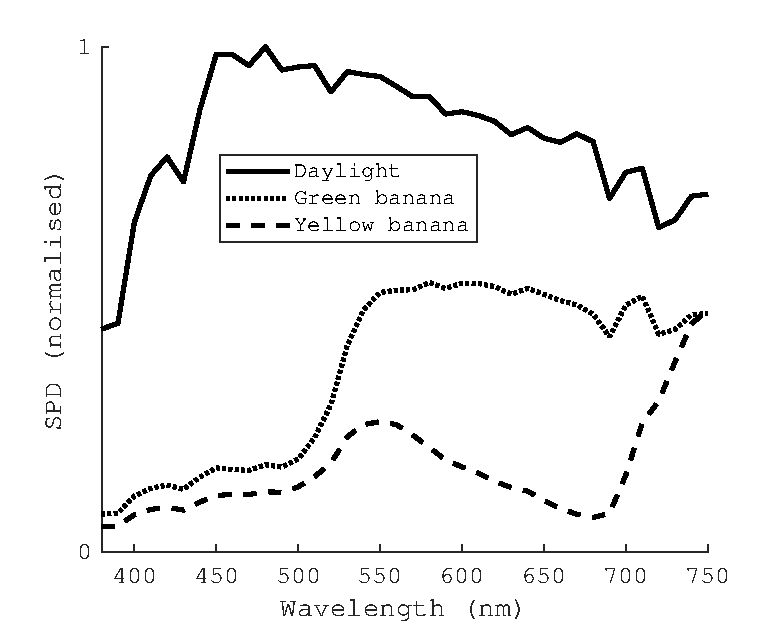
\includegraphics[max width=\textwidth]{figs/LitRev/daylightAndBananas.pdf}
\caption{The \gls{SPD} of a single measurement of daylight (sunlight plus scattered blue-sky light, from \citet{hernandez-andres_color_2001}) and the light reflected from 2 different surfaces - a green banana and a yellow banana (data from personal correspondence with David Slaughter after \citet{li_optical_1997}), computed by multiplying the \gls{SPD} by the measured \glspl{SRF} of the two surfaces. \Glspl{SPD} normalised such that the max of the daylight \gls{SPD} is 1.}
\label{fig:SPD}
\end{figure}

Our perception of colour generally correlates with the way in which objects preferentially reflect some wavelengths over others (described by the \acrfull{SRF}) which assists in the recognition of objects (that's a banana) and the discrimination of distinct objects, often in a manner that it ecologically beneficial (that's a \emph{ripe} banana).

\newpage

\subsection{Colorimetry}

\textit{The current recommended source for colorimetry is \gls{CIE} document `\gls{CIE} 015:2018'\citep{cie_cie_2018}\footnote{Though as \citet{fairchild_cie_2019} notes, this document is `expensive and somewhat difficult to find', and as such I have been using a draft of the now superseded `\gls{CIE} 15.3:2004'\citep{cie_cie_2004-2} as my personal guide. All equations listed in this chapter come from this source.}. Whilst this is the authoritative reference, my personal opinion is that an understanding of \gls{CIE} colorimetry is best gained from an understanding of its history, and for this I recommend Janos Schanda's book `Colorimetry: Understanding the \gls{CIE} System' \citep{schanda_colorimetry_2007}. Another valuable, and perhaps more easily accessed, reference source is \citet{stockman_color_2010}.}

\bigskip

I define `colorimetry' as the study of the quantitative specification of colour. As a subjective, internal and anthropocentric concept, in order to measure anything meaningful and comparable, we use a standard observer, or more precisely, one of a number of defined standard observers \cite{cie_bs_2011}.

The classic standard observer was defined by the \gls{CIE} in 1931, following experiments by Wright and Guild \cite{wright_re-determination_1929, guild_colorimetric_1931}. Despite several more recently published standard observers, the 1931 observer is still much used, and I shall use it in the following example of how a basic colorimetric computation is performed.

\glsreset{SPD}
\glsreset{SRF}
\glsreset{CMF}
\glsreset{SSF}

An illuminant is defined by its \gls{SPD}, a surface by its \gls{SRF}, and the sensitivity of a sensor (such as a photosensitive cell in the retina, or a pixel in a camera) by its \gls{CMF} (or in the case that biologically based measurements are used - the \gls{SSF}).

\begin{figure}[htbp]
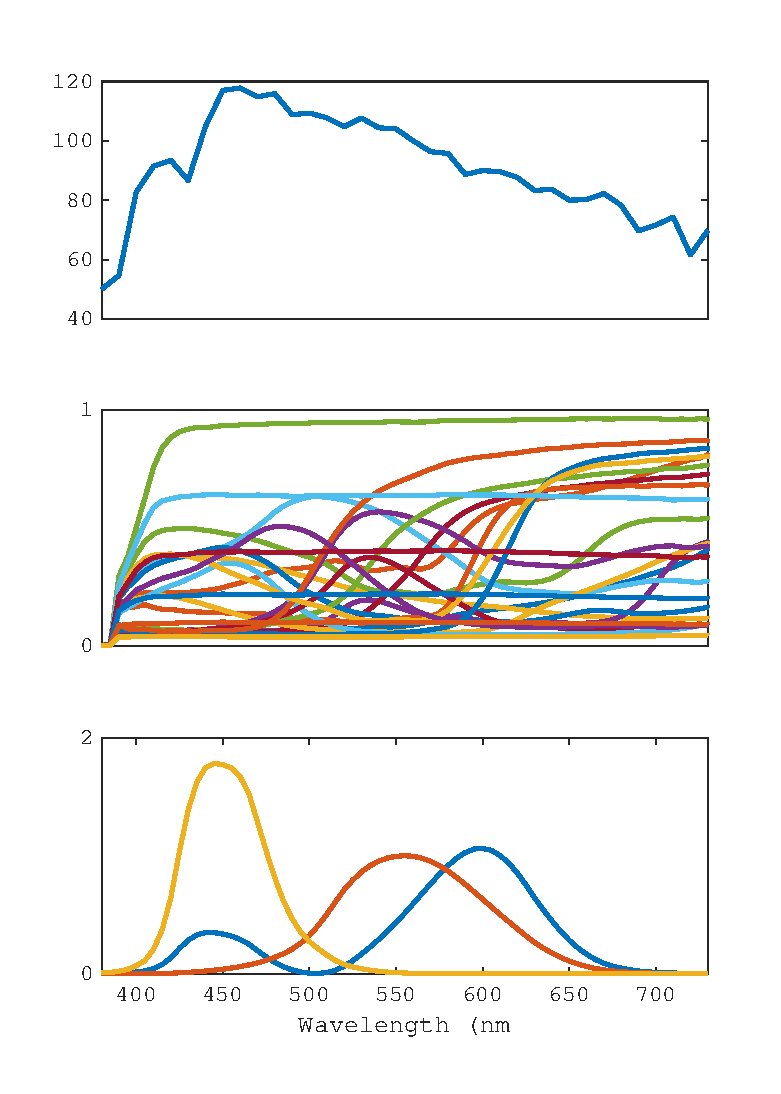
\includegraphics[max width=\textwidth]{figs/LitRev/SPDetc.pdf}
\caption{An \gls{SPD} (D65), a set of \glspl{SRF} (from a Macbeth Colour Checker) and three \glspl{CMF} (\gls{CIE} 1931 observer).}
\label{fig:specFun}
\end{figure}
% % How is D65 normalised here?

The light reaching the eye for a given reflecting surface under a given illuminant (termed the `colour signal') can be computed by multiplying the \gls{SPD} by the \gls{SRF} at each sampled interval.

\begin{equation}
\phi(\lambda)=R(\lambda) \cdot S(\lambda)
\end{equation}

where $R(\lambda)$ is the \gls{SRF}, $S(\lambda)$ is the \gls{SPD} and $\phi(\lambda)$ is the resulting colour signal. From this a set of values termed `tristimulus values' may be computed. Tristimulus values are computed by multiplying the colour signal by the \glspl{CMF} or \glspl{SSF}, and following the principle of univariance (that each cone type cannot alone distinguish between different wavelengths) the tristimulus values can, to some extent, be thought of as containing the entirety of the chromatic information about a surface (for a human standard observer, excluding high level colour appearance phenomena predicted by \Glspl{CAM}, and properties such as gloss).

%KC: make sure these equations are on the same page as the explanation 

\begin{subequations}
\begin{align}
X=k \sum_{\lambda} \phi(\lambda) \overline{x}(\lambda) \Delta \lambda \\ 
Y=k \sum_{\lambda} \phi(\lambda) \overline{y}(\lambda) \Delta \lambda \\ 
Z=k \sum_{\lambda} \phi(\lambda) \overline{z}(\lambda) \Delta \lambda
\end{align}
\label{eq:XYZ}
\end{subequations}

\nopagebreak %this doesn't work currently

where $\overline{x}(\lambda)$ (said `x bar'), $\overline{y}(\lambda)$ and $\overline{z}(\lambda)$ are the \glspl{CMF} of the 1931 observer (or are replaced by the \Glspl{CMF}/\Glspl{SSF} of the chosen observer), $\phi(\lambda)$ is as defined above, $k$ is a normalising factor, and $\Delta\lambda$ is 1nm. It is traditional to set $k$ such that $Y=100$, though in the case of relative colorimetry (most cases) this is often not done since the following equation renders it superfluous.

From the tristimulus values ($X,Y$ and $Z$) chromaticity co-ordinates ($x$ and $y$) can be computed. These can then be plotted on a 1931 chromaticity space diagram, shown as Figure \ref{fig:1931}.

\begin{subequations}
\begin{align}
x=\frac{X}{X+Y+Z} \\
y=\frac{Y}{X+Y+Z} 
\end{align}
\label{eq:1931chrom}
\end{subequations}

% Here's a \gls{MATLAB} example, using \gls{PTB} for data:

% \begin{lstlisting}[language=MATLAB]
% load spd_D65 % SPD: CIE D-series illuminant D65
% load sur_macbeth % SRF: macbeth colour checker
% load T_xyz1931 % CMF: CIE 1931

% colourSignals = sur_macbeth.*spd_D65;
% XYZ = T_xyz1931*colourSignals;
% xy = [XYZ(1,:)./sum(XYZ);XYZ(2,:)./sum(XYZ)];
% \end{lstlisting}

% Plotting: 

% \begin{lstlisting}[language=MATLAB]
% spectralLocus = [T_xyz1931(1,:)./sum(T_xyz1931);T_xyz1931(2,:)./sum(T_xyz1931)];
% sRGBSpectralLocus = XYZToSRGBPrimary(T_xyz1931);

% figure, hold on, 
% scatter(spectralLocus(1,1:70),spectralLocus(2,1:70),[],sRGBSpectralLocus(:,1:70)','filled')
% scatter(xy(1,:),xy(2,:),'k')
% axis equal, axis([0 1 0 1])
% xticks([0 1]), yticks([0 1])
% xlabel('x'), ylabel('y')
% \end{lstlisting}

\begin{figure}[htbp]
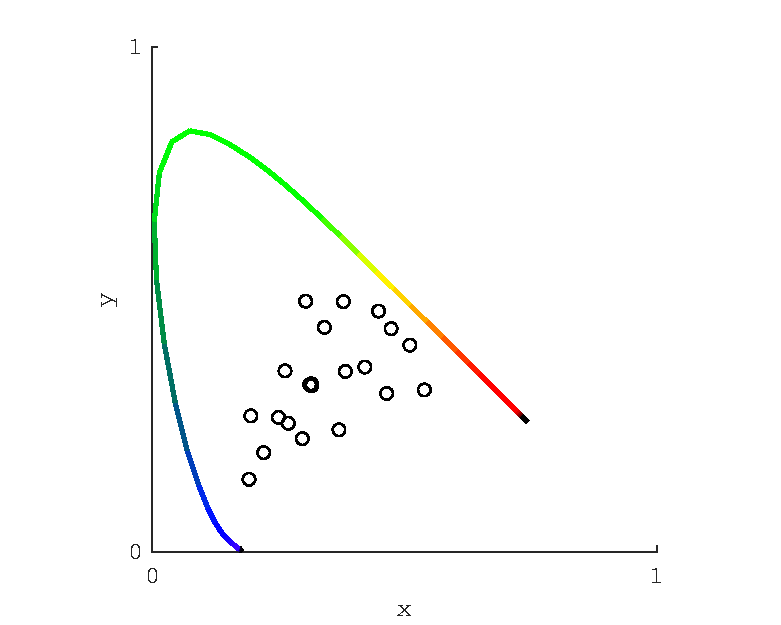
\includegraphics[max width=\textwidth]{figs/LitRev/ColorimetryDemo1.pdf}
\caption{The \gls{CIE} 1931 chromaticity space, showing the chromaticity of the Macbeth colour checker patches under D65. Note that for all of the plots in this section, the colours used for the spectral loci are only approximations.}
\label{fig:1931}
\end{figure}

\subsubsection{Specific Colour Spaces} \label{sec:speccolspac}

Over time various other colour spaces have been proposed and formally accepted by the \gls{CIE}, each aiming to improve upon a prior space in one or more ways. One of the most frequently sought characteristics for a colour space is perceptual uniformity, whereby a set distance in one part of the space is comparable in terms of apparent colour difference to that same distance in another part of the space.

One such chromaticity space which shall be used extensively in this thesis is the \gls{CIE} 1976 UCS (uniform chromaticity scale) space (colloquially \gls{CIE} u'v'), which is a relatively simple transformation of the 1931 chromaticity space. The conversion can be accomplished in a number of analogous fashions, one of which is shown below.

\begin{subequations}
\begin{align}
u' &= 4x / (-2x + 12y + 3) \\
v' &= 9y / (-2x + 12y + 3)
\end{align}
\end{subequations}

where $x$ and $y$ are the 1931 chromaticity co-ordinates as defined in Equation \ref{eq:1931chrom}. The data presented in Figure \ref{fig:1931} are re-plotted in this new space in Figure \ref{fig:UCS}.

\begin{figure}[htbp]
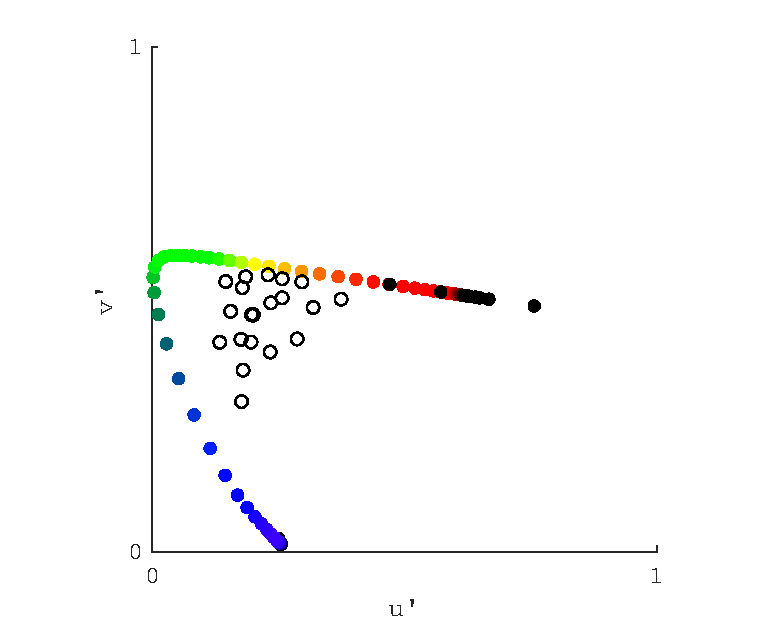
\includegraphics[max width=\textwidth]{figs/LitRev/ColorimetryDemo3.pdf}
\caption{\gls{CIE} 1976 UCS (uniform chromaticity scale) space, showing the chromaticity of the macbeth colour checker patches under D65 (as in Figure \ref{fig:1931}).}
\label{fig:UCS}
\end{figure}

A three-dimensional extension to the CIE 1976 UCS space is the \gls{CIE} 1976 L*u*v* colour space, often abbreviated to CIELUV, which aims to provide perceptual uniformity in a space that includes both chromaticity and lightness (relative to a white object under the same illumination). It is defined as follows:

\begin{subequations}
\begin{align}
L^{*} &= 116 f(Y/Y_{n})-16 \\
\textrm{where} f(Y/Y_{n}) &= (Y/Y_{n})^{1/3} &\textrm{ if } (Y/Y_{n}) > (24/116)^{3} \\
\textrm{or} f(Y/Y_{n}) &= (841/108)(Y/Y_{n})+16/116 &\textrm{ if } (Y/Y_{n}) \leq (24/116)^{3} \\
u^{*} &= 13L^{*}(u'-u'_{n}) \\ 
v^{*} &= 13L^{*}(v'-v'_{n})
\end{align}
\end{subequations}

where $Y_{n}$, $u'_{n}$ and $v'_{n}$ refer to the colour stimulus of a perfect reflector. The same data presented in Figures \ref{fig:1931} and \ref{fig:UCS} is presented in CIELUV in Figure \ref{fig:CIELUV} (though of course the three-dimensional quality of the data is somewhat lost in this presentation). 

\begin{figure}[hbtp]
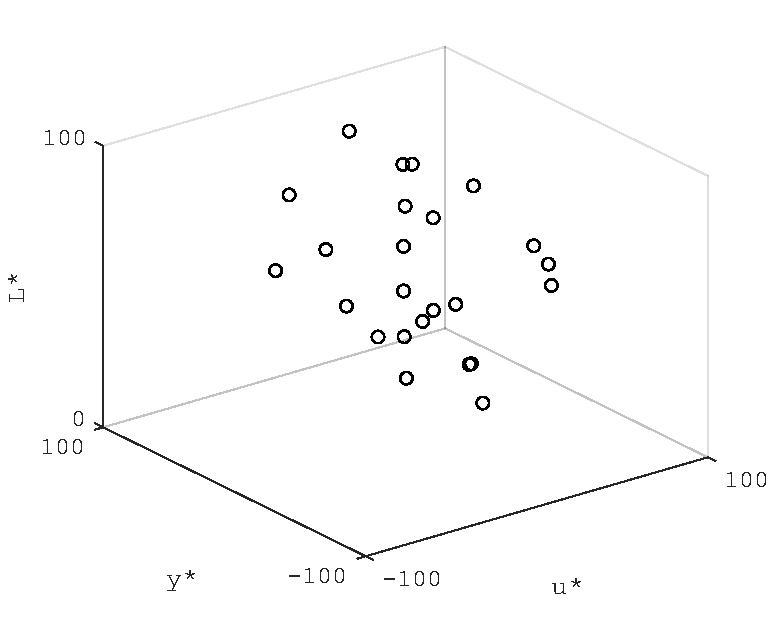
\includegraphics[max width=0.8\textwidth]{figs/LitRev/ColorimetryDemo4.pdf}
\caption{A representation of CIELUV, showing the values for the macbeth colour checker patches under D65 (as in Figure \ref{fig:1931} and \ref{fig:UCS}). Note that if viewed from above, the distribution of points would appear similar to as in Figure \ref{fig:UCS}. If all of the points were of uniform $L^{*}$, then the distribution would be identical, only with different scaling and offsetting.}
\label{fig:CIELUV}
\end{figure}

Introduced at the same time as CIELUV was a colourspace with a similar goal of perceptual uniformity: CIELAB. They are similar in many ways, and share $L^{*}$. CIELAB seems to be in slightly more common usage, but CIELUV is used in this thesis (particularly Chapter \ref{chap:Tablet}) due to the neat mathematical link to an associated chromaticity space (the CIE 1976 UCS space). 

The two spaces suit subtly different purposes, requested by two different user groups identified at the time of the creation of these spaces: ``lighting engineers interested in a space and formula that is a linear transformation of the CIE chromaticity diagram, and industrial colorists interested in a formula predicting perceived average color differences better than any existing one'' \citep{kuehni_color_2008}. CIELUV satisfied the first group, and CIELAB was designed to better suit the second, using a cube root function for the chromaticity values, mirroring $L^{*}$. CIELAB is defined as follows:

\begin{subequations}
\begin{align}
L^{*} &= 116 f(Y/Y_{n})-16 \\
\textrm{where} f(Y/Y_{n}) &= (Y/Y_{n})^{1/3} &\textrm{ if } (Y/Y_{n}) > (24/116)^{3} \\
\textrm{or} f(Y/Y_{n}) &= (841/108)(Y/Y_{n})+16/116 &\textrm{ if } (Y/Y_{n}) \leq (24/116)^{3} \\
a^{*} &= 500[f(X/X_{n}) - f(Y/Y_{n})] \\ 
b^{*} &= 200[f(Y/Y_{n}) - f(Z/Z_{n})] 
\end{align}
\end{subequations}

where $f(X/X_{n})$ and $f(Z/Z_{n})$ follow the same format as $f(Y/Y_{n})$.

The final colour space presented here is the \acrfull{MB} colour space. This space does not aspire to be perceptually uniform\footnote{This can be clearly noted by comparing Figure \ref{fig:lrMB} with previous figures. Where this set of chromaticities previously spanned the spaces fairly broadly, here all the chromaticities inhabit only a small portion of the chromaticity space.}. Instead, it aspires to provide a colour space which has a physiological underpinning. As such, the standard observer model consists of nominal \glspl{SSF} (rather than \glspl{CMF}), and the conversion from tristimulus values to chromaticity space attempts to mirror the way in which this actually occurs physiologically.

It was originally proposed by \citet{macleod_chromaticity_1979}, but was recently revised and endorsed by the \gls{CIE}, in documents `CIE 170-1:2006' \citep{cie_cie_2006} and `CIE 170-2:2015' \citep{cie_cie_2015}\footnote{I understand that the final publication in the series (`CIE 170-3:XXXX') is in preparation.}. The revisions included the definition of a new observer (formally the `TC 1-36 Modified Colorimetric Observer', colloquially refered to as the \gls{CIE} 2006 observer), based on the work of \citet{stockman_spectral_1999} and \citet{stockman_spectral_2000} (and referred to below as $\overline{lms}$), and the introduction of a set of new normalising terms, such that it is now calculated as follows.

\begin{subequations}
\begin{align}
L_{\text{MB}}&=k_{l} \sum_{\lambda} \phi(\lambda) \overline{l}(\lambda) \Delta \lambda \\ 
M_{\text{MB}}&=k_{m} \sum_{\lambda} \phi(\lambda) \overline{m}(\lambda) \Delta \lambda \\ 
S_{\text{MB}}&=k_{s} \sum_{\lambda} \phi(\lambda) \overline{s}(\lambda) \Delta \lambda
\end{align}
\label{eq:MBTristim}
\end{subequations}

where $k_{l}$ = 0.68990272, $k_{m}$ = 0.34832189, $k_{s}$ = 0.03715971. This set differs minimally but purposefully from Equation \ref{eq:XYZ}; in the choice of observer ($\overline{lms}$), and in the use of different scaling factors for each tristimulus value. The different scaling values dictate the relative contributions of $L_{\text{MB}}$ and $M_{\text{MB}}$ to luminance, and constrict $s_{\text{MB}}$ to a maximum value of 1 in the following equation (Equation \ref{eq:MB}). \gls{MB} chromaticity values are then calculated as follows:

\begin{subequations}
\begin{align}
l_{\text{MB}}&= \frac{L_{\text{MB}}}{L_{\text{MB}}+M_{\text{MB}}} \\ 
s_{\text{MB}}&= \frac{S_{\text{MB}}}{L_{\text{MB}}+M_{\text{MB}}} 
\end{align}
\label{eq:MB}
\end{subequations}

Whereas the relationship between the axes of previous colour spaces was important, here the axes are nominally independent (representing different post-receptoral mechanisms) and so the scaling between the axes is arbitrary. As such, in vision science the axes of this diagram are often re-scaled to suit the task at hand (see for example \citet{christiansen_chromatic_2017,bosten_what_2015,danilova_superior_2016}). The same data as presented previously is presented again in Figure \ref{fig:lrMB} in a \gls{MB} chromaticity space.

\begin{figure}[htbp]
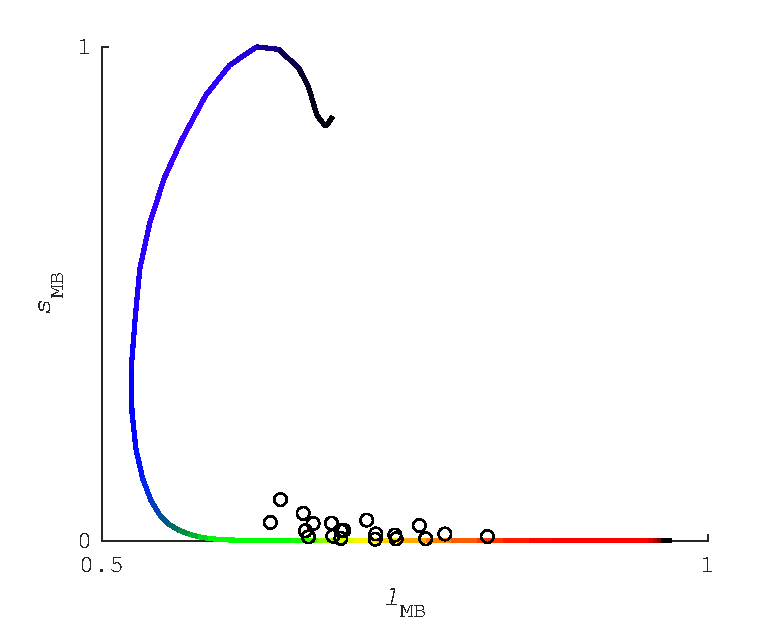
\includegraphics[max width=\textwidth]{figs/LitRev/ColorimetryDemo5.pdf}
\caption{A \gls{MB} chromaticity space diagram (as per \gls{CIE} 170-2:2015 \citep{cie_cie_2015}) showing the values for the macbeth colour checker patches under D65, as in previous figures.}
\label{fig:lrMB}
\end{figure}

\subsubsection{Correlated Colour Temperature}

The \acrfull{CCT} of an illuminant is defined by CIE 15.3:2004 \citep{cie_cie_2004-2} as follows:

\begin{itquote}{}
The temperature of a Planckian radiator having the chromaticity nearest the chromaticity associated with the given spectral distribution on a diagram where the (CIE 1931 standard observer based) u', 2/3v' coordinates of the Planckian locus and the test stimulus are depicted.
\end{itquote}

Whilst by this definition a light source of any chromaticity could be assigned a \gls{CCT}, as the distance between the Planckian locus and the test stimulus increases, the \gls{CCT} becomes a less meaningful descriptor. CIE 15.3:2004 \citep{cie_cie_2004-2} defines chromaticity limits on the maximum distance between the Planckian locus and the test stimulus, beyond which \gls{CCT} should not be used, which are described in Equation \ref{eq:CCTlim}.

\begin{equation}
\Delta C=\left[\left(u_{t}^{\prime}-u_{P}^{\prime}\right)^{2}+\frac{4}{9} \cdot\left(v_{t}^{\prime}-v_{P}^{\prime}\right)^{2}\right]^{1 / 2}=5 \cdot 10^{-2}
\label{eq:CCTlim}
\end{equation}

where $u^{\prime}_{t}, v^{\prime}_{t}$ refer to the test source and $u^{\prime}_{P}, v^{\prime}_{P}$ to the Planckian radiator.

Figure \ref{fig:BBR} shows Planckian locus (the curve formed by a set of black body radiators of different temperatures) in \gls{CIE} 1931 chromaticity space. It is worth noting that most real light sources (natural and artificial) fall upon the relatively straight section of the left-hand part of this line.

\gls{CCT} is often used as the independent variable in experiments, with the implicit assumption that this can be considered a complete descriptor of a light source. This assumption only holds to the extent that the spectral form is similar between conditions (for example if only a single light source is used and well defined filtration is applied, which shifts the chromaticity of the light source along the Planckian locus), and that the only difference between conditions is a shift along the Planckian locus. 

A shift in chromaticity perpendicular to the Planckian locus would result in no change to the \gls{CCT}. To counter this issue, an additional parameter ($D_{\text {uv }}$) is defined \citep{ohno_practical_2014} as per Equation \ref{eq:Duv}, which provides a value for the distance from the Planckian locus.

\begin{equation}
D_{\mathrm{uv}}=\left[\left(u^{\prime}-u_{0}^{\prime}\right)^{2}+\left(\frac{2}{3} v^{\prime}-\frac{2}{3} v_{0}^{\prime}\right)^{2}\right]^{\frac{1}{2}} \cdot \operatorname{sgn}\left(v^{\prime}-v_{0}^{\prime}\right)
\label{eq:Duv}
\end{equation}

where $\operatorname{sgn}(z)=1$ for $z\geq0$ and $\operatorname{sgn}(z)=-1$ for $z<0$.

\citet{ohno_practical_2014} notes that the combination of \gls{CCT} and $D_{\text {uv }}$ is suffice to describe the chromaticity of most light sources, and does so in a fashion which is slightly more intuitive than values of chromaticity.

\begin{figure}[htbp]
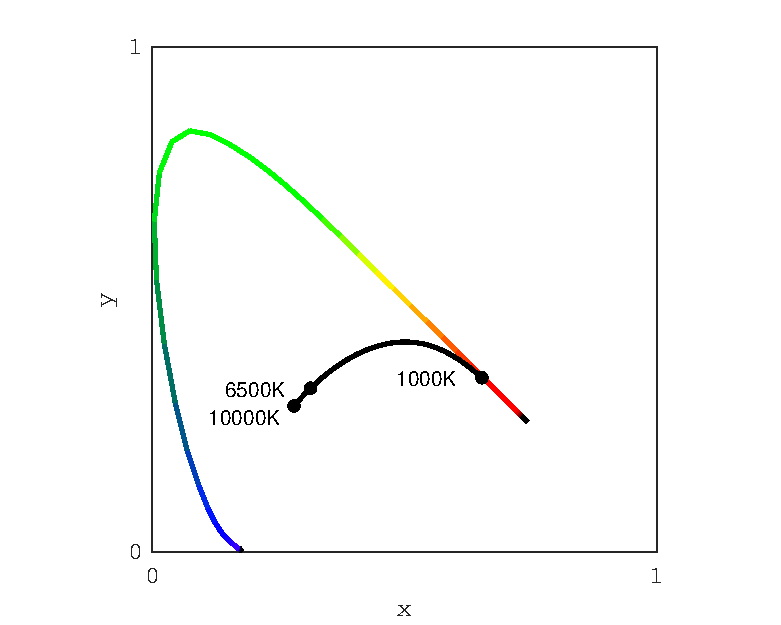
\includegraphics[max width=\textwidth]{figs/LitRev/BBR.pdf}
\caption{The Planckian locus on a \gls{CIE} 1931 chromaticity chart, highlighting \glspl{CCT} of 1000K, 6500K and 10000K.}
\label{fig:BBR}
\end{figure}

\clearpage
\subsection{Colour rendering}

Colour rendering indices provide an indication of the colour appearance of objects under a test illumination. Colour fidelity indices (properly a subset of colour rendering indices, however the most commonly used colour rendering index is in fact a colour fidelity index) are designed to describe how well a light source will produce a faithful appearance in terms of corresponding colorimetry to an appearance under \gls{CIE} D-series illuminant (daylight proxy) or a black body radiator. %Target values are generally provided in museum lighting guidelines \citep{ies_ies_1996,druzik_guidelines_2012,cibse_lighting_2015,thomson_museum_1986}. The recommended value for the ubiquitously used \gls{CIE} R\textsubscript{a} (As defined in \gls{CIE} 13.3:1995 \citep{cie_cie_1995}), often informally referred to as `CRI', varies from publication to publication, but is generally \gls{CIE} R\textsubscript{a}$>$80, but with no experimental work referenced to support this figure. 
Research in colour rendering is at a point of change and development, with the recognition that a single figure might never be enough to describe the complex, multidimensional, subjective and context dependent qualia of colour rendering\citep{rea_color_2008}. Thus new indices, and modifications and addenda to long-established indices are being proposed \citep{smet_memory_2012,davis_color_2010,rea_practical_2010,ies_ies_2015,teunissen_characterising_2016}.

If we were to take a bunch of balloons (or any objects, but balloons provide a simple and vivid image) of varied and multiple colours, from an area lit with daylight to an area lit with artificial light, and the colour appearance changes, for example the colours become more dull, we would generally be disappointed. In this case, we could say that we were dissatisfied by the colour rendering qualities of the artificial light source. If the colours remained the same we probably would think little of it, but if we were pressed for a comment, we might say that the colour appearance was satisfactory. 

If the balloons stayed the same colour as they had been under daylight, we would be witnessing a high level of colour fidelity (fidelity meaning faithfulness or truthfulness). If fidelity aligns well with the priorities of the user, then high levels of fidelity are desirable. If the appearance of the balloons had changed in some other way than becoming more dull - for example the colours became more vivid or the hue of certain balloons changed drastically, we might not neccessarily be disappointed, but this would still represent a situation where we were witnessing poor fidelity.

Generally when discussing colour fidelity, we are actually discussing fidelity to appearance under daylight or sometimes a Planckian radiator, aka a black body radiator. This is a fine comparison, but one which should be consciously considered; fidelity is not a measure of a light source per se, it is a comparison of that light source to a reference illuminant.

Fidelity has long been considered semi-analogous for colour rendering as a whole, but it is really only one element of colour rendering\footnote{Here I should point out that the \gls{CIE} definition of colour rendering, from the publication \gls{CIE} S 017/E:2011 ILV: International Lighting Vocabulary \citep{cie_cie_2011} reads: ``Effect of an illuminant on the colour appearance of objects by conscious or subconscious comparison with their colour appearance under a reference illuminant.'' You might notice the similarities to the definition I have ascribed to colour fidelity, and specifically not colour rendering. This is an unfortunate clash of nomenclature which I see as inappropriate usage on the part of \gls{CIE}, and at some point I hope this official definition will be updated to match the modern vernacular.}. When considering how `good' a light source is at facilitating colour with the objects which it illuminates, we might consider different measures alongside or in place of fidelity.

\begin{itemize}
\item \emph{Colour Fidelity (to recap)} - A measure of comparison between how colours appear under daylight (or other reference) and how they appear under another light source. %Do the balloons appear the same colour indoors and out? Are individual colours important or is an average suitably representative?
\item \emph{Chromatic Discrimination} - The ability of a light source to illuminate objects such that subtle differences in colour are made most visible. %Can you tell the difference between all the balloons? How big are the differences? Are threshold differences more or less important than the perceived magnitude of suprathreshold differences?
\item \emph{Observer Preference} - Subjective preferences for the colour of objects, potentially related to an increase in saturation, or an observer's memory of colours, or specific colour effects (e.g. increased saturation of skin tones). %Do the balloons look `nicer'/more vivid/more like the last time you saw them?
\end{itemize}

These areas overlap, and often exhibit correlation. For example, if a light source has properties which allow for high fidelity rendering, quite often that light source might also allow for good colour discrimination and also facilitate colours which might appear natural and/or pleasing. These are not reliable correlations however; it is quite possible to have a light source with very dissimilar properties to daylight that could score highly on discrimination and/or preference, or vice versa.

The index in widest use currently for quantifying colour rendering is \gls{CIE} R\textsubscript{a} (The General Colour Rendering Index). At the beginning of this doctoral project, this metric was used almost exclusively to generate the figure listed as `CRI' on the packaging for bulbs available commercially. %In the intervening time, IES RP-30-15 \citep{ies_ies_2015}, and more recently IES RP-30-18 \citep{ies_ies_2018}, have been published and have found considerable uptake from manufacturers.

\gls{CIE} R\textsubscript{a} is a colour fidelity metric, produced by computing the colour differences of 8 specified test colour samples (TCSs), between the situation where illumination is provided by the test source and that where it is provided by a reference illuminant with the same \gls{CCT} as the test source, and taking the arithmetic mean of these colour differences. The index is scaled such that the highest score is 100, for light sources which reproduce the TCSs under the reference illuminant exactly, with any light source which induces a colour shift receiving a value less than 100, descending below 0 if the magnitude of the shifts are great enough.

The most recent version of the standard specifying this metric is `\gls{CIE} 13.3-1995 Method of Measuring and Specifying Colour Rendering Properties of Light Sources' \citep{cie_cie_1995}. This document briefly overviews the history of, and necessity for, a colour rendering index and highlights areas of the procedure which vary compared to previous recommendations, and clearly details the recommended procedure. The process is summarised in the flow chart of Figure \ref{fig:criflow}. For a worked example see \citet[p.388]{hunt_measuring_2011}.

In response to a lack of confidence that \gls{CIE} R\textsubscript{a} delivered meaningful values for LED illumination, a considerable amount of research and discussion has revolved around the subject of a colour rendering index to supersede \gls{CIE} R\textsubscript{a}. This is commonly complicated by the incorrect assumption that the values obtained from a fidelity index in some way correlate with preference. A more valid criticism of \gls{CIE} R\textsubscript{a} is that it comprises deprecated methods and data sets for computing intermediary stages within the process of calculation, and thus this theoretically limits the `correctness' of any values produced by it.

Following many years where multiple \gls{CIE} technical committees aimed to deliver updated colour rendering indices, but subsequently didn't make any firm recommendations, an IES group was formed with the aim of examining the issue. The output of this IES group was the production of IES TM-30-15\cite{ies_ies_2015}, which follows the same philosophy as \gls{CIE} R\textsubscript{a} but with more modern colour science. It is still a contentious issue whether this updated index genuinely offers advantages over \gls{CIE} R\textsubscript{a}. 
% it also includes a bunch of other things...
% and IES TM-30-18?

Alternative propositions which offer fundamentally different approaches to the evaluation of colour rendering have been offered in recent years, including: 
\begin{itemize}
\item indices based on production of memory colours \citep{smet_memory_2012}.
\item indices which consider the size of the gamut of a TCS set \citep{rea_color_2008,teunissen_characterising_2016}.
\item indices which are fundamentally fidelity indices but which penalise or reward specific traits known to be disliked/preferred \citep{ohno_rationale_2010}.
\end{itemize}

\begin{figure}[htbp]
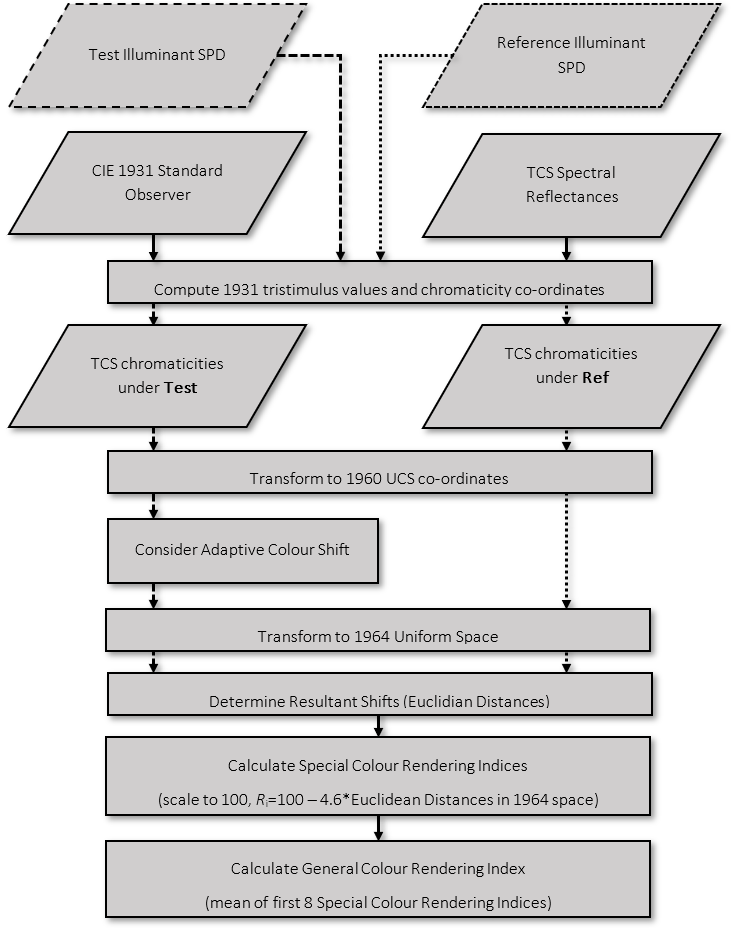
\includegraphics[max width=\textwidth]{figs/LitRev/criflow.png}
\caption{The stages of calculation for the computation of the \gls{CIE} General Colour Rendering Index. Notes: Reference illuminant: the same or nearly the same \gls{CCT}. Below 5000K reference spectrum will be that of a black body radiator, and from 5000K `one of a series of spectral power distributions of phases of daylight'.}
\label{fig:criflow}
\end{figure}

\clearpage

\subsection{Chromatic Adaptation and Colour Constancy}

\textit{Shortly after the start of my PhD program I attended a symposium for PhD students in the field of lighting research (LumeNet). At this symposium Prof. Michael Pointer delivered a welcome talk, and one particular part of it stuck with me.}

\textit{He described how at the start of his PhD studies \citep{pointer_colour_1972}, he had made copies of every paper which had been written on his subject (Chromatic Adaptation) which were available from the library, and written to any authors whose work he had been unable to access, requesting copies. At the end of his first year he had a binder which contained, as far as he was aware, everything ever written on the subject. He finished his story rather abruptly, along the lines of ``since then, so many people have written on the subject that it would take much longer than you have within a PhD program to read it all. I don't know what you all will do''. Not an encouraging thought!}

\textit{With this in mind, I shall attempt only to cover the basics and a few select papers of particular relevance in the following section, and shall take this opportunity to note my debt to a number of comprehensive overview papers, book chapters and theses on this subject: \citet{foster_color_2011,maloney_computational_1984,barnard_practical_1999,smithson_sensory_2005,hurlbert_computational_1998,brainard_color_2014,fairchild_color_2013}.}

\subsubsection{The problem}

At the start of this section I stated that ``Our perception of colour generally correlates with the way in which objects preferentially reflect some wavelengths over others''. It transpires that this ability is non-trivial, because our visual systems do not have access to the \glspl{SRF} of the objects which are seen, only the levels to which retinal cells are excited, which depends on the interaction of illuminant, surface and sensor. 

Figure \ref{fig:problem} demonstrates the problem, by reproducing Figure \ref{fig:1931} with a minor adjustment; where the previous figure had the chromaticities of the set of surfaces under only a single illuminant, a large number of illuminants are used here. It can be seen that it is not uncommon for one surface to have a chromaticity under one illuminant that another surface has under a different illuminant. Thus, the relationship between surface and chromaticity appears to break down.

\begin{figure}[htbp]
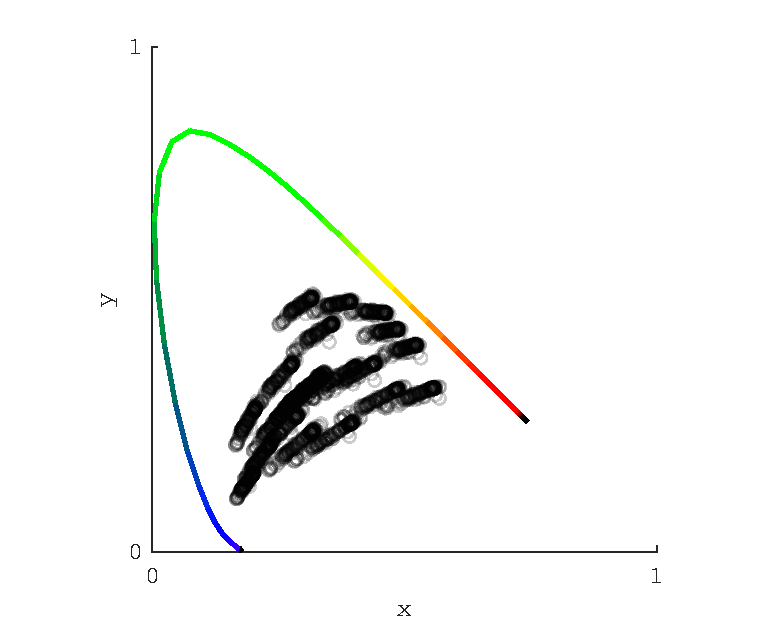
\includegraphics[max width=\textwidth]{figs/LitRev/ColorimetryDemo6.pdf}
\caption{A reproduction of Figure \ref{fig:1931}, but this time with the chromaticity co-ordinates for the 24 macbeth colour checker patches under a range of daylights, drawn from the Granada dataset \citep{hernandez-andres_color_2001} (further described in Section \ref{sec:coldata}).}
\label{fig:problem}
\end{figure}

In order to provide a representation of colour where the perceived colour remains constant across changes in illuminant (thus the term \emph{colour constancy}), the human visual system must find a way to solve this problem.

\subsubsection{Adaptation}

`Adaptation' is the general mechanism by which a finite range of sensitivity can be shifted within absolute sensitivity bounds. The benefit of having an adaptive system, as opposed to a fixed system, is that the sensitivity of the system to small changes is maximised, whilst maintaining a broad overall sensitivity, at the expense of being able to sense over the entire range at a single time-point. A visual demonstration of this is shown in Figure \ref{fig:Valeton} where it can be seen that that at a single level of adaptation (a single line) the range of intensity over which responses are generated is relatively small, but is extended through adaptation.

\begin{figure}[htbp]
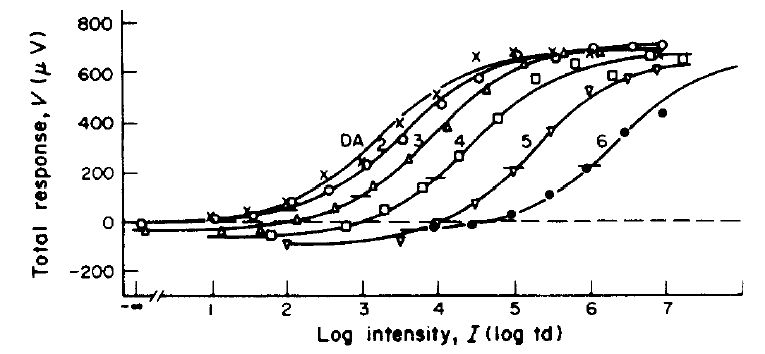
\includegraphics[max width=\textwidth]{figs/LitRev/Valeton.png}
\caption{Cone flash response at different levels of adaptation in macaques, reproduced from \citet{valeton_light_1983}. On the left `DA' stands for dark-adapted, with the rising numbers for the other lines relating to rising adapting levels.}
\label{fig:Valeton}
\end{figure}

In an environment such as the terrestrial environment, there is a great range in the level of illumination, but this range is rarely existent contiguously; levels of illumination tend to be similar across a scene, and only change rather slowly over time. The notable exception, and thus where we notice the expense of having an adaptive visual system, comes when we enter or exit an environment where illumination is almost entirely excluded, such as a dark cave or below-decks of a boat. 

Where the process of adaptation responds to overall illumination levels, it is referred to as light adaptation and dark adaptation. Where the process of adaptation responds to the wavelength composition of light reaching the eye it is referred to as chromatic adaptation.

In a natural environment, a change in the wavelength composition of radiation reaching the eye from a specific object might be caused by changing weather or time of day, or by the physical movement of the object from one space to another (where different lighting exists in the two different spaces). Figure \ref{fig:SPDnorm} shows a set of measured daylight \glspl{SPD}, normalised by luminance, showing that the wavelength composition varies quite considerably, though in a relatively systematic fashion.

\begin{figure}[htbp]
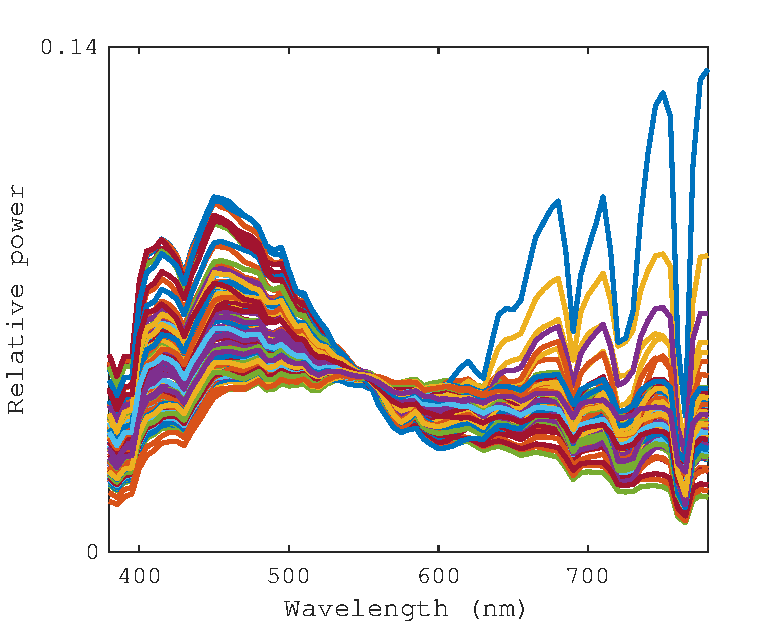
\includegraphics[max width=\textwidth]{figs/LitRev/ColorimetryDemo7.pdf}
\caption{The \glspl{SPD} of a subset of the daylight measurements of \citet{hernandez-andres_color_2001} (further described in Section \ref{sec:coldata}), normalised by luminance.}
\label{fig:SPDnorm}
\end{figure}

\subsubsection{Mechanistic vs. Inferential}

In the literature there seems to be a long-running grapple between colour constancy and chromatic adaptation, with blurred boundaries and mixed definitions occurring frequently. \citet{brill_chromatic_1986} drive a wedge between the two concepts, but refute the traditional division that chromatic adaptation is the process and colour constancy is the ability, asserting that the two should be considered as separate processes, operating on different timescales and in different fashions.

\citet{hurlbert_computational_1998} divides computational models of colour constancy into two classes: \emph{sensory} and \emph{perceptual}, which broadly follow the low-level / high-level divide. `Sensory' models `could be achieved early in visual processing by adaptive scaling of the initial receptor responses'. `Perceptual' models `would necessarily occur at later stages of visual processing'.

Hurlbert [personal communication] notes that understanding the differing perspectives of researchers from different fields allows one to understand how the mixed use of these terms in the literature may have arisen: 

\begin{itquote}{}
The mixed use of the terms chromatic adaptation and colour constancy is largely explained by different usages in different fields. In \emph{colour science}, chromatic adaptation is often considered synonymous with colour constancy, as it is considered to be the only mechanism contributing to stabilising colour appearance under changes in illumination. In \emph{vision science}, colour constancy is generally defined as a perceptual phenomenon, and distinction is made between different contributory mechanisms at different levels (which \citet{hurlbert_computational_1998} attempts to define and onto which different proposed computational solutions are mapped).
\end{itquote}

Within vision science, the most common use of the term `chromatic adaptation' now seems to be to refer to low level adaptation, with \citet{brainard_color_2014} using the term `mechanistic' to refer to this type of transformation.

\begin{itquote}
Adaptation of this sort supports constancy to the extent that its overall effect is to stabilize the post-receptoral representation of the light reflected from objects across changes of illumination (as well as other contextual changes).
\end{itquote}

The term `colour constancy', by contrast, is used to refer to higher level inference-based processes, which occur at faster timescales than are possible by adaptation alone \citep{rinner_time_2000}. It seems likely that multiple processes work in tandem at multiple levels and timescales to achieve colour constancy \citep{hurlbert_colour_2007}.



\subsubsection{Von Kries Adaptation}

The conceptually simplest model of chromatic adaptation, and the forefather of many other models, is that referred to as Von Kries adaptation.

Johannes von Kries was one of the first to deeply consider chromatic adaptation, and appears to have understood it as a problem of sensory adaptation. In his formative series of papers, available in translation \citep{von_kries_beitrag_1970}, he laid out how the study of chromatic adaptation could be divided into two broad and complementary aims. 

The first referred to the systematic representation of the transforms in sensation caused by specific adaptations, such that \textit{``for any light mixture stimulating the readapted part [of the retina], another light mixture is specified that stimulates the same sensation in a normally adapted part \dots The purpose of this study would be solved completely if a general rule could be obtained for the effects of all possible adaptions.''} The search for `corresponding colours' (pairs of colours which match under asymmetric adaptation states), and for suitable systems to predict the appearance of colours in all situations, fall within this category of exploration. Out of this aim grew the study of \glspl{CAT}, where the search for an algorithm which would mathematically predict the locations in colour space of corresponding colours has been the fundamental goal \citep{cie_tc_1-52_cie_2004}.

Von Kries suggested that the second categorical aim of chromatic adaptation research ought to be to discover `how the adaptation is produced by exposure to any particular color, continued over an extended period of time.' 

Von Kries' distinction carves a divide between the study of the mechanisms of chromatic adaptation, and the effects of chromatic adaptation. It would be unreasonable to think of these areas of study as unrelated, but it seems reasonable to recognise their separability. 

%In the same set series of papers, von Kries laid out his understanding of chromatic adaptation, in terms of both how corresponding colours might be calculated, and how one might consider the underlying mechanisms which allow for colour constancy to operate. Here I shall abridge some of his writings to present the most salient insights, and attempt to explain what is meant by a `von Kries transform' in modern parlance.

Von Kries noted that `light mixtures that appear matched to the white-adapted eye always remain matched to the eye when it is adapted in any other manner.' This is known to be only partly true; if referring to photopic vision solely (where rods are bleached and cones provide the basis for vision). The implication of this statement is that the spectral sensitivities of the cone cells do not change as a result of chromatic adaptation. If they were to change in some way, then distinct mixtures of light which match in one adaptive state might fail to match under a different state. Von Kries referred to this idea as the `persistence rule.'

The second rule which von Kries presents is referred to as the `theorem of proportionality'. This theorem claims that when two pairs of corresponding colours (colours A and B under illuminant 1, and colours C and D under illuminant 2) are additively combined (A with B, and C with D), the resulting colours will also be corresponding colours. It follows from the von Kries' theorem of proportionality that increasing or decreasing the luminance of corresponding stimuli shouldn't void their equality, though of course this statement relies even more heavily on the caveat that this should only be assumed for photopic vision.

Von Kries goes on to suggest that it also follows that, if considered in combination with Grassmann's law \citep{grassmann_zur_1853}, the conversion of any arbitrary light by exposure to conditions causing a specific chromatic adaptation can be known if the nature of three other conversions are known. This relies on it being possible to consider any light as a linear combination of three others, and for the mechanism of chromatic adaptation to depend solely on the fatiguing of three independent systems.

Von Kries' assertions may be mathematically described as:

\begin{subequations}
\begin{align}
L_{a}&=K_{L}L \\
M_{a}&=K_{M}M \\
S_{a}&=K_{S}S
\end{align}
\end{subequations}

where $L$, $M$ and $S$ represent the cone group responses; $K_{L}$, $K_{M}$ and $K_{S}$ represent distinct scalars and $L_{a}$, $M_{a}$ and $S_{a}$ represent the post adaptation cone group responses\footnote{This specific notation is taken from \citet[p. 183]{fairchild_color_2013}.}. In terms of what might set these scalars, or gain values, von Kries suggested that: 

\begin{itquote}{von_kries_beitrag_1970}
the organ of vision becomes less effective for that kind or for that part of its performance which is demanded from it for an extended period of time, whereas it becomes more effective for the activity which is, in a sense, opposed to that. This can be conceived in the sense that the individual components present in the organ of vision are completely independent of one another and each is fatigued or adapted exclusively according to its own function.
\end{itquote}

Many interpretations have been made of this statement, and a corresponding number of nominations for methods by which to calculate values of $K$ have been proposed. The most frequently considered methods are those referred to as \acrfull{GW} (where the reciprocal of the mean response across a scene is used) and \acrfull{BiW} (where the reciprocal of the brightest point in the scene is used). \citet{finlayson_shades_2004} showed that these two variants can be considered as part of a single framework (Minkowski norm), and that other members of this family of algorithms provide benefits over \gls{GW} and \gls{BiW}.

Von Kries' thoughts have inspired many decades of research into \glspl{CAT}, which are a vital part of modern colour appearance models and other colour science computations, such as colour rendering index calculations. This relatively simple concept has remained relevant, as noted by \citet[p. 182]{fairchild_color_2013} who reproduces this quote:

\begin{citequote}{von_kries_beitrag_1970}
If some day it becomes possible to distinguish in an objective way the
various effects of light by direct observation of the retina, people will perhaps
recall with pitying smiles the efforts of previous decades which
undertook to seek an understanding of the same phenomena by such
lengthy detours.
\end{citequote}

followed by the comment:

\begin{citequote}{fairchild_color_2013}
Over eleven decades later, there is no one looking back at von Kries' work
with a ``pitying smile''. Rather, many are looking back at his work with
astonishment at how well it has withstood the test of time.
\end{citequote}

\subsubsection{Retinex}

Considered in the context on von Kries' work, the Retinex model of Land et al. \citep{land_retinex_1964,land_lightness_1971,land_recent_1983,land_recent_1986,mccann_quantitative_1976} might be described as `Von Kries adaptation with spatial considerations' but I imagine such a statement would have rather riled the often bombastic sounding Land. It appears to have been Land's understanding that the Retinex model was not a model of chromatic adaptation, but rather a model to usurp and do away with the very concept of chromatic adaptation (Land's papers on the subject \citep{land_retinex_1964,land_lightness_1971,land_recent_1983,land_recent_1986} do not once use the term `chromatic adaptation', nor is the work of von Kries ever explicitly referred to). 

Land was fond of picking apart Newton's statements regarding colour; particularly that the perception of colour was the result of an objects' `excess and predominance in the [spectra of the] reflected light' \citep{newton_opticks_1704}. Land asserted that rather than work from the premise that the visual system was correcting an absolute record of the world, by normalising it to account for the ambient light source, one should instead consider visual input only as a relative record, where each element within a scene only takes on properties by comparison with the other elements of the scene. 

He suggested for consideration the idea of the human visual system recording three separate lightness images, each representing the recording from a different band of receptors, where each element within each image is scaled against the brightest element in each specific image. Retinex theory also provides an interesting algorithm for discounting not only coloured illumination but illumination which varies across the visual field.

However, \citet{barnard_practical_1999} points out that the various versions of the Retinex algorithm simplify to versions of the Von Kries adaptation, and \citet{brainard_analysis_1986} found that `the algorithm is too sensitive to changes in the color of nearby objects to serve as an adequate model of human color constancy'. In addition, it has been found to be computationally difficult to implement, with no clear way in which it could be biologically implemented (though see \citet{hurlbert_formal_1986}).

The work of Land et al. has spurred a great deal of progress in the world of digital imaging, where the term `computational colour constancy' is used. The number of distinct algorithms increases at a rate which seems to always accelerate, and I shall not review them all here, though I shall point to valuable overview papers:  \citet{hordley_reevaluation_2006, gijsenij_computational_2011, hurlbert_computational_1998}.

\subsubsection{Linear models}

If we extend the common interpretation of colour constancy (that colours should remain constant), to a stricter case where we actively try to recover the \glspl{SRF} of surfaces, simple Von Kries-type transformations no longer suffice. \citet{maloney_physics-based_2001} and \citet{yang_illuminant_2001} discuss what they term the `RGB heuristic'. Simply put - this is the commonly held assumption that a set of cone catches under one illuminant will be related to a second set of cone catches under another by a transformation which can be fully described by the chromaticities of the illuminants. As \citet{maloney_physics-based_2001} says `there is no \emph{mathematical} reason to expect [this] to hold, even approximately'. This can be considered from the perspective of colour rendering; it is known that objects which are metamers under one illuminant might not be under another. This renders simple models of colour constancy ineffective. \citet{foster_frequency_2006} quantified the frequency of metamerism in real scenes and found it to be `sufficiently large to affect visual inferences about material identity'.

For this stricter definition of colour constancy Maloney et al. \citep{maloney_computational_1984, maloney_color_1986} propose a method which makes use of discrete linear models, whereby the set of real \glspl{SRF} and real \glspl{SPD} are approximated by a small number of fixed basis functions. 

\citet{maloney_color_1986} find that `with three classes of photoreceptors, we can exactly recover surface reflectances drawn from a fixed model of surface reflectance with at most two degrees of freedom'. \citet{maloney_computational_1984} showed that this generalised such that with $n$ classes of photoreceptors, \glspl{SRF} could be reconstructed for surfaces drawn from models with $n-1$ degrees of freedom, so long as there were not more than $n$ degrees of freedom in the illumination model, and so long as the minimum complexity condition was met (there were enough surfaces visible).

Despite its mathematical elegance, quantitative analysis of this algorithm showed that its performance was poor \cite{brainard_bayesian_1994, finlayson_color_1995}, which is not surprising considering that natural surface \glspl{SRF} generally require more than two basis functions for accurate reconstruction.

\bigskip

There are many further ideas, theories, and concepts relating to colour constancy and chromatic adaptation which are beyond the scope of this chapter, but that the reader may find of interest: gamut mapping algorithms \citep{forsyth_colour_1990,forsyth_novel_1990,forsyth_colour_1989,finlayson_color_1996}, bayesian colour constancy \citep{finlayson_color_2001, brainard_bayesian_2006,gazzaniga_bayesian_2009, brainard_bayesian_1994,gehler_bayesian_2008} and specular-reflectance-based algorithms \citep{mollon_monge_2006, morimoto_discrimination_2018,hurlbert_computational_1998}.

%% Removed stuff ---------------------------------


%Colour constancy refers to the stable perception of object colour appearance, in spite of a change in illumination which would cause a change in the nature of the stimuli reaching an observer\footnote{The terms `chromatic adaptation' and `colour constancy' are often used interchangeably; within this thesis I shall use `chromatic adaptation' to refer to an adaptive mechanism, and `colour constancy' as the ability possessed by an organism. For a discussion of the distinction of chromatic adaptation and colour constancy see \citet{brill_chromatic_1986}}. This objective change in stimuli seems to be effectively but not completely discounted by the human visual system; in order to maintain a stable perception of object appearance. 

%If however, one asked an observer whether the \emph{appearance} of an object has changed between the two conditions, the observer would generally say that it has. To some extent, we seem to have access to both the `raw input signals' and some estimate of the underlying \gls{SRF}.


%It is the popular understanding that when the illumination changes, the colour of an object (to use the term `colour' in its vernacular form, as representing an object attribute) does not change. This understanding holds true for all but the most extreme artificial illuminations, such as very narrow-band illuminantion. 


% \begin{figure}[htbp]
% 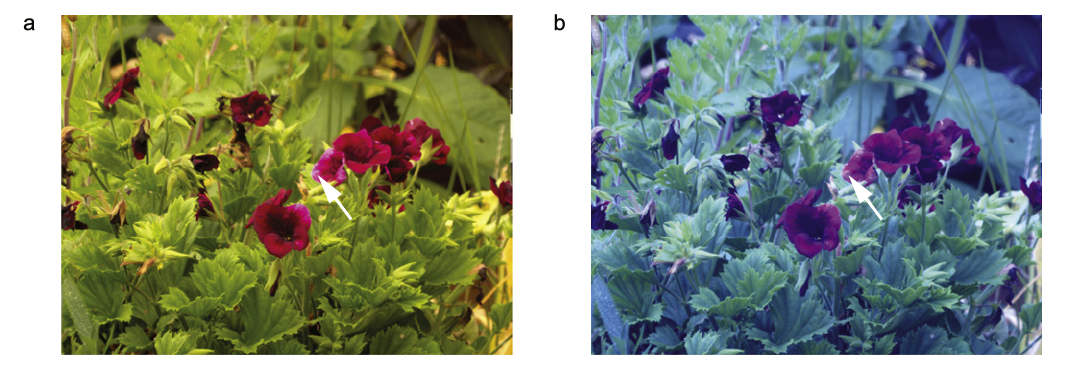
\includegraphics[max width=\textwidth]{figs/LitRev/fosterflowers.png}
% \caption{A single scene under two illuminants (\Gls{CCT} = 4000k and 25000K), reproduced from \citet{foster_color_2011}.}
% \label{fig:fosterflowers}
% \end{figure}

% \begin{figure}[htbp]
% 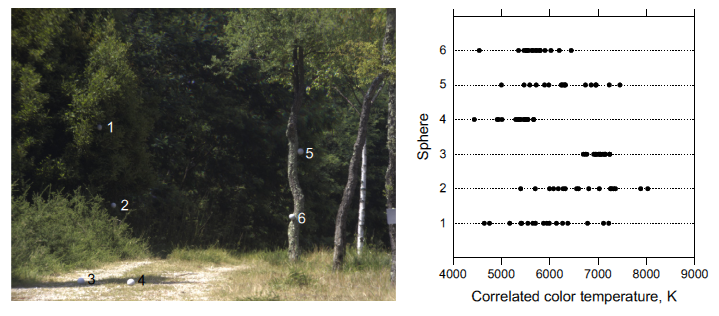
\includegraphics[max width=\textwidth]{figs/LitRev/greyballs.png}
% \caption{Reproduced from \citet{nascimento_spatial_2014}. Original figure caption: ``The color rendition on the left shows the scene with six embedded probe spheres indicated by numbers. The dot plot [on the right] shows the distribution of the CCTs of the local illumination at the 17 sample points on each of the spheres.''}
% \label{fig:greyballs}
% \end{figure}

%Figure \ref{fig:greyballs} gives an indication of the extent to which an object (or more precisely in this case, a group of nominally identical objects) can have varying colorimetric attributes across relatively minor spatial variation. 
%KC: This reads oddly to me, as it's more the illuminance that's varying than the object (if I've understood?).  I'd rephrase this.

% \begin{figure}[htbp]
% \includegraphics[max width=\textwidth]{figs/LitRev/X.png}
% \caption{\hl{Figure showing variation over time.}}
% \label{fig:X}
% \end{figure}

% Figure \ref{fig:fosterflowers} shows a single scene under illumination of two different \glspl{CCT}. The appearance of the object under the two illuminants is likely to have remained somewhat stable to an observer within the real scene, with observers choosing similar colour names for the object under each condition\footnote{Of course the appearance here, with these two images side-by-side, highlights the differences between the two conditions, and shows that under a single state of adaptation there is a clear distinction.}. 


% \subsubsection{Can chromatic adaptation fully account for colour constancy?}

% It may at first appear as though chromatic adaptation may be able to fully account for colour constancy

% RGB heuristic
% yes - cornsweet
% mechanistic vs inferential


% A similar level of variation occurs across time, for example as the sun passes behind a cloud.

% And so we have the central problem of colour constancy and chromatic adaptation: objects of which we have stable colour perceptions are able to be variant in both radiometric and colorimetric attributes without losing their apparent stability. The study of colour constancy aims to answer many questions which revolve around this central conundrum.

% Traditionally %(pre-1986, when \citet{arend_simultaneous_1986} performed what \citet{foster_color_2011} refers to as `the first systematic behavioral experiments' on color constancy) 
% there have existed two stances regards the nature of colour constancy; one held that it was enabled by adaptation of the sensory system, and the other that it was the result of unconscious inference. %KC: citation required
% It is my understanding that whilst great progress has been made in the intervening three decades, this is still a central question, although it appears to be widely accepted that the two frameworks might be complementary rather than mutually exclusive. %KC: citation required

%The best justification for their separation is perhaps that success in their study might serve different aims. 
%The first, the prediction of colour appearance, serves to further the utility of colour science, in particular colour appearance modelling, and the other systems which rely upon colour appearance modelling, such as colour difference formulation. 
%The second is best considered a vision science problem, concerned as it is with the function of the human visual organ, and advancement might endow us with an extension in our understanding of the human body. This in turn would have benefit in multiple areas, including feeding back to the prior aim, for once we understand the underlying mechanics we stand a much better chance of creating robust predictors of colour appearance. 
%Of particular interest to this author, understanding the underlying mechanisms of colour constancy should allow for a more intelligent design of lighting for the spaces which we inhabit, considering that artificial lighting need only resemble natural lighting to the extent that the visual system treats it as similar enough. Creating a colorimetric match to a specific spectra such as D65 is relatively easy, but until chromatic adaptation is more thoroughly understood it is not necessarily entirely clear what the appearance of such a match, or objects illuminated by it, might be. 

%The investigation of \glspl{CAT} generally occurs through the fitting of algorithms to data of corresponding colours, collected in varying manners, such that corresponding colours might be predicted for specific situations. The principal divides between the types of \gls{CAT} tend to hinge upon the method used to collect the data. \citet{nayatani_development_2006} divides the set as those derived from chromatic adaptation theory and those derived from fitting to experimental data, whereas Luo44 makes the divide between those studies based on aperture based experimental procedures and non-aperture based experimental procedures (which generally incorporate more complex, and therefore arguably more realistic, stimuli). Both parties use the terms `CAT Type I/II' to refer to these distinctions, but it is not entirely clear whether their distinctions are complementary. 

% This duality %get rid of this bollocks
% is mirrored by Foster37 in his discussion of the experimental methods employed in colour constancy research where he describes fundamental differences between those experiments which probe chromatic adaptation by asking observers to make `paper matches' (make it look like these two patches were cut from the same sheet of paper) and h/s/b matches (where observers are asked to match appearance in a non-relational manner, that is to match the qualia of a stimuli). This duality occurs again in Foster's37 comparison of relational and non-relational colour constancy, where relational refers to the maintaining of colour relationships in a scene and non-relational again refers to abstracted stimuli qualia). It is my suspicion that all of these disparate dualities are representations of the fundamental duality considered at the beginning of this chapter; that of a distinction between sensory adaptation and inferential computation.

\subsection{Experimental Methods for Colour Constancy Research}

A large range of experimental methods have been used to investigate the problem of colour constancy, partly because different experimenters were approaching the problem from different angles aiming to accomplish subtly separate goals.
Those approaching from a mathematical angle (perhaps with the mind-set `if we find the algorithm which predicts corresponding colours a- this is very useful for industry and b- we can then work backwards to explain how human colour constancy may occur') are concerned primarily with producing chromatic adaptation transforms.
Those approaching colour constancy with a basic interest in the physiology and general function of colour constancy have adopted/created a rather wider set of experimental techniques, owing to the fact that this direction of study is much less well defined than the former, and is at a more exploratory stage of its development.
The \gls{CIE} TC 1-52 report (\gls{CIE} 160:200442) includes an interesting note on the distinction between these two broad approaches; an appendix discusses the reasons why a concerted recommendation was not reached by the group lists the principal factor being a distinction between perspectives as described above. 
\gls{CIE} TC 1-5242 and Luo44 provide a comprehensive overview of the different methods which have been used by the CAT group:
1.	Haploscopic matching
2.	Local Adaptation Matching
3.	Memory Matching
4.	Magnitude Estimation
Haploscopic Matching is the most common technique in this field, and the term refers to experiments which differentially adapt the two eyes and allow an observer to vary attributes of the stimulus presented to one eye such that it in some way matches the attributes of a fixed stimulus shown to another eye. Whilst this is in many ways unnatural, the benefits are that an experiment can be set up so that there is no time interference (the presentations are simultaneous, so memory effects are avoided) and that high precision of match is relatively easily achieved. As assumption is made that the adaptation of each eye is independent.
 
Figure 11 From42.
Local Adaptation Matching can be considered as a variation of haploscopic matching where instead of differing adaptational stimuli being presented to each eye, differing adaptational stimuli are presented to different parts of the same eye (spatially distinct areas of the same retina). The assumption here is that there is minimal intra-retinal interaction. MacAdam's 1956 study49 epitomises this technique. This experimental technique requires that observers minimise eye movement, in order to maintain spatially distinct adaptation.
Memory Matching has traditionally been performed by training observers to communicate colour sensation through the munsell system notation50,51, and then asking observers adapted to different ambient lighting to describe set real objects using such notation. This technique is not much used due to many limitations and confounding factors. Luo44 details the limitations  of this experimental technique succinctly: `a substantial training period being required, complicated procedures for data analysis, lower precision than that of haploscopic technique, limited capacity for retaining information, and memory distortion.'
Magnitude Estimation appears to be similar to memory matching, in that observers are requested to verbally describe an object whilst in an ambient adapting field. The distinction is that the observers are requested to communicate their perceptions using the perceptually meaningful attributes of hue, saturation and brightness, and as such results can be easily integrated into colour appearance models. Recent experiments52,53,54,55,56,57 collected data which was used to create CIECAM97s.
Away from the development of CATs, a subtly different set of experimental techniques has been developed with which to probe the operation of colour constancy. An admirable overview is provided by Foster37:
1.	Asymmetric Matching
2.	Colour Naming
3.	Achromatic Adjustment
4.	Discriminating Illuminant Changes from Reflectance Changes
Asymmetric matching is in many ways synonymous to the haploscopic matching described above and by in \gls{CIE} 160:200442, in that it describes an experimental set-up whereby one stimuli is compared with another, generally where each stimuli exists within a distinct adapting field and attributes of one stimuli can be either adjusted or responded to by an observer. The term asymmetric matching might be thought to be inclusive of a wider range of experimental set-ups, where haploscopic (Greek roots: haploieides, single and skopeo, to view) is necessarily concerned with each individual eye receiving distinct input. Asymmetric matching may refer to experiments where stimuli are viewed simultaneously, successively, or in an alternating fashion, binocularly or haploscopically.
Colour Naming is a technique employed with the aim being a more natural task than  asymmetric matching, and removing some of the `instruction effects' probed by Arend and Reeves40. Foster argues37 that colour naming represents a task apt to measure colour constancy more directly, as opposed to the `relational colour constancy' often studied in asymmetric matching experiments, since it concerns identification rather than equivalence. One clear benefit seems to be that the observer needn't be aware of the equivalence; it is expected that in such experiments there will be only one stimulus, perhaps with a temporally variant adapting field. An observer is simply asked to name colours, and this should theoretically result in a measure of adaptational colour constancy as opposed to inferential colour constancy, so long as the stimuli is suitably abstract . Colour names may be of a fixed set, or an observer may be given free choice. Analysis of results can employ a naming centroid based approach or a boundary focused approach. Speigle and Brainard58 proposed a novel approach combining magnitude estimation and colour naming with the aim to improve precision of response.
Achromatic Adjustment experiments ask an observer to in some way set a stimulus to a neutral achromatic tone, on the assumption that the internal grey point of an observer shifts in response to different adapting fields. These adjustments are generally easy for an observer to make, but the extrapolation of the results makes various assumptions about conceptual colour space and the nature of achromacy. Experiments are easily confounded by complex or real stimuli where there exists a close-to-neutral object in the scene which could consciously or unconsciously be used as a reference.
Discriminating illuminant changes from reflectance changes provides a key way to examine colour constancy in an operational manner. Following the assumption that chromatic adaptation allows an observer to discount the illuminant in some manner, an experimental set up where observers are requested to distinguish between an illuminant change and a reflectance change represents a situation which very closely mirrors the natural process of colour constancy. This experimental technique is well placed to examine whether or not colour constancy in this form is active and efficient, but it provides little way of probing the underlying mechanisms of colour constancy.

%recent advances in colour constancy?
% using more realistic stimuli
% the grey edges algo
% the comparison of grey edge and grey world/bright is white



\section{Retinal Architecture}

\subsection{Rods and Cones} 

%\input{peripheral.tex}
\section{Intrinsically Photosensitive Retinal Ganglion Cells (ipRGCs)}

\textit{Recent reviews by \citet{spitschan_melanopsin_2019}, \citet{do_melanopsin_2019}, \citet{graham_melanopsin-expressing_2016}, and \citet{lucas_melanopsin_2015} provide authoritative overviews of this rapidly progressing research area. This section shall focus on the subgroup of \glspl{ipRGC} called `M1' \glspl{ipRGC}, since these are the most populous and best understood; for details regarding the other subgroups of \glspl{ipRGC} see \citet{ecker_melanopsin-expressing_2010}.}

\bigskip

Retinal rod and cone cells (of three types, l/m/s) are well established as the primary receptors for human vision, and their connections and properties are relatively well understood. Two modes of vision originate from the retina, one of which is associated with image formation and the other which is considered to be \gls{NIF}, and which influences systems such as circadian rhythm entrainment, pupillary reflex and melatonin release. It was originally thought that rods and cones were the sole inputs to both of these modes of vision \citep{hankins_melanopsin_2008}.

\Glspl{RGC} combine signals from groups of cones and rods and relay these signals via the optic nerve to the lateral geniculate nucleus, which in turn processes and relays them further to the cortex for additional processing, allowing for classical vision of objects, movement and colour. \Glspl{ipRGC} are a sub-class of \glspl{RGC}, which in addition to combining and relaying signals exhibit some intrinsic photosensitivity of their own. 

This intrinsic photosenstivity was only confirmed recently relative to our knowledge of other retinal cell types \citep{qiu_induction_2005}, following a search for a retinal cell type or combination of cell types which would fit the spectral sensitivity properties found to influence entrainment of the circadian rhythm in humans and other animals \citep{brainard_human_2001,brainard_action_2001}, which was dissimilar to all of the spectral sensitivities of the cell classes known at the time.

Additionally, it was found that animals and humans with no functioning rods or cones were still able to have a correctly functioning circadian system \citep{freedman_regulation_1999,zaidi_short-wavelength_2007}, further suggesting that that the circadian rhythm was influenced by a novel receptor with a distinct photoreceptor. It is now believed to be these cells which provide the primary input to the \gls{NIF} pathway.

\Glspl{ipRGC} were found to express a photopigment fitting such attributes, and it was given the name `melanopsin'. The spectral sensitivity of melanopsin peaks at around 480nm \citep{qiu_induction_2005,hankins_primary_2002,dacey_melanopsin-expressing_2005,peirson_melanopsin_2006,bailes_human_2013} which places it between the s-cone (cyanolabe photopsin) and rod cell (rhodopic rhodopsin) spectral sensitivities, see Figure \ref{fig:specsens}. In humans, pre-receptoral filtering leads to a functional peak sensitivity of closer to 490nm \citep{cie_cie_2015-1}. 

\begin{figure}[htbp]
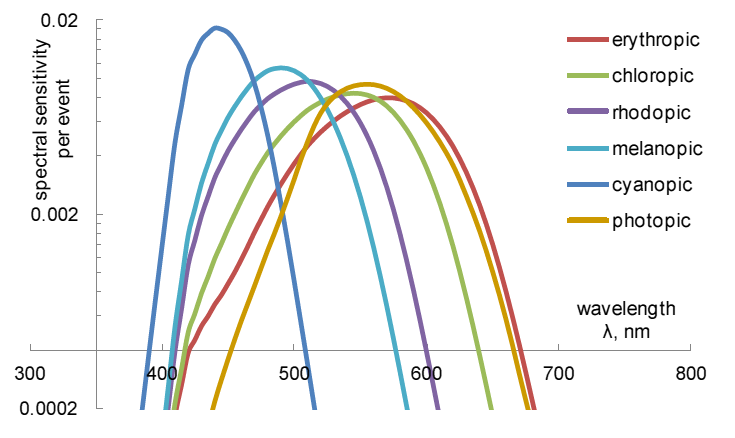
\includegraphics[max width=\textwidth, center]{figs/LitRev/ciemel.png}
\caption{Reproduced from \gls{CIE} TN 003:2015 \citep{cie_cie_2015-1}. \textit{``Spectral sensitivity curves of the five human photopigments to irradiance at the outer surface of the eye of the standard observer and photopic spectral efficiency, normalized to equal area.''}}
\label{fig:specsens}
\end{figure}

Exogenously expressed mouse melanopsin has been shown to be tristable \citep{emanuel_melanopsin_2015,matsuyama_photochemical_2012-1}, that is: existing in one of three possible states. A photon interaction converts melanopsin in one of these states to another, with two of the states being electrically silent (not providing a signal) and one being signal-producing. Notably, these different states have slightly different spectral sensitivities, and thus exposure to specific wavelengths biases the population distribution in different ways, as shown in Figure \ref{fig:melssf}.

\begin{figure}[htbp]
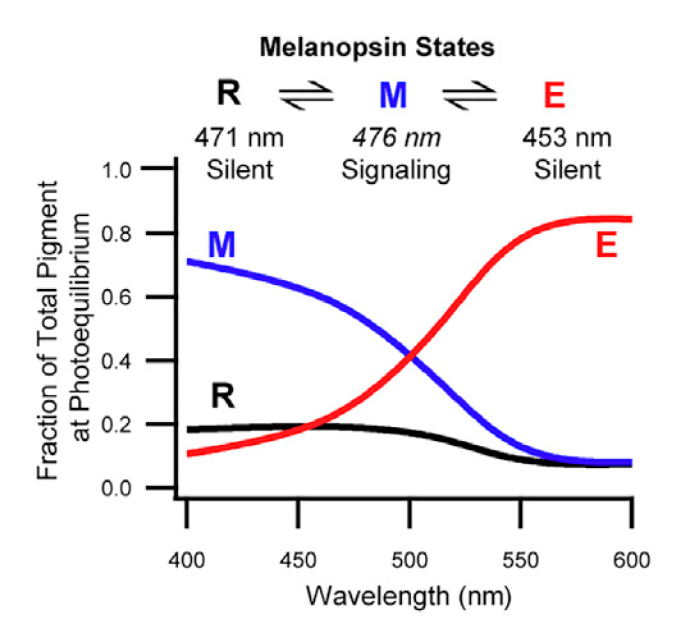
\includegraphics[max width=\textwidth, center]{figs/LitRev/melstates.png}
\caption{Reproduced from \citet{do_melanopsin_2019} (Fig 5D in original source). \textit{``[M]ouse melanopsin is understood to have three states (R, M, and E). The peak spectral sensitivities of R and E are determined from the electrophysiological responses of M1s. Spectrophotometric measurements of purified melanopsin yielded similar values (467 and 446 nm, respectively) and gave information for M (476 nm; [\citet{matsuyama_photochemical_2012-1}]). Bottom, the distribution of melanopsin states as a function of wavelength, estimated from a model based on values from purified melanopsin.''}}
\label{fig:melssf}
\end{figure}

Human melanopsin appears to be bistable (of two states), and there is uncertainty regarding whether this bistability has physiological consequences \citep{cie_cie_2015-1,mure_melanopsin_2009,rollag_does_2008,wada_color_2018,mure_melanopsin-dependent_2007,mawad_absence_2008,koyanagi_cephalochordate_2005,emanuel_melanopsin_2015}. It has been shown in other organisms that colour opponency from a single opsin is possible \citep{wada_color_2018}.

\Glspl{ipRGC} form a sparse mesh across the retina, each covering roughly 10$^{\circ}$ of visual angle \citep{ecker_melanopsin-expressing_2010}; discounting input from other cell types, they operate at a much lower resolution than as would be required for spatial vision of the type we are accustomed to. 

They also operate much more slowly than other cell types, taking several seconds to respond, but are able to sustain a response in contrast to other retinal cell types which are able to respond quickly but only for short periods (See Figure \ref{fig:melspeed} and \citet[p.210]{do_melanopsin_2019} for a summary).

\begin{figure}[htbp]
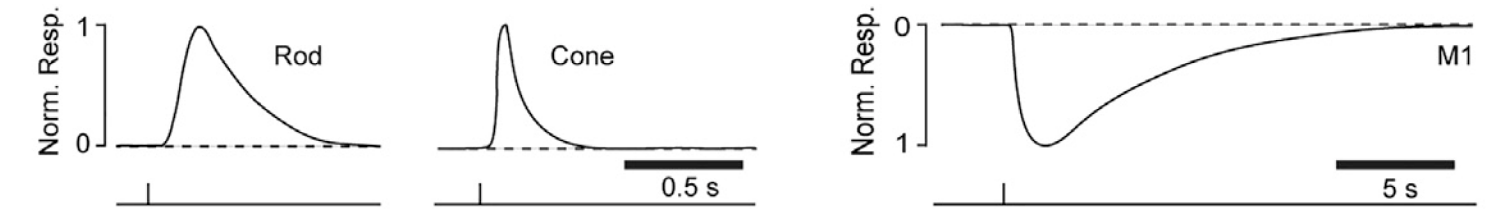
\includegraphics[max width=\textwidth, center]{figs/LitRev/melspeed.png}
\caption{Reproduced from \citet{do_melanopsin_2019} (Fig 5B in original source). \textit{``Dim-flash responses of outer photoreceptors and M1s (normalized photocurrent, having the same waveform as the single-photon response). Note the 10-fold
longer time base for the M1. The dashed line indicates the baseline current and the timing of the flash is shown below the curves, which are traced from
electrophysiological recordings (\citet{emanuel_biophysical_2017,field_nonlinear_2002,nikonov_physiological_2006}).''}}
\label{fig:melspeed}
\end{figure}

\Glspl{ipRGC} vary greatly in the range of light intensities that they are sensitive, are unimodal (stop responding above a certain threshold), and as a population their sensitivity spans a large range of lights levels \citep{do_melanopsin_2019}. It has been proposed that these properties \glspl{ipRGC} would allow an observer to efficiently sense a level of absolute irradiance \citep{brown_melanopsin_2010,milner_population_2017} (restricted to the wavelengths which ipRGCs and their inputs are sensitive to). 

\subsection{Synaptic Input}

In addition to their intrinsic photosensitivity, \glspl{ipRGC} exhibit extrinsic photosensitivity, taking inputs from rod and cone pathways in a similar fashion to regular \glspl{RGC}. Synaptic input is provided by amacrine and bipolar cells (See \citet{belenky_melanopsin_2003} and Figures \ref{fig:lucas} and \ref{fig:do}). 

\begin{figure}[htbp]
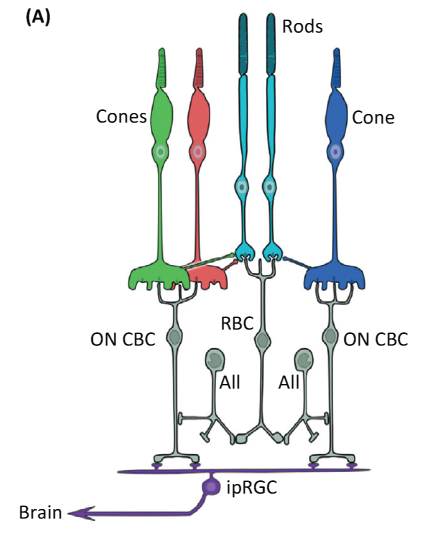
\includegraphics[max width=\textwidth, center]{figs/LitRev/lucas.png}
\caption{Reproduced from \citet{lucas_measuring_2014} (Figure 1A in origial source). \textit{``Schematic of the relevant retinal circuitry in humans. Non-image-forming responses originate in the retina and have been attributed to a particular class of retinal ganglion cell (ipRGC). ipRGCs are directly photosensitive owing to expression of melanopsin, which allows them to respond to light even when isolated from the rest of the retina. In situ they are connected to the outer retinal rod and cone photoreceptors via the conventional retinal circuitry. The details of their intraretinal connections are not completely understood and probably vary between different subtypes. Shown here are major connections with on cone bipolar cells (on CBCs) connecting them to cone and, via amacrine cells (AII) and rod bipolar cells (RBC), rod photoreceptors. As a consequence, the firing pattern of ipRGCs can be influenced by both intrinsic melanopsin photoreception and extrinsic signals originating in rods and each of the spectrally distinct cone classes (shown in red, green, and blue).''}}
\label{fig:lucas}
\end{figure}

\begin{figure}[htbp]
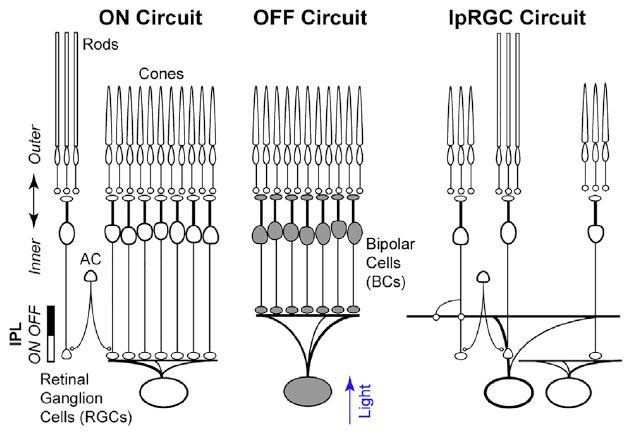
\includegraphics[max width=\textwidth, center]{figs/LitRev/do.png}
\caption{Reproduced from \citet{do_melanopsin_2019} (Fig 1A in original source). \textit{``A highly simplified schematic of the retina in cross-section, oriented with the inner aspect (nearer the center of the eye) down. The outer photoreceptors (i.e., rods/cones) drive bipolar cells (BCs). In the inner plexiform layer (IPL), BCs synapse with retinal ganglion cells (RGCs). Left: ON circuitry. Rods (top) drive rod BCs, whose signals pass through amacrine cells (ACs) to cone BCs. In the inner IPL, ON cone BCs convey signals to ON RGCs. ON RGCs show greater depolarization when light intensity increases. Center, OFF circuitry. In the outer IPL, OFF cone BCs provide synaptic input to OFF RGCs. OFF RGCs show greater depolarization when light intensity decreases. Right: a sample of circuits for outer- and inner-stratifying ipRGCs, which are both ON. ON cone BCs make ectopic synapses with the former and conventional synapses with the latter. Rod pathways also drive ipRGCs. IpRGCs make chemical and electrical synapses with ACs (not shown).''}}
\label{fig:do}
\end{figure}

Inputs evoke ON responses, despite originating from both the ON and OFF layers of the inner plexiform layer (see Figure \ref{fig:do}). \citet{graham_melanopsin-expressing_2016} describe the processes which allow this to occur: 

\begin{itquote}{}
ON bipolar cells use two unconventional strategies to release glutamate onto the dendrites of SCN-projecting mouse ipRGCs in the “OFF” sublamina. Some ON bipolar cells’ axons extend lateral protrusions that contain synaptic vesicles [...], whereas others possess en passant (in passing) synaptic vesicles within their axonal shafts [\citet{dumitrescu_ectopic_2009}]. Distally stratifying ipRGCs are also present in rabbit, marmoset and macaque retinas, and they likewise receive unconventional ON bipolar input in the “OFF” sublamina [...] [\citet{hoshi_inputs_2009}, \citet{grunert_bipolar_2011}].
\end{itquote}

Signals from rods and cones retain their traditional time courses; \glspl{ipRGC} are not inherently sluggish, rather the melanopic inputs to \glspl{ipRGC} are. This can be seen in Figure \ref{fig:wong}, where standard outputs of an \gls{ipRGC} are shown on the left, and outputs with rod/cone driven synaptic inputs blocked are shown on the right. The response is shown to be relatively instantaneous for the cell with intact inputs, but lagging by several seconds for the cell relying on melanoptic activation alone.

\begin{figure}[htbp]
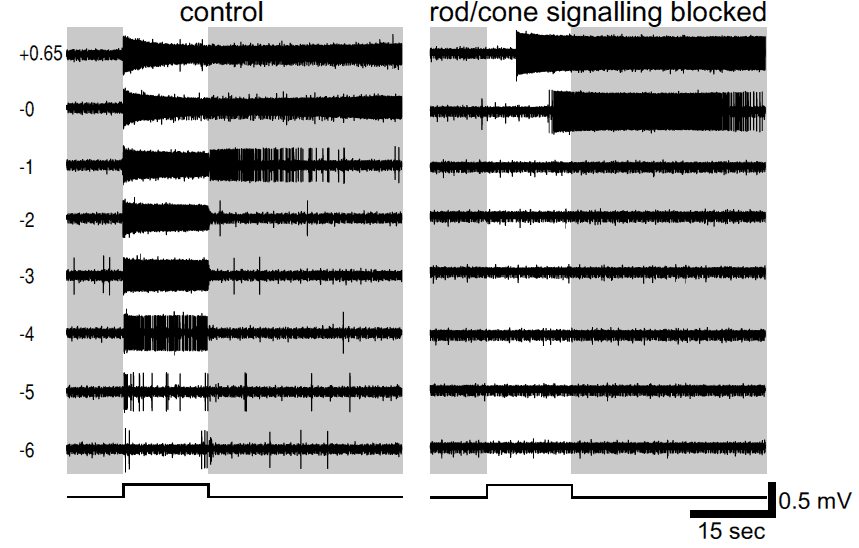
\includegraphics[max width=\textwidth, center]{figs/LitRev/wong.png}
\caption{Reproduced from \citet{wong_synaptic_2007} (Fig 4 in original source). \textit{``Multi-electrode array (MEA) recordings of synaptically mediated light responses in ipRGCs. Extracellular recordings comparing spike responses of an ipRGC to light of various intensities with rod/cone-driven synaptic inputs left intact (left) or blocked (right). Log stimulus attenuation is indicated to the left. Note that all responses to weaker stimuli (-2 log attenuation and dimmer) and short-latency responses to brighter ones (-1 to +0.65 log I) were dependent on synaptic transmission, presumably because they reflect rod and/or cone influence on the recorded cell. Note also that intensities sufficient to recruit the intrinsic response (-0 and +0.65 log I; right) evoke responses with substantial poststimulus persistence, a well-established feature of melanopsin-dependent light responses.''}}
\label{fig:wong}
\end{figure}

There also evidence for \glspl{ipRGC} having intraretinal retrograde synaptic output (\citet{zhang_intraretinal_2008,zhang_melanopsin_2012}, summarised by \citet{graham_melanopsin-expressing_2016}), via a subpopulation of dopaminergic amacrine cells. This type of signalling could provide a feedback loop which modifies signals before they have left the retina.

\subsection{Projection}

\glspl{ipRGC} have been shown to innervate `dozens of brain areas' \citep{do_melanopsin_2019}, with M1s principally innervating \gls{NIF} areas, but with some activation of areas traditionally thought of as image-forming. There appear to be meaningful differences between the different sub-types of \gls{ipRGC} in this respect, with different sub-types (denoted M1-6, distinguished by their retinal morphology) showing distinct activation pathways. 

A summary of these projections is shown in Figure \ref{fig:projection}. From this figure it can be seen that there are still many potential projections which have not been investigated (``Each blue dot indicates the approximate density of innervation by its size, a white dot indicates undetectable innervation, and lack of a dot indicates an absence of information.''). However, it can clearly be seen that outputs are extensive and varied.

\begin{figure}[htbp]
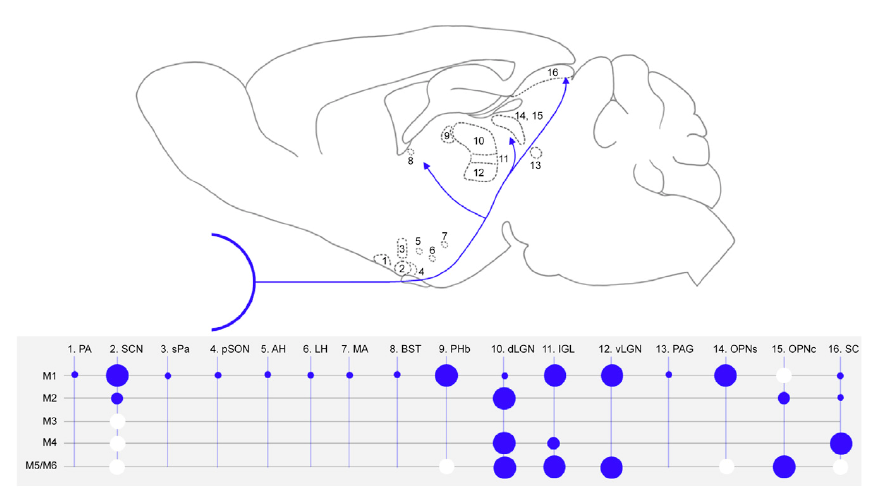
\includegraphics[max width=\textwidth, center]{figs/LitRev/projection.png}
\caption{Reproduced from \citet{do_melanopsin_2019} (Fig 3 in original source). \textit{``Major Brain Targets of Mouse IpRGCs. A sample of ipRGC brain targets is depicted in a quasi-sagittal schematic of the mouse brain. Below is a plot of innervation densities across ipRGC types, drawn after Berson and colleagues (\citet{quattrochi_m6_2019}) and incorporating additional information (\citet{ecker_melanopsin-expressing_2010}; \citet{hattar_central_2006}; \citet{huang_visual_2019}; \citet{morin_retinofugal_2014}; \citet{zhao_photoresponse_2014}). Each blue dot indicates the approximate density of innervation by its size, a white dot indicates undetectable innervation, and lack of a dot indicates an absence of information. M5s and M6s are pooled because their projections were examined together for technical reasons. AH, anterior hypothalamus; BST, bed nucleus of the stria terminalis; dLGN, dorsal lateral geniculate nucleus; IGL, intergeniculate leaflet; LH, lateral hypothalamus; MA, medial amygdala; OPN, olivary pretectal nucleus (with shell, s, and core, c, regions); PA, preoptic area, which includes the VLPO (ventrolateral preoptic area); PAG, periaqueductal gray; PHb, perihabenular zone; pSON, peri-supraoptic nucleus; SC, superior colliculus; SCN, suprachiasmatic nucleus; sPa, subparaventricular zone; and vLGN, ventral lateral geniculate nucleus.''}}
\label{fig:projection}
\end{figure}

\subsection{The roles of ipRGCs beyond circadian entrainment}
\label{sec:ipRGCbeyond}

In recent years there has been a number of publications examining the role of melanopsin outside of \gls{NIF} vision, challenging some of the assumptions about the roles of the signals originating from \glspl{ipRGC}.

A number of studies have found that the signals from ipRGCs are capable of encoding spatial structure \citep{ecker_melanopsin-expressing_2010, mouland_responses_2017, allen_melanopsin_2017, allen_form_2019, zhao_photoresponse_2014}\footnote{For commentary see \citet{spitschan_vision_2017} and \citet{sonoda_re-evaluating_2016}.}, and others have probed the influence upon brightness perception \citep{zele_cone_2018,brown_melanopsin-based_2012}.

Additionally, several researchers have investigated whether \glspl{ipRGC} may play a role in chromatic vision \citep{cao_evidence_2018, spitschan_human_2017-1,zele_melanopsin_2018,horiguchi_human_2013,vincent_adaptation_2019,vincent_adaptation_2019-1}, using the silent substitution paradigm \citep{estevez_silent_1982,spitschan_method_2018}\footnote{Though see \citet{kamar_silent-substitution_2019}.}. These studies are summarised below.

\textbf{\citet{spitschan_human_2017-1}} found an fMRI response in primary visual cortex for each of four participants, in contradiction to an earlier study by the same group \citep{spitschan_human_2016}\footnote{``we now regard our prior study as not fully resolving the possibility that rapid modulation of the ipRGCs drives a cortical response'' \citep{spitschan_human_2017-1}}. Participants reported a visual percept which was ``unpleasant, blurry, minimal brightening that quickly faded''. There was also some evidence of a chromatic percept: ``Many of the subjects described the melanopsin stimulus pulse as being colored. This was typically a yellow–orange appearance, although three subjects reported a greenish percept''.


\textbf{\citet{cao_evidence_2018}} found that ``changing melanopsin activation levels shifts the equilibrium point in the chromatic pathways'', though curiously the effect was only present for the L/(L+M) pathway. The key figure from this study is reproduced in Figure \ref{fig:cao}. 

The authors conclude that melanopsin activation affects the parvocellular pathway to the extent that \gls{ipRGC} activation could be thought of as ``additive to the M-cone signal opposing the L-cone signal in the PC pathway [i.e., L - (M + I)] (where ``I'' for melanopsin activation in ipRGCs) to signal greenness and/or blueness''. 

The authors note that this corresponds to an earlier result from one of the same authors \citep{barrionuevo_contributions_2014} where such a contribution set was proposed. However, the earlier result includes rod contributions, and the specific pathway which they must be referring to is only the 5th component accounting for $<0.01\%$ of the variance in the signals under examination. Meanwhile, no evidence is found for the 2nd component from that same analysis (labelled as konioncellular, representing $1.56\%$ of variance), which they also proposed would have a considerable melanopic contribution contribution. They neglect to mention this in the later paper.

\begin{figure}[htbp]
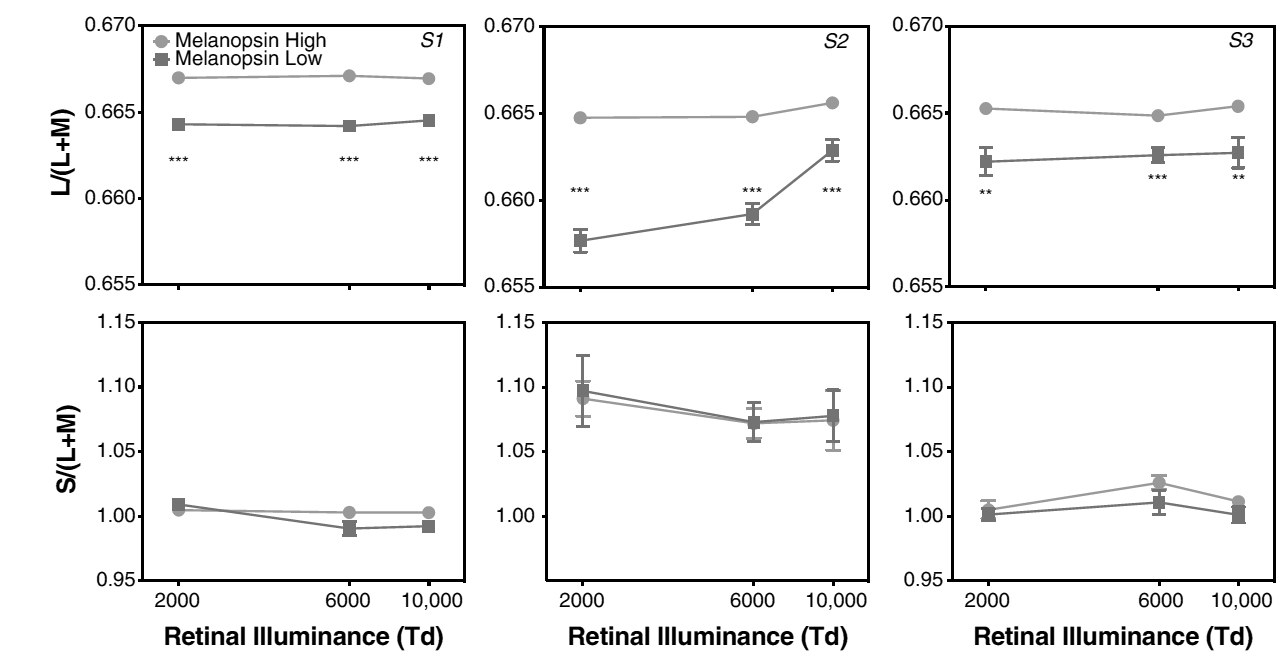
\includegraphics[max width=\textwidth, center]{figs/LitRev/cao.png}
\caption{Reproduced from \citet{cao_evidence_2018} (Figure 1 in original source). \textit{``Unique white $l$ (top) and $s$ (bottom) values (mean $\pm$ sem)
as a function of retinal illuminance for three observers. **$p < 0.01$;
***$p < 0.001$ from t-tests.''}}
\label{fig:cao}
\end{figure}

\textbf{\citet{zele_melanopsin_2018}} found evidence that ``putative melanopsin-mediated image-forming vision corresponds to an opponent S-OFF L+M-ON response property, with an average temporal resolution up to approximately 5 Hz, and $>$10x higher thresholds than red-green colour vision''. The key figure from this study is reproduced in Figure \ref{fig:zele}. This figure shows the perceptual matches to melanopic contrasts in terms of equivalent cone contrasts, for four observers, under three different conditions. For each observer, and for each condition, it can be seen that a melanopic contrast can be matched by an L+M increment and a S/(L+M) decrement.

\begin{figure}[htbp]
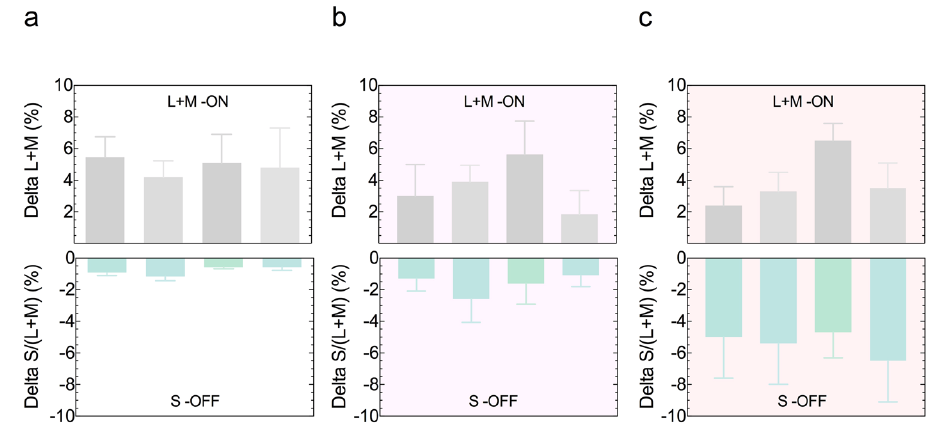
\includegraphics[max width=\textwidth, center]{figs/LitRev/zele.png}
\caption{Reproduced from \citet{zele_melanopsin_2018}. \textit{``Melanopsin photoreception is analogous to an increment in cone luminance [L + M] and a decrement in S-cone excitation [S/(L + M)] with white (a), yellowish-pink (b) and orange adapting stimulus fields (c). [...] Data in each panel are for four participants (mean $\pm$ SEM) measured at 2000 photopic Td.''}}
\label{fig:zele}
\end{figure}

This appears to be a perfect contradiction to the results of \citet{cao_evidence_2018}: \citet{cao_evidence_2018} found a parvocellular response and no koniocellular response whilst \citet{zele_melanopsin_2018} found a koniocellular response\footnote{Albeit inverted: S-OFF L+M-ON, rather than the traditional S-ON L+M-OFF \citep{hendry_koniocellular_2000}.} and no parvocellular response\footnote{Though the matching values for this pathway aren't actually reported. One assumes they did not exhibit a trend and/or fell below some meaningful threshold.}. However, attention should be paid to the distinctions in experimental goals and procedures. \citet{cao_evidence_2018} probe the long term adaptive effects of differing levels of melanopic activation upon white settings, whereas \citet{zele_melanopsin_2019} probe the equivalent appearance of melanopsin in terms of cone-based percepts. It is possible that this distinction is the root of the inconsistency.

\textbf{\citet{horiguchi_human_2013}} found that ``[i]n the periphery, at high photopic levels, human sensitivity is not accurately explained by absorptions in only three types of cone photopigments [and requires a fourth]''. This work focuses on discrimination thresholds rather than attempting to understand a direct perceptual correlate to melanopic stimulation. They conclude that ``[t]he most likely hypothesis is that in healthy human subjects melanopsin absorptions influence visibility.''

Very recent results from \textbf{\citet{vincent_adaptation_2019,vincent_adaptation_2019-1}} report that, contrary to expectations (based on the work of \citet{allen_melanopsin-driven_2014}), ``sensitivity to flicker directed at the cones was not altered by adaptation to a steady field of substantially higher melanopic content''. This appears to rule out the hypothesis that melanopsin activation alters gain (aka adaptation) at an early retinal level for cone-based signals.

Though all the above results are exciting, there are a number of methodological and theoretical areas which require development. The standard methodology used in these experiments is that of `silent substitution' \citep{estevez_silent_1982,kamar_silent-substitution_2019,spitschan_method_2018} where careful tuning of the spectrum is used (see the topic of `metameric blacks' \citep{vienot_verriest_2014,cohen_metameric_1982,vienot_domain_2012,vienot_dimensionality_2015}) to generate signals which are only visible to the chosen receptor-type in theory, in this case melanopsin-expressing \glspl{ipRGC}. 

However, due to variability in observer spectral sensitivities, and limits on the level of stimulus control, it is likely that there will be a small amount of unintended stimulation of non-target cell groups. \citet{spitschan_selective_2015} refer to this as `splatter' (``the expected amount of contrast on nominally silenced photoreceptor classes for a given modulation around a given background''). A suggested control condition is to generate contrast for the nominally silenced cell groups at the level predicted from modelling.

A further concern is that horizontal cell feedback, or other intraretinal retrograde signalling, could result in nominally silenced cone populations still producing an output \citep{kamar_silent-substitution_2019}.

\subsection{Value for colour constancy}

\emph{In this section I shall outline the reasoning which suggests to me that there might be value in a melanopic input for attaining colour constancy.}

Existing colour constancy algorithms fundamentally rely on the ability of cone-receptor-based signals to calibrate cone-receptor-based signals. In this context, by \emph{calibrate} I mean  \emph{modify a raw signal in order to exclude unwanted signal, in order to improve the accuracy (and possibly also precision) of target signal measurement} where the \emph{unwanted signal} would be variation in illumination, and the target signal would be either the \gls{SRF} of a surface or some other identifier of the surface.

This general framework suffers from what I refer to as the issue of circularity in self-calibration\footnote{I suspect that this issue has been discussed in other fields but I have been unable to find such discussion as of yet.}. Generally calibration is performed by characterising a sensor through measurement of an object where the ground truth is known (and/or a measurement from a trusted secondary sensor has been made of this object), and adjusting the properties of the sensor (either at the measurement stage or by implementing a post-processing stage) such that a measurement of the known object results in the expected values. In the case outlined above (cone-receptor-based signals calibrating cone-receptor-based signals), there is no ground truth object, and no secondary sensor, and thus calibration in the traditional sense fundamentally cannot be performed.

If only relative signals are of importance (as opposed to absolute value measurements), then an uncalibrated system might achieve satisfactory stability through the use of measurements taken over time or over space from a single sensor.

A melanopic signal could represent a secondary signal, and the properties of \glspl{ipRGC} seem to make them well-suited for making measurements where the ambient illumination is preferentially detected over transient \glspl{SRF}. Particular properties will be discussed below.

If one's goal was to design a sensor which measured the ambient illumination upon a scene (and was only minimally perturbed by surface reflectances) it might be wise to limit both the spatial and temporal resolution relative to sensors which may be best for measuring surfaces, since the lighting on a scene generally operates at spatial and temporal frequencies which are both lower than surface variation within a scene, particularly when the scene is not viewed from a static position but from a constantly changing vantage (such as is the case with human vision, where the observer is moving body, face direction, and gaze direction regularly). It would also be ideal if the secondary sensor was not strongly adaptive, as this would allow for a more concrete relationship between stimuli and response. \Glspl{ipRGC} exhibit all of the above properties.

There are multiple sites at which a melanopsin-based calibration could occur. The synaptic connections to \glspl{ipRGC} from rods and cones could allow a melanopsin-dependent transform to be performed at the \gls{RGC} stage before signals are output. Alternatively, the intraretinal outputs from \glspl{ipRGC} could allow for modification of signals before reception by traditional \glspl{RGC}. Finally, calibration could occur at any higher post-retinal location assuming that melanopic and cone-based signals could be reconstructed at that point.





\clearpage




\subsection{Peripheral vision}


\section{Museum Lighting}

\bigskip

\begin{itquote}{}
Museums and art galleries collect, preserve, and display natural artifacts and/or examples of human achievement and analyze their impact on the world and the universe around us. Effective exhibit lighting must balance exhibition and conservation needs and enrich the museum experience.
\end{itquote}

\begin{flushright}IES RP-30-96 Museum and Art Gallery Lighting: \\A Recommended Practice \citep{ies_ies_1996}\end{flushright}

\bigskip

Lighting in museums is required to satisfy multiple criteria; perhaps the least contestable requirement being that the lighting illuminate objects such that they are suitably visible to museum visitors. Also of utmost importance in most museum settings is that the lighting does not have an unreasonably damaging effect upon the objects or environment, be this through direct photodegradation or as a result of heat transfer. Further to these requirements, an increased or optimal visual quality is generally desirable, although what this represents or how to achieve it is generally ambiguous.

In sweeping terms, all electromagnetic radiation (visible and non-visible) damages objects, and more radiation damages objects proportionally moreso. Thus the question becomes: \emph{how little light can we use to illuminate objects such that they're visible to the extent required?} The inverse form, sometimes used on the assumption that more light always represents an increase in observer satisfaction/pleasure is: \emph{`how much light can we use so that only $x$ damage occurs over $y$ time'}. 

Industry guidance documents provide advice on how to manage lighting to best address the above requirements and many other additional specific requirements through the recommendation of procedure and provision of target figures for quantitative variables. \Gls{UV} radiation, being of no visual benefit but having potential to harm, is now excluded from gallery spaces as an industry standard. %KC: citation required

%KC: I would add a summarising sentence here e.g. "This section discusses existing literature covering the various factors that need to be considered when choosing a museum light source, specifically those that relate to its SPD.  These include the likelihood of damage and the visitor experience.  A discussion of existing museum guidance on these topics is also provided.

\subsection{Damage functions} \label{sec:DamageIndex}

%KC: Can you link this to the ipRGCs?  Overall, this shows that in terms of material damage, the wavelengths to avoid are the low ones and that light sources which have high intensities at the peak sensitivity of melanopsin could be considered as not particularly hazardous for museums.

\textit{The key reference on this subject is \gls{CIE} 157:2004 \citep{cie_cie_2004}, and valuable talks on the subject were given at the recent Museum Lighting Symposium \& Workshops \citep{pokorska_book_2017} (which the author helped to organise), and have been made freely available online\footnote{See in particular the talks by David Saunders (\url{https://www.youtube.com/watch?v=H4d0qH0IBcI&t}) and Stefan Michalski (\url{https://www.youtube.com/watch?v=XUY9biLQqlw}).}}.

\bigskip

In heritage science `damage functions' are ``functions of unacceptable change, dependent on agents of change'' \citep{strlic_damage_2013}. The goal of damage functions in heritage lighting engineering is to give a quantitative means by which to predict the amount of damage caused to a prototypical object by a given light source, and to assist in limiting such damage. They generally follow the logic that radiation of lower wavelength is likely to cause more damage to objects.

\citet{harrison_report_1953} is generally acknowledged as the first to suggest such a function, but he himself acknowledges that it had ``long been established that the shorter the wavelength (visible yellow, green, blue, violet and invisible UV being progressively shorter) the more photochemically potent will be such radiant energy, provided such energy is actually absorbed''. \citet[p.9]{harrison_report_1953} defined the `radiation hazard associated with a light source' as:

\begin{equation}
    \sum_{0}^{\infty} \mathrm{H}_{\lambda} \mathrm{D}_{\lambda} \Delta \lambda / \sum_{0}^{\infty} \mathrm{H}_{\lambda} \overline{\mathrm{y}}_{\lambda} \Delta \lambda
    \label{eq:Harrison}
\end{equation}

where $\mathrm{H}_{\lambda}$ is the spectral irradiance, $\mathrm{D}_{\lambda}$ is the `Relative Damage Factor' (which is extrapolated from the data collected shortly prior to Harrison's own report by the National Bureau of Standards \citep{national_bureau_of_standards_preservation_1951}, and shown in Figure \ref{fig:Harrison}), and $\overline{\mathrm{y}}_{\lambda}$ is the \gls{CIE} 1924 photopic $V_{\lambda}$ luminosity function. The resulting value would describe the amount of damage expected from a light source, normalised by its luminance.

\begin{figure}[htbp]
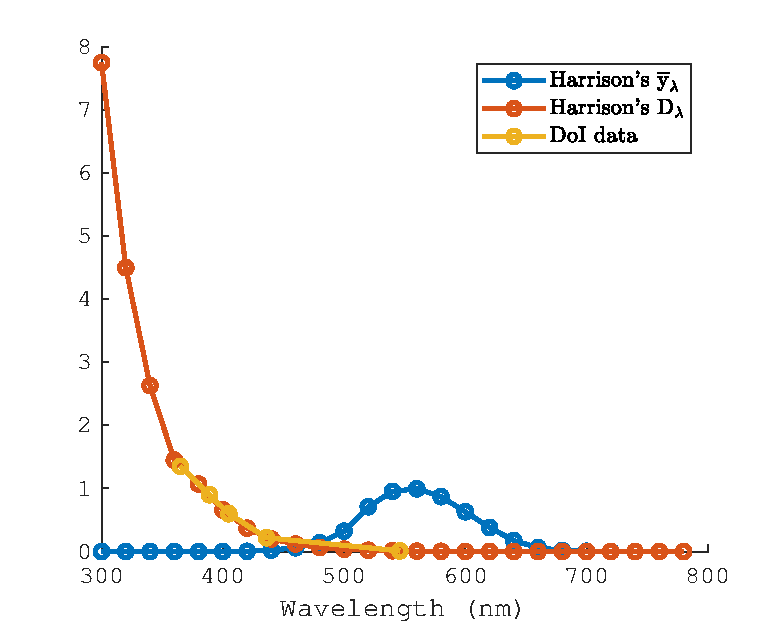
\includegraphics[max width=\textwidth]{figs/LitRev/HarrisonAndDoI.pdf}
\caption{Harrison's \citep{harrison_report_1953} damage function ($\mathrm{D}_{\lambda}$), and luminous efficacy ($\overline{\mathrm{y}}_{\lambda}$), alongside the Declaration of Independence data \citep{national_bureau_of_standards_preservation_1951} from which it was extrapolated (re-normalised to match scale).}
\label{fig:Harrison}
\end{figure}

\begin{figure}[htbp]
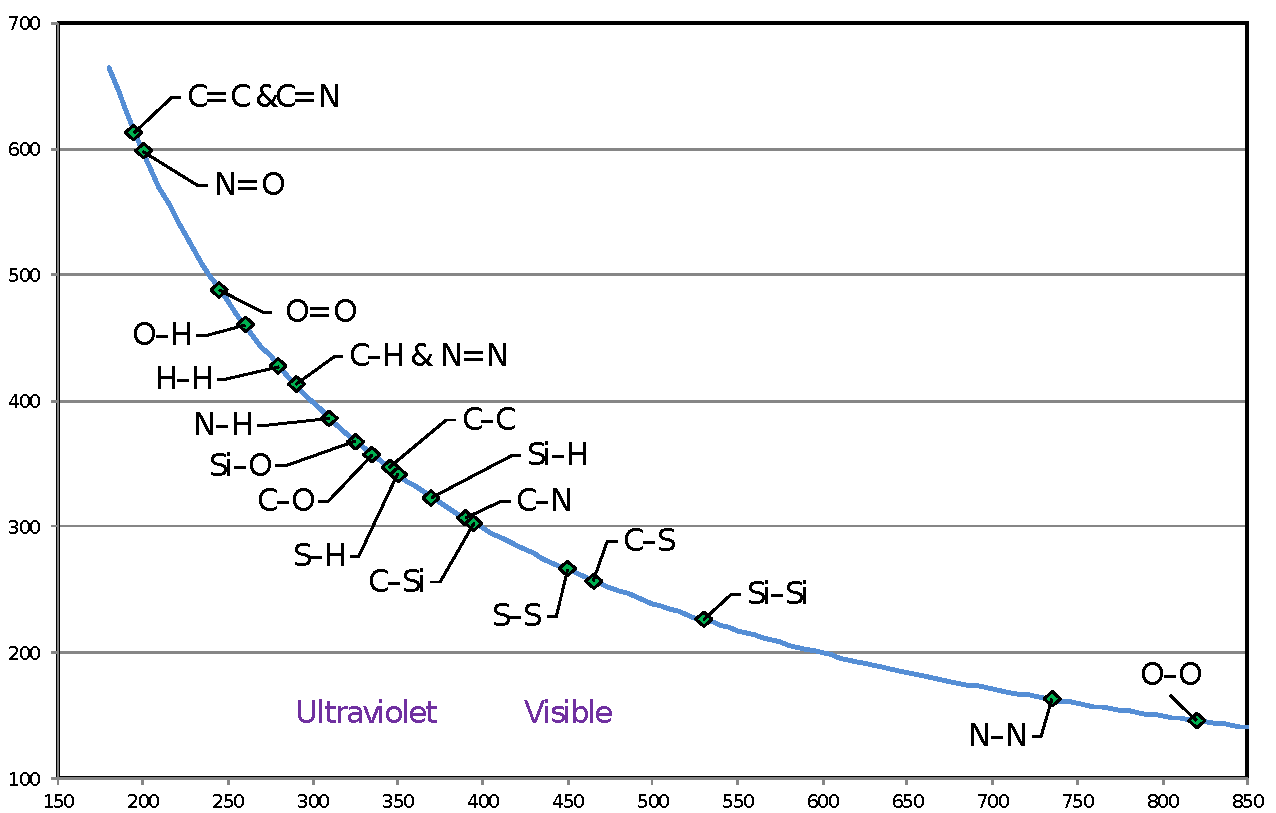
\includegraphics[max width=\textwidth]{figs/LitRev/Saunders.pdf}
\caption{Graph courtesy of David Saunders, presented at the Museum Lighting Symposium \& Workshops \citep[p.61]{pokorska_book_2017} showing the relationship between wavelength and the bonds which can be broken in various molecules, with `Wavelength (nm)' on the abscissa and `Bond energy (kJ/mol)' on the ordinate.}
\label{fig:Saunders}
\end{figure}

There has been extended scepticism about the utility of damage functions in general, with the argument being that no one damage function could represent the vast range and complexities of real materials. \citet[p. 178]{thomson_museum_1978} wrote that ``for more fugitive materials \dots the figure for visible radiation would be higher. On the other hand \dots the fastest dyes are probably affected only by UV. Thus it can be seen that no single figure can be given for damage versus wavelength''.

Criticism was aimed at this specific damage function due to its derivation from such a small and minimally representative dataset - Harrison's data was `extended' from the 5 datapoints measured by the National Bureau of Standards \citep{national_bureau_of_standards_preservation_1951} in their investigations of how to best care for the Declaration of Independence\footnote{It is a curiosity that these minimal figures would not in fact have been much use to those planning the care for the declaration, since in the report it is noted that ``The deterioration of animal parchment is not as rapid as that of the low-grade paper for which the damage factors were determined'' \citep{national_bureau_of_standards_preservation_1951}, and the Declaration of Independence is written on animal parchment.}, and was derived from the study of `low-grade paper', which cannot to said to represent the average museum item\footnote{Though \emph{no} material truly can!}.

\gls{CIE} 157:2004 \citep{cie_cie_2004} notes that whilst Harrison's proposal failed to gain acceptance as the procedure for comparing the damage potential of different types of light sources, it did convince people of the ills of \gls{UV}, with the result that daylight was subsequently eliminated from many galleries.

Following \citet{cuttle_lighting_1988}, who noted that Harrison's damage function could be well fit by an inverted logarithmic function, with parameters controlling the slope and normalisation point of the function, \gls{CIE} 157:2004 provided the following equation:

\begin{equation}
    s(\lambda)_{\mathrm{dm,rel}}=\exp [-b(\lambda-n)]
    \label{eq:damfac}
\end{equation}

where differing values of $b$ for 5 categories of item are provided (Table \ref{tab:b}), $n$ is the normalisation value (\gls{CIE} 157:2004 uses a value of 300), and the $s(\lambda)_{\mathrm{dm,rel}}$ function is the estimated action spectrum for each category. $s(\lambda)_{\mathrm{dm,rel}}$ would be substituted into Equation \ref{eq:Harrison} for $\mathrm{D}_{\lambda}$. \gls{CIE} 157:2004 also provides values of $H_{s,dm}$ which indicate the susceptibility of each group of materials to damage (where damage is considered as colour change%in $\Delta E_{\mathrm{ab}}^{\ast}$
).

\begin{table}[htbp]
\centering
\begin{tabular}{|c|l|l|l|}
\hline
Group & Samples & $H_{s,dm}$ (W h/m$^{2}$) & $b$ \\ \hline
a & Low-grade paper & 5 & 0.038 \\ \hline
b & Rag paper & 1200 & 0.0125 \\ \hline
c & Oil paints on canvas & 850 & 0.0115 \\ \hline
d & Textiles & 290 & 0.0100 \\ \hline
e & Water colours on rag paper & 175 & 0.0115 \\ \hline
\end{tabular}
\caption{Table reproduced from \gls{CIE} 157:2004 \citep{cie_cie_2004}, showing the values for $H_{s,dm}$ and $b$ for various categories. Note: the source for this data is not particularly clear; it is listed as `The Berlin researchers', which is assumed to follow the references: \citet{krochmann_beleuchtung_1988,cie_cie_1991,hilbert_zur_1991}; none of which I have been able to access.}
\label{tab:b}
\end{table}

The more general criticism that damage functions will never be able to represent all museum objects is a valid concern, and can be well illustrated with the following logic: museums own objects of many different colours, different colours arise from different reflectance properties, different reflectance properties mean different wavelengths are absorbed, and damage can only occur when radiation is absorbed. Thus it follows that one would expect two objects of different colours to have different damage functions. 

The classic study on how reflectance properties relate to damage is that of \citet{saunders_wavelength-dependent_1994}. They exposed a number of pigments to a range of wavelengths and measured the resulting damage.%KC: Can you give a bit more detail in this sentence?  Did Saunders and Kirby use a series of monochromatic light sources?  Did damage mean colour change here?
\citet{cuttle_control_1999} later replotted the data from this study (see Figure \ref{fig:Cuttle}), highlighting the apparent joint contributions of spectral reflectance and a general damage function to the individual damage functions. \gls{CIE} 157:2004 notes however that this correspondence is not perfect or easily modellable, and that ``a workable system for characterising action spectra for colorants, including pigments and dyes, remains an unattained goal''. Recent studied have added new data (see esp. \citet{villmann_wavelength_2018}), and it is hoped that a general understanding may at some point be reached.

\begin{figure}[htbp]
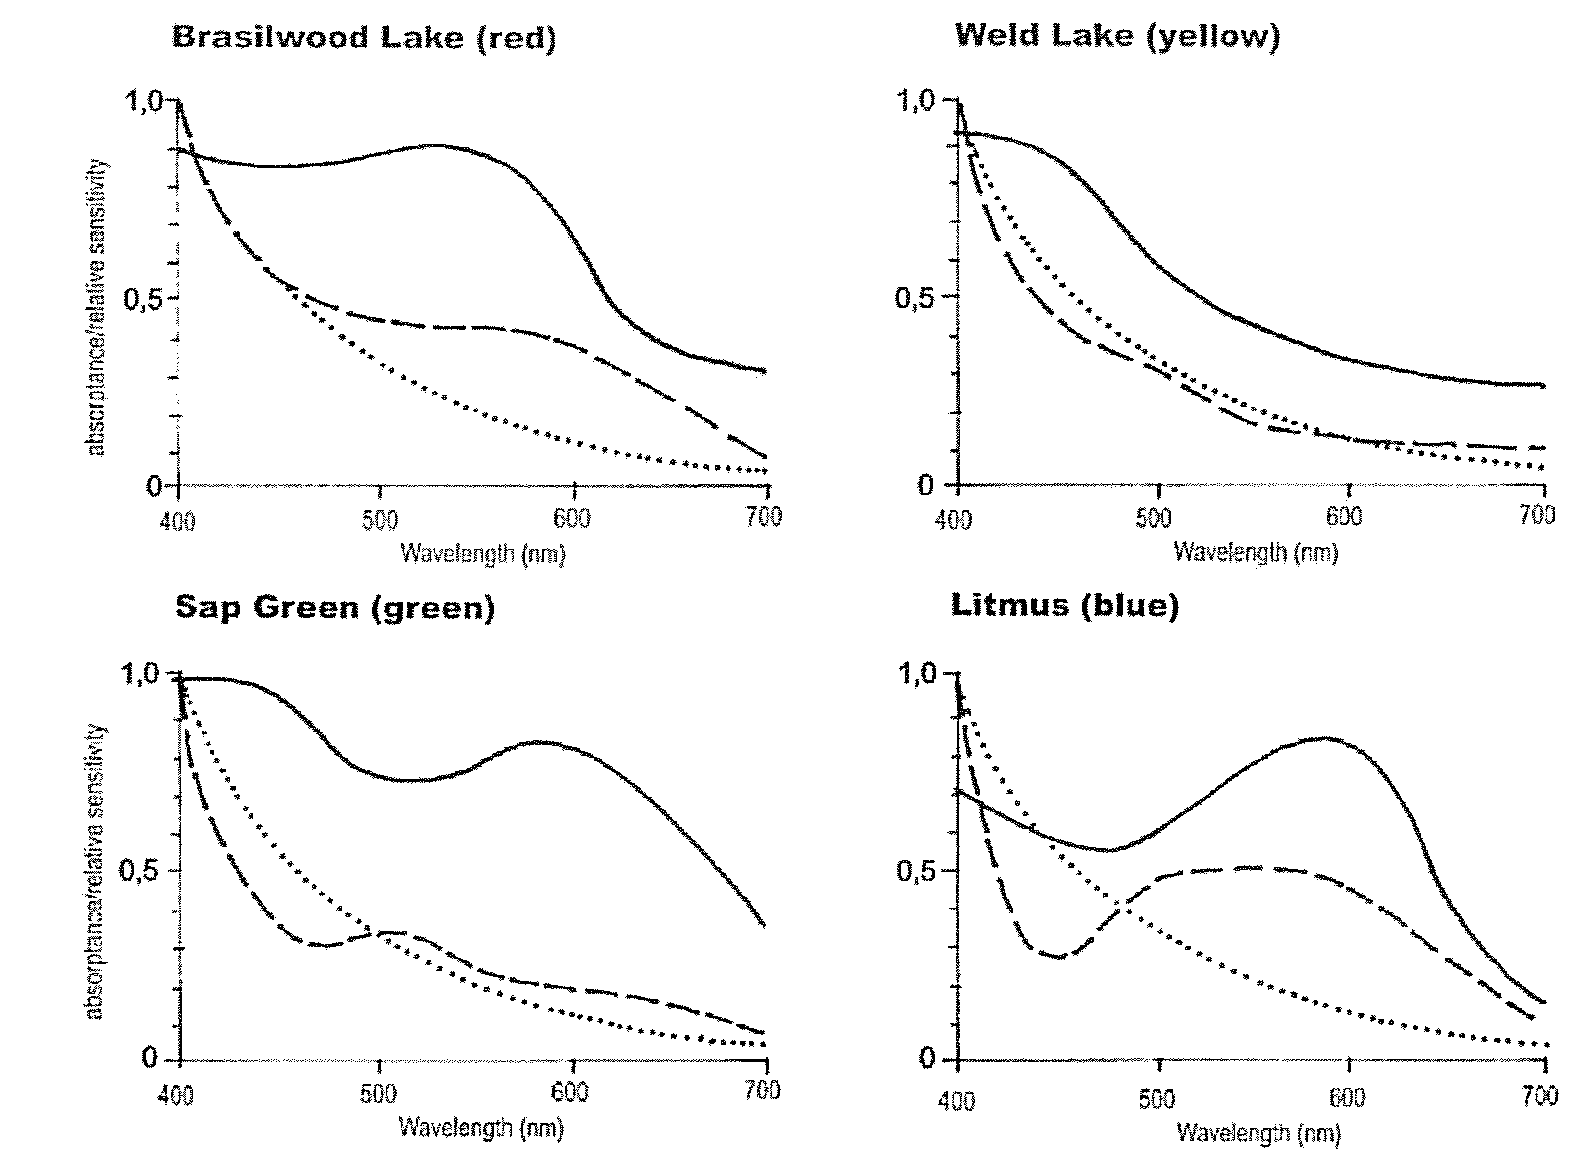
\includegraphics[max width=\textwidth]{figs/LitRev/Cuttle.png}
\caption{The original data for this figure is from \citet{saunders_wavelength-dependent_1994}, later re-plotted by \citet{cuttle_control_1999}, and reproduced (with the addition of the Berlin functions) by the authors of \gls{CIE} 157:2004 \citep{cie_cie_2004}. Caption from \gls{CIE} 157:2004: ``Spectral absorptance (solid line) and relative spectral responsivity (broken line) for artist's pigments \dots The dotted lines show relative spectral sensitivities normalised at 400nm based on the Berlin relative spectral responsivity function.''}
\label{fig:Cuttle}
\end{figure}

However, it is the opinion of this author that this argument is an exercise in artificial futility; whilst we may not be able to model the individual damage functions for every object in a museum, we may at least use one which has some bearing on the damage function, rather than the one which is implicitly used by museums currently - the \gls{CIE} 1924 luminosity function ($\overline{\mathrm{y}}_{\lambda}$ of Figure \ref{fig:Harrison}), which relates to the sensitivity of the human eye rather than any type of object. \citet{cuttle_lighting_1988} puts it well: ``The argument, then, is not whether we have a [damage] function which is correct, but whether we can improve usefully upon the likely reliability of the present system''. It is depressing that this was said in 1988 and yet little seems to have changed in practice (See Chapter \ref{chap:Interviews}).

In the case where specific objects/pigments of interest can be identified, and their individual damage functions calculated, there is valuable research to draw on regarding methods for optimising light sources to minimise damage, initiated by \citet{miller_evaluating_1993} and developed by many others \citep{durmus_optimising_2017,durmus_colour_2015,durmus_optimising_2015,durmus_object_2017,delgado_ramos_art_2009,delgado_lighting_2011,luna_selective_2015,cuttle_proposal_2000,vazquez_point_2017}. The fading of lead chromate in the paintings of Vincent van Gogh has captured public attention \citep{lewis_smith_will_2013} and has resulted in multiple studies looking at ways to optimise the illuminant for this one particular material \citep{lunz_can_2017,monico_degradation_2011}.

With modern computation, and access to datasets, it becomes relatively easy to calculate a value of \Gls{DI}. Figure \ref{fig:Houser} shows the results for such computations for 401 illuminants and light sources (as per Equation \ref{eq:Harrison}, using a damage factor computed as per Equation \ref{eq:damfac}, but further normalised such that Illuminant A has a reference value of 1)\footnote{The code to reproduce this is available from: \url{https://github.com/da5nsy/DamageIndex}}. It can be seen that whilst most illuminants cluster around 1 there is a broad range. It should be remembered that these illuminants would in no way indicate their relative damage index to an observer or a purchaser, unless one went to the effort to look up or measure the \gls{SPD} and compute the damage factor. A careful or careless choice in this respect could easily double or halve the amount of time an item could be exhibited before succumbing to terminal damage.

\begin{figure}[htbp]
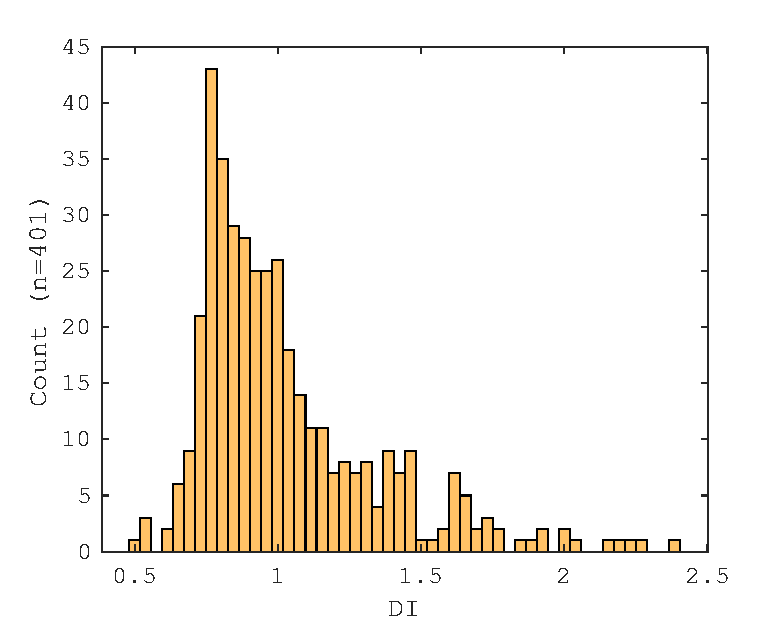
\includegraphics[max width=\textwidth]{figs/LitRev/DI.pdf}
\caption{The values of $DI$ for the 401 illuminants used by \citet{houser_review_2013}, available via \gls{PTB} as `spd\_houser', normalised such that \gls{CIE} Illuminant A receives a reference value of 1.}
\label{fig:Houser}
\end{figure}


\clearpage
\subsection{Visitor Requirements of Museum Lighting}

The visual requirements of museum visitors is likely to depend upon a large number of variables, both intrinsic and extrinsic to the visitor (e.g. intrinsic - age, cultural background, goals for the museum visit and extrinsic: luminance, lighting distribution, \gls{CCT}, \gls{CRI} and flicker properties of lighting). Some of these factors have been independently studied in a museum context, and for others it is likely that findings in other environments could generalise such that they could be used to inform decisions regarding museum lighting.

Traditionally, the principal manner in which museum professionals sought to limit damage was through setting a maximum luminance level. The implicit assumptions in this process are twofold; firstly: that damage will increase with increased luminance. This was a fairer assumption when tungsten was the only type of lighting technology, but as other lighting technologies with different \glspl{SPD} have been introduced this assumption has become less accurate (see Section \ref{sec:DamageIndex}: \nameref{sec:DamageIndex}). The second implicit assumption is that viewers will prefer higher luminance environments.

The classic study on this second assumption, performed in a mock-museum environment is that of \citet{loe_preferred_1982}. This research regards the display of oil and watercolour paintings specifically. In this study Loe et al. examined three variables: painting illuminance, light source (different technologies) and light distribution. Following the construction of a mock up gallery space, observers were asked to view paintings of various types under a range of illuminations, varying in `painting illuminance, light source and light distribution within the gallery space' and report upon semantic scales their perceptions. The results which informed the 200 lux recommendation stem from only the first variable, painting illuminance. Here it was found (as shown in Figure \ref{fig:Loe}) that for factors christened `discrimination' and `quality evaluation' (distilled from factor analysis of the original semantic data) there was `a steep rise in discrimination and quality assessment until and illuminance of approximately 200 lux is reached: above this illuminance the rate of increase in reduced.' This conclusion has had substantial impact in setting guidelines and future thinking was that a minimum of 200 lux was required to `give visual satisfaction', however it can be seen from Figure \ref{fig:Loe} that the data is sparse, noisy, dependent upon brand of illuminant and doesn't show a particularly strong effect of 200 lux in particular. Further, only a small number of different luminances were sampled, and it is quite possible that the results are at the mercy of several types of bias \citep{fotios_research_2009}. This figure was subsequently used in \citet{thomson_museum_1978}, which has informed a great deal of subsequent thinking on the topic.

\begin{figure}[htbp]
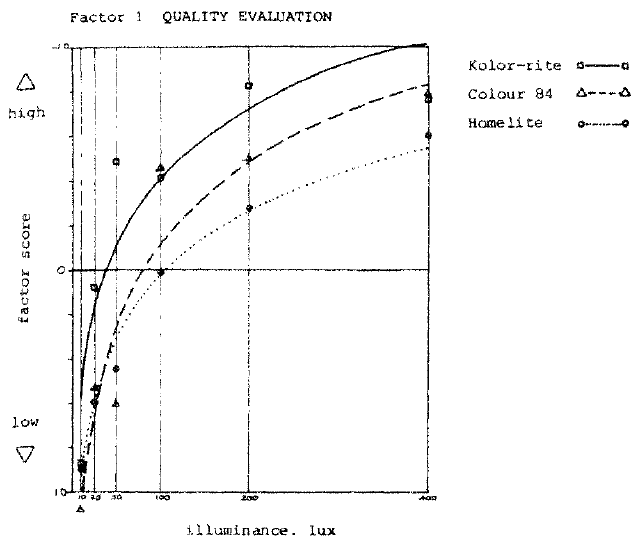
\includegraphics[max width=\textwidth]{figs/LitRev/Loe.png}
\caption{Illuminance vs a factor which is thought to indicate `quality', for three different brands of illuminant, reproduced from \citet{loe_preferred_1982}.}
\label{fig:Loe}
\end{figure}

There has been extensive research on the visitor requirements in terms of \gls{CCT} and \gls{CRI} and these shall be covered in separate sections.

In terms of a holistic approach to museum lighting research (considering more than a single or small number of isolated variables), there has been a great deal of work which deals with the visitor experience in a broad and cultured fashion from the lofty vantage of museum studies (such as \citet{falk_museum_2016} and \citet{shapiro_museum_1990}), but rarely do the physical practicalities such as lighting get a mention. 

The notable exception, where lighting as it relates to the visitor experience is considered, is the work of Kesner in the USA in the early nineteen-nineties \citep{kesner_museum_1993-1,kesner_museum_1993,kesner_exhibition_1992,kesner_current_1991,kesner_analysis_1997}.

Kesner's studies comprised self-reporting surveys, and concluded that colour accuracy was the highest requirement and that `richness' of colour was the lowest priority\footnote{A cautious interpretation of these results is advised, considering that there were high average scores for each category.}:

\begin{citequote}{kesner_museum_1993-1}
Artifact appearance, particularly clarity of artefact form and accuracy of artifact color, is the most important visitor need. Although visual impression, specifically acceptable gallery brightness and rich artefact color, is least important among the factors, it too rated highly important.
\end{citequote}

%more?

%Following the release of guidelines on the topic of \glspl{LED} in museums \citep{druzik_guidelines_2012}, a written survey of museum professionals who had requested these guidelines was performed, and the results reported by \citet{perrin_ssl_2014}. The respondents were predominately based in USA, with 30\% identifying as `international'. The survey was part of the USA government's `GATEWAY program'. Responding to the question `Please rank the following factors in your selection of lamps', joint first priorities are identified as `colour and spectral power distribution' and `damage potential'.

\subsection{Museum Lighting Specification Guidance Documents}

\textit{For a historical perspective on museum lighting guidance see \citet{druzik_museum_2007}.}

Five museum lighting guidance documents, thought to represent the most referred to documents in the field (informed by the interviews reported in Chapter \ref{chap:Interviews}), were reviewed. 

The purposes of this section:
\begin{enumerate}
\item To explore how museum professionals specify lighting, by understanding the tools and guidance which are available
\item To enquire as to what the guidance actually is, in terms of what subjects are covered and what the guidelines actually are
\item To question what these guidelines are based upon. How are the results of scientific study utilised in the production of these documents?
\end{enumerate}

Limiting the damage to museum objects by photodegradation is most often the responsibility of the preventive conservator within a museum, or the person holding a role which encompasses this role in the case of smaller institutions. It is therefore essential that the people in these roles have access to standardised and validated advice on how to approach the subject. Several overviews of the subject have been written and I shall aim to introduce the most prominent here, focusing on their aims, scope and differences/similarities. 

I shall operate a biased interest towards the recommendations regarding colour rendering, colour temperature, and illuminance level. Whilst the first two are the immediate area of study within this project, the third (luminance) is of interest for multiple reasons. Firstly, it is the most prominent area in which lighting guidance is provided, on the assumption that there exists a correlation between illuminance and damage, and secondly because of the unit of specification- lux, which is generated using a function of wavelength designed to provide a correlate of brightness to humans. As a human based function, it is within the scope of interest to this project.

There shall be an active occlusion of any advice, no matter how interesting, pertaining to subjects other than lighting and to areas of lighting guidance which do not fall into the above remit, such as directionality, UV/IR damage, advice relating to specific technologies and areas of discussion such as cost calculations or warranty considerations. 

Firstly, a general note regards the mind-set of those providing recommendations: conservation recommendations provided to museums, which might be presumed to be concerned with a method for limiting damage, are generally in no way informed by the sensitivity of a prototypical object, nor how light might act upon it, but rather it is concerned with maintaining a minimal acceptable light level for an observer to view objects under.

This is based on the argument as follows: all light is damaging, but required in order for visitors to see objects. Damage by light acts in a roughly reciprocal manner, such that a small amount of light over a long time period might be made to do equal damage as a large amount of light over a short period. Considering the multiple aims of museums; (1) to display objects, but also (2) preserve them such that they may be displayed to future generations, it seems desirable to find the minimal amount of light that satisfies the first aim, such that the ability to deliver on the second aim is maximised. Thus many of the recommendations discussed here are actually concerned with the ability of a viewer to extract visual information. This point is not always entirely clear, and it is my suspicion that conservators are sometimes lulled into believing that there is something special about the specific values recommended regards their ability to `avoid' damage. 

One clear exception to this, which will be discussed in further detail, is \gls{CIE} 157:2004 \citep{cie_cie_2004} which considers damage functions of specific materials. These deal specifically with the degradation of objects, with less regard to how objects might appear. Other works which deal with damage functions either generally or for specific types of objects fall into this exception also.

The common language most regularly employed in both of these approaches is the term of 'lux', though this is a contentious issue with some arguing that it correlates well enough with damage potential, and others exploring the use of damage functions. `Lux' relates loosely to the human perception of brightness, but does not consider any type of material absorbance, reflectance or damage function. The historical background to this precedent appears to be as follows; whilst technological ability to vary the spectral power distribution of a light source was limited (whilst tungsten was the dominant source of illumination) is could be assumed that there was a predictable relationship between lux and radiometric spectral power distribution, such that any two lights with the same lux level would cause the same level of damage to any specific object, and thus providing damage minimisation advice could be done using the language of lux, which was pre-established considering the original approach outlined above. This approach is now less appropriate, considering the increased variability in spectral power distribution provided by the introduction of LED technology, and it is reasonable to assume that in the future additional lighting technologies (or variations of existing technologies) might be introduced, with again fundamentally different types of spectral power distribution.

This field may be divided into publications which relay original research, generally in the form of journal articles and conference proceedings, and longer publications which aim to provide an authoritative voice on the subject (often including references to the aforementioned journals). I shall cover principally these longer documents, since my priority interest in this section is the advice which is currently provided and the methods in which this advice is conveyed. The question of how much conservators rely on guidance documents vs referring to ongoing research is an interesting question in of itself, and shall be covered in my discussion of the interviews conducted with current museum professionals (See Chapter \ref{chap:Interviews}).

\noindent
The guidelines chosen for review were:
\begin{itemize}
\item The Museum Environment \citep{thomson_museum_1986}
\item \gls{CIE} 157:2004 Control of Damage to Museum Objects by Optical Radiation \citep{cie_cie_2004}
\item Guidelines for Selecting Solid-State Lighting for Museums \citep{druzik_guidelines_2012}
\item SLL LG8: Lighting for museums and art galleries \citep{cibse_lighting_2015}
\item IES RP-30-96 Museum and Art Gallery Lighting: A Recommended Practice \citep{ies_ies_1996}\footnote{This has since been usurped by IES \citep{illuminating_engineering_society_ies_2017}.}.
\end{itemize}

\noindent
In summary:
\begin{itemize}
\item Recommended values were provided for:
\begin{itemize}
\item \emph{Lux}: various, dependent on sensitivity, generally based on figures from the study of visual preference by \citet{loe_preferred_1982} via \citet{thomson_museum_1978}.
\item \emph{R$_a$}: various, most frequently \textgreater 80, generally with no experimental basis referenced or justification for this exact figure.
\item \emph{\gls{CCT}}: various, based implicitly on \citet{kruithof_tubular_1941} or on such ideas found empirically.
\end{itemize}
\item Most also suggested visual inspection as a valid means of assessment.
\item There was often blurring between recommendations concerned with visual appearance and those concerned with conservation. 
\end{itemize}

\subsubsection{`The Museum Environment'}

`The Museum Environment', first published in 1978 \citep{thomson_museum_1978}, with a popular second edition published in 1986 \citep{thomson_museum_1986} (I shall hereon be referring to this later edition), appears to be one of the most frequently consulted resources on the subject of lighting for practising museum professionals. Whilst the book encompasses a great many subjects aside from lighting, two chapters are set aside for the subject of lighting specifically, covering a large range of topics within the scope of museum lighting. In Druzik's overview of museum lighting specification \citep{druzik_museum_2007} he notes that `up until the first edition of The Museum Environment in 1978, no one had written a book on preventive conservation in museums that was comprehensive, yet clear enough for scientists and conservators to use with nearly equal ease.'

The section of Thomson's book most often referred to in my experience has been his guidance on recommended exposure for different object types. A table from this section is reproduced below as Figure \ref{fig:Thomson} which details the types of objects which might most readily be assumed to fall into groups of like sensitivities. The recommended maximum illuminance values stem most heavily from experiments performed by \citet{loe_preferred_1982} in the years immediately previous to the publication of this second edition. It is noted that these recommendations are a revision upwards from the first edition, where 50/150 lux was recommended in place of 50/200 lux.

\begin{figure}[htbp]
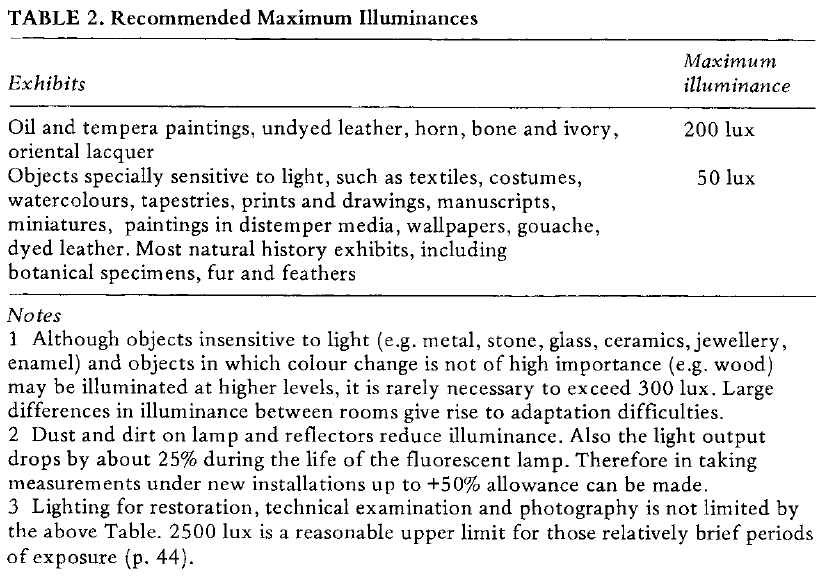
\includegraphics[max width=\textwidth]{figs/LitRev/Thomson.png}
\caption{Table 2 of \citet[p. 23]{thomson_museum_1986}, describing recommended maximum illuminances for 2 groups of objects.}
\label{fig:Thomson}
\end{figure}

Loe et al.'s work concludes with the recommendation that ``preferred artificial lighting conditions for viewing works of art are a painting illuminance approaching 200 lux provided from lamps with good colour rendering characteristics, e.g. a \gls{CIE}~R$_a$ index of \textgreater 85 and a large gamut area''. It is of particular interest to me that Thomson neglected to quote the final part of this recommendation regarding the specific \gls{CIE}~R$_a$ and note regards gamut area.

On the topic of colour rendering, Thomson goes into great depths to explain the topic and the means available for calculating various indices, spending a disproportionate amount of time (compared to what I understand was normal for the time) on the topic of Crawford's `band method' \citep{crawford_colour_1960,crawford_measurement_1959} for colour rendering index calculation amongst other things.

For the most part he neglects to make recommendations for specific target values, only making the rough and unsupported assertion in passing: 

\begin{itquote}{}
Recommendation for good colour rendering. \\
\gls{CIE}~R$_a$ about 90 or better, \\
R\textsubscript{w} (worst R) about 80 or better, \\
and Crawford Class A, B or C
\end{itquote}

No research is referenced to support this recommendation. The inclusion of $R$\textsubscript{w} (the lowest value of $R$\textsubscript{i}) is notable due to its lack of consideration in other documents. 

Still on the topic of colour rendering, of additional note is Thomson's general introduction to the subject, where he frames the conversation in a manner which presents colour rendering as a measure of the colour changes to which the human visual system is unable to adapt to, opposite changes induced by changes in colour temperature to which the human visual system is generally able to adapt easily to. Thomson also provides an accessible, and often quoted summary of the underpinnings of how the \gls{CIE} General Colour Rendering Index operates in principle:

\begin{itquote}{}
Adapt our eyes to the illuminant under test. \\
Look at a set of representative objects under it and accurately memorise their colours.\\
Adapt to the reference illuminant.\\
Look at the same objects under this second illuminant and compare the colours to the colours in our memory.
\end{itquote}

Thomson's comments on the selection of colour temperature are minimal, not referring to any specific \gls{CCT} in his summary of specifications [p. 268]. The only note dealing directly with the specification of colour temperature can be found on page 25, and refers only specifically to the conversation of what colour temperature to select for those environments which for conservation purposes need to be lit at particularly low illuminance levels.

\begin{itquote}{}
The `coolness' \dots of daylight when it has been reduced to 50 lux often gives the impression of gloom, especially when it is highly diffused. No one knows how deeply it has been built into our systems, but ever since our first ancestors sat around fires, and later used oil lamps and candles, the human race has been accustomed to `warm' light in the home after dark. As a result the warm 50 lux from tungsten lamps appears to be brighter, and certainly more cheerful, than 50 lux of diffused daylight. For the same reason warm rather than cool fluorescent lamps should be chosen for 50 lux situations.
\end{itquote}

It is assumed that the views expressed above are grown from empirical observation. They mirror the standpoint of other publications which refer to the work of \citet{kruithof_tubular_1941} and the derived `Kruithof curve' (see Section \ref{sec:CCTmus)}).

The bulk of pages 49-51 concern colour temperature, if one includes the associated discussion of chromatic adaptation and colour constancy, but there is no clear link as to how the author suggests that this theory should be considered in practical application, nor any concrete recommendations for target figures.

A final note in reference to this text goes to the discussion of whether or not to consider the type of lighting for which the artist intended an artwork to be displayed under, or that under which it was originally created. At the risk of quoting half the book I include one final passage which I think particularly pertinent to the area of research to be undertaken in this project, with which I shall conclude my discussion of this publication:

\begin{itquote}{}
I think one would be correct to suppose that artists have always assumed that their creations would be viewed in a variety of situations, not all lit ideally, and have designed their work accordingly. Even the Impressionists and others who made a point of completing their canvasses in the open air did not expect them to be so viewed. When De La Tour painted a candle-lit scene he painted it in such a way that the scene would look candle-lit under any reasonable lighting (for a contrary view see Weale [\citep{weale_truth_1973}]). 

But it could also be said that, however robust the work of art, it will look better in some lighting situations than in others, and so we should bend our efforts to finding the best possible situation. Within the limitations of the museum one cannot but agree, provided there is indeed a consensus of perceptive opinion on what is best, and provided that the damage caused by light is kept under control. 

There is certainly no mathematical treatment whereby we can equate the viewer's gain against the exhibit's loss. However there has been considerable research on the visual process as it is affected by the lighting, and Brommelle [\citep{brommelle_visual_1972}] has carefully related the experimental work to the museum problem.
\end{itquote}

\subsubsection{\gls{CIE} 157:2004 Control of Damage to Museum Objects by Optical Radiation}

This document is a \gls{CIE} technical report, prepared by \gls{CIE} Technical Committee 3-22 of Division 3 ``Interior Environment and Lighting Design''. 

To set the context for the discussion of this \gls{CIE} technical report, first a note to draw attention to the time period during which it was drawn up, since to the future reader there might be some ambiguity as to what the state of the art was at this point. Whilst it is now at the time of writing in 2016 common to find museums using LEDs to display their objects, this was not the case in 2004. It is noted within the text that LEDs are `are not of suitably high colour quality for museum use at present, but have future potential as very low UV power sources.' The increased use of LEDs does not invalidate the contents of this document, but it is worth considering that it was prepared with pretext to address any LED specific issues.

As previously mentioned, this document takes a different approach to the problem of limiting light induced damage in museums, focusing rather on the process of considering the optimal spectral power distributions as opposed to limiting the light levels wholesale. For example, the closest the document comes to making light level recommendations in the manner of `The Museum Environment' \citep{thomson_museum_1986} is in the tabulation of Mlx hour values for predicted noticeable fade. This approach leaves the decision of actual lighting levels to the museum professionals, with the question being `How long do I want this object to last before a noticeable fade has occurred?'

The document is in some ways an endorsement and extension of the approach taken by \citet{harrison_report_1953} (as discussed in Section \ref{sec:DamageIndex}), in which the concept of a damage function was introduced, this being ``an action spectrum that defines the relative spectral responsivity of a receiving material''. The authors of this document note that the work did not originally gain traction due to conservators' scepticism that a single function could represent the vast range of potential museum object (still an intractable problem). Interest was further lessened by the fact that the original work refers only to one very specific type of material - low grade paper. However, the authors of this document argue that the fundamental idea is sound; a damage function (so long as it is genuinely representative to an extent) could be a valuable tool in assessing the appropriateness of different light sources.

The authors then pull reference from further studies focused on a range of other materials, and find low grade paper is actually an outlier in terms of wavelength sensitivity, with many other materials able to be grouped together in type of dependency (if not like sensitivity). Following Cuttle's work \citep{cuttle_lighting_1988} to describe the pre-existing damage functions as simple mathematical relationships, comparison between the variety of newly created damage functions was possible.

Regarding colour temperature, the report states:

\begin{itquote}{}
While the variations of spectral responsivity for individual materials, particularly pigments, remains problematic, the overall tendency for responsivity to increase at shorter wavelengths is reasonably well defined. It has been shown that there is a general effect for the relative damage potential to increase as colour temperature increases [\citet{cuttle_lighting_1988}]
\end{itquote}

This falls short of offering recommendations for colour temperature choice, remaining impartially scientific. However, an included table, reproduced below, makes it clear that the lower the colour temperature, the lower the potential for damage (for a set SPD `type').

\begin{figure}[htbp]
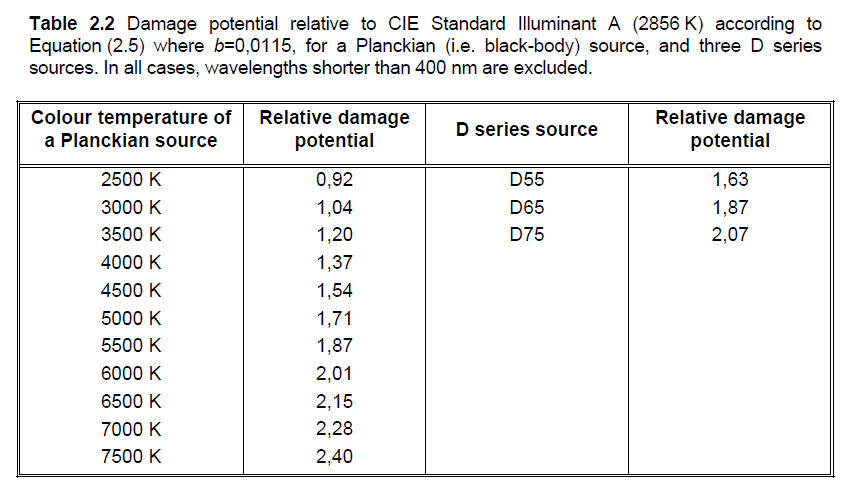
\includegraphics[max width=\textwidth]{figs/LitRev/CIE2004b.png}
\caption{Table 2.2 of \gls{CIE} 157:2004 \citep{cie_cie_2004}}
\label{fig:CIE2004b}
\end{figure}

This section concludes with the introduction of two related topics, again with significance for this project. The first regards the work of \citet{miller_evaluating_1993} in which the concept of \gls{REM} is introduced, the second is of the work by \citet{thornton_high_1975} in which he describes the technique of using `prime colour' light sources.

\gls{REM} in the current context refers to a process of illuminating an object preferentially with illumination of wavelengths which it is known to reflect. The premise of this is: absorbed radiation is visually unimportant, yet conversely the radiation most likely to damage an object. Thus an ideal situation would be to illuminate an object with radiation which it entirely reflects. The immediate limitations of this process are that this process would be object specific and potentially problematic for correct colour rendering. This procedure was suggested to be implemented using fibre optics and filter systems, it would likely be much more approachable with the advent of LED technologies which allow certain spectral flexibility.

A note in the text regards the potential for \gls{REM} to increase the saturation of colours relates that this `raises questions concerning the ethics of modifying the apparent colours of displayed objects.' 

\hl{Thornton/Prime}
\hl{(Colour rendering/critical viewing)}

In the final section of this document (written with the aim to `give recommendations for lighting in museums') very little advice is given in the form of specific figures to aim for, rather a decision appears to have been made that it was preferable to detail the areas that the authors considered worthy of attention, and to lay out the arguments for deliberation. For example, on the topic of \gls{CCT} choice reference is made to the previous discussion which details the deleterious potential of illumination at different colour temperatures, but it is clearly stated that `[w]here the viewing conditions call for moderate or high colour temperature lighting, conservation concerns should not override design objectives for the display.' This seems to be supported by the later statement that `[i]t is thoroughly bad policy to place an object on display, where it inevitably will suffer some damage, and to fail to present it adequately.' It is further noted that low colour temperatures may `judged unsatisfactory' when it is used in combination with natural illumination. 

With marked separation, the previously discussed work of \citet{loe_preferred_1982} is referred to, in the context of providing guidance on a lux value that is `generally sufficient to provide for adequate visibility'.

There is a noteworthy section on the meaningful distinction between illuminance and irradiance: `It needs to be recognised that illuminance is not a reliable alternative measure [for irradiance], as it represents the density of luminous flux, being radiant flux evaluated according to a typical human visual response, defined by the photopic spectral luminous efficiency function V($\lambda$). Not only does illuminance take no account of irradiance outside the visible spectrum, but also radiant flux within the visible spectrum is weighted according to its relative visual effect, which is not related to its damage effect.'

\subsubsection{CGI/Getty Guidelines for Selecting Solid-State Lighting for Museums}

This guidance document \citep{druzik_guidelines_2012}, produced by the Canadian Conservation Institute and The Getty Conservation Institute, provides guidance for museum professionals to select \gls{LED} lighting. As such, the guide includes an introduction to the technological theory of \glspl{LED}, advice on how to consider the requirements of museum lighting, and a practical guide to selecting lighting. It is the only document here considered which discusses solely LED technology.

Compared to the other documents considered here, there is also a focus on the longevity of systems, particularly in respect to potential for colour change, and advice on the type of information that should form a warranty agreement between supplier and end user.

A recurring piece of advice throughout the document is that a lighting specifier should always view lighting in person before making a significant order. The implicit, and sometimes explicit subtext here is twofold; firstly, that the specifications available for lighting are insufficient to describe the visual appearance of lighting, and secondly, that the quality of museum lighting (the ability of lighting to fulfil predetermined requirements) is visually assessable. An extension of this second point would be to consider the visual requirements in museums as being solely or principally defined by a general preference for appearance under lighting.

Following this notion, \gls{CIE}~R$_a$ is referred to as `imperfect' and `misunderstood', and it is suggested that it could be used as a `secondary consideration'. There are several different specific values of \gls{CIE}~R$_a$ recommended at different points within the document.

\begin{itquote}{}
It is generally agreed that a \gls{CRI} above 85 is suitable
\end{itquote}
\begin{itquote}{}
To illuminate areas with a more utilitarian [function] such as machinery, many science exhibits, food services, hallways, educational activities, etc. settle on a color rendering index (\gls{CRI}) above 80. When color matching may be more an attentive activity such as viewing art, ethnography, some natural history collections exhibits, etc. select \glspl{LED} with a \gls{CRI} above 90. However, because \gls{CRI} is an imperfect metric, \gls{CRI} should be considered a target, not a firm criterion.
\end{itquote}
\begin{itquote}{}
There is no international museum standard on what is or is not an ``acceptable'' \gls{CRI}, but the Canadian Conservation Institute (CCI) recommends a minimum of 85. Many museums specify greater than 90.
\end{itquote}

As is perhaps apparent in the quotes above, this document has the feel of friendly advice rather than an official guidance document. As such, it has particular value for this project as a perhaps more revealing account of the advice which actually circulates in the field. For example, one piece of advice which I haven't seen anywhere else in official literature, but which as I understand it is relatively common in general parlance is that provided during the overview on page 23: `Check color rendering on your own skin'. This advice is incongruous with the museum lighting advice which prioritises objectivity and impartiality, as this implicitly suggests looking for a `pleasing' appearance.

The document makes subtle references to the \gls{CQS} \citep{ohno_rationale_2010,baier_is_2012,davis_toward_2005,davis_color_2010} and \gls{GAI} \citep{rea_color_2008}; saying that in response to limitations with \gls{CIE}~R$_a$ `at least two other color metrics have been proposed recently', followed by references which relate to the aforementioned respectively. The document also makes two references specifically to \gls{CIE}~R$_9$ values, firstly as part of the information on the ENERGY STAR program (where it is quoted alongside other lamp specifications) and once in the Appendix (where visual demonstrations of induced colour shifts are provided for the \gls{CQS} and \gls{CIE} test colour samples. Interestingly, a scale for \gls{CIE}~R$_9$ is described, where: `\gls{CIE}~R$_9$ = 0-49 means it renders red hues well. When R9 is 50-74 it is very good. R9 above 75 is considered excellent.' As with many items in this document, no reference as to the source of this information is provided. 

Regards the question of CCT within museum lighting, the guidance offers a Kruithof-ian approach, though without naming it as such, recommending warmer light for lower light levels and colder light for higher light levels. 

\begin{itquote}{}
With low light levels, as in museums, viewers tend to prefer warmer light similar to that of incandescent lamps, e.g. the 2800K of standard incandescent lamps, or the slightly higher 3000K of quartz halogen incandescent lamps. As illumination increases to several thousand lux, preference is for cooler light, 5000K or higher.
\end{itquote}

It is noted than an exception might be made in the situation where artificial lighting is employed to augment natural illumination. This said, elsewhere in the same document the reader is advised to `avoid higher color temperatures for light sensitive materials as these LEDs may have an unacceptably large peak in the ``blue region'' of the spectrum.'

Also poorly referenced is the discussion of the 50 lux recommendation. Research is mentioned but not directly quoted. It is assumed that the research described as `in the 1980s' is the previously discussed research of \citep{loe_preferred_1982}.

The final area of note within this report is that which considers the methods applicable to assessing museum lighting in situ. A survey completed at the Field Museum \citep{myer_demonstration_2010} is quoted in detail, the survey having been completed by museum staff and lighting practitioners as part of a GATEWAY program demonstration at the museum. This survey includes such questions as `The lighting product shows \underline{\hspace{2cm}} of the subject colors accurately' and was completed for a halogen system and an LED system in the same space.

\subsubsection{SLL LG8: Lighting for museums and art galleries}

\citet{cibse_lighting_2015}

% To be written up
% -	Recent doc 2015
% -	Benefits from Practical examples
% -	Lots of big/familiar names
% -	Limited references, no in line sources

% -	Pg 3 CCT warmer light standout?
% -	Pg 4 CRI 90 very good, <80 not suitable
% -	5 colour of backgrounds
% -	9/12 combining daylight and cct
% -	24 `purely advisory' reflect current practice
% -	25 `access has two components, visibility and duration of exposure to light'
% -	27 basing on `good eyesight' might be `discriminatory'
% -	28 distorting intention of artist
% -	33 V&A JNC 50years?
% -	43 trade off
% -	46 blue peak ongoing research
% -	47 essential to conduct side-by-side trials
% -	67 good colour quality = poor efficacy?
% -	Many specific object types

\subsubsection{IES RP-30-96 Museum and Art Gallery Lighting: A Recommended Practice}

\citet{ies_ies_1996}

% -	1996, as of 2016 being updated
% -	Guide for lighting designers

% -	1 `human achievement'
% -	1 Different priorities for different people (kesner)
% -	1 Three rules
% -	2 `Color should not change the look of an artifact' ``overriding – original appearance''
% -	3 CRI ``true color'' >80
% -	3 CCT Determine whether the display takes on a warm or cool appearance
% -	12 30lux required for color
% -	12 avoid bold surrounding colours
% -	13 `killing the patient'
% -	15 lux = exposure(?)
% -	31 Brief history of daylight in galleries
% -	31 adaptation



















\subsection{CCT in museums}
\label{sec:CCTmus}

\Gls{CCT} is often described as an important variable in museum lighting, but definite recommendations, in the rare cases that they are given, are generally based on nostalgia for the appearance of tungsten lighting, questionable research on human preference \citep{kruithof_tubular_1941,fotios_revised_2017} or very rough rules that predict that damage potential will be decreased if \gls{CCT} is minimised \citep{cie_cie_2004}. Whilst some research appears to have found optimal \glspl{CCT} for viewing artwork \citep{nascimento_best_2014,pinto_correlated_2008,scuello_museum_2004,scuello_museum_2004-1, liu_cultural_2013,vidovszky-nemeth_introductory_2016,feltrin_impact_2019} results often have large inter-observer variability, context dependency and it is not uncommon for the headline findings of separate studies to be in contradiction. 

Specifications often refer implicitly or explicitly to the findings of \citet{kruithof_tubular_1941}, who found that at lower levels of illumination, lower \glspl{CCT} were preferred, and that at higher levels of illumination higher \glspl{CCT} were preferred (see Figure \ref{fig:Kruithof}). Whilst this general trend seems to have anecdotal support, it is possible that there may be lighting-technology-based confounds, and recently researchers \citep{vienot_kruithofs_2009} (including a meta-study of multiple other examinations \citep{fotios_revised_2017}) found there to be no substantive support for Kruithof's findings.

% Kruithof is referred to a lot but needs proper discussion somewhere. %DG: I think I do that already above (?)

\begin{figure}[htbp]
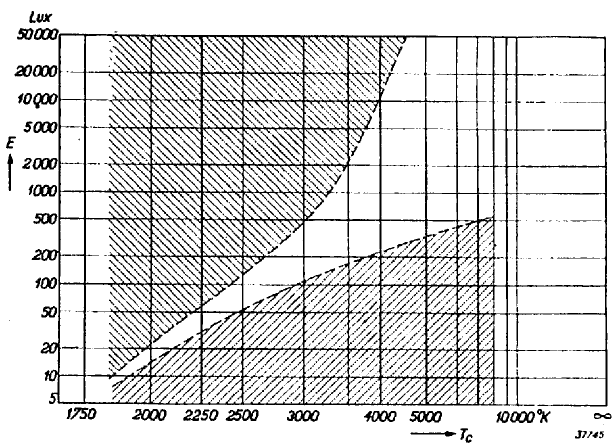
\includegraphics[max width=\textwidth]{figs/LitRev/Kruithof.png}
\caption{The `Kruithof curve' reproduced from \citet{kruithof_tubular_1941}, showing colour constancy against illuminance, and highlighting an area that is considered ``pleasing'' (central white area).}
\label{fig:Kruithof}
\end{figure}

The damage justification seems more substantive; following the application of damage factors as discussed in Section \ref{sec:DamageIndex} the \gls{CIE} published a report showing the varying the \gls{CCT} of museum lighting could have a clear impact on the potential damage undergone by museum objects \citep{cie_cie_2004}. 

\begin{figure}[hbtp]
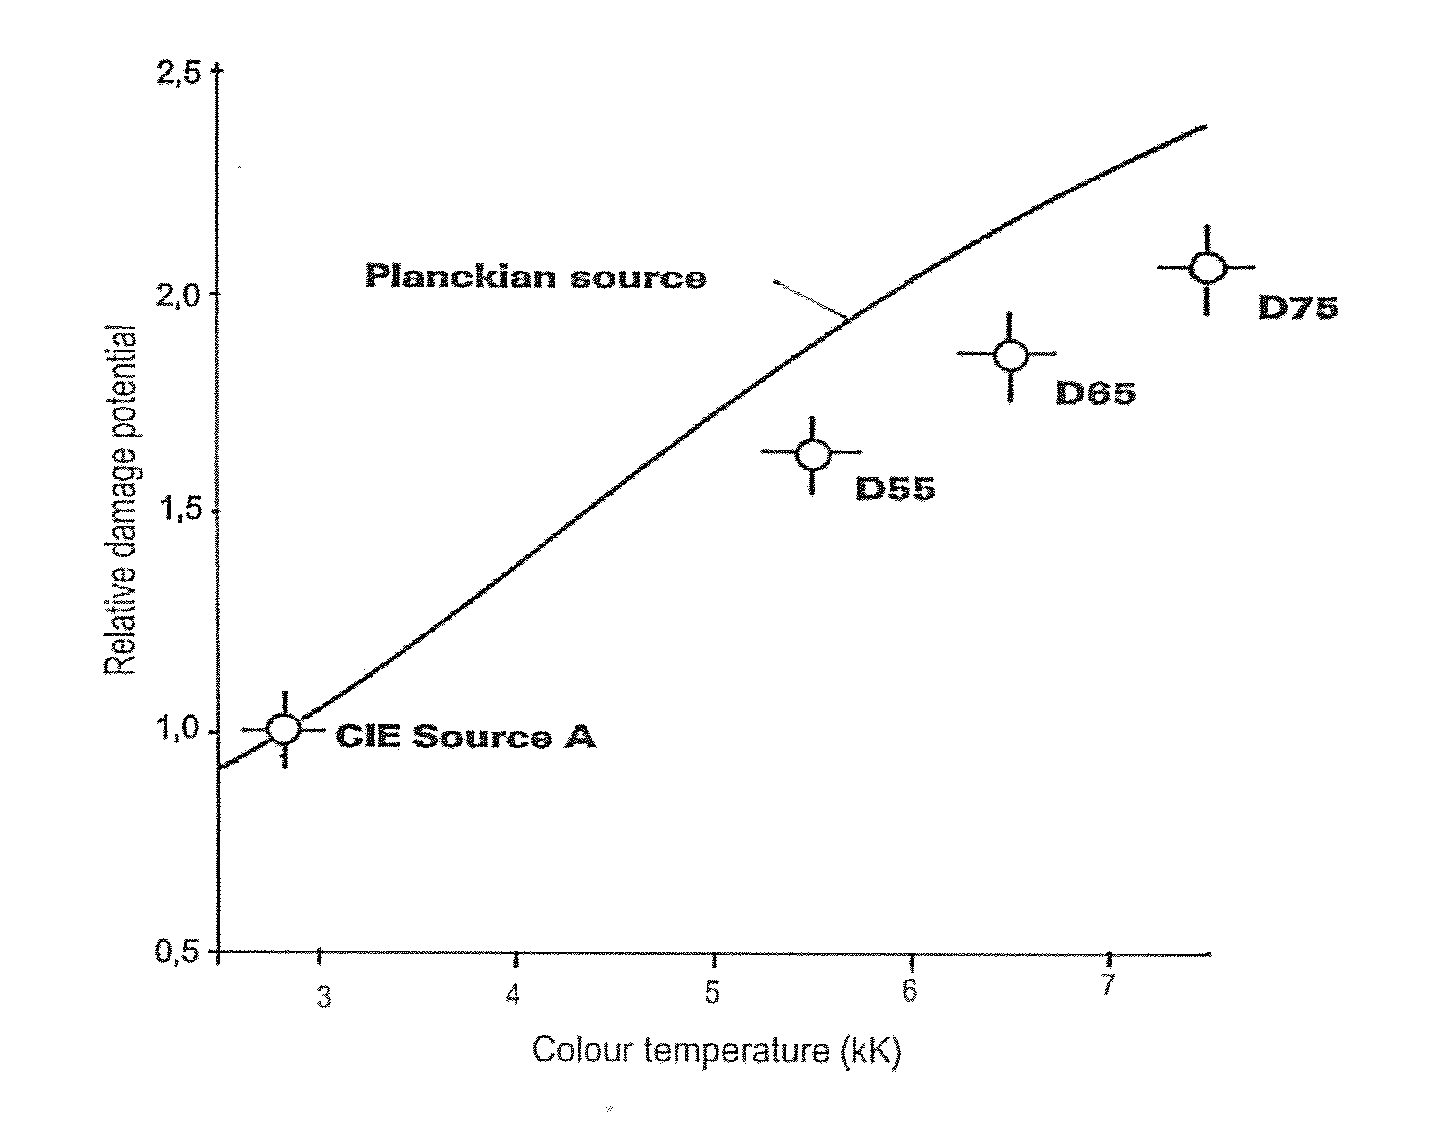
\includegraphics[max width=\textwidth]{figs/LitRev/CIE2004.png} 
\caption{Figure reproduced from \gls{CIE} 157:2004 \citep[p.16]{cie_cie_2004}, showing the relationship between \gls{CCT} and relative damage potential for black body radiator illuminants, \gls{CIE} source A and three \gls{CIE} D-series illuminants.}
\label{fig:CIE2004}
\end{figure}

This line of reasoning relies heavily upon the applicability of damage functions to the specific materials in question. As discussed previously (Section \ref{sec:DamageIndex}) it seems that whilst the generalised damage functions account for some of the individual material damage functions, they do not fully do so. However, tentatively, they do seem to be a relatively good fit for the shared characteristics of different damage functions (at least far more so than V($\lambda$)), and so it seems reasonable to use them where no other broad approximation for a large set of objects exists.

To verify the findings of the \gls{CIE}, extend their findings to \glspl{LED}, and provide code for others to do similar research or even test their own lights/materials, a set of MATLAB functions\footnote{\url{https://github.com/da5nsy/DamageIndex/blob/c7851e27ca1b0915013d8723db04704b49b4085e/CalcDI.m}} have been written (by the author) which calculate \gls{DI} values for arbitrary illuminants. This code has been used to produce Figure \ref{fig:CCTvsDI}, which shows the \glspl{CCT} and \glspl{DI} of the 401 \glspl{SPD} of \citet{houser_review_2013}. A $b$ value of 0.0115 corresponding to `oil paints on canvas' and `water colours on rag paper' (see Table \ref{tab:b}) was used. It can be seen that there is a clear correlation between \gls{CCT} and \gls{DI} with higher \glspl{CCT} being predicted to be relatively more damaging. If a damage function with a lower $b$ value (such as for `low-grade paper' or `textiles') had been used, the relationship between \gls{CCT} and \gls{DI} would be steeper.

%\afterpage{\clearpage}
%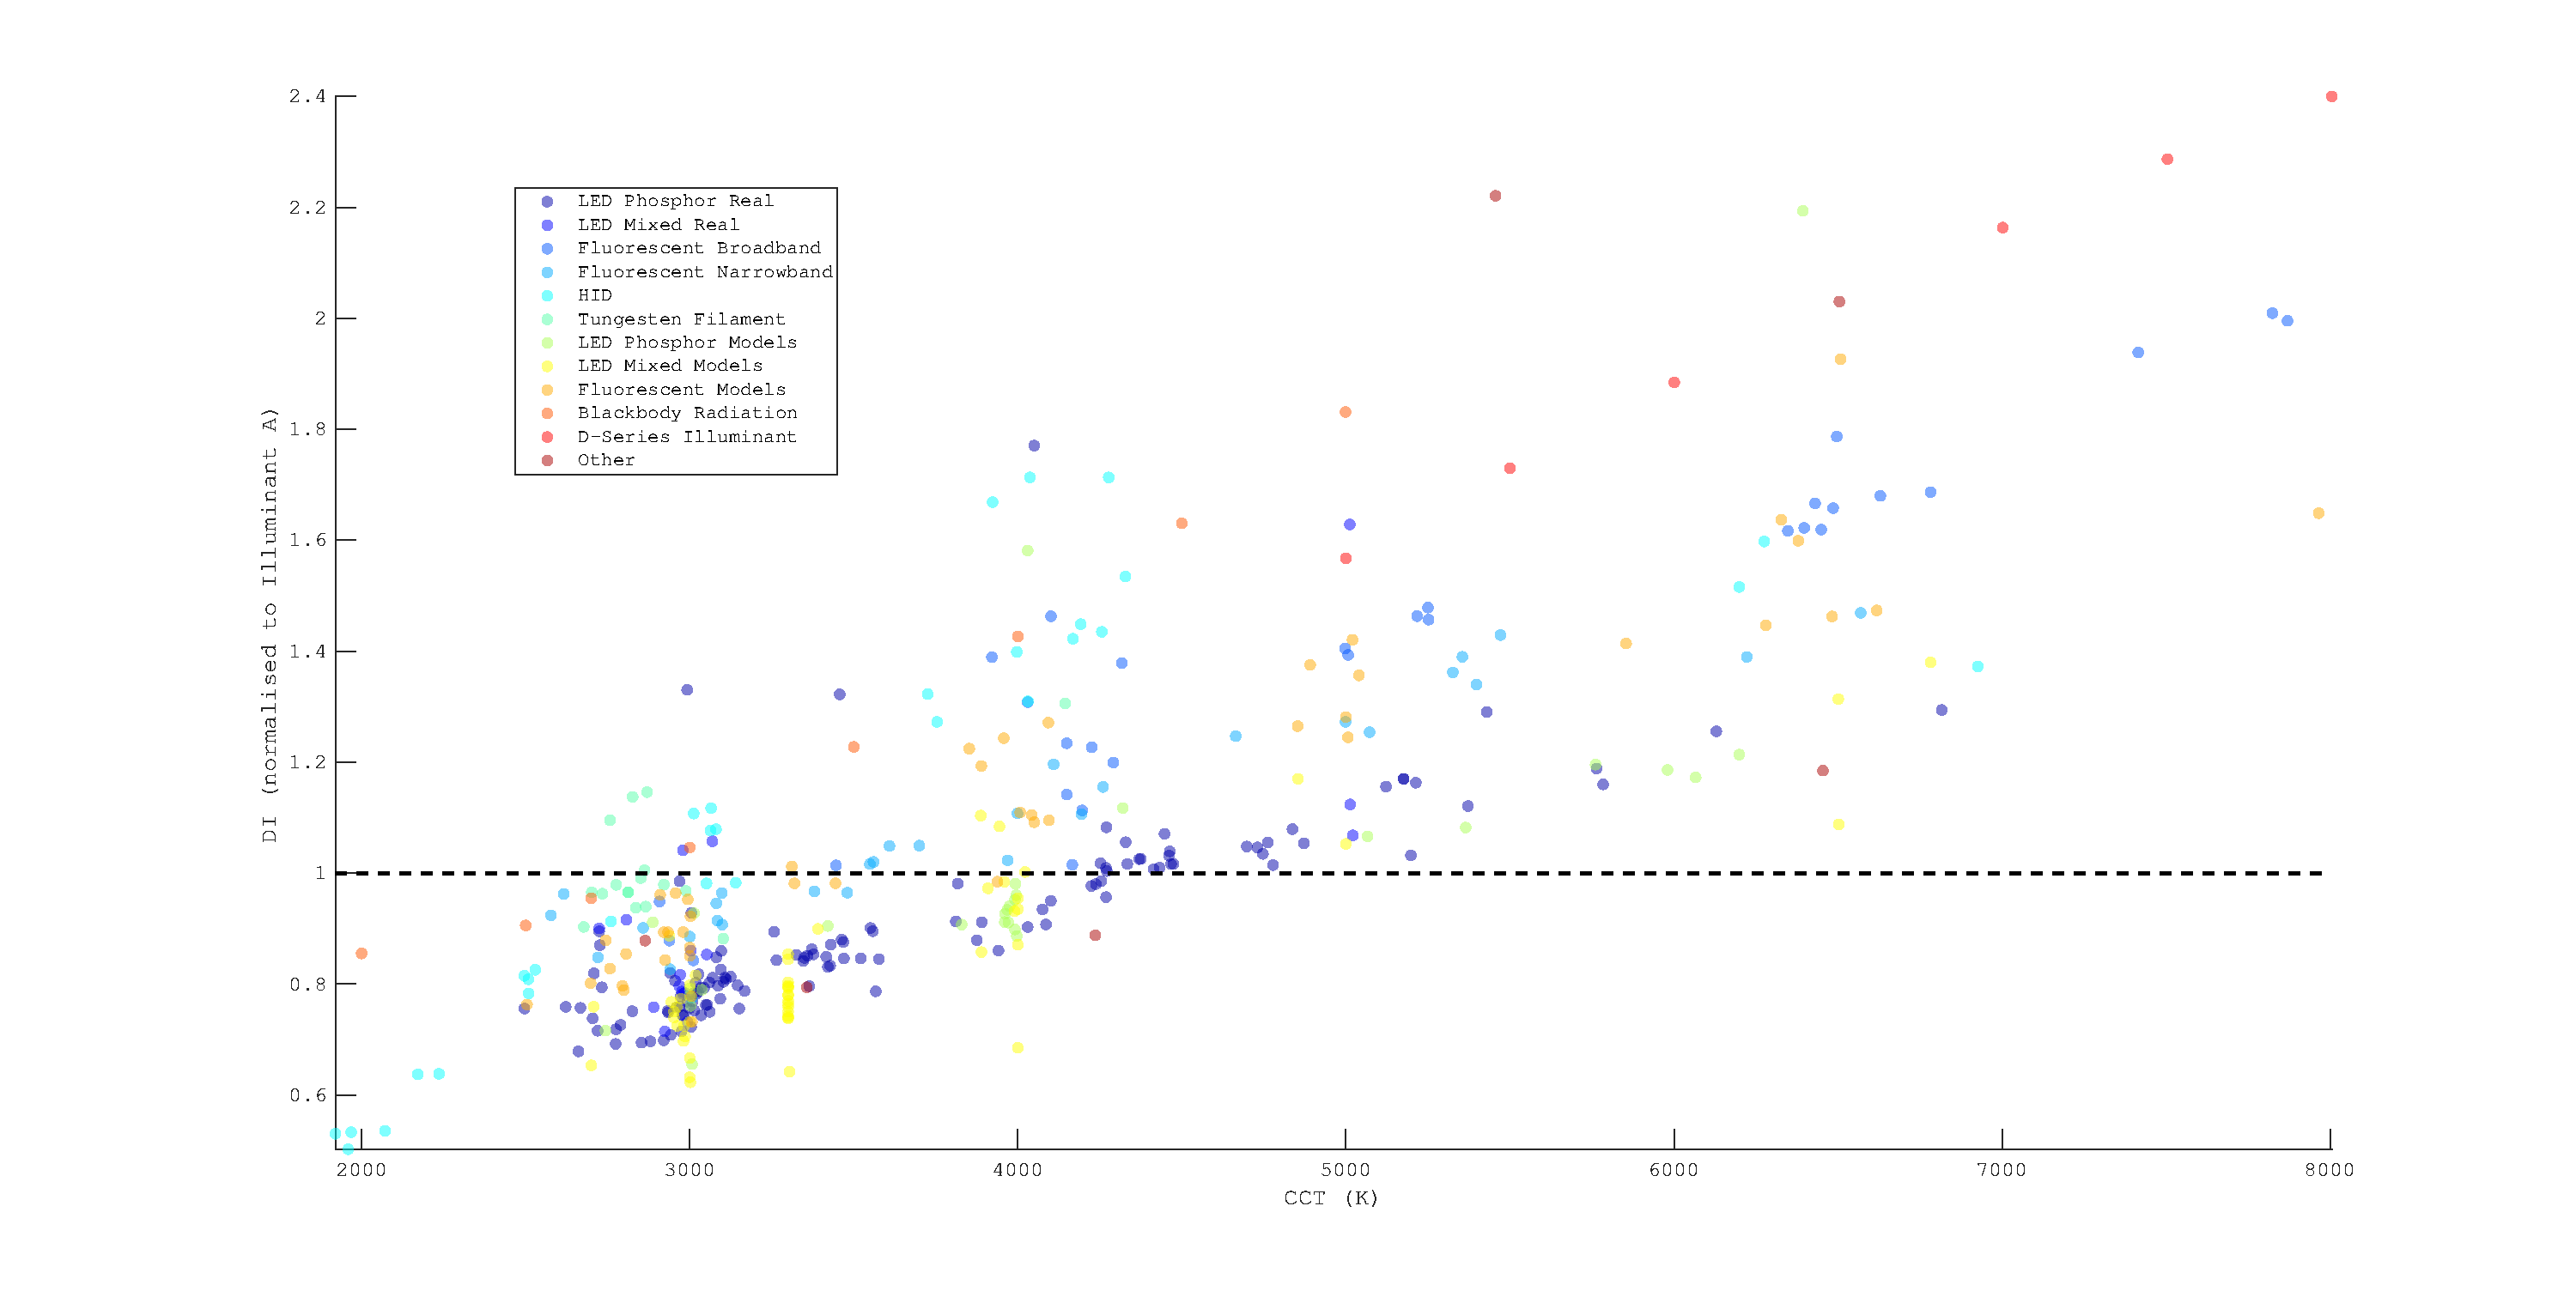
\includepdf[pages=-,rotate=90, offset=75 -75]{figs/LitRev/CCTvsDI.pdf}
% \begin{figure}[t]
%     \caption{The \glspl{CCT} and \glspl{DI} of the \glspl{SPD} used by \citet{houser_review_2013} [provided via personal communication, but now partially available via \gls{PTB} as `spd\_houser'].}
%     \label{fig:CCTvsDI}
% \end{figure} 

\begin{fullpagefigure}
\figpdf[pages=-,rotate=90, offset=-85 -85]{figs/LitRev/CCTvsDI.pdf}
\figpageside{}
\caption{The \glspl{CCT} and \glspl{DI} of the \glspl{SPD} used by \citet{houser_review_2013} [provided via personal communication, but now partially (without category information) available via \gls{PTB} as `spd\_houser'].}
\label{fig:CCTvsDI}
\end{fullpagefigure}

The results of these computations show a clear relationship between \gls{CCT} and \gls{DI}. Considering that this is not currently taken advantage of in museum lighting, it seems as though there is a great potential for reducing damage whilst maintaining visitor visual satisfaction.

%\clearpage
% This is combo with the figpageside thing above currently isn't quite working

%%%% !!!!!!!!!! Check this works before printing

\cleardoublepage %works but seems a bit heavy handed.

\subsection{Colour Rendering Indices in Museums}

%Are fidelity indices suitable for museum use? 
The first chapter of Cuttle's book `Light for Art's Sake: Lighting for Artworks and Museum Displays' \citep{cuttle_light_2007} is titled `A philosophy for the presentation of art'. The choice of title here is apt but may surprise some readers, sounding more whimsical than might be expected of a serious subject attended by scientists and engineers. The reason it is so apt is because lighting is unavoidably a creative intervention\footnote{Credit for this phrase to Katherine Curran} which is to say that there is no lighting which is truly impartial, and no lighting which is truly `correct' in the sense of being unequivocally superior to another. All lighting decisions require choices to be made, and whilst these choices can be wrapped up to appear as an optimisation problem where proximity to a particular solution is the goal, the problem always rests on the bedrock of a philosophy based decision.

In the above mentioned chapter Cuttle lays out a total of seven distinct philosophical propositions, which he poses for consideration as approaches to museum lighting, some contradictory and some with the potential to overlap:

\begin{enumerate}
\item To make the artwork appear as it would have appeared to the artist at the time of its creation
\item To ensure that no damage due to light exposure will occur
\item To achieve the best possible appearance of the artwork
\item To provide optimum conditions for viewing art
\item To impart a sense of having seen `the real thing'
\item To assist viewers to understand the displayed objects and their reason for being there
\item For the lighting designer to establish a distinct and recognisable style
\end{enumerate}

These propositions refer to museum lighting holistically, considering all aspects of museum lighting, but can be readily focused on the problem of colour appearance specifically. Before we narrow our gaze however, it is worth briefly considering a wide view of lighting attributes which may aid in the realisation of `good quality' museum lighting. Consider Rosenfeld's list of the five `controllable qualities' in museum lighting; `intensity, movement [temporal artefacts], angle [modelling, avoiding glare and reflections], distribution [ambient lighting vs. spot lighting], color' \citep{rosenfeld_agony_2013}.

Whilst Cuttle's propositions make for interesting discussions and enjoyable extended pondering, they are of limited assistance in the practical task of actually specifying lighting. Thankfully, a range of tools exist for the examination of the colour rendering properties of a light source, in the form of indices which aim to numerically describe an illumination's effect on colour appearance of the objects of which it is tasked with illuminating.

Traditionally, colour rendering indices aim to offer a standardised method for calculating the colour differences induced by the substitution of a reference illuminant with a specific test source, and for comparing the relative merit of different test light sources on their ability to induce minimum change. In modern parlance this type of index should be referred to as a colour fidelity index, that is - one which is conceptually concerned with colorimetric reproduction. The term `colour rendering' has come to encompass much more than just fidelity.

Diametrically opposed in some ways to fidelity are the indices which aim to quantify `preference'. In the simplest case, a preference index will aim to provide a value that is predictive of how an observer would rate a light source against other light sources. 

Within and between these two groups there exist a range of different indices with subtly different aims and mechanisms for achieving these aims. For thorough overviews see \citet{guo_review_2004} and \citet{houser_review_2013}.

In practice, both of these philosophical approaches are mandated in current lighting guidance. For the most part, advice for lighting specification on the subject of colour rendering can be simplified to read `use lamps of above \gls{CRI} 80 (referring tacitly to \gls{CIE}~R$_a$) but always test them visually before you buy in bulk'. Whilst this may at first seem like sensible advice, upon further inspection it actually represents a serious contradiction, unless considered with heavy caveats. The problem rests in the fact that \gls{CIE}~R$_a$ is a fidelity index, whereas any visual inspection is likely to be performed by observing the appearance of an object under the test illumination without a reference. Fidelity aims to describe accuracy of reproduction, but this is a quality which is arguably not testable by visual inspection. This contradiction seems to perpetuate unnoticed in museum practice, with lighting specifiers often abstractly declaring to target a faithful/accurate/honest/impartial representation of objects, but practically choosing light sources based on visual inspection where preference is the only criteria. There is of course a range of approaches, ranging from pure reliance on indices to almost entire reliance on visual testing.

In conclusion, no one metric exists that would satisfy the divergent aims and philosophies of museum lighting. Several distinct types of colour rendering index exist, but the existing range fall into the broad categories of `fidelity' or `preference', with the latter being particularly poorly definable due to its variability in different environments, with different user functional requirements and different intrinsic preferences between different observers. Progress could be made by breaking these broad categories into smaller more manageable specific objectives.

%weale_truth_1973

%vienot birds
% vienot_leds_2011

%bespoke colour rendering indices, sistine chapel
% schanda_new_2014

%correcting for hunt effect
% wei_consideration_2018



%%%% BONUS AREA %%%%%%%%%%


%\subsection{LEDs in museums}

%%%%%%%%%%%%%%%

%Theoretically, there exists a division between recommendations which deal with visual appearance and those which deal with physical degradation; the first group supported by the science of human vision, and the second supported by material sciences and chemistry. Whilst it is important to be aware of this distinction, it is normally not possible to consider them entirely separately in practice, as many variables will affect both.

%%%%%%%%%%%


%Extending the question of visibility is the subject of appearance. It is a general expectation that museums represent objects in a truthful and impartial manner, and it seems sensible that decisions concerning the appearance of items in museums should be made with this in mind. Alongside this, many museums treasure items where part of their value is aesthetic2, and it follows therefore that a technique which aids in the beautification of an object might be of interest, and this might be particularly of interest if the object is known to have deteriorated since the time of production.

%%%%%%%%%%%

% \subsection{Lighting at The British Museum}

% Lighting at the British Museum has developed in a somewhat organic manner, from the early days of the museum before the introduction of artificial lighting. This leaves the museum with more than sufficient daylight in most spaces during daylight hours, where the increased modern knowledge regarding the deleterious effect of lighting now means that conservators must find ways in which to limit this natural resource so that objects are not unduly exposed. 

% The gallery lighting is replaced when a gallery is refurbished, and the latest technology is installed when a new gallery is created, where viable in terms of suitability and considering financial limitations. Other than this, lighting technologies tend to not be updated other than to replace individual lamps. This coupled with the grand scope of the museum, which means that it is rare for multiple galleries to be refurbished simultaneously, has led to a vast array of lighting designs and technologies. It in fact appears to represent a rather special example of `museum lighting through the ages', with daylight, tungsten, fluorescent and metal halide lamps all seemingly represented, as well as various illumination geometries reminiscent of the times of their fitting. It should be noted that these assertions are made following empirical observation with spectrophotometers and not from conversations with museum staff, see section 3.3 Collection of \gls{SPD} Data at British Museum.

% There also seems to be a great range of lighting quality within the British Museum, with some spaces feeling bright and others comparatively gloomy. There is a range of colour temperatures and chromaticities of light at the museum, as shown in Figure 1.

% Multiple methods are currently employed to limit the exposure of objects in the museum. \Gls{UV} absorbing film or glazing which incorporates \gls{UV} reduction is used throughout the museum and in certain galleries there are automatic blinds which limit the intrusion of direct sunlight at specific times of the day and year. For particularly sensitive objects, rooms are lit artificially at very low levels, and some objects are selectively lit in order to further limit their accumulative exposure.

% 

\section{Mathematical Methods}

A small number of mathematical methods which may not be familiar to the reader are used within this thesis. They are outlined below.

\subsection{K-means clustering}
\subsection{Principal Component Analysis}



%\chapter{Large Sphere}
\label{chap:LargeSphere}


%\chapter{Small Sphere Experiment}
\label{chap:SmallSphere}

\textit{The work presented here has been presented as an invited oral presentation by Lindsay MacDonald at AIC 2017 \citep{macdonald_melanopsin_2017}\footnote{The proceedings are not currently available online, though a note at \url{https://aic-color.org/page-18077} suggests that they will soon be available.}.}


\section{Summary}

\hl{insert summary.}

This study was approved by the \gls{UCL} Ethics committee (Project ID Number: 9357/003), application attached as Appendix \ref{app:ethics3}. Code and data are provided: \url{https://github.com/da5nsy/Small-Sphere}.

\section{Introduction}

% why this experiment? Response to issues in large sphere
% - luminance
% - too many variables
% research question

This experiment was performed to develop upon the Large Sphere experiment (Chapter \ref{chap:LargeSphere}) by narrowing down the number of variables and more directly exploring the question of whether melanopsin plays a role in colour constancy. This was achieved using a similar experimental set-up to the previous experiment, with several key alterations:

\begin{enumerate}
    \item Instead of 16 surround conditions, only two were included.
    \begin{enumerate}
        \item These two conditions were generated through use of narrowband LEDs rather than filtered white light, designed to be perceptual metamers for each observer, but with maximally different levels of melanopic activation.
    \end{enumerate}
    \item Instead of 16 lightness conditions, only 5 were included.
    \item The sphere used was smaller, and the inner surface was painted with a higher reflectance paint, with the hope of increasing the level of adapting radiation.
    \item Three observers were tested (the author and two colleagues of a similar age), with repeats of each condition.
\end{enumerate}

Further details on all of the above amendments will be included in the following sections. 

The null hypothesis that this experiment aims to test is that melanopsin activation does not alter an observers perceptual white point.

\section{Materials and Methods}

\subsection{Hardware}

The sphere used in this experiment was 400mm in diameter, with ports of similar functions to those in the Large Sphere. On one side there is a padded port for an observer's face. Mirroring this is a small aperture through which an LCD screen is visible. At the top of the sphere was a port through which adapting illumination was provided. An additional port, on the observer's side of the base, was added such that the illumination provided to the sphere could be unobtrusively monitored throughout experiments.

\begin{figure}[htbp]
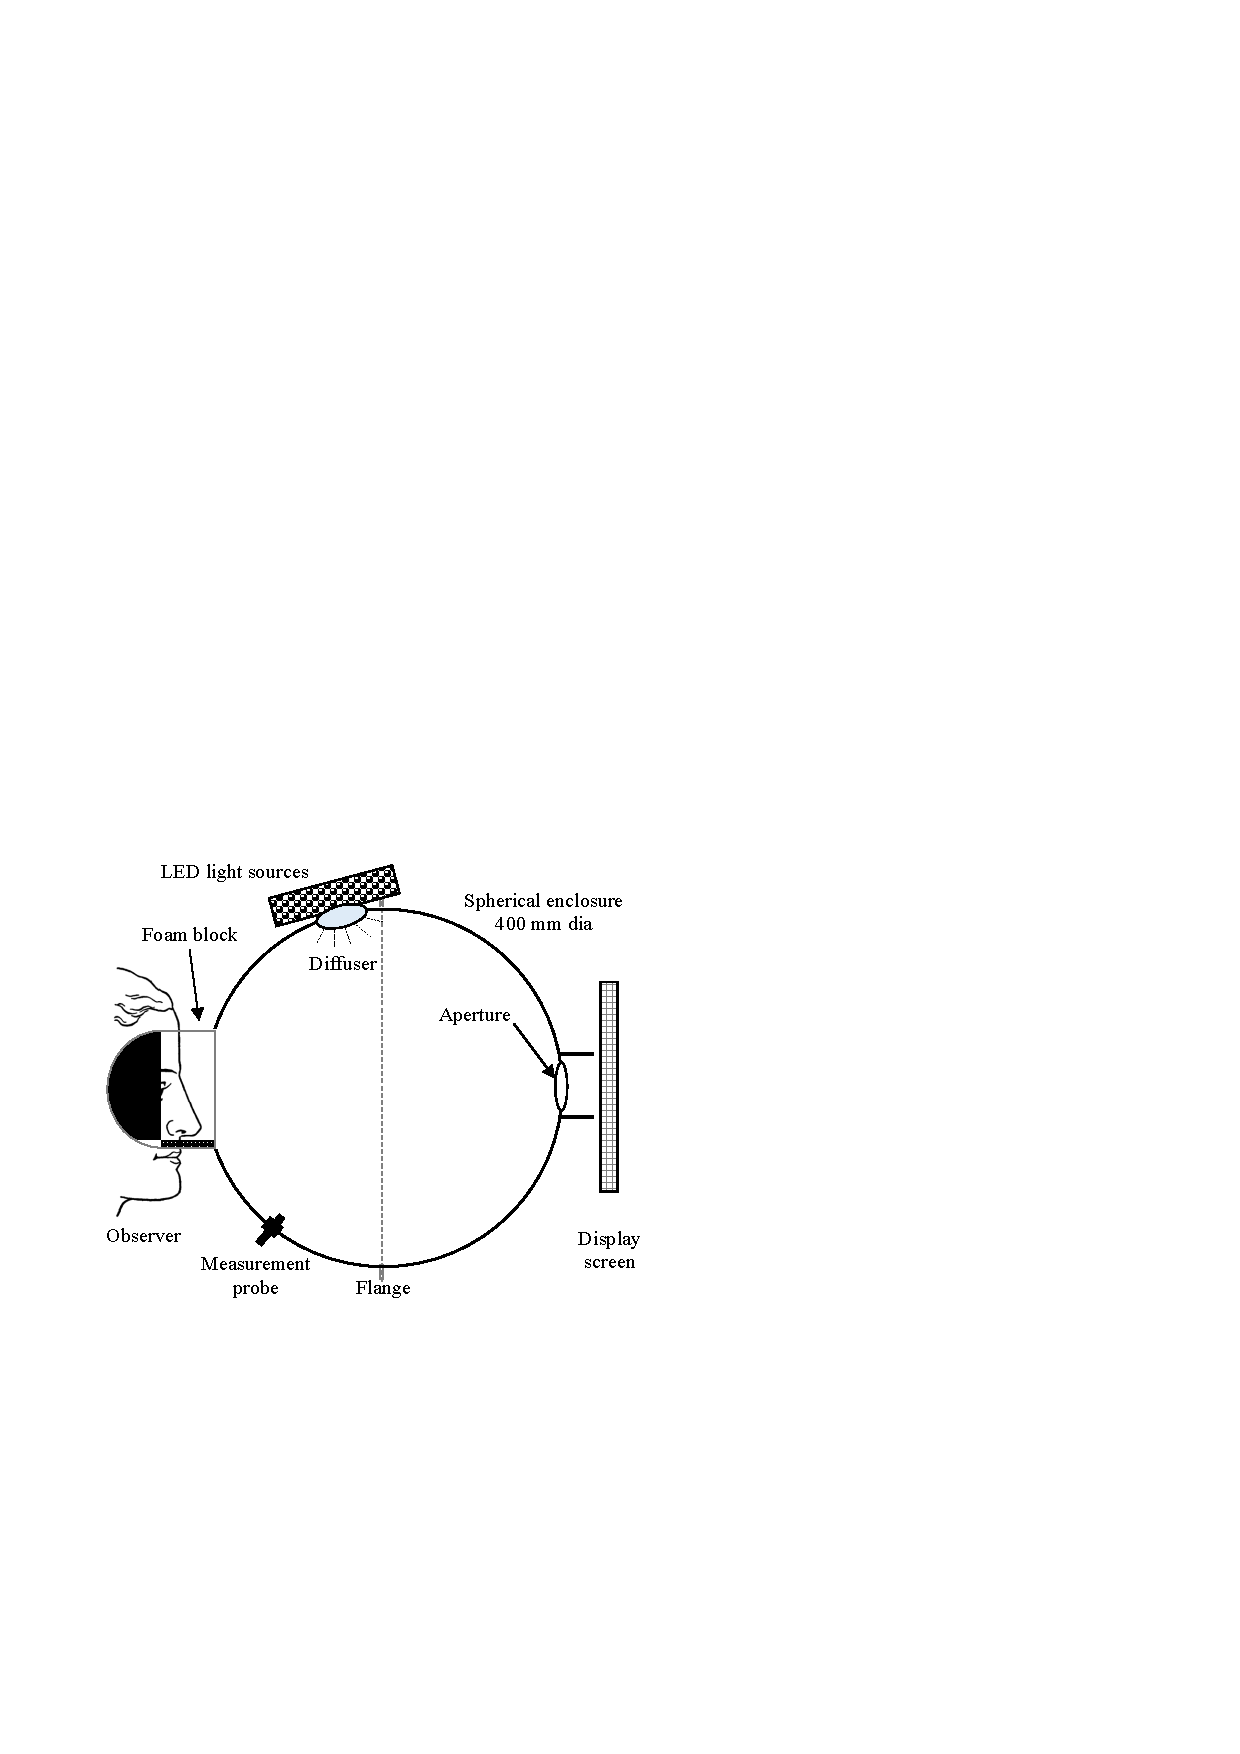
\includegraphics[max width=\textwidth,center]{figs/SmallSphere/diagram.pdf}
\caption{The small sphere set up, reproduced from \citet{macdonald_melanopsin_2017}, courtesy of Lindsay MacDonald.}
\label{fig:diagram}
\end{figure}

\subsection{The sphere}

% how big was the fixation?

% diagram 
% photo

The sphere used in this experiment was smaller than that in the previous experiments (hence the experiment short-hand names) and this served several purposes. The illumination in the Large Sphere had been rather low, partly such that rod interactions would be made visible, and partly due to practical limitations. The grey paint on the interior of the Large Sphere was chosen such to limit specular reflections, but it meant that overall illumination levels were very low. In the small sphere, it was hoped that by reducing the size of the sphere it would be possible to increase the level of illumination, as it would be spread across a smaller surface. Additionally, of practical concern, it was easier to find experimental space for a smaller sphere.

Several paints were trialled for use in the small sphere. The required conditions were that they were available as a spray, and provided as `matt white'. Sample patches were sprayed upon a piece of opaque perspex to assess finish and spectral reflectance. It was seen as beneficial if: the finish had a very fine grain and as little gloss to it as possible, the surface reflectance was high and the \gls{SRF} was as uniform across the spectrum as possible. It was also considered a requisite requirement that any paint should not include any fluorescent whitening agents (such as can be seen in the `white paper' shown in Figure \ref{fig:spray}).

Measurements of the \glspl{SRF} of the 8 tested spray-paints, and further details of the spray-paints themselves, can be seen in Figure \ref{fig:spray}. Measurements were made with a \gls{PR650}, illuminated at 45$^{\circ}$ and measured at 90$^{\circ}$. It can be seen that Montana Gold Sh. White Cream and Pebble, along with MTN 94 RV-198 are either too low in reflectance, or not spectrally uniform enough. The two with the most desirable finishes were the Flame Blue and MTN Water Based paints. The MTN Water Based paint was chosen due to its particularly fine-grain finish.

%The sharp drop off in the \glspl{SRF} suggest that most of the tested paints were titanium-based (based on comparisons to measurements made by \citet{cosentino_fors_2014})\footnote{It is unfortunate in some ways that the \glspl{SRF} drop so rapidly around 400nm, as this means that the one of the chosen LEDs with a peak output of around 400nm will lose a great deal of its power in the interaction with the paint. On the other hand - this decreases the risk to the observer of being exposed to exessive amounts of short wavelength radiation.}.  

\begin{figure}[htbp]
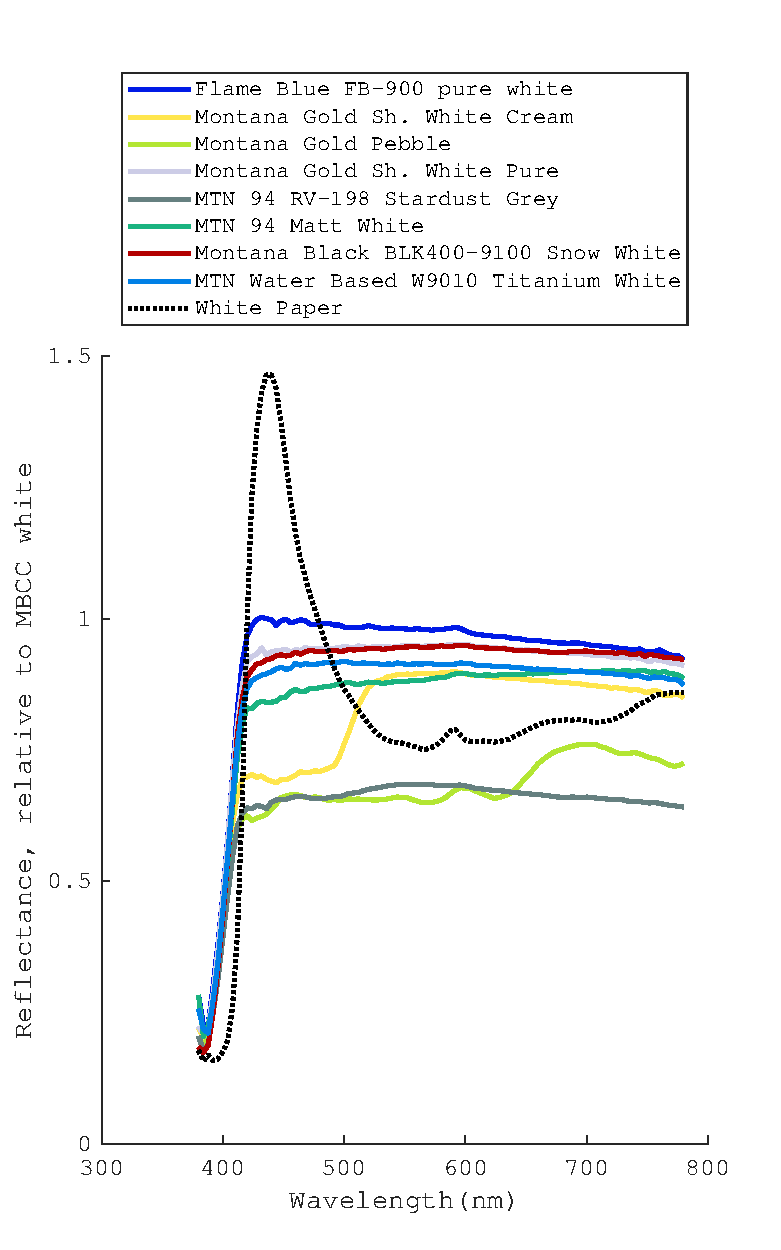
\includegraphics[max width=0.9\textwidth,center]{figs/SmallSphere/VisualiseSPDs_result.pdf}
\caption{The \glspl{SRF} of the 8 tested paints (relative to the white patch of a MacBeth Colour Checker card) with an additional measurement of a piece of white office paper to demonstrate how a fluorescent additive might appear. Data available: \url{https://github.com/da5nsy/Small-Sphere/tree/master/Hardware\%20Specs/WhiteSprayPaints}}
\label{fig:spray}
\end{figure}


\subsection{The screen}

The screen was offset by roughly 150mm through a short black paper tube in order to limit the interference (either way) between the screen emission and the sphere illumination. 

%Primaries
%Gamut

% Out of gamut LEDs?

\subsubsection{Characterisation}

Following issues potentially stemming from uncontrolled variations of display output during the Large Sphere experiment, two separate characterisation procedures were performed, after every set of observations (in addition to the monitoring of illumination inside the sphere).

The primary characterisation routine was as standard - a spectral measurement of the display primaries followed by a ramping through intensity for each display channel from zero output to maximum output\footnote{Controlled by the script available at \url{https://github.com/da5nsy/Small-Sphere/blob/5c6af38c5036a4c0a328a9854427ae8e851e84fd/Hardware\%20Specs/PR650\%20Screen\%20Measurements/PR650displaycharacterisation_DG.m}}. This was only measured for the small portion of the screen which would be seen during experiments.

The secondary characterisation procedure attempted to detect any issues which may arise due to the specific specification method used within the experiment. The MATLAB experimental script was modified to provide a `characterisation mode', with a greatly reduced number of trials (15 total). This mode otherwise performed in exactly the same way that the main experimental script normally would, and the observer was replaced by the \gls{PR650}, and no effort was made to select neutral points, with a measurement being made of each presentation directly. In this way, a random selection of points were recorded, and through comparison with the recorded `responses', it could be seen whether there was any discrepancy between what we thought was being displayed on the screen and what was actually being displayed on the screen.
% demo?

\subsection{The LED rig}

The lighting in this experiment was designed such that two lighting conditions could be defined for each observer which were perceptual metamers (in the periphery, at high temporal frequencies), but which differed in melanopic activation.

Four types of LED, to operate as two pairs, were chosen to maximise melanopic contrast between the pairs. An additional limitation was that no LED with a peak wavelength shorter than 400nm was to be used (due to safety concerns).

50 LEDs, mounted in a breadboard, were controlled by an Arduini Uno. %photo?

\begin{itemize}
    \item 20: Bivar UV5TZ-400-15 (henceforth `UV')
    \item 10: Cree C503B-BCS-CV0Z0461 (henceforth `blue')
    \item 10: Cree C503B-AAS-CA0C0251-015 (henceforth `amber')
    \item 10: Cree C503B-RAS-CY0B0AA2 (henceforth `red')
\end{itemize}

%UNOPENED 
%810-6705 C503D-WAN-CCbEb151
%810-6636 C503B-AAN-CY0B0251
%810-0492 C503B-BCN-CV0Z0461

\begin{figure}[htbp]
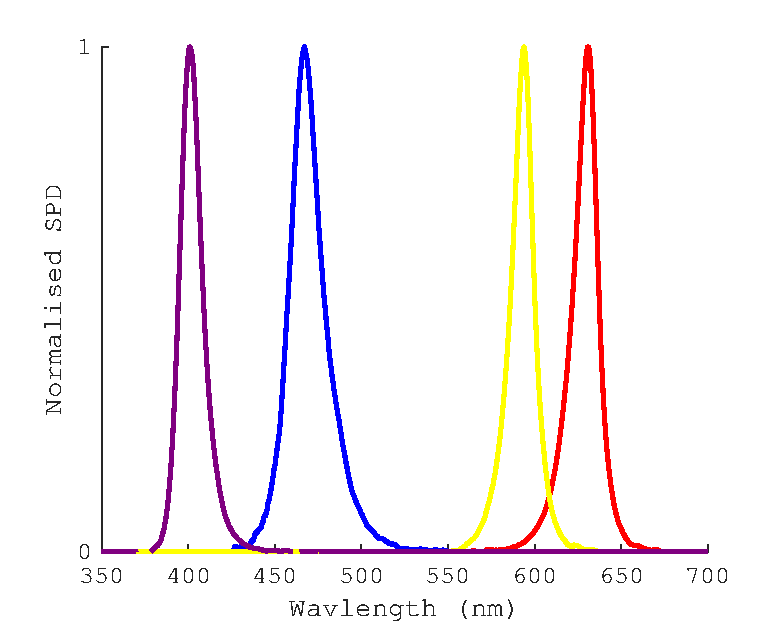
\includegraphics[max width=\textwidth,center]{figs/SmallSphere/LED_SPDs.pdf}
\caption{The normalised \glspl{SPD} of the Small Sphere \glspl{LED}, with lines connecting the pairs which were activated simultaneously.}
\label{fig:LED_SPDs}
\end{figure}

The arduino script set the \glspl{LED}, via pulse width modulation, to the output levels decided in the perceptual nulling segment of the experiment. The two modes had either the combination of UV and amber, or blue and red, allowing for the chromaticities falling upon the lines shown in Figure \ref{fig:LED_SPDs}. The combinations UV and blue, or amber and red, were never used.

\begin{figure}[htbp]
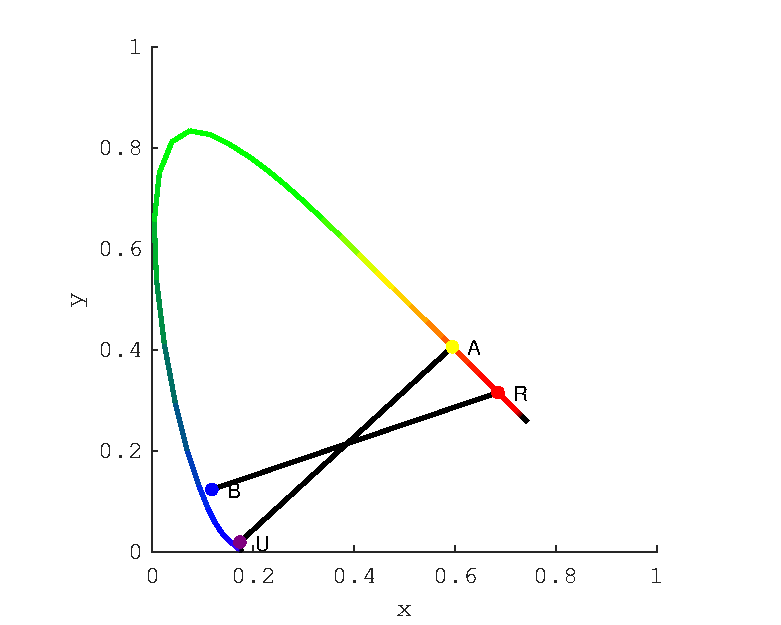
\includegraphics[max width=\textwidth,center]{figs/SmallSphere/LED_cross.pdf}
\caption{The chromaticities of the Small Sphere \glspl{LED} in CIE 1931 space. Thus from each pair, illumination with chromaticity values extending along each line was generatable. Even if there were differences in the spectral sensitivities of the observers (compared to the CIE 1931 observer), with these narrow-band primaries there should theoretically always be a point at which the two lines cross.}
\label{fig:LED_cross}
\end{figure}

This breadboard was mounted stably atop the sphere with a perspex diffusion sheet between it and the opening into the sphere. Black card was used to mask stray light, mainly to address the specific concern that light may fall onto the LCD display.

%LM: photo of the construction of the lighting rig (close up)

Throughout the experiments the illumination inside the sphere was measured with an Ocean Optics USB 2000+ through a optical fiber probe mounted to the base of the sphere and directed at a point on the roof of the sphere, opposite the observer. It was expected that the output of the \glspl{LED} may change slightly over time. %fig x?

\subsubsection{Light safety}
Since illumination of wavelengths shorter than 400nm would be present, it was deemed appropriate to take extra precautions to ensure the safety of participants. 
The implementation of the `BS EN ISO 15004-2:2007 Ophthalmic instruments - Fundamental requirements and test methods - Part 2: Light hazard protection' \citep{iso/tc_172/sc_7_ophthalmic_optics_and_instruments_bs_2007} provided in the Silent Substitution toolbox\footnote{\url{https://github.com/spitschan/SilentSubstitutionToolbox}} created by \citet{spitschan_selective_2015} was used to evaluate the safety of the experimental set-up, and under the default assumptions for pupil size, and with the maximum output from the LEDs, the stimulus was found to be considerably below the limits for type 1 continuous wave instruments. See Appendix \ref{app:ethics3} for further details.

% safety
% The controllers 
% The code
% Characterisation / ongoing measurement

\subsection{Observer task}

\subsubsection{Perceptual Nulling}

The basic logic of this experiment is as follows: under the null hypothesis two adapting fields of identical appearance should cause an observer to be adapted in exactly the same way. In order to design two adapting field illuminants which appear identical (perceptual metamers) we can either make predictions based upon standard observers (with parameters set to match our real observers regards age and pupil dilation etc.) or we can employ a process whereby individual observers make minor alterations to two conditions, that are designed such that they could be metamers, until they appear identical. We have opted to use colorimetry as a starting point to choose primaries (Figure \ref{fig:LED_cross}), and then allow observers to fine-tune this matching.

We run the risk of falling into circularity here: we ask observers to set two fields such that they appear identical, and then (in a roundabout way) we ask them whether there is any visual difference between them. If melanopsin does have a direct impact upon visual perception we are at risk of accounting for this at this stage. In an attempt to avoid this problem, we perform the perceptual nulling under conditions which we predict should not allow for \gls{ipRGC} involvement, or should minimise such. It seems to be the case that \glspl{ipRGC} do not react strongly over very short timescales ($<$0.5hz \citep{spitschan_human_2017-1}), with cones being much more active in this temporal window, so we chose to alternate rapidly between the two conditions and ask observers to make alterations until there is a minimal visible flicker.

Observers were instructed to fixate upon a small fixation point displayed at the centre of the otherwise dark display. They placed their hands upon three dials which could be independently varied to change the peripheral adapting illumination inside the sphere.

Two modes were presented to observers, one where the two conditions were alternated at 30hz for 1 second, followed by a 10 second break, and one where the conditions were alternated at 4hz for 500ms, followed by a 1 second break. 

During the first condition the observer was requested only to alter the setting of the first dial, which would change the overall level of the red/blue combination (whilst the uv/amber combination remained at the same level). This was referred to as brightness matching.

During the second condition the observer was requested only to alter the settings of the second and third dials. The second dial would alter the relative contributions of red/blue to the first condition. The third dial would alter the relative contributions of uv/amber to the second condition. These options can be thought of as traversing the straight lines in Figure \ref{fig:LED_cross}. This was referred to as colour matching.

%LM: photo of observer looking into sphere

The observer was allowed to switch back and forth between these two modes until they were happy with the match. Once an observer had indicated a match, the LED drive values were recorded and these were used for the observer in future sessions.

Observers found this task rather arduous, predominantly due to the inherent difficulty in making colour matches in the periphery. An additional difficulty was that since eye movements were not strictly controlled, if an observer were briefly to look away from the fixation they would be able to see the adapting field with their foveal vision. This was problematic since in most cases the peripheral matches induced strong contrast for foveal perception. Though it was unintentional, this seems to be a particularly effective way of generating the perception of a Maxwell spot \citep{isobe_functional_1955}. Further to this, the authors' experience was that the visible periphery could be further divided, by eccentricity, into two or possibly three areas where a match in one area would not provide a match in both areas.

Despite these difficulties, observers generally found settings which for them resulted in a metameric match (where they could no longer perceive flicker, or perceived minimal flicker). One observer who initially agreed to be part of the study withdrew at this stage, partly due to a difficulty completing this task, but mainly due to a claustrophobic reaction. Another potential observer withdrew at this stage, since he was unable to make a match using this set of primaries, which we tentatively attribute to incipient cataracts.

This method has since been further developed by \citet{allen_form_2019} who used a 2AFC task instead of a method of manual adjustment to pinpoint areas of perceptual metamerism.

% Observers were...
% Initial metamer setting
\subsubsection{Achromatic selections}

3 observers took part in the main experiment (the author (DG), HC, and LW). 

The task was identical to that performed in the Large Sphere experiment; using two sliders (controlling the yellow/blue component and the red/green component) to set the foveal stimulus to appear achromatic. As previously noted, instead of 10 runs of L* 85 descending in 5* increments to L* 10, there were 30 runs of a pseudo-randomly permuted (each run) set of stimuli specified such that there was one at every 10 L* interval between 30 L* and 70 L*. The range was reduced so as to minimise the impact of gamut-boundary issues. The L* interval was increased to allow for a greater number of repetitions of specific values within a similar time frame. The order was pseudo-randomly permuted to avoid any trend based effects.

Two observers (HC and LW) performed 4 complete runs each, 2 under each condition. The author completed 2 runs, one under each condition. Each observer only completed one run per day. There was a gap of roughly three months between the initial runs of HC and LW and the repeat runs.

\subsubsection{Data Analysis}

Following calibration, for each observer under each condition, the means and standard deviation were computed for each dimension of CIELAB. The inter-condition mean vectors were calculated.

The data were submitted to a two-sample two-dimensional Kolmogorov-Smirnov test\footnote{Using the function available from \url{https://uk.mathworks.com/matlabcentral/fileexchange/38617-kstest_2s_2d-x1-x2-alpha}.} to compare the two distinct conditions for each observer (including data for repeats where performed). 

To provide a baseline-check, the same test was applied to the repeat data for two observers, with the assumption that this would not return a significant difference.

These results were considered alongside measurements of LEDs taken during the experiments.

\section{Results}

\subsection{Primary Data}

A summary of results, where each run is represented by a standard deviation ellipse, is shown in Figure \ref{fig:SSsummary}. Break downs for each observer, showing each achromatic setting are shown in Figures \ref{fig:SS_DG} - \ref{fig:SS_LW}.

\begin{figure}[htbp]
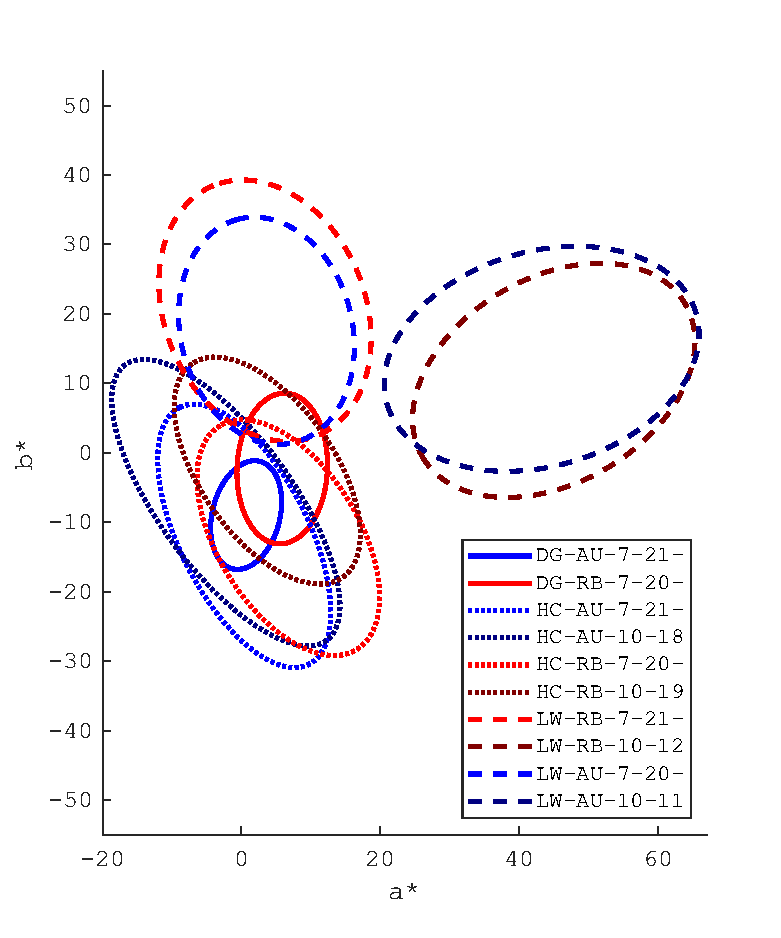
\includegraphics[max width=1.2\textwidth,center]{figs/SmallSphere/SSsummary.pdf}
\caption{A summary of all primary data, in CIELAB}
\label{fig:SSsummary}
\end{figure}

\begin{figure}[htbp]
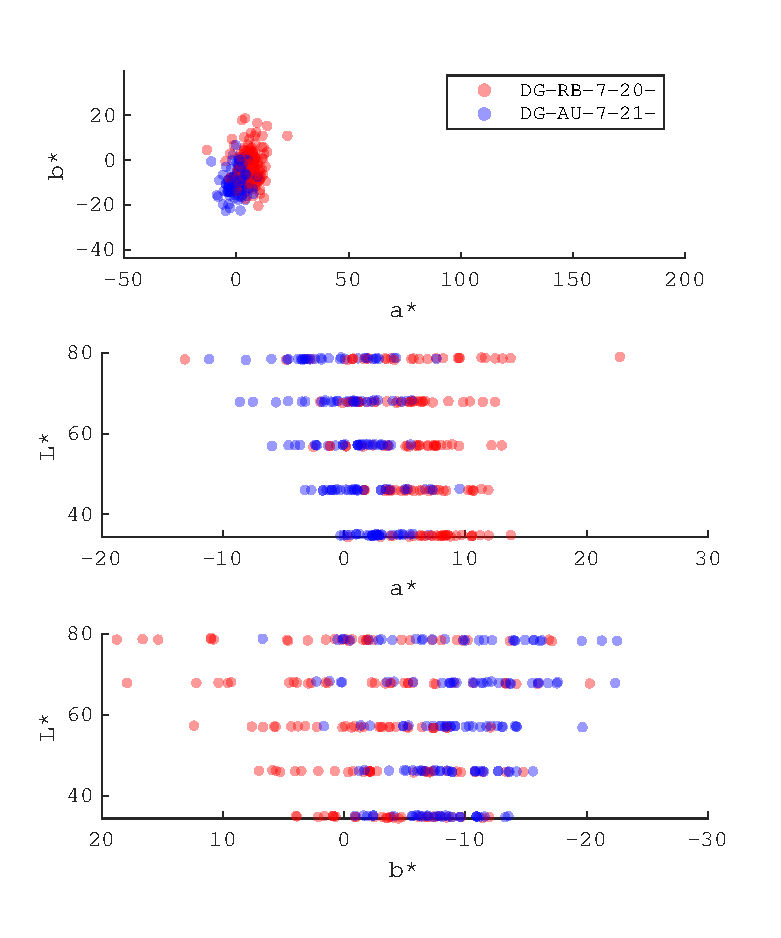
\includegraphics[max width=1.2\textwidth,center]{figs/SmallSphere/DG.pdf}
\caption{}
\label{fig:SS_DG}
\end{figure}

\begin{figure}[htbp]
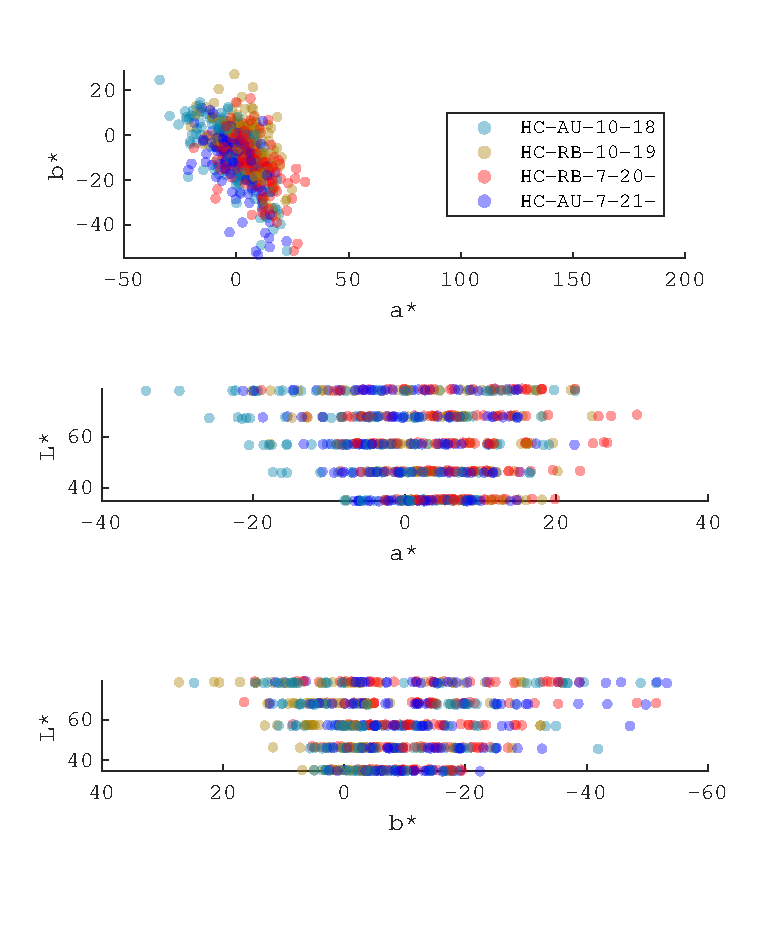
\includegraphics[max width=1.2\textwidth,center]{figs/SmallSphere/HC.pdf}
\caption{}
\label{fig:SS_HC}
\end{figure}

\begin{figure}[htbp]
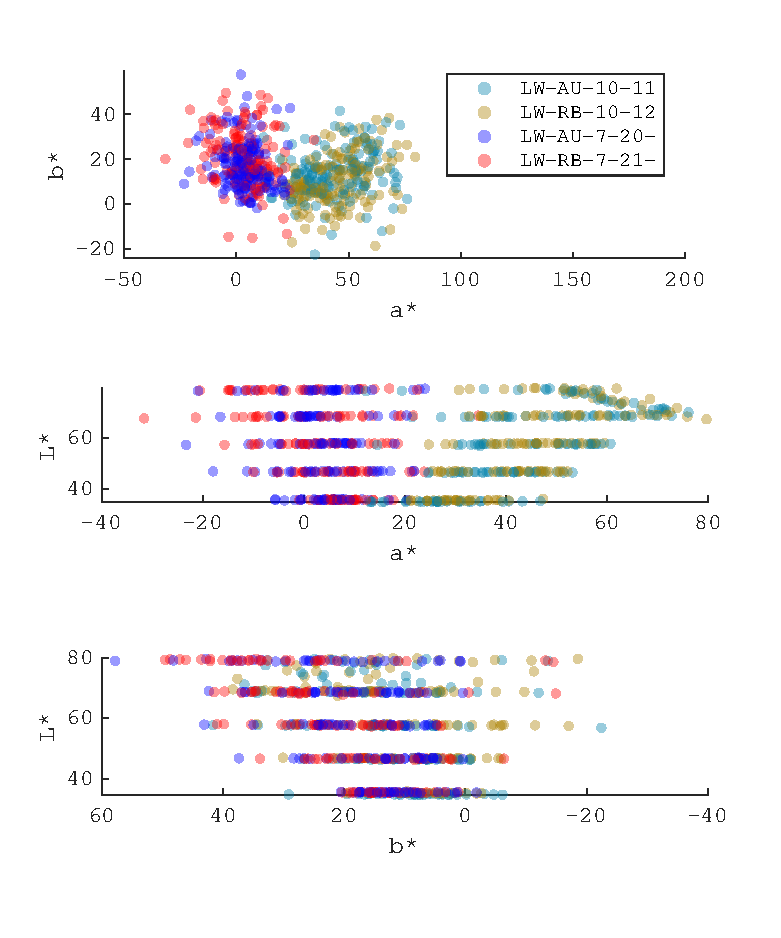
\includegraphics[max width=1.2\textwidth,center]{figs/SmallSphere/LW.pdf}
\caption{}
\label{fig:SS_LW}
\end{figure}

\subsection{Secondary Data}

Data describing the characterisations of hardware follow. Figure \ref{fig:SSLEDs} shows the chromaticities of the adapting surrounds as recording during each session. Figure \ref{fig:SSgamut} shows the recorded gamut and white points of the display measured before or after each session. Figure \ref{fig:SScal2} shows representative results from one of the secondary characterisation sessions.

\begin{figure}[htbp]
%\includegraphics[max width=\textwidth,center]{figs/SmallSphere/SSLEDs.pdf}
\caption{}
\label{fig:SS_LW}
\end{figure}

\begin{figure}[htbp]
%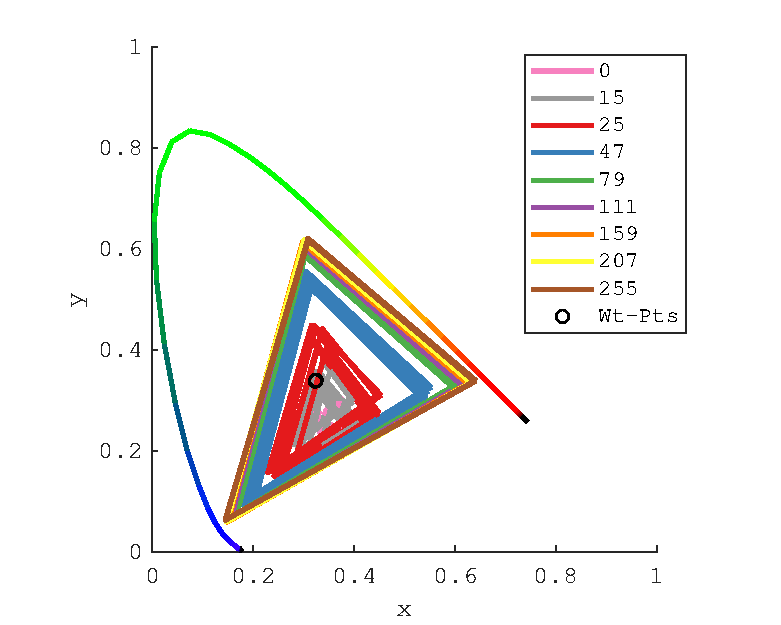
\includegraphics[max width=\textwidth,center]{figs/SmallSphere/SSgamut.pdf}
\caption{}
\label{fig:SS_LW}
\end{figure}

\begin{figure}[htbp]
%\includegraphics[max width=\textwidth,center]{figs/SmallSphere/SScal2.pdf}
\caption{}
\label{fig:SS_LW}
\end{figure}

\section{Discussion}
% Assumptions

%Rod activation
%Calculate melanopic contrast for actual conditions
%Line indicates match

%\chapter{The Spatial Achromatic Point Setting (SAPS) Method}
\label{TabletMethodChapter}

\textit{The work presented here has been presented previously as an oral presentation at AIC 2016 \citep[p. 125]{garside_estimating_2016}\footnote{Abstract available: \doi{10.6084/m9.figshare.4269680.v1}} and as a poster presentation at ECVP 2017 \citep[p. 93]{niko_busch_european_2017}\footnote{Poster available: \doi{10.6084/m9.figshare.5478493.v1}}}

\section{Summary}

The principal aim of this piece of work is to explore a novel method for colour constancy experiments, which allows for experiments to be performed in real and complex environments, in order to better understand colour constancy outside of a lab environment. The \gls{SAPS} method uses a tablet computer to present a spatial version of an achromatic point setting task. 

The key concerns are whether such a methodology can: a) present a stable stimulus across disparate environments, b) record differences in perceptual white point, and c) be suitable for naive observers following minimal instruction. 

On each point, the method is shown to be at least moderately successful, with caveats, and suggestions are provided for improvements upon the current design. Such a methodology could be used to investigate the effect of multiple cues, conflicting cues and cues which cannot easily be reproduced in a lab environment.

Code and data are provided: \url{https://github.com/da5nsy/SAPS/}.

\newpage

\section{Introduction}

To further our understanding of colour constancy, investigators have traditionally designed experiments where the number of variables is greatly reduced compared to a real-world environment. This allows investigators to carefully query the impact of any individual variable, or the interplay of a small number of variables. 

For example, a common stimulus-type used in such experiments are `Mondrian' patterns, arrangements of flat and unmoving overlapping coloured paper rectangles, see Figure \ref{fig:mondrian} \citep{hurlbert_colour_1999}. Consider also the experiments of \citet{kraft_mechanisms_1999} where objects representing potential colour constancy cues such as a tin-foil covered cone (specular highlights) were removed from a neutrally coloured box one-by-one in order to probe their relative usefulness (see Figure \ref{fig:KraftBrainard}).

\begin{figure}[htbp]
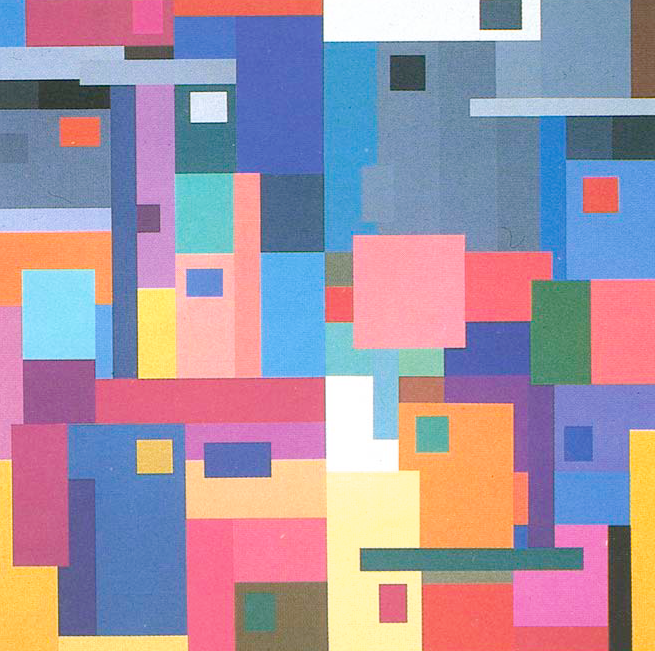
\includegraphics[max width=\textwidth]{figs/tablet/mondrian.png}
\caption{An example `Mondrian', reproduced from \citet{land_recent_1986}.}
\label{fig:mondrian}
\end{figure}

\begin{figure}[htbp]
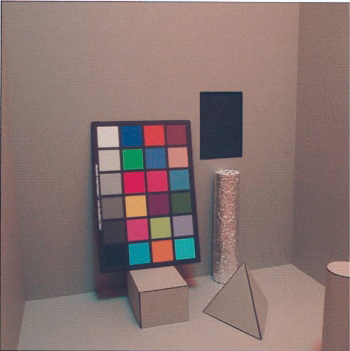
\includegraphics[max width=\textwidth]{figs/tablet/KraftBrainard.png}
\caption{A colour constancy experiment investigating the roles of different potential cues, reproduced from \citet{kraft_mechanisms_1999}. Objects within the scene were carefully selected such that the inclusion or removal or specific objects would allow or exclude the possibility of using a specific mechanism (local adaptation, spatial mean of the image, adaptation to the most intense region) to perform colour constancy.}
\label{fig:KraftBrainard}
\end{figure}

It is clear that these set-ups are much reduced in their complexity compared to a natural scene. Simple experimental stimuli allow for clear questions to be asked, and for those questions to be answered with statistical strength. Such research is valuable. However, the use of simplified stimuli risks overlooking unknown scene attributes, and the human behaviours which may be reliant on them. Experiments often find that colour constancy in lab environments is never `complete'; is this representative of real world behaviour or could this result be due a lab environment failing to deliver all the cues available to an observer in a natural environment? Recent technological advances have enabled experimenters to reproduce natural scenes with increasingly accuracy and comprehensiveness \citep{heasly_rendertoolbox3_2014}, but the number of variables in real scenes is practically infinite, and whilst our ability to reproduce a scene increases over time as technology develops, we only reproduce what we deem important at the time. Using a real-world environment would allow for processes to occur as they do naturally, in the environment for which these processes are presumably optimised (See \citet{kelly_chips_2018} and \citet{shepard_perceptual_1992}). The ability to move away from the lab environment also allows us to run experiments in specific locations of interest, such as museum spaces.

There are two clear challenges to the use of natural environments for scientific study; the inability to control target variables, and the influence of uncontrollable or uncontrolled non-target variables. The first challenge may be surmountable; depending on the variable in question it might either be controlled by force, or over time natural variability may provide the required experimental range. The second may be insurmountable but, depending on the specific situation, it may be permissible to consider uncontrolled variations simply as sources of experimental noise. Further challenges arise where connections exist between target and non-target variables, or where the influence of the non-target variables dwarf the effect of the target variable.

One further challenge: it is rare for an experiment in a real-world environment to not intrude onto that real-world scene and change it in some way. The only true solution to this problem would be to consider unannounced observation of a natural behaviour as the only acceptable scientific method. A pragmatic compromise is to design an experiment such that it modifies the environment of the observer minimally, and to carefully consider the impact that the experimental set-up may have upon observers.

The method presented here is a variant of the `achromatic setting' method.\footnote{For overviews see %section X, or 
the section on `achromatic adjustment' in \citet{foster_color_2011} and `Matching to an internal standard' or `achromatic setting' in \citet{smithson_sensory_2005}.} The achromatic setting method requires an observer, under specific conditions, to adjust the chromaticity of an item in their visual field such that this item appears achromatic. Changes in selected achromatic point (in colour space) are thought to represent general adaptive shifts. For example, an observer in an environment lit by a chromatic illuminant would be expected to pick an achromatic point which is shifted towards the chromaticity of the illuminant, compared to the achromatic point which they might select in a more neutral environment. This is often practically achieved by having the `object' be an area of a computer screen, and have it controllable in two or more chromatic dimensions (such as relative amounts of unique red/green and blue/yellow). 

In the \gls{SAPS} method, as presented here, a tablet computer is given to an observer to hold as is comfortable to them, and upon this computer an isoluminant slice through a nominally perceptually uniform colour space is presented, from which they are requested to select (by touching upon the screen with a finger) the point which they deem to be most achromatic (the specific phrase `grey-est or least colourful' is employed in order to make the task suitable for non-colour-scientist observers). The term `spatial' is used since the user provides information by making a spatial selection which directly corresponds to a colour choice, where in other methods abstract sliders or knobs may be used to alter the chromaticity of a static object.

To minimise the effect of the presentation of chromatic scenes upon the viewer, which may influence an observer's state of chromatic adaptation, this process is repeated a number of times with the area of colour space which is presented varying, through random rotation about the luminance axis, and random offsetting through both dimensions of the chromatic plane.

In the rest of this chapter I will describe the method in more detail, and describe some experiments performed to explore the potential abilities and limitations of such a method.

\section{Research Questions and Hypotheses} \label{sec:qandhyp}

\subsection*{Hypothesis 1: The \gls{SAPS} method is suitable for colour constancy experiments}

To be fit for performing colour constancy experiments, this method needs to:

\begin{enumerate}[label=\Alph*.]
    \item \label{list:hyp1a} \emph{Provide a relatively environment-agnostic stimulus.} 
    This experimental method relies on the assumption that the tablet display delivers a stimulus with identical physical properties to the observer independent of environment, with no effect of ambient illumination. In practical terms, this means that the tablet must not be affected by reflection, either at the glossy surface of the tablet display, or at reflection at any other level of the display architecture, to the extent that this has a non-negligible impact upon recorded data. If it is found that this is not the case, the tablet would need to be characterised separately for each environment.
    \item \label{list:hyp1b} \emph{Collect meaningful data.} 
    One would expect this to be indicated by small intra-observer variability (not recording a change where there is presumably none), and reasonable inter-environment change (recording a change where there is presumably a change). It would be expected that these changes would be in line with previously published results.
    \item \label{list:hyp1c} \emph{Additional aim - Be suitable for naive\footnote{In this instance by `naive' I mean non-colour-scientist (a large number of colour vision experiments have been run only with colour scientists as observers and it is possible that this has biased results) and untrained (it is relatively common for this type of experiment to require extensive training upon a colour naming system such as The Munsell System of colour, by which participants are asked to report the appearance of a test object)} observers.}
    This would reduce the amount of time and effort required to run experiments, and allow for the collection of data from participants less likely to be biased through task expectation. It also means that the demographic group of observers is less likely to be 
    WEIRD (`Western, Educated, Industrialized, Rich, and Democratic', \citep{henrich_weirdest_2010,brookshire_social_2013,justsaysinweird_just_2019}), white, and undergraduate.
\end{enumerate}

\subsection*{Hypothesis 2: \gls{ipRGC} activation affects perceptual white point.}
Primarily as a proof of concept for this methodology, but also to assist in answering other research questions posed within this thesis, an experiment was performed whereby observers made achromatic selections under a selection of colorimetrically metameric illuminants where there was a melanopic contrast between illuminants. %See section X. 
If \gls{ipRGCs} play a role in colour constancy we would expect to see a distinction between the responses recorded under the different illuminants. 

\section{Experimental set-up and methodology}
\subsection{Method \& Apparatus}

\subsubsection{Selection of participants}

The participants for experiment 1 were the author, one of the author's academic supervisors (KC) and a technician at the laboratory (TS).

For experiment 2, 58 observers were selected randomly from museum visitors. A visitor would be approached by the experimenter (the author) and asked whether `they would be interested in taking part in a colour vision experiment'. Those who replied positively were verbally informed of the ethics details for the study, the principal parts of which were: that no identifying information would be recorded, that the experiment carried no risks greater than those associated with normal use of a tablet computer, that observers were not paid or otherwise incentivised to take part, and that the task would take roughly ten minutes. A verbal description of the ethics details for this experiment was provided rather than the more normal paper version to avoid providing the observer with a white reference immediately prior to the experiment. This study was approved by the \gls{UCL} Ethics committee (Project ID Number: 9357/001). In accordance with the ethics approval granted for this project, people under the age of 18 were only invited to participate under the supervision of a parent/carer. %[Appendix X] !!!!!!!!!!!!!
% number, age and sex here

For experiment 3, nine participants (5 female, 4 male, ages not recorded) were recruited from the author's friends and family (including one academic supervisor), with the hope that this would assure attendance and motivation and to take advantage of short-notice availability of the experimental space. Participants were informed of the ethics details for the study in advance of attending. Ethics approval was provided following the amendment of the aforementioned ethics application (9357/001).
% number, age and sex here

\subsubsection{Instructions to the participants}

The observer was instructed to hold the tablet such as was comfortable for them to do so, upon which the first trial of the experiment was already visible. They were instructed to `touch the grey-est, or least colourful, point on the screen'. Upon touching the screen, the stimulus would be replaced with a new stimulus. This new stimulus was a new subsection of the full stimulus image (See Figure \ref{fig:Stimulus}) which had been randomly rotated and offset (further information provided in Section \ref{sec:stimuli}).

\begin{figure}[hbtp]
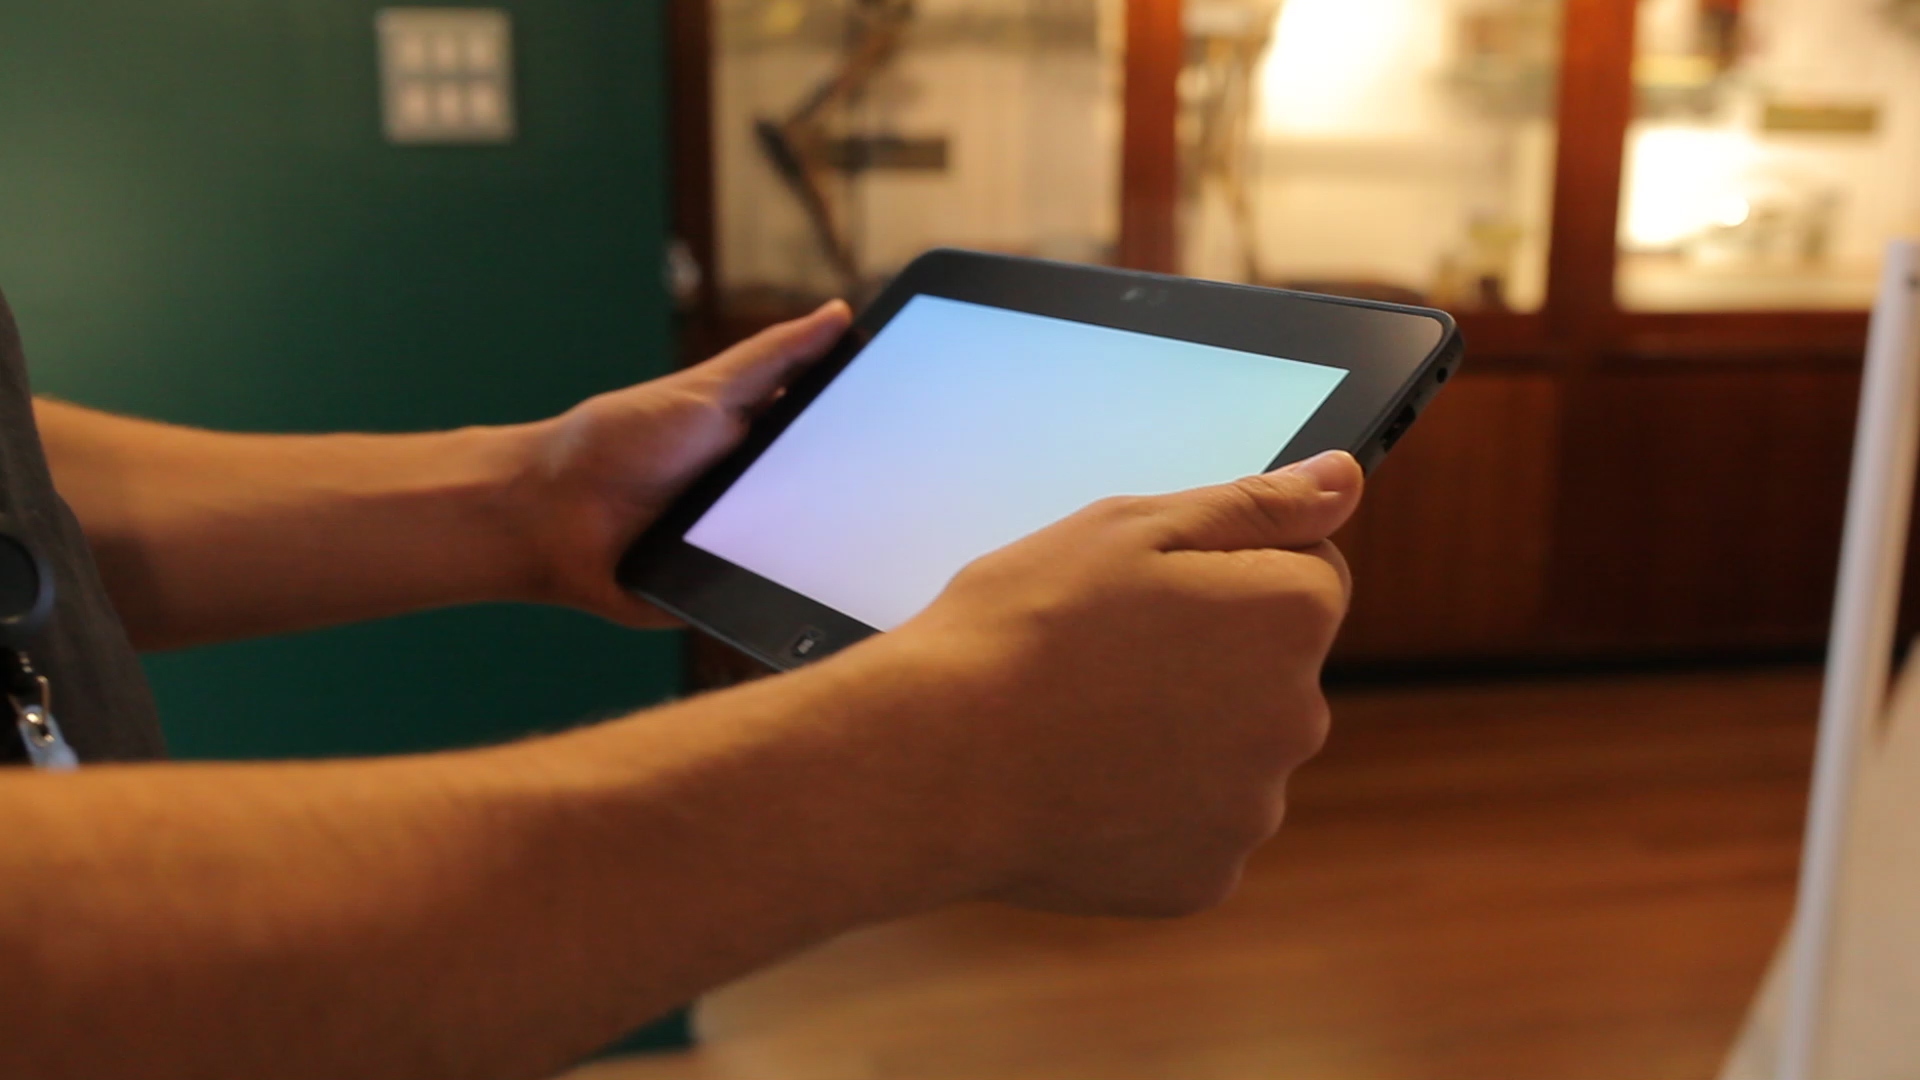
\includegraphics[max width=\textwidth]{figs/tablet/MVI_3213-1.jpg} % E:\Pictures\2016\2016-10-14
\caption{A participant (the author) holding the tablet with a stimulus on screen.}
\label{fig:grant_demo}
\end{figure}

Most observers seemed to find this task difficult for the first stimulus (appearing confused and often verbally expressing difficulty), but within the first few stimuli seemed to develop an increased comfort and ease with the task, which resulted in a decreased response time. %(Illustrate with graph of response time?)
At this point the observer was told that there would be thirty trials. No training was provided, and no runs were excluded as training runs. One stimulus was forced to have identical rotation and offset to an earlier stimulus, in order to assess intra-observer variation (see Section \ref{sec:exclusion}).

\begin{figure}[hbtp]
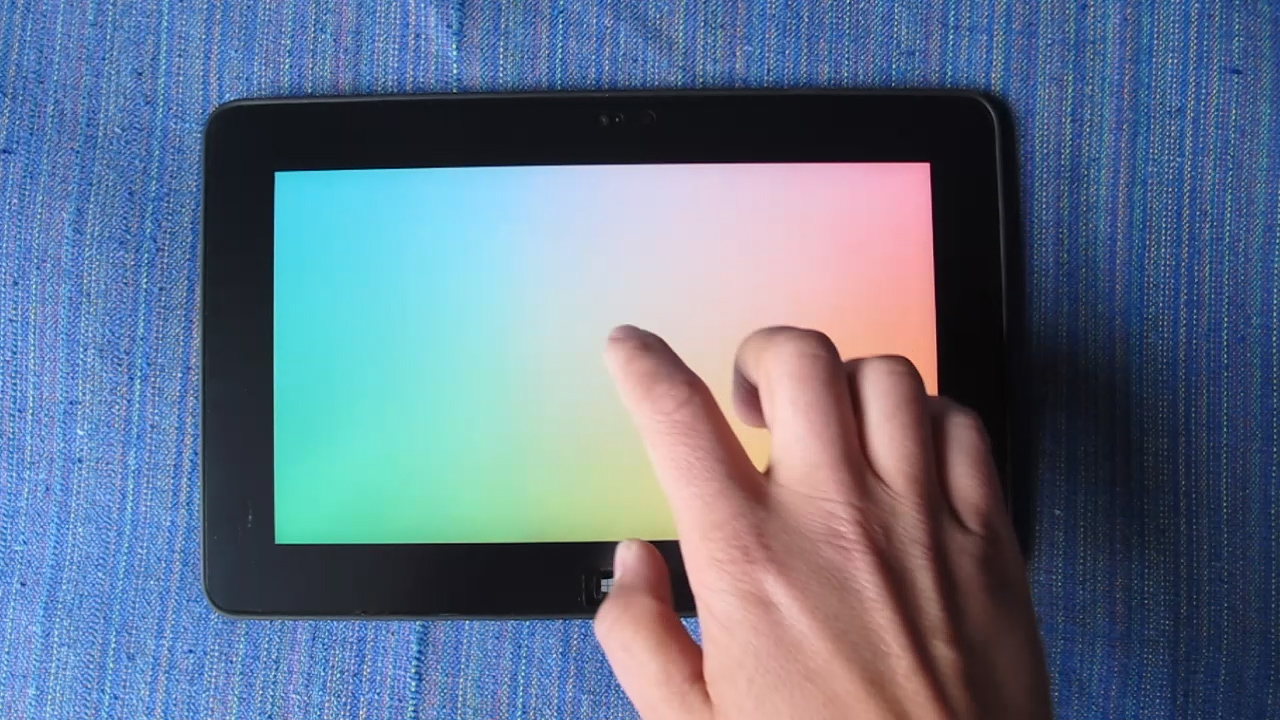
\includegraphics[max width=\textwidth]{figs/tablet/MVI_3889-4.jpg} % E:\Pictures\2016\2016-10-18
\caption{A stimulus displayed upon tablet and finger in motion towards subjective point of achromacy.}
\label{fig:finger}
\end{figure}

Following the thirty trials, a secondary task was presented to observers, designed to characterise their touch input. This task features a 2x2 checker board pattern upon a black background (See Figure \ref{fig:checker-board}). Observers were instructed to touch the centre of this checker board. Upon registering a touch, a new checker-board would be presented, of the same attributes but modulated in position in the same way as the main stimulus. This stimulus is presented 10 times. This data was later used to calibrate touch input, and to ascertain the amount of measurement uncertainty derived from touch input. 

\begin{figure}[hbtp]
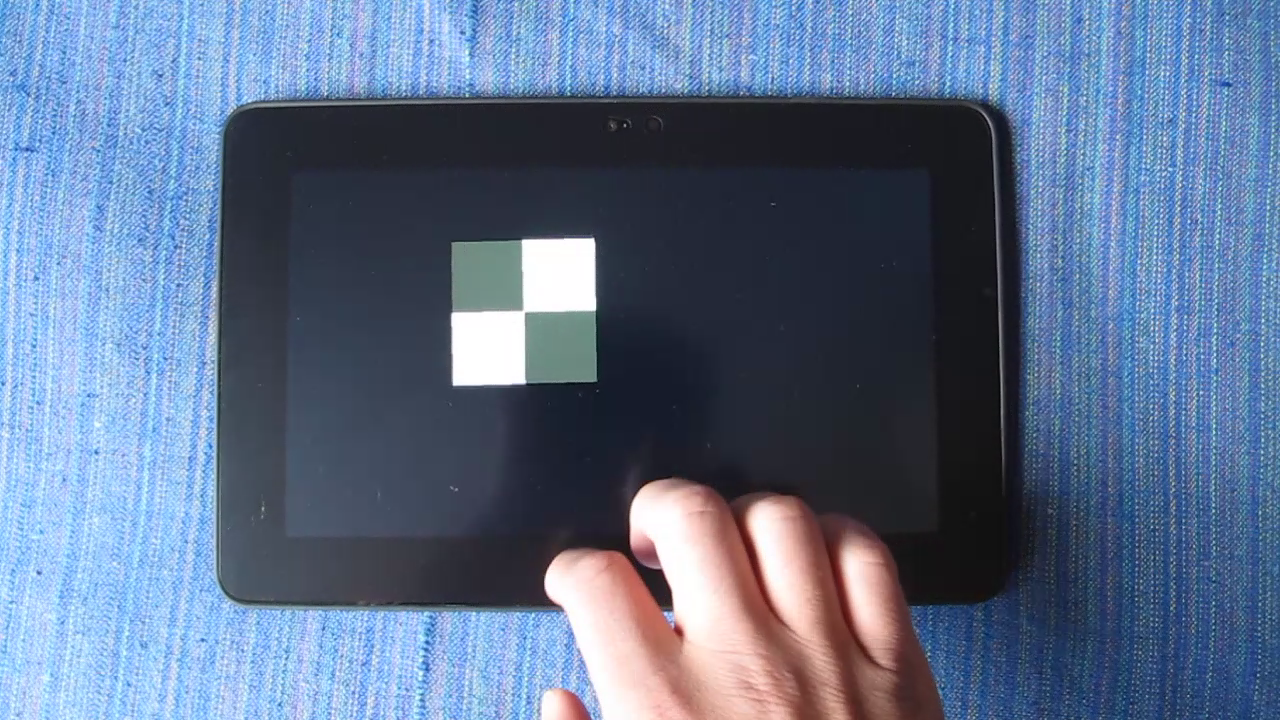
\includegraphics[max width=\textwidth]{figs/tablet/checker_board.png} % E:\Pictures\2016\2016-10-18
\caption{Photo of checker-board task. Participant is requested to touch centre of the checker-board pattern.}
\label{fig:checker-board}
\end{figure}

%Doing this without incentive for participants meant that it was rushed (?)

\subsubsection{Specification of tablet PC}

Participants undertook the experiment upon a Dell Latitude 10 ST2 tablet computer with `BROTECT' Matte Screen Protector (223x126mm active screen area, 1366x768 pixels). This tablet was chosen for its ability to run a Windows environment, and the matte screen protector was added to reduce the severity of specular reflections. The measured gamut of this device is shown in Figure \ref{fig:gamut}, with the gamut of sRGB for comparison.

\begin{figure}[hbtp]
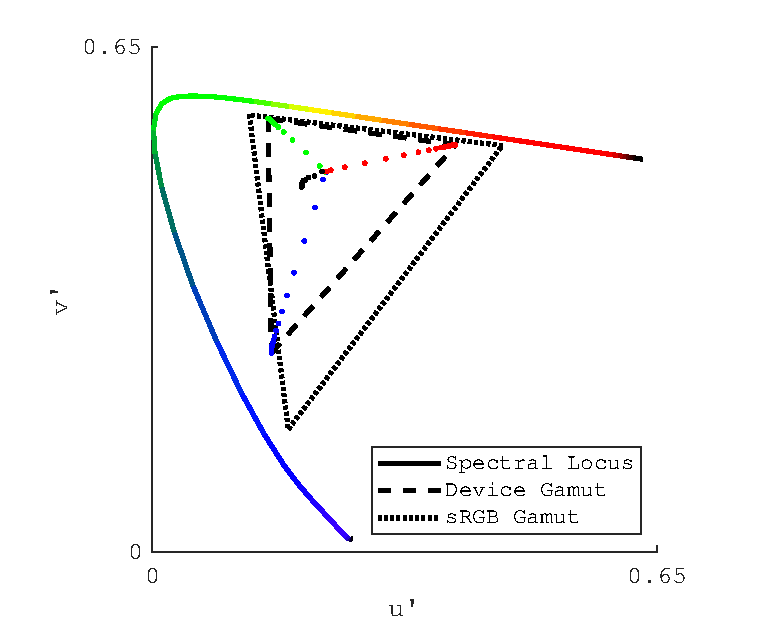
\includegraphics[max width=\textwidth]{figs/tablet/gamut.pdf}
\caption{The display gamut, plotted in CIE u'v' space. Red, green and blue dots indicate chromaticities of single channels at pixel values from 0 (central values) to 255 for each respective channel. The black dots are the chromaticities achieved when the pixel values are kept in line for each channel. This can be described as the native white point of the display, and can be seen to drift leftwards and then downwards as pixel values increase.}
\label{fig:gamut}
\end{figure}
% Generated using the 'Plot gamut' section of SAPS_TabletCharacterisation.m

\subsubsection{Selection of colour space for creating the stimuli}

The stimulus presented to observers was an isoluminant plane (in CIE L*) through CIELUV colour space. CIELUV was chosen for having an associated object colour space, where comparisons between the chromaticity of light sources and the chromaticity of selections could be made. 

\subsection{Stimuli} \label{sec:stimuli}
\subsubsection{Generating the stimuli}

The stimulus was specified as: L*: 60 uniformly across field, u*: ranging linearly from -50 to 50 from one side of the field to the other, and v*: as for u*, but along the orthogonal axis, so that the stimulus was of uniform lightness and smoothly changing hue and chroma. The full stimulus image (Figure \ref{fig:Stimulus}) was 2188 pixels square; this is larger than the pixel dimensions of the screen to allow for the stimulus to be rotated freely and offset by up to a third of the image in any direction before the edge of the image is encountered. 

The stimulus was specified with the above attributes in a matrix within \gls{MATLAB}\footnote{Code: \url{https://github.com/da5nsy/SAPS/blob/21940bb6ed9d0e37d88e1b655f4919d73431743a/experiment/stimulusGenerator002.m}}. CIELUV values were converted to XYZ tristimulus values using built in functions, with reference white set as the XYZ tristimulus values of the display at maximum white (with screen protector), as measured with an Xrite i1 device (shown in Figure \ref{fig:gamut}). Linearisation was achieved through the use of a look-up table, computed by spline interpolation of the measured outputs at 15 pixel %(KT: pixel drive value?)
value increments from 0 to 255 for each channel. The stimulus was then output as an 8-bit tiff image, which could be easily loaded and manipulated by the psychophysical stimulus presentation software PsychoPy \citep{peirce_psychopypsychophysics_2007}. %(Illustrate with flow diagram?)

\begin{figure}[hbtp]
\includegraphics[max width=\textwidth]{figs/tablet/stimulus.png}
\caption{Full stimulus image, from which subsections were selected and presented as stimuli. Note that no effort has been made to correct this image for printing, and so it is best considered as only a rough approxmation.}
\label{fig:Stimulus}
\end{figure}
% Copied and pasted from original psychopy folder. Could regenerate using stimulusGenerator002.m

\subsubsection{Presenting the stimuli}
A program was written in PsychoPy\footnote{\url{Code:  https://github.com/da5nsy/SAPS/blob/21940bb6ed9d0e37d88e1b655f4919d73431743a/experiment/SpatialAchromaticPointSetting_0940_Grant.py}} that presents the stimulus 30 times, with random rotation and random offset in the horizontal and vertical dimensions of between -1/6 and +1/6 of the respective dimension. Thus `objective grey', where [u*,v*] = (0,0), was always within the central third (in each dimension) of the screen. This program saved details of the stimulus offset and rotation (`dpX', `dpY' and `ori'), co-ordinates of observer selected point (`x-co\_raw', `y-co\_raw', and also `direction\_raw', `magnitude\_raw'), and time taken to make selection, measured since last selection (`toc\_raw').

The effect of rotation and offset was such that on each stimulus presentation the observer saw a stimulus that appeared somewhat different to the previous stimulus, but still hopefully included their preferred achromatic point. The rotation and offset can be illustrated by plotting the chromaticities present in any one stimulus presentation, as in figure X. %!!!!!!!!!!!!!!!!!!!
Plotting the chromaticities present across a full run of 30 trials yields Figure \ref{fig:practical}, where it can be seen that the rotation results in a roughly circular spread of chromaticities, and the rotation and the offsetting together result in a gradient of likelihood of presentation which is high at the centre of the full stimulus and lowest at the edges of the full stimulus. This gamut distribution is referred to further in the text as the `practical gamut'.

% Single shot figure needed

% \begin{figure}[hbtp]
% \includegraphics[max width=\textwidth]{figs/tablet/????}
% \caption{A representation of the chromaticities present in a single stimulus. Note that the gamut is not rectangular for 2 reasons: firstly, because CIELUV is not a linear transformation of CIE u'v' , and secondly because for this particular stimulus, the bottom left corner (as presented above) intersects with the display gamut boundary, resulting in a gamut compression to that corner.}
% \label{fig:?????}
% \end{figure}


\begin{figure}[hbtp]
\includegraphics[max width=\textwidth]{figs/tablet/practical_gamut.pdf}
\caption{The `practical gamut'. This plot shows the relative frequency that chromaticities are actually presented, within the boundary of the device gamut (as shown in Figure \ref{fig:gamut}). The highest number of times a particular chromaticity can be presented is 30, since there are 30 trials in a typical run. As described in the main text, chromaticities falling towards the specified objective white point of the stimulus are presented every stimulus, whereas those further away from the centre of the stimulus are presented less frequently. On the left-hand side of the cluster it can be seen that the gamut boundary is reached. This is discussed further in section X. %!!!!!!!!!!!
}
\label{fig:practical}
\end{figure}


\subsubsection{Touch input characterisation} \label{sec:touch}
The checker-board stimuli (Figure \ref{fig:checker-board}), included to allow for fine spatial calibration for individual observers' touch input, was generated by running the main experimental script again but with the stimulus file path replaced with a simple pattern generated within PsychoPy.

I hypothesise that any shifts in touch input would be the result of one or both of two potential influences: personal finger offset and general hardware calibration. By the former I refer to the fact that whilst a finger is considered to be a relatively discrete unit, controlled with presumed dexterity and accuracy, the specific part of the finger which touches the screen will vary from person to person, with each person exhibiting a reliable bias. By the latter I refer to the fact that it is highly possible for there to be a `fairground gun effect', whereby the hardware introduces a reliable bias due to calibration misalignment, which affects every observer equally.

Performing a calibration of each observer's data based on this individual characterisation allows for offsetting of both of these types of variation. 

\subsection{Data Analysis}
\subsubsection{Processing Pipeline}

The data was analysed in \gls{MATLAB} using the following pipeline:
\begin{enumerate}
\item Data loaded into \gls{MATLAB} from an excel file
\item Spatial touch points calibrated using touch characterization data
\item Spatial data converted into chromaticity data
\item Data graded for performance and exclusions applied where appropriate (see Section \ref{sec:exclusion} for further details) 
\item Data plotted either as:
\begin{enumerate}
\item Full dataset scatter %!!!!!!!
\item Standard deviation ellipse/line plotting\footnote{Based on code from: \url{https://stackoverflow.com/a/3419973}}.%!!!!!!!
\item Dataset mean plotting (only where number of participants was large)%!!!!!!!
\end{enumerate}
\end{enumerate}

\subsubsection{Exclusion Criteria} \label{sec:exclusion}

In this task, a `good' performance is one where it seems an observer understood the given instructions well, and was able to act upon them. Such a performance should be indicated by data which suggests that an observer was able to repeatedly select their chosen chromaticity in spite of the spatial relocation of this chromaticity during the experiment. It is expected that observers will perform with differing levels of competence, due to a variety of reasons, e.g.: level of commitment/interest, visual/pointing ability, understanding of the task. It seems reasonable to exclude data that indicates that an observer performed `less well' than a determined threshold.

A measure of performance could be computed by measuring variance in a dataset for each observer. In an ideal situation, an observer would select precisely the same chromaticity on each trial, and so the variation would be 0. More realistically, slight variance is expected, due to input imprecision, fuzzy boundaries of acceptability and `smearing' artefacts (see Section \ref{sec:bounding}).

Two simple methods for assessing this variability are readily available. The first involves calculating the average standard deviation of data for each observer; either considering a single chromatic axis, both axes, an average of both axes, or considering a newly defined axis such as the axis of greatest or least variability. The second involves comparing data from unannounced repeat stimuli (within each observation run trials 3 and 8 were identical, and if an observer was performing the task effectively the difference in records for these two stimuli should be minimal). This second method shall be referred to as \acrfull{DBUR}.

The first method has the advantage that it considers the entirety of each dataset; whereas the second method requires that general assumptions about the entirety of an observer's data be made from only two data points. One disadvantage of the first method however, is that this measure would give a high value in the situation that there was a moderate or higher level of `smearing', since increased spread could result from a situation where an observer was very good at selecting their chosen chromaticity, but was unable to do so since that chromaticity was not always displayed. In contrast, the second method should be unaffected by this.

A further advantage of the first method is that a non-arbitrary threshold presents itself; that of the level of variability which would result from a run of the experiment where a hypothetical observer selected the exact same physical point on the screen for each stimulus. This would represent the best possible performance of an observer who was unable, or had no interest in, following a specific chromaticity, though of course it would not include any variability attributable to a touch input (though this could be artifically simulated). The second method presents no such intuitive definition for a threshold.

\begin{table}[hbtp]
\begin{tabular}{|p{0.5\textwidth}|p{0.5\textwidth}|}
\hline
\emph{Standard Deviation} & \emph{\acrshort{DBUR}} \\
\hline
Considers entire dataset & Requires generalisation from only two points per observer \\
\hline
Susceptible to `smearing' artefacts & Not affected by gamut boundary issues \\
\hline
Intuitive threshold: the SD of a `baseline' observer & No intuitive threshold \\
\hline
\end{tabular}
\caption{Comparison of exclusion criteria options.}
\label{tab:exclusion}
\end{table}

%figure

%Reinclude later: 

% In figure X `Mean SD' (SD from now on) is calculated for each observer's data by taking the mean of the standard deviation in the u' and v' chromatic dimensions. \gls{DBUR} is calculated as the two-dimensional Euclidean distance between the two chromaticity coordinates for the two identical stimuli.

% It can be seen that on both measures there are a small number of clear outliers; a group of three points with SD around 0.02 but very low \gls{DBUR}, and two points with very high \gls{DBUR}. Using only one of these two measures would fail to pick up some of these points, though as a single measure SD would be more effective in recognising these points.

% A vertical line is plotted from the point representing baseline data. This data is calculated by computing the results for a hypothetical observer who pressed the precise centre of the screen for each stimulus, and the precise centre of the checker-board on the touch characterisation phase. 

% As can be seen from this line, a threshold based on this measure would exclude a very large number of datasets. This is partly due to the fact that most real observer's exhibit orientation-dependent variability, with the greatest axis of variability generally being in line with the cerulean line, whereas the hypothetical data is theoretically rotationally symmetrical. It may be more appropriate then to compare the SD of the hypothetical dataset to the SD of the axis of least variability for real data. However, this could be seen as being overly lenient towards the real data. As a compromise, and for simplicity, let's consider the minimum value between u' SD and v' SD (rather than the mean) as the representative for real data, which shifts relative positions of the data and the threshold such that more datasets pass this test. 

%figure
%--------%

% I don't really do stats here...
% \subsubsection{Statistical Analysis}

% Data was considered in comparison to a baseline dataset, consisting of the results of a theoretical trial where an observer touched the spatial centre of the screen each time %(further details in section 5.1), 
% and a practical gamut which describes the frequency with which each chromaticity was presented to the observer. %!!!!!!!!!!! (See section 3.1 for further discussion of this).
% %Demo plots?

\subsection{Environments}

\subsubsection{\gls{UCL} \acrshort{PAMELA}} \label{sec:PAMELA}

\gls{UCL}'s \acrfull{PAMELA} consists of a large open space, enclosed within a light-proof warehouse, and is most often used for its customisable floor space, where small sections can be independently raised or lowered to recreate the spatial configurations of public spaces such as streets or railway platforms (see \citet{cheng_effect_2018} for example, and Figure \ref{fig:PAMELAobs1}). It is of interest to this project since it also has a customisable lighting rig comprising 44 addressable fixtures, each with 6 independent channels, which is controlled via a PC interface, and an additional high power white channel, which is on a separate control system. 

\begin{figure}[hbtp]
\includegraphics[max width=\textwidth]{figs/tablet/PAMELAlights1.jpg}
\caption{The fixtures mounted on the ceiling lighting rig at \acrshort{PAMELA}. Photo credit: Keats Webb.}
\label{fig:PAMELAlights1}
\end{figure}

\begin{figure}[hbtp]
\includegraphics[max width=\textwidth]{figs/tablet/PAMELA_SPD.pdf}
\caption{\gls{SPD} of the 7 different channels available in the \gls{PAMELA} lighting rig.}
\label{fig:PAMELAlights2}
\end{figure}

\begin{figure}[hbtp]
\includegraphics[max width=\textwidth]{figs/tablet/PAMELA_screenshot.jpg}
\caption{The control panel for the LED rig at \gls{PAMELA}.}
\label{fig:PAMELAlights4}
\end{figure}

For experiments reported here three illumination settings were defined - `Cool White (`CW')', `Warm White (`WW')', and `Mel-High (`MH')'. \gls{SPD}s are shown for each in Figure \ref{fig:PAMELAlights5}, and chromaticities in \ref{fig:PAMELAlights6}. `CW' and `WW' were system defaults, and `MH' was defined to be a colorimetric match (for the CIE 1931 observer) for `CW', but preferentially using an \gls{LED} band with a peak spectrally close to the peak spectral sensitivity of melanopsin ($\sim$480nm).

\begin{figure}[hbtp]
\includegraphics[max width=\textwidth]{figs/tablet/PAMELA_SPD.png}
\caption{\gls{SPD}s for the different illumination settings at \gls{PAMELA}. \hl{Will reformat, add legend and add axis labels}}
\label{fig:PAMELAlights5}
\end{figure}

It should be noted that luminance was not matched between the conditions. Therefore, `CW' and `MH' could be described as colorimetric matches, but not as metameric matches. Additionally, for chromatically distinct conditions (`CW' vs `WW'), there is a confound of luminance variation. The luminances of the three conditions were 235lx, 720lx and 840lx respectively. In the opinion of the author, it would be advisable that if further studies of this type were undertaken, that conditions be matched for luminance in order to discount this as a variable. 

The chromaticities of the light sources, measured with a UPRtek MK350, were:
`WW': 	u'v'(0.248,0.524) (averaged over 4 measurements);
`CW': 	u'v'(0.200,0.465) (averaged over 3 measurements);
`MH': 	u'v'(0.201,0.467) (averaged over 8 measurements).

\begin{figure}[hbtp]
\includegraphics[max width=\textwidth]{figs/tablet/PAMELA_chromaticities.pdf}
\caption{Chromaticities of defined lighting conditions at \gls{PAMELA}. Note that `CW' and `MH' overlap.}
\label{fig:PAMELAlights6}
\end{figure}

\subsubsection{The British Museum} \label{sec:BM}

The British Museum is a large museum located close to the main \gls{UCL} campus, which exhibits artefacts of artistic, cultural and historical relevance. It is one of the UK's most visited tourist attractions, drawing over 5 million visitors yearly \citep{simon_calder_tate_2019}.

\medskip \noindent
Three spaces within the museum were used (with permission):

\begin{itemize}
    \item Rooms 77/78 (`Greek and Roman Architecture', `Classical Inscriptions'), lit with fluorescent lighting.
    \item Room 25 (`Africa' - specifically the east section of the room), lit with tungsten  lighting.
    \item The Queen Elizabeth II Great Court (referred to as `GC'), lit with filtered daylight \citep{foster_and_partners_london._great_2002} during daylight hours, with additional lighting at twilight and after sunset. All experiments were carried out during daylight hours, where additional artificial lighting was not employed.
\end{itemize}

\begin{figure}[hbtp]
\includegraphics[max width=\textwidth]{figs/tablet/BM_SPD.pdf}
\caption{\gls{SPD}s for the environments used at the British Museum.} 
\label{fig:BM_SPD}
\end{figure}

\begin{figure}[hbtp]
\includegraphics[max width=\textwidth]{figs/tablet/BM_Africa.jpg}
\caption{Photo of the author explaining the experiment to an observer at the British Museum. Permission to reproduce image gained from the member of public. Photo credit: Mona Hess.}
\label{fig:BM_Africa}
\end{figure}

\begin{figure}[hbtp]
\includegraphics[max width=\textwidth,max height=0.7\textwidth]{figs/tablet/BM_GC.jpg}
\caption{Photo of the author performing the experiment in GC. Photo credit: Lindsay MacDonald.}
\label{fig:BM_GC}
\end{figure}

\begin{figure}[hbtp]
\includegraphics[max width=\textwidth,max height=0.7\textwidth]{figs/tablet/BM77.jpg}
\caption{Gallery 77, with fluorescent tube illuminantion. Photo credit: \url{https://sites.google.com/site/jwmuseumbibletours/all-artefacts/037-temple-of-artemis-at-ephesus}}
\label{fig:BM77}
\end{figure}

These three galleries are lit with different lighting technologies of distinct chromaticities, though Room 77/78 and Room 25 are both strongly yellow, as shown in Figure \ref{fig:BMchromaticities}.

\begin{figure}[hbtp]
\includegraphics[max width=\textwidth]{figs/tablet/PAMELA_chromaticities.pdf}
\caption{Chromaticities of lighting conditions at The British Museum.}
\label{fig:BMchromaticities}
\end{figure}

\subsubsection{\gls{UCL} Chadwick Building}

Additional testing was undertaken within the Chadwick Building of \gls{UCL} (home of the Department of Civil, Environmental and Geomatic Engineering), in light-tight basement rooms fitted with fluorescent lighting.

% \subsubsection{\gls{UCL} Grant Museum of Zoology}

% The \gls{UCL} Grant Museum of Zoology is a natural history museum within \gls{UCL} with over 68,000 specimens, which is open to the public and also used as a teaching resource. It is lit with a mixture of daylight and \gls{LED} lighting, and a rarely used fluorescent lighting system (not used during any experiments).
% This space was used for preliminary experiments. 

% \begin{figure}[hbtp]
% \includegraphics[max width=\textwidth]{figs/tablet/grant.jpg} 
% \caption{The central space at the \gls{UCL} Grant Museum of Zoology. Note the daylight on the left, the \gls{LED} lighting at mid-height and the fluorescent lighting at the very top of the image. Image copyright: \gls{UCL} and Matt Clayton.}
% \label{fig:grant}
% \end{figure}

\clearpage

\section{Experiments}

\subsection{Experiment 1}
%PAMELA, DG, 13 runs
With the goal of understanding both the intra/inter-observer variability and intra/inter-environment variability, 13 runs of the experiment were performed by the author under the 3 illumination settings defined at \gls{PAMELA} (see Section \ref{sec:PAMELA}), 4 under `WW', 6 under `CW', 3 under `MH', after 2 different lengths of adaptation (5 minutes and 30 minutes). In initial analyses no effect of length of adaptation was found, and so we group the data across these 2 conditions for analysis. Two other observers (KC and TS) also performed a number of observation (3 and 4 respectively) under a range of illumination settings.

\subsection{Experiment 2}

Extending the above experiment, particularly to the inclusion of naive observers, an experiment with a 58 observers was performed at \hyperref[sec:BM]{The British Museum}. See Figures \ref{fig:BM_Africa} and \ref{fig:BM_GC}.
The experiment was performed over five days, during which participants made observations in one of three gallery spaces. The three galleries used were Room 77/78, Room 25 and The Queen Elizabeth II Great Court, as described in section \ref{sec:BM}. 

\subsection{Experiment 3}
In order to provide a case study for this methodology, and to investigate the role of melanopic activation upon achromatic settings, an experiment was performed at \gls{PAMELA} (see Section \ref{sec:PAMELA} for details), under the 2 of the 3 lighting conditions previously defined (`CW' and `MH'), with a repeat of `MH'. A reminder: these two lighting conditions which were specified to be colorimetrically matched for the CIE 1931 observer, but with differing melanopic flux. In this experiment, the condition previously referred to as `CW' shall be referred to as with `ML' (for `mel-low'), for clarity in order to align with current literature.

The null hypothesis for this experiment is: achromatic settings are determined solely by retinal cone catches. A corollary of this is that melanopic flux plays no role. CIE 1931 chromaticity is used as a proxy for retinal cone catches.

%table

%figure

%figure

After entering the main space at \gls{PAMELA}, the space being illuminated solely by the \gls{LED} rig in `MH' mode, and after a minimal adaptation period (5 minutes) during which introductions and instructions were given, individually performed the experimental task in succession. 

\begin{figure}[p]
\includegraphics[width=\textwidth]{figs/tablet/PAMELAobs1.jpg} 
\caption{The experimental set-up at \acrshort{PAMELA}. Left: an observer performs the experiment. Right: other observers wait for their turn to perform the task.}
\label{fig:PAMELAobs1}
\end{figure}

\begin{figure}[p]
\includegraphics[width=\textwidth]{figs/tablet/PAMELAobs2.jpg} 
\caption{The experimental set-up at \gls{PAMELA}. An over the shoulder shot of an observer performing the task.}
\label{fig:PAMELAobs2}
\end{figure}

Once each observer had performed the task once, the lighting was changed to `ML' lighting condition, and the observers again performed the task in succession. Finally, the lighting condition was returned to the initial state (`MH', referred to from now on as `MH2' to indicate that it is a repeated measure) and participants once again performed the task. Information about the nature of the lighting conditions was not provided to participants, though the change was noticeable, and observers were not informed that the third condition was a repeat of the first condition. 

When not performing the task, other participants were seated facing away from the participant currently performing the task, so as not to put pressure on the participant performing the task, and to ensure that observers were not influenced by the tactics or choices of other participants. Participants were instructed not to use phones or other electronic or light emitting devices for the duration of the experiment, but were encouraged to engage in discussion with other participants. The order in which participants performed the task was decided by the author, in an arbitrary but not properly random manner. This order was then maintained for each set of observations (the observer who performed the task first under the first condition also performed first under the second and third conditions, etc.).

Participants were not tested for colour-anomalous vision since it was shown during pilot experiments that the task itself acted as a seemingly effective colour vision test; those with colour anomalous vision struggled with the task and their data was noticeably different to data from `normal' observers. Further work is required to assess the impact of colour anomalous vision in participants when using a method such as this. 

The entire experiment took roughly 2 hours, with individual participants taking on average roughly 4 minutes to perform a single run of the experiment. This was in line with previous experience.

The primary data collected was the spatial selections made by observers. For each observer, this amounted to 30 2-dimensional selection locations, followed by 10 calibration values. Over 9 observers, and 3 runs (`MH', `ML', `MH2'), a total of 1080 data points (where each datapoint consists of an x-coordinate and a y-coordinate) were collected (40 * 9 * 3 = 1080). Secondary data consisted of: the attributes of the stimulus on each presentation, the time taken between individual selections, an identifier for each participant, and the handed-ness of each observer.

Exclusions were decided based upon calculations of the mean SD in the u' and v' axes. Where the mean SD was greater than that for the equivalent baseline data for one or more of a participant's runs, that observer's data was excluded for all of their runs. This resulted in the exclusion of data from 3 participants.

%figure

\section{Results}

\subsection{Experiment 1}



\subsection{Experiment 2}

\subsection{Experiment 3}

Following these exclusions, the remaining dataset can be presented using standard deviation ellipses, coloured for lighting condition, as presented in figure X. There is no clear distinction between datasets collected under different lighting conditions.

%figure

Plotting data for individual participants separately, it can be seen that each participant exhibits moderately strong self-correlation; in successive trials, despite changes in illumination, individuals provide data which appears to be similar across conditions, sometimes with a reliable bias per observer. See figures X and Y for examples of data from 2 participants, noting that the black ellipse (the baseline data) is the same for both observers and can be used as a visual anchor for comparison. Between these two observers it can be seen that the first reliably chooses points with a bias towards the lower left compared to the baseline data, whereas the second has a bias towards points on the right of the baseline data. 

%figure
%figure


\section{Conclusions and Discussion}

In the following section I shall discuss the proposed methodology is terms of its abilities and limitations, and areas that I consider worthy of further consideration or development. I shall also comment on the results of Experiment 3.

\subsection{To what extent is the stimulus environment-agnostic?}

A key requirement in this methodology is that the display device remains roughly colorimetrically stable across a range of lighting environments (see \hyperref[list:hyp1a]{Hypothesis 1A}). This would only be true if the device produced the entirety of the light emanating from it in normal use. In reality, a small amount of light will be reflected from the surrounding environment. This may be reflected either at the surface layer of the screen (specular reflections) or at a lower level of the screen architecture. Here we aim to quantify the amount of light reflected in this way, understand the impact that this has on this method, and seek to minimise this impact if possible.

It is assumed that specular reflections are clearly distinguishable to most users, and that users will automatically hold the device in such a way as to minimise their interference with the task. It is also assumed that the spatial nature of such reflections and the fact that they are not locked to the geometry of the screen (but rather move as the screen or observer moves) would further allow an observer to visually discount them and not confuse them for an output of the screen.

The key concern then is reflection at other levels of the screen architecture. Using the screen calibration framework \cite{berns_crt_1993}, this may be considered as an environment-dependent `offset', that is, a figure which is added to the output of the screen at all levels. It is assumed that this level is constant in an unchanging environment, and independent of the output of the screen. It is therefore likely that this will have greatest impact on the chromaticity of the display at low luminances, where the amount of reflected light is high relative to the output of the display.

To consider whether such reflections exist for our specific set-up, telespectroradiometric measurements were taken of screen at varying pixel value levels (0 to 255, intervals of 15) under 3 different lighting conditions, as described in Section \ref{sec:PAMELA}. One condition was repeated to assess measurement uncertainty. The measurement device used was a `Photo Research PR650'. 

Broadly speaking, at a pixel value of 0 one would expect that the illumination reaching the position of the observer depends entirely upon the illumination, whereas at maximum output (pixel values of 255 in all channels) the illumination reaching the position of the observer would be almost entirely dependent upon the output of the device, with negligible influence of the illumination (so long as the illumination was below a certain threshold). The point of interest is therefore assumed to be the lowest pixel value where the shift resulting from differing illuminants ceases to be considered negligible for our purposes.

% Photos of PAMELA calibration set-up

% 'The measurement set-up. PR 650 on right, with control PC on left, and tablet in the centre.'
% 'The tablet computer, showing the characterization routine (on the left of the screen). Note the specular highlight on the left of the tablet frame, reflecting the detail of one of the many \gls{LED} arrays overhead.'

% Additional data on measurements required

It was found that for pixel values of 60 and below there was a considerable chromaticity variation between data from each lighting condition. This aligns with our expectation that the greatest effect would be seen at lower screen output levels.

% Figure - calibration

% [Caption: chromaticties through pixel value (equal in each channel) showing greatest change for pixel values below 75]

For values above 75 (inclusive), a conservative estimate for the maximum shifts in chromaticity due to variation between light sources (considering only those sources tested) would be roughly 0.004 in the u' axis, and 0.009 in the v' axis. These values are derived from visual inspection of the variation in values of chromaticity for readings taken of pixel values above 75. These figures could be considered baseline figures for classifying observed differences as likely to originate from genuine changes in observer state rather than lighting/stimulus artefacts.

It is noted that the variation between the repeated measurements, denoted `WW' and `WW2', is larger than would be expected; at high pixel values the chromaticities recorded under `CW', `MH' and `WW2' converge very well, but `WW' seems offset by roughly 0.005 units in a roughly north-east direction in colour space. The cause of this is unclear, but if we assume that the convergence of the other data at high pixel values suggests that lighting has a minimal effect on recorded chromaticity, then it seems reasonable to think that any variation is recorded spectrum is likely to be the result of `warm up' (either in terms of an actual temperature dependency, or in terms of a device taking time to settle into a default operating mode after turn on) of either the screen or the spectroradiometer. Consulting the spectral data for `WW' and `WW2' (Figure X%!!!!!!!!!!!
) we can see a systematic variation whereby for the initial `WW' run the recorded values for lower wavelengths are slightly lower, and the higher wavelengths record slightly higher values, when compared to the `WW2' data.

% figure

Another way of representing the above is to consider the effect that changing lighting has on the recorded spectral power distribution of light entering an aperture at the rough location of an observer's eye.

% figure
% [Caption: The recorded spectral power distributions, for each measured level of pixel value, under each of the 4 illuminations. Plots are limited to lower pixel values for attention.] Need to find a better way to present this

Above, it can be seen that at lower levels of pixel value, the spectral power distributions are notably different between lighting conditions. Under `MH', for example, there is a noticeable difference in \gls{SPD} shape whereby at the lowest pixel values there is a peak around 470nm, which quickly fades from notice as pixel values increase. For `CW' in comparison, we can see that the 450nm peak is substantially higher at low pixel values than at either of the `WW' measurements, suggesting that this light source provides additional power at these wavelengths.

In all the cases above, the impact of such perturbations can be seen to fade rapidly with increasing pixel value.

Now that we have considered the effect of lighting upon the tablet in a general sense, we must consider what effect would be had upon the rendering of our specific stimulus.

%figure

Figure X %!!!!!!!!
shows the histogram of each channel within the full stimulus. Note that only the red channel has a significant number of pixels with values below 75 (with the blue channel having some values which come close), and so following from our observation that chromaticity was most perturbed by variations in lighting where the pixel value was below 75, this is the channel most likely to be influenced by the ambient illumination (though only in specific spatial sections of the stimulus image).

Note also that whilst the blue and green channels possess no pixels at either end of the pixel value range (0/255), the red channel possesses both, suggesting that a gamut boundary is reached at both extremes for the red channel. A large number of pixels in the red channel are at 0, with a small number at 255. From Figure 6 it can be seen the zero values are located on the far left of the stimulus, in the strongly blue/green area, and that the 255 values are located in the bottom right hand corner, in the strong red/pink area.

% What about sub75 values?

% Figure 6 The full stimulus, and greyscale representations of the red (R), green (G) and blue (B) channels. Note: the RGB representation above should be considered an approximation for purposes of orientation rather than an exact colour representation.

In summary, measurements taken lead us to conclude that influence of the ambient illumination, for the illuminations we have tested, has a minimal effect on the presentation of the stimulus as defined in this experiment. 

The greatest effect will likely be on the sections of the stimulus where the pixel value falls below 75, as happens in specific areas of the red channel image. It is thought that these areas of the stimulus are unlikely to be ambiguous in colour appearance to an observer, and so any slight difference between the chromaticity ideally presented, and the chromaticity actually presented, is likely to have only a minimal impact. 

It should be possible to create a stimulus which does not reach the gamut boundaries, and which does not include pixel values below a certain value for any channel. However, if using the same hardware, the trade-off would be that a smaller section of colour space would be presentable, and this would have two knock-on effects; the task would be harder (the stimulus would be less saturated), and the results would be more tightly bounded (the observer would not be able to select more chromatic points). For further discussion of `bounding' see section X. %!!!!!!!!!!

The measurements taken here are limited in scope by the fact that the effect of ambient illumination is likely linked to the overall level of ambient illumination; it is likely that in much brighter conditions the illumination would have a greater effect on the chromaticity of the stimulus. This should be considered when assessing data collected in very bright conditions.

It also seems noteworthy to explicitly consider that we have assumed a linearity of sorts in asserting that there is likely to be a colorimetric affect where pixel values in any one channel drop below a threshold value. In reality, our tests show that chromaticity is affected when pixel values of all three channels drop below a threshold value, and it is a conservative assumption to assert that there is a risk when a single channel drops below this threshold value. It is quite possible, for example, that where values in the red channel drop below the threshold, if the surrounding blue and green pixels are being driven at high values, that bleed may limit the practical impact upon overall chromaticity.

% Is it additive?
% LM recommendation: Go back to basics: consider the ambient lighting, and the lighting produced by the emissive display, Compute, predict, compare. Plot gamuts

\subsection{Does this method detect differences in observer state of CA?}

\subsubsection{Intra- and inter-observer Variability}

Our assumption is that observers would have a reasonably stable point of adaptation during their undertaking of the experiment, and that variability in the data would primarily be due a combination of fuzzy boundary of acceptability and input imprecision. The variability of data from individuals contributes to the statistical power of any investigation undertaken using this method, and so the nature of the variability within the data from this method is of interest. As discussed in the Section \ref{sec:exclusion}, the extent of variability can also be used as an exclusion criterion. This variability, as measured by standard deviation of responses and \gls{DBUR} gives a clear indication of an observer's ability for the task relative to other participants but does not give much insight into the absolute nature of variability implicit in this method.

We can better understand this by looking again at the data collected at \gls{UCL} \gls{PAMELA} where the author was sole participant. Here there are 13 runs under conditions which vary as follows:

\begin{itemize}
    \item 3 lighting conditions
    \item 2 adaptation lengths (roughly 5 minutes, and roughly 30 minutes)
\end{itemize}
	
%Previous assessment found no discernible effect of adaptation length (should I write more fully about this?) and so if we assume that the time of day played a minimal role, then we can consider the lighting condition to be the only known variable, and thus those trials performed under like lighting can be considered equivalent.
We can compare the means and distribution of the data under each lighting condition, and length of adaptation. This information considered in tandem with the difference between overall means for each condition should give us an indication of the minimum effect sizes that we might hope to reliably detect with this method.

Calculating means and standard deviations where the number of observations per group is rather low (4 under `WW', 6 under `CW', 3 under `MH') seems problematic; my confidence that averages, and measures of variance calculated thereafter, calculated from this data are going to be representative of population measures, is low. It doesn't seem farfetched, however, to operate on the assumption that variance might be comparable between the different groups (notwithstanding situations where there is data `smearing') and so it still seems valuable to consider the mean of the data collected for the condition under which we have the greatest number of data points (`CW', n=6).

% figure

The mean of all of the `CW' points is: (u'v' = [0.195, 0.468]), and the standard deviation is: (SDu', SDv' = [0.0012, 0.0019]). Compared to the offset between the means between the two sets which we think to be different (`CW' vs `WW'), offset: ($\Delta$u', $\Delta$v' = [0.0061, 0.0091]), there is shown to be roughly a factor of 5 (1./([0.0012, 0.00190]./[0.0061, 0.0091]) = [5.1, 4.8]), suggesting that if our estimate for standard deviation is correct, and if our effect size is correct and generalizable to other situations, this method should be able to reliably detect meaningful differences in response.

Another insight into variability within this method can be taken by looking at the calibration data that each participant provides after the main part of each trail (Described in Section \ref{sec:touch}). Here they are asked to touch the centre of a checker-board, and this data is primarily used to offset any bias introduced by the difference between where an observer thinks they are touching, and where the tablet records having been touched. A secondary use of this data, albeit with caveats, is to estimate the amount of variation introduced simply by touch imprecision. Here the participant is given as-close-to an objective task as might be thought possible, and thus any variability in the results must stem not from perceptual indecision, but rather the process of pointing and touching. There is a clear caveat; it seems likely that an estimate of touch imprecision gleaned from this dataset will underestimate the amount of `real' touch imprecision, since observers have reliably (in my experience) modified their touching behaviour in this second part of the task, in the manner which might be expected of someone who is given a broad target to hit, and then immediately after is given a much smaller target to hit (they lean in, hold their finger more rigidly, and move more slowly).

To perform this analysis I shall return%!!!!!!!!!!!
to the British Museum data, to get the largest possible sample and so as not to limit the analysis to those with a strong vested interest in this research. In figure X I show the standard deviations based on just the calibration (checker-board) data. Note that here the units are pixels, as opposed to a chromaticity space. 4 outliers are excluded. These outliers appear to occur due to an observer accidentally double touching the screen during the calibration phrase, and thus having one data point which is far outside the normal group. This does not affect (to a large extent) the actual calibration process, because here a median is taken, but it does have a rather strong effect when calculating the standard deviation of a set, which relies on the mean of a set.

%figure

To consider the above information in practice, we need to perform a conversion into chromaticity space. For a simple analogy, let's consider a pixel shift of 6 pixels (the rough average standard deviation in each dimension, based on a visual analysis of figure X).
This would equate to a shift of 0.2742 in u*v* space, or a shift of 0.0003 in u'v' space%shouldn't this be differennt values for u' and v'?
, which is an order of magnitude smaller than the average standard deviations for the main datasets. I therefore conclude that touch imprecision will only have a minor influence on the data collected with this method, especially when any bias is accounted for through calibration of the data.

To summarise this section: I have considered the variation within data from a single individual (the author) who conducted a number of repeated measurements under controlled conditions. It was found that the variation between repeats was substantially lower than the difference between data from two different lighting conditions. It is unclear what the minimum threshold for detection by this method is.
I have also attempted to understand the extent to which the touch input introduces uncertainty, by considering variation in data where the task was less subjective in nature , and thus the principal source of variation could be assumed to be the touch input. It was found that this source of variation should only account for a very small proportion of the variation seen within the full experiment.

\subsubsection{Inter-environment Differences}

Considering the standard theories of chromatic adaptation, and previous experimental results, we would assume a difference in the achromatic settings of observers in lighting conditions of different chromaticities (See the second part of \hyperref[list:hyp1b]{Hypothesis 1B}). We would also assume the chromaticity of selected achromatic points would follow the chromaticity of ambient illumination.

Under the 3 lighting conditions used at \gls{PAMELA} (see section \ref{sec:PAMELA}) a single observer (the author) completed 13 full runs of the experiment; 4 under `WW', 6 under `CW', 3 under `MH'. During the same session, 2 additional observers undertook the experiment, but their data is not presented here since they undertook substantially fewer runs than the author. 
% figure
% Caption: red, green and blue lines are standard deviation ellipses representing the data from all 13runs of the experiment, with colours corresponding to the light settings that they were made under. Filled coloured dots represent the chromaticity of the light setting, with colours corresponding. Note the WW lighting chromaticity which is far outside the practical gamut, and the way that WW data is shifted in this direction relative to the CW and MH data.

Figure X %!!!!!!!!!!!!
shows standard deviation ellipses plotted for the total of 13 runs, colour coded for light source. It can be seen that the `WW' data does shift significantly towards where the chromaticity of the `WW' light source, as compared to the `CW' and `MH' data. The chromaticities for the `CW' and `MH' illuminants fall roughly in line with the respective data (green and blue ellipses above).
The results seen here indicate that there is indeed a difference between recorded achromatic points under different illuminants, and so assuming that the stimulus remained stable between the two conditions (see Section X) %Experiment 1A
, this indicates that we have successfully recorded a change in chromatic adaptation state. 

If the change in ambient light source chromaticity were to affect the stimulus we would expect a shift in the data in the opposite direction to the chromaticity of the light source. An example: say the light source was blue, and made the stimulus blue-r in some way. Let's assume uniformity; blue areas become blue-r, achromatic areas become blue-r, yellow areas become blue-r etc. An area which was previously yellow (under `neutral' lighting), might now appear achromatic, and may well be picked as a neutral point. Thus, the introduction of a blue light which affects the chromaticity of the stimulus should result in the picking of a more yellow neutral point.

The shift in the `WW' data is shifted roughly in the direction of the chromaticity of the light source, which is as would be expected if we were witnessing a shift in chromatic adaptation point.

Note that the interpretation of these results are limited due to the bounding issue discussed in Section \ref{sec:bounding}.

BM experiment

% Photos of DG in BM

With this number of participants, when using naive participants, and considering that participants were not strongly incentivized to take part, it is reasonable to assume that the quality of responses may vary between observers. Therefore, exclusion criteria, as described in Section \ref{sec:exclusion} were applied. Following these exclusions, the data from the British Museum appears as is shown in Figure X. 
% figure
%how many were excluded?

In figure X we see that the chromaticities of the ambient lighting in the first and second environments (77/78, and 25) are far outside the practical gamut. If we might have expected full chromatic adaptation in observers in these environments, then the results we see would represent the case where there is extreme smearing (similar to the `most yellow' dataset from figure X). 

We do however see a distinction between these two datasets and the data for the `GC' data, which may have been expected from the distinct chromaticity of the lighting. It is worth noting however, that luminance in this environment was generally very high, and so there is an increased risk of the stimulus deviating from the desired colorimetry (as noted in Section X%!\ref{sec:exp1a}
).

In summary, for the data collected at the British Museum, we see a distinction between the `GC' data and the data collected in the two other environments and minimal distinction between those two other datasets. This tallies well with witnessing a distinction where lighting chromaticity is distinct, and minimal distinction where lighting chromaticities are similar. However, this method did not allow for the selection of chromaticities which would have represented a true non-spectrally-selective surface under two of these lighting conditions, and so the data for those conditions is unlikely to be a simple representation of an observer's chromatic adaptation state.

The potential confounds in this experiment are, at minimum: observer (and associated variables), day and time, gallery space, luminance, and lighting technology.

\subsection{Is this method suitable for naive observers?}

%figure

From the plot of standard deviations in figure X, it can be seen that whilst the participants with a large amount of experience performed well, a small number of naive participants actually performed better (assuming that SD is a valid measure of performance), whilst the remainder of participants performed almost as well with limited but notable exceptions. It is worth noting that whilst I have chosen this environment to examine (`Gallery 25: Africa Gallery') since it has the highest cross-over of individuals who can be classed as `experienced', this choice might not be ideal since the Africa Gallery represents a situation where a large amount of `smearing' may occur, since the chromaticity of the light source is far outside that selectable from the practical gamut.

\subsection{Issues with interacting with a large visual angle}

As has now been seen in multiple instances throughout this report, there is a tendency for participants to report achromatic settings which align well with the chromaticity of the white point of the stimulus, possibly moreso than the extent to which they align with the chromaticity of the ambient lighting (which we would assume would be the most significant cue for colour constancy). This could be due to a number of factors, one of which is the fact that during the experiment the tablet itself becomes a significant element in the scene, and could itself be a cue to colour constancy. 

The experimental method attempts to sidestep this problem by providing no clear white point (instead presenting a smooth gradient through an equiluminant slice of a nominally perceptually-uniform colour-space) but it is possible that the stimulus took up such a large space of visual angle that it itself became a driver for chromatic adaptation, and that observers became adapted to the time-averaged output of the display during the course of the experiment. I estimate that held at arms-length (estimate: 600mm), the tablet (223x126mm active screen area) occupied a visual angle of 20° by 12°.

Measurements presented in figure X provide an estimate of the impact of the screen stimulus on the net amount of light received by the observer. It can be seen that the stimulus provides a substantial additional contribution to the light received at the point of the observer's eye. Considering that these measurements were nominally non-directional, whereas the eye is somewhat more directional (especially so if we consider foveal preference rather than simple ocular geometry), it is likely that these measurements suggest an underestimation compared to the true impact of the stimulus upon the observer's state of adaptation.

%fig

To mitigate this issues, there are two clear solutions, though both introduce new problems or exacerbate existing issues. The first, reduce the luminance of the display, thus directly reducing the amount of light added to the scene by the stimulus. The unwanted effect of this would be to make the stimulus more susceptible to colorimetric shift introduces by reflection of the ambient light, since this is dependent on the relative luminances of the surround and the display. The second suggestion would be to reduce the size of the stimulus, either by reducing the area of the screen used, or by using a physically smaller display device. The unwanted effect of this, if done crudely, would be to reduce the area of colour-space from which observers could make selections, exacerbating the `smearing' issue previously discussed. If the stimulus was redefined to consider this, such that a larger area of colour-space was presented to observers (in a smaller physical space), this would reduce the precision of the data collection, since one major source of imprecision (touch input) is presumed to be relatively invariant with the size of the stimulus.

Another possibility is that observers are accustomed to screens (or specifically handheld electronic devices such as phones and tablets) as light emitting devices, and used their previous knowledge to make a judgement on achromacy. It would be interesting to modify the task in some way so that the observer answered as if the tablet was a reflective device. This might be achieved by physical modifications, such that the tablet-ness of the device was obscured, or possibly through a careful modification of the question posed to the observer, à la \citet{arend_simultaneous_1986}, such that the participant was explicitly asked to pretend that they were viewing a reflective surface.

\subsection{Limitations due to bounding} \label{sec:bounding}

It is vital to note that under the current method, an observer would not be able to select any arbitrary chromaticity they should desire (such as the actual chromaticity of the \gls{PAMELA}'s `WW' light source for example) due to the fixed nature of the stimulus. In this case, where it might be assumed that an observer's state of chromatic adaptation might be such that an object of the chromaticity of the light source might appear neutral, if the observer would truly wish to select a point which is off the edge of the available chromaticity map, the results that we would expect would appear as a `smear' towards such a chromaticity, bounded towards the centre of the stimulus space.

As a practical example of this, consider an additional task where an observer was asked, on successive trials to select the reddest, greenest, bluest and yellowest points on the stimulus respectively. Such a task was performed (with the author as observer) and the resultant data is shown below (with an achromatic selection, collected immediately after, under the same conditions, shown for reference). It can be seen here that even when the reference is relative to the stimulus (the observer was not asked to select a point outside of the stimulus space, but rather the most extreme example of that colour in this space) there is still a strong `smearing' effect, representing the drag towards the centre of stimulus space which is induced by the fixed nature of the stimulus, and also the increased relative representation of central chromaticities (denoted by the un-filled points).

% figure

It is therefore not entirely correct to say that the mean of the selected chromaticity points will dutifully represent the observer's achromatic point. Rather, it can be said that their achromatic point is likely to fall in the direction of the vector between some objective neutral and the observed mean. There are several issues which result from this methodological limitation.

Firstly, the definition of an objective neutral point, from which such a vector could be anchored, is not a simple task. The most sensible option might be the chromaticity of the geometric centre of the stimulus, which on average will be presented in the centre of the screen and most frequently. This choice is particularly tempting since this chromaticity, following our definition of the stimulus, is also the native white point of the display. However, as neat this may sound, this decision is still arbitrary to an extent however, as no true objective white point can reasonably be posited, and the white point of the display bears no relation to anything other than a manufacturer decision.

Secondly, this issue makes the results, and therefore the method, difficult to compare to previous methods. Previous comparisons between different experiments and experimental methods in this area have been achieved through comparison of `constancy indices' which describe in some way the geometrical relationship between an initial achromatic point, an adapting stimulus, and the posterior achromatic point. See \citet{foster_color_2011} for both a description of the various constancy indices in use, and a comparison across a number of studies of recorded values of constancy index.

One potential resolution to this issue would be to use a roaming stimulus which responded to an observer's previous selection, generated on the fly. Such methods have been used successfully in previous work; see works using an `adaptive starting rule' used by \citet{delahunt_evaluation_2001}, and the staircase procedure used in \citet{lee_after-eects_2017}.

\subsection{Impact of ipRGCs on chromatic adaptation}

Considering the lack of discernibility between data collected under the two conditions, I conclude here that we are unable to reject the null hypothesis.
There are multiple reasons worthy of consideration which could make the above finding a Type II error (false negative): 

Our experimental power may be too low; considering that we have no estimate for effect size, experimental power is undetermined. However, if melanopic flux was a considerable contributor to the process of chromatic adaptation, I would have expected to see a distinction in the individual observer data (figures X and Y, and sup X).

It is possible, considering we only ran this experiment at our chosen levels of photopic and melanopic luminances, that melanopsin may only play an active role at other luminances. If further experiments of this type were undertaken, it would be wise to match for cone catches instead of relying on chromaticity as a proxy. This would also ensure matching for luminance.
Future experimenters should also consider the introduction of a third condition which was colorimetrically different, but matched for melanopic flux, in order to improve the ability to predict expected effect size. One method to decide the amount of colorimetric difference, might be to follow the `splatter' logic of \citet{spitschan_human_2016}, whereby the chromatic difference is calculated to correspond with the maximum chromatic difference resultant between two nominally metameric conditions introduced by differences between a real observer and a standard observer.

Other potential improvements to the above experimental methodology include:

\begin{enumerate}
    \item Repeating all conditions, as opposed to only one. This would improve an experimenter's ability to assess repeatability.
    \item Randomizing the initial order of participants. Also, the question of whether to keep order (and thus adaptation time) the same for repeated trials is worthy of further consideration. Careful planning could allow for the parallel investigation of the effect of adaptation time.
    \item Testing for colour-anomalous vision. On balance, for clarity, it would probably be prudent for future investigators to implement an additional colour-anomalous vision test as a pre-screening.
\end{enumerate}

Further improvements, which apply to the method rather than to this experiment specifically, will be discussed in section X.%!!!!!!!!!!!!!!!!

\subsection{Limitations of screen based experiments}

Trichromatic display devices are unable to reproduce the entire gamut of visible colour. In the case of the specific display device used here, the gamut of producible chromaticities is visually described in figure X. The gamut of chromaticities actually displayed to observers, under this version of this method, is shown in figures Y and Y2, and has been referred to using the term `practical gamut'.

As previously discussed (see section 5.2.1), consequently chromaticities that lie outside this gamut are not available as options for a participant to select, and in the current set-up which employs random rotation and offset, the colours towards the edge of the practical gamut are displayed less frequently than those at the centre of the practical gamut, which has the practical consequence that where observers may prefer to make an achromatic selection outside this gamut, or close to the edge of it, data may exhibit `smearing' (again, as previously discussed in section 5.2.1). It would be possible to see, from the analysis of data, whether an observer was constantly selecting a chromaticity on the physical edge of the display, which might be a marker of such activity. This analysis has not been completed at this time.

One modification to the methodology which may improve the situation, would be to render the stimuli on-the-fly (rather than calling the same stimuli for each presentation) with the observer's previous selection having some influence on the new stimulus. A simple implementation of this would be to generate stimuli following the rule that the white point of the stimuli was defined by the achromatic point of the participant's previous achromatic selection. In this way, the white point of each stimulus would, over trials, move closer to the participant's true preferred achromatic point, even if it had not been present in the initial stimuli. This would, of course, only be successful if the participant's preferred achromatic point was within the hardware gamut. 

Such schemes have been used previously, and they have been referred to as operating with an `adaptive starting rule'. \citet{delahunt_evaluation_2001} describes the process:

\begin{displayquote}
``\dots I used what Brainard refers to as the \emph{`adaptive starting rule'}. The a* and b* initial settings were randomized within the coordinate rectangle [-25,25] x [-25,25] centered on a reference chromaticity which was calculated as follows. For the first setting, the reference chromaticity was the white point defined by a reference illuminant. [\dots] For each subsequent setting, the reference chromaticity was the achromatic setting made in the previous setting.''
\end{displayquote}

I would recommend that if this method were developed further, integration of an adaptive starting rule should be considered.
One further point of consideration which falls to be discussed within this section; the attentive reader may have noticed on some figures (see fig X-RGBY) that the selected achromatic points fall outside of the practical gamut. This of course represents a paradox, as participants should not have been able to select points outside of the practical gamut. The reason that this appears to occur is disappointingly mundane; whereas the practical gamut is calculated from screenshots of a set of real stimuli, and thus reports on what is actually delivered to the screen, the participant data is converted from spatial data to chromaticity data with no accounting for this, simply using the definition of the ideal stimulus prescribed at the very first stage of stimulus generation (before the practicalities of colour-space gamut restriction have had any effect).

\subsection{Coding language}

One further recommendation, for a future investigator wishing to build upon this method, or for myself should I return to it, would be to address the current situation of a split across \gls{MATLAB} and Python. The current situation arose because, having started building the software in Python (specifically PsychoPy), due to the open-source nature of that project (and the implication that those outside of academia could more easily adopt and adapt the method, as well as the fact that this program would have to run on a small tablet, which I was unsure of whether it would run \gls{MATLAB}) I found that my skills within Python when it came to generating colorimetrically defined imagery were critically lacking, and that my skills and the skills of those around me were much further advanced in \gls{MATLAB}. I mention this primarily so that any future user might not attach any false significance to the split across languages.

\section{Conclusions}

Here I have presented a development upon the established method of achromatic point setting, which would allow colour constancy experiments to be performed in real and/or complex environments. This would allow more complex questions to be asked, such as what cues observers use when there are conflicting cues, or cues that vary over space and time.
The method also has the advantage that it is quick and easy to explain to naive observers, meaning that a greater number, and broader demographic, of participants can be used compared to a traditional study.

The key tests for this methodology were that it presented a stable stimulus which was relatively unaffected by the ambient environment, and that it was able to record differences between an observer's achromatic settings in situations where we would expect to see differences. Having explored both of these tests I conclude that this methodology broadly satisfies both (with some caveats); the colorimetry of the display was not affected in a way that would corrupt the stimuli under the conditions considered, and under conditions where we would have expected to see a distinction in response we have indeed seen one (and vice versa).

An experiment, considering whether melanopsin activation has an influence upon white point selections, found no evidence for such. Consideration was given to the factors that could have led to a type II error in this case.
The general limitations and recommendations for further development of the method were discussed, with a particular focus on the limitations due to the static stimulus and the bounding issues that this created.





%\chapter{Computational Study}
\label{chap:Melcomp}

\begin{itquote}{}
You don't really understand what you've got \\
until you do a comprehensive model of it.
\end{itquote}

\begin{flushright}
Christopher Tyler \\ 
(Q\&A session at VSS 2019)
\end{flushright}

\textit{The work presented here has been presented previously as a poster presentation at VSS 2018 \citep{garside_does_2018}\footnote{Poster available: \doi{10.6084/m9.figshare.6280865.v1}}, a poster presentation at the Visual Neuroscience Summer School (Rauischholzhausen 2018), and as an oral presentation at ICVS 2019 \footnote{Slides and abstract available: \doi{10.6084/m9.figshare.8832395.v1}}}.

\section{Summary}

A computational study was performed to explore whether a melanopsin signal would be useful for colour constancy in a real world environment, and to reduce the search space for future psychophysical experiments. This research was exploratory in nature (as opposed to confirmatory) with the goal being a furthering of our understanding of the problem and generation of hypotheses, rather than the confirmation of specific hypotheses \citep{steinle_entering_1997}.

It was found that an additional receptor with a spectral sensitivity different from that of the cone receptors was able to deliver a signal which could effectively be used to transform input signals to an illuminant-independent space. 

The spectral sensitivity of melanopsin was found to be optimal for this task, though only to the extent that whilst a number of different spectral positionings would provide a valuable signal, a sensor with the spectral sensitivity of melanopsin performs slightly better than the rest.

Notably, this type of algorithm makes no assumptions about scene-level attributes (in the way that \acrlong{GW} and \acrlong{BiW} do).

% I am interested in the question of whether a melanopic signal might be useful for either estimating the illuminant(s) in a scene, or more directly transforming visual signals into an illuminant-independent space.

% Following initial psychophysical experiments, where results did not indicate a strong or simple relationship, I chose to take a step back and examine the problem that the HVS is faced with in a natural environment, which colour constancy solves. Through this route I hoped to answer the questions:
% \begin{enumerate}
% 	\item Would it be sensible for the HVS to use a melanopic signal to help solve this problem?
% 	\item If so, in what way would it be used?
% \end{enumerate}

Code is provided: \url{https://github.com/da5nsy/Melanopsin_Computational}

\section{Introduction}

In the other chapters of this thesis the approach taken to study the effect of melanopsin has mirrored standard practice: we think that melanopsin \emph{might} be involved in a specific process and so we run an experiment where we vary the amount of melanopsin activation within a stimulus (our independent variable) and measure something to see if there is an associated change in the target dependent variable, with the hope of understanding \emph{how} melanopsin might be involved in the target process, but at no point do we really drill down on the questions of \emph{why} melanopsin might be involved in this process.

This has meant that it is unclear whether our results (positive or negative) can be taken at face value - perhaps our baseline assumptions about how or why melanopsin is involved were wrong, and we were consequently looking in the wrong place.

This chapter describes an exploratory computational study which took an ecological modelling approach to further our understanding of what, if any, benefits may arise by the use of a melanopsin-based signal for colour constancy.

\noindent The proposed benefits of this approach are: 
\begin{enumerate}
    \item It may be possible to answer the question of whether it is sensible for melanopsin to be involved in colour constancy in any form whatsoever - is there any benefit to be gained from involving melanopsin?
    \item We may be able to suggest or rule out specific computational structures - one computation might be beneficial whilst others might not be.
    \item It may help to narrow the search area for future psychophysical experimentation - in previous experiments there have been lots of assumptions about the luminance range over which melanopsin is active, the spatial distribution (both in terms of receptive fields and influence over signals from distant parts of the retina), the temporal dynamics of the signals involved (and many other assumptions but conscious and unconscious). This is an opportunity to test whether a melanopsin-based signal is useful for specific ranges of the stimulus space.
\end{enumerate}

\noindent The key research question for this section can be posed thus:

\begin{quote}
\centering 
Considering the conditions on our planet, \\
and the ecological requirements of vision, \\
would a signal from a melanopsin-expressing cell \\
be useful for colour constancy?
\end{quote}

This chapter will describe the computational investigation and accompanying thought process in roughly chronological order.

\section{Data sources}

\subsection{Illuminant and Surface Data Sources}

A useful guide to some of the existing datasets has been provided by \citet{kohonen_databases_2006}, though many of the links have rotted since publication, some new datasets have become available, and some datasets that weren't included have become known to me. In this section I shall describe the datasets available for use in studies such as this.

\subsubsection{Daylight datasets}

It is standard practice (see for example \citet{barrionuevo_contributions_2014}) to use illuminants generated from from CIE D-series formulae (see \gls{PTB} function `GenerateCIEDay') which are derived data collected by \citet{judd_spectral_1964}. Whilst the D-series provides a good approximation of daylight spectra, empirical data better represents any link between chromaticity and luminance, and any bias in the likelihood of occurrence of one spectrum over another. It is thought that the original data of Judd et al. is no longer available \citep[p.~60]{maloney_computational_1984}. The first three principal components of the data are available through \gls{PTB} as `B\_cieday'.

\paragraph{Granada Data.}
The Granada daylight database \citep{hernandez-andres_color_2001} contains 2600 measurements of daylight taken over the course of two years at a single site in Granada, Spain. Data is recorded for 300-1100nm with sampling interval of 5nm.\footnote{This data has been made available at \url{http://colorimaginglab.ugr.es/pages/Data}}

\paragraph{Other sources.}

The Parkkinen and Silfsten data described by \citet{kohonen_databases_2006}\footnote{Available at \url{http://cs.joensuu.fi/spectral/databases/download/daylight.htm}} comprises 14 measurements of daylight from afternoon and evening. The wavelength range is 390nm - 1070nm, with 4nm intervals.

The other potential sources of data, in addition to the \citet{judd_spectral_1964} data, do not seem to be currently available, but for completeness I provide them here: \citet{condit_spectral_1964, tarrant_spectral_1968, dicarlo_illuminant_2000, taylor_distribution_1941, henderson_spectral_1964, sastri_typical_1968, dixon_spectral_1978, sastri_spectral_1966,williams_statistical_2009,bui_group_2004}.

There are two authoritative reference books on the subject: \citet{henderson_daylight_1970,henderson_daylight_1977} (first and second editions) and \cite{robinson_solar_1966}. Also of interest may be \citet{minnaert_light_1993} (various editions), and \citet{lynch_color_2001} (various editions).

Two further datasets which are available only upon request are held by Dr Andrew Smedley of The Univesity of Manchester (320nm to 2800nm, since 2010, data collection ongoing) and Marina Khazova of Public Health England\footnote{Minimally described here: \url{https://uk-air.defra.gov.uk/research/ozone-uv/uv-uk-monitoring}} (350nm - 830nm, 1nm interval). It is hoped that these datasets may be made openly available at some point in the future.

Data specifically for dawn and dusk (with a small amount of data extending into what could be considered `daylight' is available from \citet{spitschan_variation_2016} as open access supplementary material from the journal publisher. 

An interesting additional source of data may be the work of \citet{peyvandi_colorimetric_2016}, who simulate a very large number of daylight, sunlight and skylight spectra. 

Finally, there is also a large corpus of information specifically about the light conditions in forest environments, although I have not yet had opportunity to investigate whether collected datasets have been made available \citep{sumner_catarrhine_2000,chiao_characterization_2000,federer_spectral_1966,geiger_climate_2003,thery_forest_2001,xu_changes_2013,wang_real-time_2006,endler_color_1993,brinkmann_light_1971,de_castro_light_2000,freyman_spectral_1968,fassnacht_review_2016,blackburn_seasonal_1995}.

%hutchison_relighting_2009

\subsubsection{Surface Reflectance datasets}

\paragraph{Krinov data.}
The Krinov data was originally published in 1947 \citep{krinov_spektralnaya_1947}, though it is now mainly accessed through a Canadian translation published a few years later \cite{krinov_spectral_1953}. It has recently been made available through \gls{PTB} \cite{brainard_psychophysics_1997} (as sur\_krinov.mat), and forms part of the SFU dataset \cite{barnard_data_2002}. It consists of 370 measurements of natural surfaces, measured at 9 locations around the USSR. It includes a large number of repeated measures (generally of objects at different angles), and has many measurements of objects which might be described as `background' surfaces rather than objects per se (e.g. soil, sand, turf). Measurements are available at 10nm sampling interval, mostly between 400 and 650nm, with some extending as far as 900nm, and some without data at parts of the range. The \gls{PTB} version of the data is a reduced set of 191 measurements, having excluded a number of measurements of various types of grass. 

\paragraph{`Natural Colors' data.}
The `Natural Colors' data \citep{parkkinen_spectral_1988} was collected to allow investigators to explore how well reflectances could be represented by low dimensional models\footnote{It is available at: \url{http://www.uef.fi/web/spectral/natural-colors}}. The data consists of 219 reflectance spectra of different leaves and flowers, between 400 and 700nm with interval of 5nm. It has recently been made available through \gls{PTB} (as sur\_koivisto.mat).

\paragraph{Vrhel et al. data.}
The \citet{vrhel_measurement_1994} data in its complete form comprised measurements of 64 Munsell chips, 120 Du Pont paint chips and 170 natural and non-natural objects. Similarly to the `Natural Colors' data, this data was again collected to allow investigations into the dimensionality of natural refelctance functions. The authors noted that they aimed to improve upon the Krinov data by decreasing the sampling interval (to 2nm), increasing the range of objects measured (and focusing on more object-like objects as opposed to background objects) and increasing the sampling range (to 390-730nm). To my knowledge only part of this set is currently available, as the FTP server referenced in the original publication is no longer accessible. The object reflectances alone are available through \gls{PTB} (as `sur\_vrhel.mat').

\paragraph{Standard Object Colour Spectra Database for Colour Reproduction Evaluation (SOCS) data.}
This international standard \citep{tajima_development_1998,iso/tc_130_graphic_technology_iso/tr_2003} collates more than 50,000 spectral reflectances of a wide range of type of surfaces, grouped into several categories. The database was originally created in order to allow for the assessment of colour reproduction of image input devices. Unfortunately, this data proves very difficult to access, and as yet I have been unable to assess it.

\paragraph{NASA data.}
The NASA data-set \citep{david_e._bowker_spectral_1985} comprises 156 measurements of different terrains and materials, presented to aid in the design of remote imaging systems to optimally detect surfaces of interest and to detect changes over time in these surfaces where this is of interest (e.g. changes in spectral signatures that reveal growth or disease of specific crops). Data was not collected by the authors, but digitised from 58 different sources, and so range and interval are not consistent throughout the set. Whilst the authors seem to have devoted a great deal of energy and care to accurate digitisation, `digitisation' seems to be limited to the printing of tabulated values rather than provision of digital files (we've come a long way since 1985) and so any use of this data may need to start with an extended period of careful transcription. The surfaces chosen for this set are sensibly biased towards those of interest to remote sensing applications, and so use of this data in vision science would likely require careful consideration. It is expected that there may be other similar datasets tailored to the needs of remote sensing which may be available, should this type of data be appropriate.

\paragraph{Foster et al. hyperspectral images}
The hyperspectral images of \citet{nascimento_statistics_2002,foster_frequency_2006} provide nominal \glspl{SRF} for full natural and suburban scenes. This data is valuable and rich in many ways. 

Notably, it can begin to represent the ubiquity/rarity of certain types of reflectances in the natural world, whereas the statistical distribution of surface variability in the abstracted databases so far considered is at the mercy of the collator. As Maloney puts it: ``in sampling spectral reflectances, we weight each spectral reflectance by its frequency of occurrence under whatever selection procedure we choose'' \cite{maloney_computational_1984}.

Additionally, the spatial inter-relationships between surfaces can be considered, which may be of particular value in trying to understand how an organism might operate under real-world conditions.

\begin{figure}[htbp]
    \includegraphics[max width=\textwidth]{figs/LitRev/Foster.png}
    \caption{A visualisation of the hyperspectral data for the first four images of the \citet{nascimento_statistics_2002} data. The other four available images are of non-natural environments.}
    \label{fig:Foster}
\end{figure} 

%In many ways hyperspectral images represent the ideal data for this type of experiment. They are much more closely linked to the real-world challenges faced by the human visual system in terms of statistical and spatial distribution of reflectances than data comprising abstracted spectral reflectances of a selected range of sampled surfaces. The statistical distribution of surface variability in an abstracted database is at the mercy of the collator, as Maloney puts it: ``in sampling spectral reflectances, we weight each spectral reflectance by its frequency of occurrence under whatever selection procedure we choose''\cite{maloney_computational_1984}. Of course the individual scenes still need to be selected in some way, with implicit assumptions about the goals of the human visual system being baked in at this stage (for example - should scenes include grassy landscapes and flora, trees laden with fruit, predators in hiding or human skin tones?).
%Using two-dimensional images would also allow for more advanced chromatic adaptation models to be considered, such as the group of algorithms based on Weijer et al.'s `Grey Edge' ideas \cite{weijer_edge-based_2007}. 

However, caution must be taken when using such data; whilst the hyperspectral images available are nominally `reflectance' images, the way in which reflectance is computed may make them unsuitable for some uses. Reflectance is estimated from radiance images by assuming uniform illumination across the scene, which for some use cases may be a particularly problematic simplification. %This is an acceptably minor distinction for many use cases, but in this specific case this introduces error in precisely the place where it needs to be avoided. In considering the effectiveness of chromatic adaptation transforms the goal is to separate the effect of variable reflectance functions from variable power distributions, and the ability to do this is hindered if an element of the power distribution variability is baked into the reflectance functions.

One final dataset which is worth mentioning, but which does not currently appear to be easily accessible: the `494 natural surfaces contain leaves, petals, grasses and barks' mentioned by \citet{cheung_color_2004} and further described by \citet{macdonald_realistic_2014}. It is hoped that this dataset may be made openly available in the future.

%'Natural Minolta' %Note: referenced in kohonen_databases_2006 but I can't find anything else about it or access it anywhere

A final note here - whilst the use of spectral reflectance data from natural sources is often preferable to that from non-natural sources, it is possible that the careful use of non-natural data could be permitted following the finding of Maloney \cite{maloney_evaluation_1986} that basis elements derived from measurements of Munsell colour samples provide excellent fits to natural data (specifically, the Krinov data).

Going further, it may be possible in some cases to use entirely artificial data; \citet{chen_physical_2005} showed that an artificial dataset, generated following the physical constraints on real \glspl{SRF} (as discussed by \citet{nassau_physics_2001}), seems to strongly resemble real datasets.

\subsection{Chosen Data sources}

Foundational data consisting of 
a subset\footnote{Every 20th value (130 of total 2600), to reduce compute time, and increase legibility of plots.} of the Granada daylight dataset 
\citep{hernandez-andres_color_2001}\footnote{Data: \url{http://colorimaginglab.ugr.es/pages/Data\#__doku_granada_daylight_spectral_database}},
the Stockman-Sharpe 10$^{\circ}$ cone fundamentals 
\citep{stockman_spectral_2000,stockman_spectral_1999}
(aka the CIE 2006 10$^{\circ}$ cone fundamental sensitivity functions \cite{cie_cie_2006})\footnote{Available as `T\_cones\_ss10' in \gls{PTB}.},
the melanopsin fundamental of \citet{lucas_measuring_2014}\footnote{Available as `T\_melanopsin' in \gls{PTB}.},
and a subset\footnote{10 surfaces were chosen from the Vrhel dataset, with a roughly even representation of skin tones, fruit, and vegetable/greenery.} 
of the reflectances of \citet{vrhel_measurement_1994}\footnote{Available as `sur\_vrhel' in \gls{PTB}.}
were used.

Tristimulus values $[L,M,S]$ and analogous melanopic values $I$ (as per standard tristumulus values but using the melanopsin fundamental, see Equation \ref{eq:iMB}) were computed as per Equation \ref{eq:MBTristim} for each illuminant. A real-world version of this would be to measure a spectralon tile (or other uniformly reflective surface) under each daylight condition. Tristimulus values were then computed for each surface under each illuminant.

\gls{MB} chromaticity co-ordinates were calculated, for both illuminant alone and for each surface under each illuminant, as per Equation \ref{eq:MB}\footnote{Note to assist in the reading of associated code: the normalising factors $k$ were applied during the Equation \ref{eq:MB} rather than Equation \ref{eq:MBTristim}.} The \gls{MB} chromaticities are plotted in Figure \ref{fig:MB}. 

\bigskip
\noindent
Support for various other options was included:
\begin{itemize}
    \item A range of CIE D series illuminants\footnote{Generated with the \gls{PTB} function `GenerateCIEDay'.}
    \item Scenes 1-4 of the
\citet{nascimento_statistics_2002}\footnote{Data: \url{https://personalpages.manchester.ac.uk/staff/d.h.foster/Hyperspectral_images_of_natural_scenes_02.html}} hyperspectral reflectance data
    \item Scenes 1-5 of the 
\citet{foster_frequency_2006}\footnote{Data: \url{https://personalpages.manchester.ac.uk/staff/d.h.foster/Hyperspectral_images_of_natural_scenes_04.html}}
hyperspectral reflectance data
\end{itemize}

The CIE D-series illuminants allowed for a smaller and more controlled daylight dataset and the Nascimento/Foster et al. data allowed for a more realistic distribution of reflectances.

\begin{figure}[htbp]
    \includegraphics[max width=\textwidth]{figs/comp/predictingChromaticity/BasicMB_2.pdf}
    \caption{\gls{MB} chromaticities of 130 daylight illuminants (black points), and for 10 reflectances under each illuminant (coloured points). Colours not linked to surface appearances; they are arbitrary and used solely to distinguish different surfaces from one another). The edge of the spectral locus is visible along the lower edge.}
    \label{fig:MB}
\end{figure} 

% -------------------------- %

\section{Recovering the chromaticity of daylight}

The simplest computational method to achieve colour constancy is through normalisation of receptor signals by the hypothetical receptor signals to the illuminant. It is the implicit assumption in previous experiments that a melanopic signal could act as a cue to the chromaticity of the illuminant.

This is what \citet{maloney_physics-based_2001} refers to as the `RGB heuristic', and in some ways only delivers rough colour constancy, but it is nonetheless valuable. In most situations appearance of a scene under two different illuminants will be roughly relatable via the chromaticity of those illuminants.\footnote{However, it should be noted that there is no mathematical reason for this to be strictly true due to different colour rendering properties.}

\bigskip
\noindent
Initially, two questions were proposed:
\begin{enumerate}
\item Considering only daylight spectra (excluding reflective surfaces), can a melanopic signal predict the chromaticity of daylight? \item Now considering also object reflectances, can a melanopic signal predict the chromaticity of the daylight? 
\end{enumerate}

\subsection{First-level signals}

In this chapter the terminology of \citet{barrionuevo_contributions_2014} is employed; following their usage `first-level signals' are those which are direct photoreceptor catches (or analogues, such as $XYZ$ tristimulus values), and `second-level signals' are those computed by comparison of one signal with one or more other signals (such as $xy$ or \gls{MB} chromaticity values).

In order to visualise the relationship between the chromaticity of the illuminant and the resulting receptor catches, three-dimensional plots were made displaying $l_{\text{MB}}$ against $s_{\text{MB}}$ against $[L,M,S,I]$ in turn. \gls{MB} chromaticity space was chosen due to its status as a physiologically based chromaticity diagram, following the logic that if biologically plausible mechanisms are sought, then computations in a space best representing the real space are preferable. The plot for $I$ is shown in Figure \ref{fig:level1}. Other plots closely resembled this one. It can be seen that although there exists some relationship between the chromaticity values of the illuminants and the $I$ values, it does not appear as though one could be used reliably to predict the other. 

There is an almost bimodal relationship; all that can be gained from this relationship is the understanding that if the $I$ value is above a certain threshold, it is likely to be in a group with a relatively low $s_{\text{MB}}$ and relatively high $l_{\text{MB}}$ value. The real-world correlate of this is - \textit{if the daylight is bright enough, I can be fairly confident that the chromaticity of light will be relatively warm in colour.} This is as expected, since the brightest daylight conditions are likely to be those with unobstructed direct sunlight, which is warmer in \gls{CCT} than illumination provided by the blue sky. This relationship could not be used to predict the precise chromaticity of an illuminant. A near-identical trend is seen when surfaces are considered (the coloured points in Figure \ref{fig:level1}).

\begin{figure}[htbp]
    \includegraphics[max width=\textwidth]{figs/comp/predictingChromaticity/CvsI.pdf}
    \caption{\gls{MB} chromaticity of 130 illuminants plotting against the $I$ values for the illuminants alone (black points) and 10 different surfaces (coloured points). The edge of the spectral locus is visible along the $l_{\text{MB}}$ edge of the diagram.}
    \label{fig:level1}
\end{figure} 

\subsection{Second-level signals}
Following this, similar plots were made which plotted $l_{\text{MB}}$ against $s_{\text{MB}}$ as before, but now plotted the various second-level combinations of $[L,M,S,I]$, created by considering one signal divided by another (e.g. $L/M$), on the z-axis. These plots are shown in Figure \ref{fig:allComboSignals}. The plots created all showed clear and relatively simple relationships between chromaticity and these new derived signals, at least for the illuminant-only values. 

\begin{figure}
\includegraphics[max width=0.8\textwidth]{figs/comp/predictingChromaticity/allComboSignals.pdf}
\caption{Relationship between chromaticity and second-level signals. Plotted on the x-axis here is $l_{\text{MB}}$, with second-level signals on the apparent y-axis. During analysis these plots were three dimensional, with the apparent y-axis being a z-axis and the x-axis joined by a y-axis of $s_{\text{MB}}$. As before, black points indicate direct illuminant values, with coloured values corresponding to surface reflectances (though the colours do not relate the surfaces other than to distinguish one from another). It can be seen that on a per object basis (incl. no object) there is good correlation between chromaticity and all of the above signals. A similar relationship holds for the $s_{\text{MB}}$ perspective.}
% See gifs online at...
\label{fig:allComboSignals}
\end{figure}

A similar trend was seen for each individual surface as was seen for illuminant-only, however these relationships appear to be offset from that for a perfect reflector.

\subsection{A PCA interpretation}

These results seem to make intuitive sense if we consider the daylight dataset from a \gls{PCA} perspective (Figure \ref{fig:melPCA})%\footnote{Note that weighting within the \gls{PCA} was given as following the outsides of the spectral sensitivity curves of s-cones and l-cones (both normalised to unity), and unity between their peaks. For a further discussion of this fiddly topic see \citet{maloney_evaluation_1986}.}
. For this dataset \gls{PC1} is broad and relatively smooth, and accounts for 99.888\% of the variance, and so a first-level signal in any part of the spectrum is going to essentially track this component. 

\begin{figure}[htbp]
 \includegraphics[max width=\textwidth]{figs/comp/melcomp_3/PC.pdf} %legend required
 \caption{The first 3 principal components for the Granada daylight dataset. These first three components account for 99.888\%, 0.077\% and 0.015\% of variance respectively.}
 \label{fig:melPCA}
\end{figure} 

\Gls{PC2} is relatively smooth and monotonic (and accounts for 0.077\% of the variance). Almost any comparison between signals at different points in the spectrum (second-level signal) is going to roughly track this component (though the relative contribution of this component will slightly depend on the value of \gls{PC1}).

% Could add a plot relating chromaticity to PC2 and PC3 here.

Each surface will reflect different parts of the spectrum, meaning that this sampling of \gls{PC2} will vary from surface to surface, but the same overall trend will be followed.

%\begin{figure}[htbp]
%  \includegraphics[max width=\textwidth]{figs/comp/melcomp_3/vw.png}
%  \caption{The variable weightings applied during the \gls{PCA} analysis. Generated by tracing the upward ramp of the S-cone sensitivity being used, plateauing at unity until the decrease of the L-cone sensitivity, and then following the decrease of the L-cone sensitivity.}
%  \label{fig:VW}
% \end{figure} 

\subsection{Relationships as artefacts}

For many of these signals however, such relationships are likely to arise solely from the manner in which each signal is constructed\footnote{My thanks go to Manuel Spitschan for convincing me of this point.}. For example, a relationship between $l_{\text{MB}}$ and $L/M$ might be expected, since $l_{\text{MB}}$ is defined as $L$ divided by the sum of weighted components of $L$ and $M$ (Equation \ref{eq:MB}). To confirm this, a control condition was performed, where $[L,M,S,I]$ was replaced by randomly generated values, and the second-level signals were generated as before. The results can be seen in Figure \ref{fig:allComboSignals_rand}. Relationships between secondary signals derived from $L$, $M$ or $S$ signals still showed correlations with chromaticity (albeit now points fell on a plane, instead of a line), whereas signals with an $I$ component showed only minimal coherence, forming a noisy cloud in three-dimensional space. 

\begin{figure}
\includegraphics[max width=0.8\textwidth]{figs/comp/predictingChromaticity/allComboSignals_rand.pdf} 
\caption{As per \ref{fig:allComboSignals} but where $[L,M,S,I]$ was replaced by randomly generated values, and the second-level signals were generated from these instead of real values. Blue is used to distinguish this random data from previous real data. Note that different rotations have been applied to some of the subplots to best display the correlations.}
\label{fig:allComboSignals_rand}
\end{figure}

The fact that the relationship between chromaticity and second-level signals degrades for a melanopsin-based second-level signal but not for a cone-based second-level signal, when data is replaced with randomly generated noise, suggests that whilst the relationships in the cone-based cases may arise simply due to the mathematical similarity between the calculation of chromaticity and second-level signals, this is not the case for the melanopsin-based second-level signals. 

Considering that relationships between the melanopsin-based second-level signals and chromaticity do seem to exist (Figure \ref{fig:allComboSignals}), one must conclude that there is a regularity in the data which allows for such a relationship to be revealed.

\bigskip
\noindent
To summarise this section:

\begin{enumerate}
   \item A basic melanopic signal, computed from direct daylight measurements, cannot predict chromaticity (even in a one-dimensional sense, such as predicting \gls{CCT}), other than a crude estimation of whether a measurement is direct sunlight or not. \emph{Figure \ref{fig:level1}}
    \item The same can be said for melanopic values computed for daylight reflected off a surface. \emph{Figure \ref{fig:level1}}
  %  \item A first-level melanopic value is highly correlated with first-level cone signals. \emph{Figure \ref{fig:tristimCorrelation}}
    \item There are relatively strong and simple relationships between hypothetical second-level signals and illuminant chromaticity. \emph{Figure \ref{fig:allComboSignals}}
    \item When considering surfaces, these relationships are maintained, but offset differently for each surface. \emph{Figure \ref{fig:allComboSignals}}
    \item Some of these correlations appear to be nothing more than computational artefacts (\emph{Figure \ref{fig:allComboSignals_rand}}). Notably, the melanopic second-level signals did not seem to be such artefacts.
\end{enumerate}

\section{Transformation to an illuminant-independent space}

Whilst estimating the chromaticity of the illuminant is one way in which colour constancy might be achieved, it is also possible that some transformation might exist which delivers signals into an illuminant-independent space but which doesn't explicitly depend upon an estimate of the chromaticity of the illuminant.

Considering that the absolute melanopic values seemed to offer little predictive benefit (see Figure \ref{fig:level1}) the choice was made to create a normalised melanopic value similar in nature to the MB values. Following Equations \ref{eq:MBTristim} and \ref{eq:MB}, but with a melanopic fundamental, allowed for the creation of what will be termed the $i_{\text{MB}}$ values.

\begin{subequations}
\begin{align}
I_{\text{MB}}&=\sum_{\lambda} \phi(\lambda) \overline{i}(\lambda) \Delta \lambda \\
i_{\text{MB}}&= \frac{I_{\text{MB}}}{L_{\text{MB}}+M_{\text{MB}}} 
\end{align}
\label{eq:iMB}
\end{subequations}

where $\overline{i}(\lambda)$ is the melanopsin fundamental of \citet{lucas_measuring_2014}.


\subsection{A melanopic signal as a third dimension}

In order to understand the relationships between the \gls{MB} chromaticities and the new $i_{\text{MB}}$ values, and to understand what types of corrective computations might be effective, consideration was given to the $i_{\text{MB}}$ signal as a third dimension upon the already two-dimensional \gls{MB} chromaticity space, such as shown in Figure \ref{fig:ZL} (akin to Figure \ref{fig:level1}, but for this new second-level signal). This allowed for the consideration of what properties a signal in this third dimension would need to posses in order to be able to transform the values into a two-dimensional illuminant-independent space.

\begin{figure}[htbp]
 \includegraphics[max width=\textwidth]{figs/comp/thirdDimension/ZL.pdf}
 \caption{X and Y axes are a \gls{MB} chromaticity space, and the Z axis is $i_{\text{MB}}$. Data plotted are same as previous section.}
 \label{fig:ZL}
\end{figure}

It was found that a log transform applied to the $[lsi]_{\text{MB}}$ data made relationships between the various signals more linear, and the data much more normally distributed. A power transformation was also effective in this goal, but a log transform was chosen such that multiplicative transformations could be implemented as additive transformations at later stages. The data were also zero-meaned and normalised for standard deviation so that the signals were on like scales.

A range of speculative transformations were performed, to transform colour signals to illuminant-independent colour signals. A rotational transformation was successful (analogous to changing the perspective as in figure \ref{fig:viewpoint}) and additionally a weighted additive model was found to be rather successful. No satisfactory model was found where a purely multiplicative transformation was applied.

Thinking about a corrective signal as an additional dimension upon a \gls{MB} chromaticity space allows for consideration of requisite or desirable properties that this third signal should imbue upon the three-dimensional cloud of points. I have identified one requisite property, and one desirable property. 

The requisite property for such a signal, as already suggested, is that it should differ from other chromatic signals enough to allow for the point cloud of chromatic points to be significantly \emph{non-planar}. This in turn allows for a projection upon two-dimensional space which has the potential to be illuminant-invariant.

The desirable property is that it should be \emph{roughly monotonic} with respect to other chromatic signals. This allows a one-to-one mapping of colour signals to illuminant-independent colour signals, where a non-monotonic relationship does not necessarily do so. This is not a strict requirement, since the corrective function only needs to be unidirectional, but non-monotonicity would exclude simple transforms (such as linear additive or rotational).

Another key finding at this stage was that there is a perspective upon a three-dimensional point cloud ($[l_{\text{MB}},s_{\text{MB}},i_{\text{MB}}]$) from which points from like objects clustered well, such as in figure \ref{fig:viewpoint}. This property shows that there is at least one transformation such that the points could be projected onto a two-dimensional plane where the illuminant-dependence would be greatly reduced whilst the inter-object chromatic relationships were retained. 

\begin{figure}[htbp] % redo this. Is this log data?
\includegraphics[max width=\textwidth]{figs/comp/thirdDimension/viewpoint.pdf}
 \caption{Figure \ref{fig:ZL} rotated to a perspective where it can be seen that the points project upon a two-dimensional plane in a clustered fashion whilst not degrading to a line within that space.}
 \label{fig:viewpoint}
\end{figure} 

Note that such a perspective would not be possible for a space where the third dimension was a near-duplicate of the first or second, since in this case all points would lie upon a plane. This would be the case in circumstances where a corrective signal too closely resembled the visual signals. The fact that points do not lie on a plane shows that there is some decorrelation between $i_{\text{MB}}$ and both $l_{\text{MB}}$ and $s_{\text{MB}}$. The fact that they do not lie on a plane and instead diverge from this plane in a surface-dependent fashion (as opposed to noisily diverging) suggests that the $i_{\text{MB}}$ may present a means to separate the contributions from illuminant and surface. 

% \subsection{Measuring planarity}

% It also introduced a measure of non-planarity, calculated by performing a principal components analysis on the cloud of points $[l,s,i]_{\text{MB}}$, and looking at how much variance was unaccounted for by the first two principal components. It was found that there were two parts of the spectrum where an effective corrective signal (in terms of non-planarity); firstly at around and just higher than the peak spectral sensitivity of melanopsin, and secondly with a melanopsin shift of about positive 75nm (see `Standard' in Figure \ref{fig:PC3}). It was found that minor changes in parameters used to make these calculations, such as surface set used or observer used, could have moderate effects on the optimal sensitivity for a sensor whose task was to provide a signal for transforming cone signals (see others in Figure \ref{fig:PC3}).

% \begin{figure}[htbp]
%     \includegraphics[max width=\textwidth]{figs/comp/melcomp_6/PC3.pdf}
%     \caption{}
%     \label{fig:PC3}
% \end{figure} 



\subsection{Additive/Subtractive model}

It was found that by addition or subtraction of weighted $i_{\text{MB}}$ values, as per equation \ref{eq:correction} conversion to an approximately illuminant-independent space could be performed. An optimisation initially sought optimal weights for the scaling factors with the goal of minimising the overall spread of chromaticities (measured as standard deviation of the entire set). This was later amended to the intra-group spread of chromaticities, measured as standard deviation within each group. This had a relatively minor impact, resulting in coefficient values of $k_{1}$ = 0.57, and $k_{2}$ = -0.94. 

\begin{subequations} \label{eq:correction}
\begin{align}
l_{\text{MB}}* &= l_{\text{MB}} + k_{1}i_{\text{MB}}\\ %these will have changed
s_{\text{MB}}* &= s_{\text{MB}} + k_{2}i_{\text{MB}}
\end{align}
\end{subequations}

where following the optimisation $k_{1}$ = 0.44, and $k_{2}$ = -0.91.

The results of applying Equation \ref{eq:correction} can be seen in figure \ref{fig:corrected}. The effect of different weights can be seen in Figure \ref{fig:minSD}. It can be seen that the points now roughly cluster together by object, with less smearing induced by changes in illuminant (compared to Figure \ref{fig:MB}).

\begin{figure}[htbp]
    \includegraphics[max width=\textwidth]{figs/comp/transformToIllIndSpace/correctedChromaticities.pdf}
    \caption{\gls{MB} chromaticities for 10 reflectances under 130 daylight illuminants, corrected by the corresponding $i_{\text{MB}}$ value as per Equation \ref{eq:correction}.}
    \label{fig:corrected}
\end{figure} 

\begin{figure}[htbp]
    \includegraphics[max width=\textwidth]{figs/comp/transformToIllIndSpace/kvsSD.pdf}
    \caption{The effect on whole-set SD in the relevant dimension ($k_{1}$ applies to $l_{\text{MB}}$ only, and $k_{1}$ to $s_{\text{MB}}$ only) of differently weighted additions/subtractions of the $i_{\text{MB}}$ values. The minima of these functions are taken as the values for $k_{1}$ and $k_{2}$.}
    \label{fig:minSD}
\end{figure} 

It was unclear however whether this advantage would be gained by the addition of any new signal, or whether the melanopsin signal was in any way optimal. With this in mind, the peak spectral sensitivity of the melanopsin function was parameterized, to consider whether shifting it along the wavelength spectrum affected the performance of such a signal. Each new sensitivity function was allowed the benefit of its own weighting optimisation, allowing different scaling factor weights. The results of this computation can be seen in figure \ref{fig:opt}. 

\begin{figure}[htbp]
    \includegraphics[max width=\textwidth]{figs/comp/transformToIllIndSpace/offsetrange1.pdf}
    \caption{The results of an optimization where the spectral sensitivity of the nominal melanopsin fundamental was shifted along the spectrum.}
    \label{fig:opt}
\end{figure} 

The standard deviation minima for $l_{\text{MB}}$* occur at 532nm and 590nm, and for $s_{\text{MB}}$* at 444nm and 568nm. This would suggest that the optimal spectral sensitivity for a receptor employed to correct the signals from the various cones would be at these points in the spectrum. However, if we plot the transformed chromaticities computed using hypothetical signals at these wavelengths, we see that the results are not an obvious improvement. In Figure \ref{fig:590} the results of using a nominal melanopic signal with a peak spectral sensitivity of 590nm are shown. Group SD is low, but different surfaces are not particularly well distinguished from each other. We witness good colour constancy, at the expense of chromatic discrimination\footnote{At my poster at VSS David Brainard referred to this as the `Ford Model of Colour Constancy' - you can have any colour, so long as it's black.}. This is obviously not ideal.

\begin{figure}[htbp]
    \includegraphics[max width=\textwidth]{figs/comp/transformToIllIndSpace/correctedChromaticities_range590.pdf}
    \caption{The `corrected' values using a nominal melanopic signal with a peak spectral sensitivity of 590nm.}
    \label{fig:590}
\end{figure} 

This result made it very clear that more thought was required regarding how `success' was calculated.

The actual desired behaviour would be to minimise internal variance for each reflectance group (rather than the whole set), whilst maintaining at least some distinction between inter-reflectance groups. There are various ways to implement this, which will be covered in the following sections. %

\bigskip
\noindent
To summarise this section:
\begin{enumerate}
    \item Following earlier findings that a second-level signal seemed more likely to show a relationship to chromaticity, and be likely to sample the \gls{PC2} values of daylight, hypothetical $i_{\text{MB}}$ values were computed.
    \item Various transformations were trialled: additive/subtractive, rotational and multiplicative. The first two showed promise (and seemed to be roughly interchangeable), whereas no adequate multiplicative transformation was found.
    \item One requisite and one desirable property for a hypothetical third signal were identified: decorrelation (leading to non-planarity) and monotonicity. 
    \item A perspective upon the three-dimensional $[lsi]_{\text{MB}}$ space was found where points diverged from a plane in a surface-dependent fashion. \emph{Figure \ref{fig:viewpoint}}
    \item A basic additive/subtractive algorithm was applied, which seemed to reduce the spread of chromaticities in a meaningful fashion. \emph{Figure \ref{fig:corrected}} 
    \item It was found that when the melanopic value was replaced by signals generated from different spectral sensitivities, some hypothetical signals appeared to be more successful than a melanopic value. These signals performed very well by the metric of whole-set standard deviation, but in practice would make very poor corrective signals due to the reduced discriminability between surfaces. \emph{Figure \ref{fig:590}}
\end{enumerate}


\section{Assessment of colour constancy algorithms}

The basic mechanism of an additive/subtractive model of melanopic colour constancy seems worthy of further scrutiny. However, we have seen that care is required in defining what is considered successful performance for a colour constancy algorithm. Broadly speaking, we would like our algorithm to be judged on its ability to allow for \emph{recognition} (reliably remapping points from a specific surface to a specific point in appearance space) and \emph{discrimination} (creating distinct representations of different surfaces)\footnote{The ideal colour constancy algorithm would distinguish between all spectrally distinct surfaces, no matter how minor their distinctions. However, here we are more interested in uncovering a mechanism which may be used by the human visual system, and so it seems sensible to limit the requirement to separation of surfaces which would generally be seen as chromatically distinct.}.

Different schools of thought within colour constancy research have used different methods for assessing proposed algorithms, mirroring subtle differences in their respective conceptual goals. Three subtle variants can be described via representative research questions:

\begin{itemize}
\item{How do humans achieve colour constancy?}
\item{How do we predict what humans perceive?}
\item{How can we colour correct digital photos to emulate the original appearance of the scene to the photographer?}
\end{itemize}

The first group have tended to assess their proposed solutions in the context of biological and physical plausibility. Where solutions in this group rely upon some regularity in the environment, discussions gravitate to the value, ubiquity, and veracity/validity of this regularity (see Hurlbert's table \cite[p.~295]{hurlbert_computational_1998} which sorts a range of colour constancy algorithms by the assumptions that they rely upon). Alternatively, studies can remove the cue or cues under investigation from a controlled visual scene and in some way measure the impact upon an observer's state of chromatic adaptation \cite{kraft_mechanisms_1999}. I am not aware of a standard measure for quantifying the ability or biological plausibility of a particular proposed algorithm.

The second group have made considerable progress in the development of the \Glspl{CAT} which are used within \Glspl{CAM}, through the collection of corresponding colour datasets (pairs of colorimetric values where the the first member of each pair under a first illuminant matches in appearance the second under a second illuminant). Models are then fitted to these datasets such that the appearance of an arbitrary colour under the one illuminant could be predicted under the other, and vice versa. The effectiveness of a model is quantified by considering how well the model fits data that was independently collected \cite{cie_cie_2004-1}.

The third group focuses on estimating the tristimulus values or colorimetry of an unknown illuminant from the pixels of a digital photographic image. There is obvious crossover between this group and the previous groups, for two reasons.
Firstly, the human visual system could compute relatively meaningful estimates of surface reflectance properties if the illumination spectra could be estimated with moderate accuracy \cite{maloney_computational_1984}. Secondly, where the goal is to output an image which appears as it would to a human observer, there is implicitly a goal to understand how an observer might be performing this computation. This group traditionally quantifies success of algorithms by how well they can compute an illuminant estimate in terms of its RGB values in a camera-specific colour space.

There is no clear fit between existing models of assessment and the specific goals of the algorithm under assessment. The most natural fit is within the first group, since the key interest is whether a melanopsin-based signal provides a valuable tool to a biological system in solving an ecological problem (and thus whether it might exist in real biological systems). However, it is unclear at this stage what is the mechanism by which such a system may operate, and so the discussion of what assumptions such a mechanism may rely on seem overly abstract.

Of clearer applicability is the work of Barnard et al. \cite{barnard_comparison_2002} (later used by \citet{hordley_reevaluation_2006} and \citet{gijsenij_computational_2011}). They propose a method whereby spectral measurements of illuminants and surfaces are used to create `synthesized' data, representing each surface under each illuminant, which can be used as an input to a colour constancy algorithm. Since the ground truth is known here, the results can be quantitively assessed. 

There are some amendments to their process which are required if we are to use it here. Firstly, the data used in their experiments comprises natural and non-natural surface reflectances and illuminants, which is suitable for their purposes of assessing algorithms designed for digital cameras, but is unsuitable here for assessing an algorithm to understand its ability in a natural environment (the environment which would have influenced the natural evolution of biological systems). Therefore, the reflectance and illuminant data will need to be limited to naturally occuring data. Secondly, their performance metrics again relate to their problem rather than ours: they consider only the accuracy of the estimated white point, and whilst this may be useful to a biological system, the grander goal is a conversion of chromaticities to an illuminant-independent surface appearance space. An illuminant estimate is one way to reach this goal, but it is not fundamentally necessary, and the accuracy of this value does not necessarily provide a good measure of effectiveness of the whole system.

One performance metric which more closely matches the goals of this study is that provided by Forsyth \cite[p.~19]{forsyth_novel_1990}, who suggests ``the median Euclidean distance of the outputs from the average (over the different lights) output, for each [colour] chip. This median is then normalised by the Euclidean magnitude of the outputs.'' This value provides an insight into the nature of the clustering of points following a transform, which can be considered as loosely related to our fundamental goal of allowing for recognition (a point being mapped to roughly the point it should be). However, no regard is given to our second fundamental goal of discrimination. Indeed, an algorithm which outputs two clusters of points which lay directly atop each other, even if these clusters represented vastly different objects, would be rated as successful, if these clusters were particularly tightly clustered.

% ---------------------------------- %
\subsection{K-means clustering as an assessment tool}

Whilst the clustering metric of Forsyth is a step in the right direction, it doesn't quantify disriminability, and there is no clear way in which it could be amended to do so. Further, it would be preferable to consider these two characteristics in unison since they are valuable only in relation to each other: we could allow for loose clustering if the cluster centres were distant, but require tight clusters if they were close. 

To address this shortcoming I propose the following: that the output of an algorithm (where the input is a batch of synthetic data such as in the method of \citet{barnard_comparison_2002}) should be subjected to a k-means clustering (this is easy where synthesised data is used and $k$ is known) and this output in turn should be marked against the known groupings of the original input data. This marking would reveal how well the algorithm had remapped points into clusters relating to their original grouping, and how separable the clusters are. A suitable number of repetitions of the k-means clustering is advisable, to avoid local minima. 

% A more extensive framework of testing a melanopic correction against other colour constancy algorithms was introduced, following the framework of \citet{barnard_comparison_2002} (later used by \citet{hordley_reevaluation_2006} and \citet{gijsenij_computational_2011}) A \gls{GW}, a \gls{BiW}, and a \gls{DN} algorithm were used as benchmarks.

To test/demonstrate such a procedure, let us consider the plots from Figure \ref{fig:corrected} and \ref{fig:590}. Whilst the simple measure of whole-set standard deviation reports the latter as the more successful output, the k-means-mark for these outputs is 0.8915 and 0.5662 respectively, which tallies with our intuition of which instance of the algorithm has performed better. The K-means selections for each are visualised in Figures \ref{fig:KM1} and \ref{fig:KM2}.

Before the k-means clustering algorithm was applied, data were again zero-meaned (no effect on algorithm, only neatens later presentation) and normalised by standard deviation (medium/large effect on algorithm, resulting in equal weights given to variance in either dimension of \gls{MB} space).

\begin{figure}[htbp]
 \includegraphics[max width=0.8\textwidth]{figs/comp/KMeansMarkDemo/1.pdf}
 \caption{The data of Figure \ref{fig:corrected}, plotted with colours indicating the groupings chosen by a k-means clustering procedure. Note that the colours do not relate to appearance of surfaces, they are only to indicate groupings. Note also that these colours do not correspond to colours used in the previous figure; the k-means-mark algorithm is not interested in the absolute labelling of groups, rather whether all members from group X have been sorted into group Y etc.)}
 \label{fig:KM1}
\end{figure} 

\begin{figure}[htbp]
 \includegraphics[max width=0.8\textwidth]{figs/comp/KMeansMarkDemo/2.pdf}
 \caption{The data of Figure \ref{fig:590}, plotted with colours indicating the groupings chosen by a k-means clustering procedure.}
 \label{fig:KM2}
\end{figure} 

% ------------------------- %

\subsection{A comparison of four algorithms}

The simple melanopic algorithm (additive/subtractive) was compared with 3 other algorithms: a \gls{GW} algorithm, a \gls{BiW} algorithm and a \gls{DN} algorithm (a baseline condition where no correction was applied). The structure of \citet{barnard_comparison_2002} was employed, but with the modifications suggested above. %This is shown as a flow diagram in Figure \ref{fig:flow}. 

% \begin{fullpagefigure}
% \figpdf[pages=-,rotate=90, offset=75 -75]{figs/comp/flow.png}
% \caption{A flow chart representation of the assessment process.}
% \label{fig:flow}
% \end{fullpagefigure}

The results of the four algorithms are shown in Figure \ref{fig:output100}. It can be seen that the \gls{GW} algorithm performs particularly well under this test condition, separating the different surfaces into very tightly clustered and very distant groups. The \gls{BiW} algorithm appears to choose one of two surfaces as the brightest, which splits each surface group into two groups. If it were able to pick a single reference point it appears as though it would be similarly successful. The melanopsin-based correction performs moderately well; as shown before it improves greatly upon the \gls{DN} condition, but the groups are not particularly tightly clustered and there is a moderate amount of overlap between the groups.

This visual analysis is mirrored by the k-means-marks computed for each output. They were: \gls{DN}: 0.5869, \gls{GW}: 0.9631, \gls{BiW}: 0.5308, mel-based: 0.9346.\footnote{It should be noted that due to the random nature of initial seeding in k-means clustering, these values are expected the vary slightly depending on initial state of the random number generator.}

\begin{figure}[htbp]
\includegraphics[max width=1.2\textwidth, center]{figs/comp/comparisonFourAlgos/output100.pdf}
 \caption{The output of the four algorithms; top left: \gls{DN}, top right: \gls{GW}, bottom left: \gls{BiW}, bottom right: melanopsin-based correction, as per Equation \ref{eq:correction}. Colours denote different surface groups.}
 \label{fig:output100}
\end{figure} 

\begin{figure}[htbp] % From the next section but I really want these to be next to each other
\includegraphics[max width=1.2\textwidth,center]{figs/comp/comparisonFourAlgos/output50.pdf}
 \caption{As per Figure \ref{fig:output100} but where only 50\% of the surfaces are present under each illuminant.}
 \label{fig:output50}
\end{figure} 

% ---------------------------------- %

\subsection{A more naturalistic test case}

In terms of real-world validity, this test condition represents a rather unusual situation: a set of 10 surfaces is represented under each illuminant, with each surface always being present, in the same proportion (relative to other surfaces) each time. Under these conditions, we should expect \gls{GW} and \gls{BiW} to flourish. In more realistic conditions however (where the scene was less stable), we might expect them to suffer.

When we randomly remove 50\% of the surfaces under each illuminant, the resulting k-means-marks are: \gls{DN}: 0.5989, \gls{GW}: 0.6967, \gls{BiW}: 0.5916, mel-based: 0.9447. It can be seen that \gls{GW} has fallen dramatically whilst the others have remained roughly stable. 

A visualisation of the results at under this condition is shown in Figure \ref{fig:output50}. It can be seen that the neat clusters that \gls{GW} showed in Figure \ref{fig:output100} have degenerated into broad clouds. This can be explained by the cue that \gls{GW} uses becoming noisier; when viewing unknown surfaces drawn from a normally distributed set of surfaces (in terms of chromatic bias), the fewer surfaces that are visible, the lower the likeliood that the mean chromaticity of the surfaces represents the chromaticity of the illuminant. 

Parameterising the percentage of surfaces shows that this general trend continues at other percentages. Outcomes at percentages from 20\% to 100\% in 10\% intervals are shown in Figure \ref{fig:outputRange}.

\begin{figure}[htbp]
 \includegraphics[max width=\textwidth]{figs/comp/comparisonFourAlgos/outputRange.pdf}
 \caption{The performance of the various algorithms as a function of the available surfaces (100\% = 10).}
 \label{fig:outputRange}
\end{figure} 

Increasing the number of surfaces has little effect on the overall trend. A trial performed with 32 surfaces from the \citet{vrhel_measurement_1994} dataset (selected such that they were `natural' and above a minimum threshold chromaticity difference (calculated under a single daylight measurement) showed a slight overall decrease in the performance of the melanopsin-based correction, but it still outperformed all other algorithms below 80\% surface inclusion. Interestingly, the \gls{BiW} algorithm performed much better than it had in previous trials, presumably within this subset of the data the brightest surface was a more reliable cue than in the previous set. A summary for this test is shown in Figure \ref{fig:outputRangeMore}

\begin{figure}[htbp]
 \includegraphics[max width=\textwidth]{figs/comp/comparisonFourAlgos/outputRangeMore.pdf}
 \caption{As per Figure \ref{fig:outputRange} but with an extended set of 32 \glspl{SRF}.}
 \label{fig:outputRangeMore}
\end{figure} 

\bigskip
\noindent
To summarise this section:
\begin{enumerate}
    \item The analysis of colour constancy algorithms by previous research groups was considered, noting their distinct aims within the colour constancy field.
    \begin{enumerate}
        \item The framework of \citet{barnard_comparison_2002} was employed: synthetic stimuli were produced.
        \item The clustering method of \citet{forsyth_novel_1990} was considered, but found unsuitable.
        \item A modification whereby the algorithm output was subjected to a k-means clustering analysis, and the computed clusters were compared to ground-truth clusters, was proposed.
    \end{enumerate}
    \item Four colour constancy algorithms were tested.
    \begin{enumerate}
        \item Under the baseline conditions, whereby each surface was presented once under each illuminant, the \gls{GW} algorithm performed best, followed closely by the melanopsin-based transform.
        \item Under more naturalistic conditions, where a new random subset of 50\% of the reflectances was shown under each illuminant, the performance of the \gls{GW} algorithm dropped drastically.
        \item This trend was shown to hold at other percentages of surfaces included and for larger surface sets.
    \end{enumerate}
\end{enumerate}

% ---------------------------------- %

\section{Optimality of the melanopsin spectral sensitivity}


Now that we have a seemingly robust method for quantifying the performance of an algorithm, we are better placed to consider whether the \gls{SSF} of melanopsin is in any way `optimal' for this task, or whether any performance stems simply from allowing this particular algorithm to have access to a greater amount of information through additional sampling of the scene.

Re-running these computations but shifting the spectral sensitivity of the nominal melanopsin \gls{SSF} to lower and higher wavelengths, gives Figure \ref{fig:optimality}. At each wavelength a new optimal pair of $k$ values (Equation \ref{eq:correction}) was computed. The computations were re-run 10 times, and the minimum, mean and maximum taken for each point. This variability exists only because of the random seeding required for the k-means clustering algorithm. Within the standard script there are 20 repeats of each k-means-mark test, and presumably if this figure was raised the variability visible in Figure \ref{fig:optimality} would disappear.

\begin{figure}[htbp]
 \includegraphics[max width=\textwidth]{figs/comp/optimality_caller/optimality.pdf}
 \caption{The results of varying the peak wavelength of the nominal melanopsin spectral sensitivity function.}
 \label{fig:optimality}
\end{figure} 

It can be seen that the baseline spectral sensitivity of melanopsin (peak at 488nm) is in the best area of the spectrum for a signal which is to be used for correction in this fashion (peaking at around 510nm). There is an additional peak at around 582nm. It may be coincidental, but it seems worth noting that the spectral sensitivity of the bistable form of melanopsin would be at 587nm \citep{mure_melanopsin_2009}.


% -------------%

\section{Why is this possible?}


At this stage the underlying reason for the relative success of these transforms was considered. One potential lead is a curious regularity at the shorter wavelengths of the reflectance spectrum of many natural objects. In figure \ref{fig:plateau} it can be seen that there is a plateau in the relative spectral reflectances of some natural objects (a subset of the \citet{vrhel_measurement_1994} reflectances) between approximately 430nm and 480nm, with relatively small deviations in the range 400nm to 500nm. Another way to visualise this is to calculate the correlation between points on the reflectance function. Such a calculation was performed initially on a combined set of scenes 1-4 of the
\citet{nascimento_statistics_2002}\footnote{Data: \url{https://personalpages.manchester.ac.uk/staff/d.h.foster/Hyperspectral_images_of_natural_scenes_02.html}} hyperspectral reflectance data and
scenes 1-5 of the 
\citet{foster_frequency_2006}\footnote{Data: \url{https://personalpages.manchester.ac.uk/staff/d.h.foster/Hyperspectral_images_of_natural_scenes_04.html}}
hyperspectral reflectance data, and then on three other datasets. See Figures \ref{fig:foster} and \ref{fig:others} respectively.

\begin{figure}[htbp] % update this to look better and include the specific data used elsewhere in this section
 \includegraphics[max width=\textwidth]{figs/comp/plateau.pdf}
 \caption{The spectral reflectance functions of a subset of the \citet{vrhel_measurement_1994} reflectances (solid lines), normalised at the peak of s-cone sensitivity (CIE 2006 10$^{\circ}$), with the spectral sensitivity of s-cones and melanopsin \citep{lucas_measuring_2014} overlaid (dot-dashed lines).}
 \label{fig:plateau}
\end{figure} 

\begin{figure}[htbp]
 \includegraphics[max width=\textwidth]{figs/comp/nat_cor/foster.pdf}
 \caption{Visualisation of the average correlation matrix for the scenes 1-4 of \citet{nascimento_statistics_2002} and 1-5 of \citet{foster_frequency_2006}. Note the lighter square region in the top left, indicating an area of increased correlation across different wavelength samplings, and another square region (though with a faded lower-right corner) in the centre. The dark frame to this figure is likely due to increased measurement noise at these extremes. The figure is symmetric about the diagonal axis.}
 \label{fig:foster}
\end{figure} %get rid of dotted line on colorbar

\begin{figure}[htbp]
 \includegraphics[max width=\textwidth]{figs/comp/nat_cor/others.pdf}
 \caption{As for \ref{fig:foster} but for 3 different sets of data, and one subset. `Vrhel' refers to the object reflectances of \citet{vrhel_measurement_1994} data and `Vrhel (nat only)' refers to a subset of the previous but only using data for surfaces which were deemed `natural'. `Macbeth' refers to measurements of a Macbeth Color Checker. `Nickerson' refers to a set of measurements of Munsell papers (presumably the \citet{kelly_tristimulus_1943} data). Note that whilst we have a selection of real surfaces, natural surfaces, and printed papers, all plots show similar trends, with three areas of correlation, at low, medium and high wavelengths. The low wavelength square seems to match that in Figure \ref{fig:foster} well, but the other two areas are only really distinguishable in this second set of figures. All data obtained via \gls{PTB} (`sur\_vrhel', `sur\_macbeth', `sur\_nickerson').}
 \label{fig:others}
\end{figure} 

An interesting advantage could be made of this regularity. Assume a simpler situation where there were two points on the spectrum of the reflectance functions of a set of natural objects which were always the same as each other (perfect correlation). Sensors of appropriately narrow spectral sensitivity, placed at these two points on the spectrum would always register corresponding signals. Considering that the second principal component of daylight variability is a broad skew, any difference in the signals from two such receptors could be used fairly reliably to sense the contribution of this second component in any single condition. 

%Summary: The underlying reason for the relative success of the investigated transforms was considered. A plateau at shorter wavelengths of natural object reflectances was noted, and it was speculated that this could be taken advantage of.

\clearpage

% --------------------------------------%

\section{Conclusions}

In this exploratory computational study, the goal was to understand whether a signal from a melanopsin-expressing cell might be useful colour constancy.

The first question was whether a melanopic signal could be used as a cue to the illuminant. Following the investigation, this seems like rather a naive question, but it is worth recalling that this (or something close) is the underlying assumption in our previous studies. It is now clear that a raw melanopic signal (not normalised in any fashion) can only provide a very crude cue to the chromaticity of the illuminant: if it is above a certain threshold then it can be assumed that the illuminant on the scene is direct sunlight, which has a relatively reliable chromaticity. This signal notably is also strongly correlated with the other retinal signals, and therefore provides no clear additional value.

One line of enquiry which may be valuable to pursue, and which may provide a reprise for a raw melanopic signal, would be to consider the problem through the lens of a Maloney-Wandell-type linear models approach \citep{maloney_computational_1984,maloney_color_1986}. This line of reasoning approximates both \glspl{SPD} and \glspl{SRF} as linear combinations of a small number of basis functions, and deduces several core rules regarding the relative number of bases, receptor classes, and surfaces in a single scene that would be needed to perform colour constancy (more formally - to reconstruct the \gls{SRF}). The key finding was that to enable reconstruction of surface reflectance with three degrees of freedom a model would require four sensor classes. Maloney's doctoral thesis concludes :``Whether human vision achieves the same endpoint with only three classes remains to be determined.'' Written in 1984, \glspl{ipRGC} were not yet known, and it was assumed that rods were not operational at high enough luminances to contribute meaningfully to colour constancy. It is expected that considering melanopsin within this framework would prove a very valuable endeavour. It is mentioned here since the input to such a system would be a `raw' signal rather than a normalised signal.

The normalised, or `second-level' signals tested here showed moderate promise. All possible combinations of cone signals and melanopic signals were tested, and each was shown to be highly correlated with the chromaticity (in \gls{MB} space) of the illuminant. Relationships between signals from surfaces and the illuminant chromaticity were similar on a surface-by-surface basis but showed considerable offset (Figure \ref{fig:allComboSignals}). It was shown that for the purely cone-based second-level signals these correlations could arise purely as computational artefacts based on how chromaticity is calculated, but that in the case of the melanopic signals no such inherent relationship existed.

Considering a melanopic signal as a third dimension upon a \gls{MB} chromaticity diagram yielded two abstract requirements for a signal for which the purpose was to enable a transformation to an illuminant-independent space. The first was a moderate level of decorrelation with existing signals such that the cloud of points within this space was non-planar. The second was that this new signal should track an approximately monotonic path through this space. Such a vantage also afforded the view that there was at least one type of transformation which might use the $i_{\text{MB}}$ values constructively (Figure \ref{fig:viewpoint}).

A specific transform was tested against a number of standard transformations, using a novel quantitative measure of success (`k-means-mark'). By this measure, the \gls{GW} algorithm was found to be the most effective for our basic condition. However, when the number of surfaces in a scene was randomly reduced the performance of the \gls{GW} algorithm began to fall rapidly, whereas the melanopic algorithm was unaffected (See Figures \ref{fig:output50} and \ref{fig:outputRange}). A melanopic algorithm does not rely upon stability of scene-level attributes, whereas \gls{GW} and \gls{BiW} do.

The optimality of the spectral sensitivity of melanopsin for providing a signal for such an algorithm was queried. The root of the question here was whether this is something which can be performed with any additional signal, or whether there was something special about the spectral sensitivity of melanopsin. The answer to this question was of inherent interest, but there was the additional interest that if it could be shown that a melanopsin-based signal was in some ways optimal, it would increase our confidence (ever so slightly) that melanopsin is involved in this task, since we assume that in the course of evolution the spectral sensitivity might over time have shifted to a position of greatest value.

It was found that melanopsin is in a spectra window where such a transform would be particularly effective (for our choices of illuminants, surfaces and cone sensitivities). However, the non-optimal signals also performed remarkably well, with many parts of the spectrum allowing for k-means-marks of above 0.8 (Figure \ref{fig:optimality}). 

The results of this work suggest that there is a mechanism by which an additional signal could be used fruitfully in the pursuit of colour constancy, and that a melanopsin based signal would not be a poor candidate for such a role.

\subsection{Further work}

There are a number of suggestions for further research:
\begin{itemize}
\item Further investigate \emph{why} a melanopic transform might work.
\begin{itemize}
\item Surface spectral regularities? Test with artificial surfaces and illuminants - one would expect the ability to diminish with non-natural surfaces and illuminants, particularly ones that did not conform to naturalistic constraints. See \citet[p. 239-40]{macdonald_realistic_2014} for an example of such a set of synthetic \glspl{SRF}.
\end{itemize}
\item Simplify the grading mechanism.
\begin{itemize}
    \item Whilst the k-means-mark method provides a suitable method for determining functional equivalence between tightness of clustering and separation between clusters, it has a couple of annoying issues. Firstly, it takes rather a long time to compute (though I must remain thankful for the relative speed of modern computers) and secondly, it introduces a level of inherent uncertainty (as can be seen in Figure \ref{fig:optimality}) which is not ideal for comparing algorithms nor for the reproducibility of this work.
    \item It is thought that a simpler cluster analysis method could be implemented without losing the benefits of the k-means-mark method.
    \item One might consider a multiple-sample two-dimensional Kolmogorov-Smirnov Test taking as a starting point the code implementation of \citet{peacock_two-dimensional_1983}\footnote{Code: \url{https://uk.mathworks.com/matlabcentral/fileexchange/38617-kstest_2s_2d-x1-x2-alpha}}.
\end{itemize}
\item Work out how much of the optimality function is noise.
\begin{itemize}
%\item Re-run test with random number generators un-set or set with different seeds to understand their influence
\item The function plotted in Figure \ref{fig:optimality} is currently rather noisy. A limited amount of this will be the result of the random nature of the k-means analysis but even is this was replaced with some method that did not suffer in this way, I suspect that this function would still be rather jagged due to specific artefacts of any chosen dataset. It would be beneficial to consider whether the general form of the structure was robust to different observers, daylight data, and surface data.
\end{itemize}
\item Compare and combine with other colour constancy algorithms.
\begin{itemize}
    \item There are a large number of highly effective colour constancy algorithms being developed within the world of computational colour constancy (See \citet{gijsenij_computational_2011} for a review). It would be worthwhile reviewing these with a mind to see whether there are any which would be particularly compatible for combination with a melanopsin-based algorithm.
\end{itemize}
\item Reconsider first-level signals.
\begin{itemize}
    \item As discussed above, the approach of \citet{maloney_color_1986} may prove valuable to this problem.
    \item Recent work has also highlighted the value of a luminance signal to colour constancy \citep{chakrabarti_color_2015}. It is unclear whether this is anything further than the loose association between luminance and chromaticity noted early in this chapter.
\end{itemize}
\item Consider whether a melanopic transform could explain the unexpected results of \citet{cao_evidence_2018}? (melanopsin activation induced LM modulation but not S).
\item Consider that if we do use this signal in natural environments, does the degradation of this signal in artificial environments impact our preference ratings? Could evidence of this mechanism show up in lighting preference indices used in the lighting engineering world?
\end{itemize}


% ------------------- %
% EXTRAS



% \begin{figure}[htbp]
%     \includegraphics[max width=\textwidth]{figs/comp/melcomp_1/correlationBetweenLevel1Sigs.pdf}
%     \caption{The relationship between melanopic power (analogous to a tristimulus value but calculated using the spectral sensitivity of melanopsin). Red points indicate signals computed directly from the spectral power distribution, grey points represent values of computed colorimetry for objects under illuminants.  The traditional tristimulus values show a very strong correlation for illuminant-only values. It is not particularly easy to see here, but each surface is represented by a roughly straight line of grey points at slightly different angles.}
%     \label{fig:tristimCorrelation}
% \end{figure} 

% It should be noted that there was very high correlation between each signal. This is shown in Figure \ref{fig:tristimCorrelation} and the correlation table below. This can be considered as corresponding to the high importance of the first principal component of the spectral measurements in this dataset. Put another way, a sensor with almost any spectral sensitivity could be used to estimate the general magnitude of the daylight. The discussion of principal components will be returned to under melcomp\_3.

% \begin{lstlisting}
% corr(LMSI)
%     1.0000    1.0000    0.9993    0.9998
%     1.0000    1.0000    0.9995    0.9999
%     0.9993    0.9995    1.0000    0.9999
%     0.9998    0.9999    0.9999    1.0000
% \end{lstlisting}



%\include{General discussion}
%\include{Contribution to vision science}
%\include{Recommendations for museum lighting}
%\include{Future work}
%\chapter{General Conclusions}
\label{chap:Conclusions}

\section{Summary of Conclusions}

\begin{enumerate}
\item Assuming the applicability of general damage functions, potential damage may be reduced by using light sources with lower \glspl{CCT} (Figure \ref{fig:CCTvsDI}).
\item Museum professionals currently do not employ this technique, in part due to conflicting results as to how \gls{CCT} interacts with observer preference (Section \ref{sec:CCTmus}).
\item One potential cause for these conflicting results (involvement of melanopsin in colour constancy) was examined with results showing no evidence for a strong or simple interaction (Chapters \ref{chap:LargeSphere} and \ref{chap:SmallSphere}).
\item To address limitations in the performed experiments, and assist with designing future experiments, a computational study was performed to explore whether a melanopsin interaction would be beneficial for colour constancy (Chapter \ref{chap:Melcomp}).
\item In response to this, and observations from psychophysical work, future work is proposed (Section \ref{sec:fut}).
\item A novel method for performing colour constancy experiments with a tablet computer has been provided, and recommendations for further development are suggested (Chapter \ref{chap:Tablet}).
\end{enumerate}

\section{Contributions to Museum Lighting}

The ideal approach would be to find the damage function for the specific material which is of concern, and the \gls{SPD} of the various illuminants under consideration, and compute a range of bespoke damage index values for those specific illuminants and that specific material. This could be achieved using the code provided at \url{https://github.com/da5nsy/DamageIndex}.

However, where this seems like an unreasonable or unpractical undertaking, based on computations performed here (and relying on the applicability of general damage functions) it seems that it would be a wise choice to pick museum lighting of a lower \gls{CCT} when faced with a choice between two otherwise similar light sources.

It is likely that some \glspl{CCT} will be preferred over others. However, it seems likely that luminance and colour rendering are more important factors to visual experience. With this in mind, using the choice of \gls{CCT} as a means to limit damage seems wise.

\section{Contributions to Vision Science}

The psychophysical experiments reported here set out to answer the question `Are \glspl{ipRGC} involved in colour constancy?'. These experiments do not provide evidence of a melanopic input to colour constancy. However, it is noted that these experiments explore only a small fraction of the stimulus space that \glspl{ipRGC} may act over. It is further noted that these experiments, and other experiments done in this field elsewhere, do not necessarily correspond to the conditions under which one may expect to see an effect. The computational study reported in Chapter \ref{chap:Melcomp} aimed to better define what these conditions are most likely to be.

The computational study makes the prediction that colour constancy using a melanopsin-based mechanism should be effective even when there is only one surface present in the scene. Other candidate mechanisms do not share this prediction, and it seems as though this should be a testable hypothesis.

However, since based on the results of \citet{kraft_mechanisms_1999} it seems likely that colour constancy is achieved through the interplay of a great many factors, and there is not a single panacea to the problem of illuminant variance, special care should be taken. It is likely that in some situations certain mechanisms or cues are given weight, where in another situation, others are prioritised.

\section{Future work} \label{sec:fut}

Future work relevant to the computational study and the tablet method is listed at the end of the respective chapters. A number of recommendations for future sphere-type psychophysical investigations are provided below.

\begin{itemize}
\item The experiments reported here relied upon the assumption of cross-retinal adaptation. Whilst this is an interesting area to explore, and certainly worthy of further investigation, a simpler place to start would be to use corresponding locations for adaptation and testing. For example, a screen or other illumination source comprised of a number of concentric circles of different diameters, where the centre and each annulus could be uniquely addressed, would allow an investigator to adapt a particular eccentricity of the retina, and test on that same part of the retina (or a different area). This would have the additional benefit of allowing for observer metameric matches which satisfied the various bands of different spectral sensitivity as eccentricity increases.
\item A valuable concept introduced by \citet{spitschan_selective_2015} is that of `splatter'. This is ``the expected amount of contrast on nominally silenced photoreceptor
classes for a given modulation around a given background'' and is introduced in recognition of the limitations of stimulus control. Including a control condition, or multiple control conditions, where a conservative estimate of the amount of cone/rod contrast which is likely to have avoided silencing is presented, can allow for an effect due to the target variable to be distinguished from noise resulting from the limits of stimulus control. 
\item It is recommended to avoid manual input from observers wherever possible, as this seems to be a considerable source of error. \citet{allen_form_2019} introduced a method for performing perceptual nulling in this type of experiment using an alternative forced choice paradigm, where potential metameric pairs were presented as spatial sinusoidal gratings of one of 4 orientations. An observer had to report the orientation, and the orientations where performance fell to chance levels were selected as `functionally metameric' pairs for each observer. An analogous method to replace the task of achromatic setting might be the method of \citet{smithson_colour_2004}, whereby observers make category judgements rather than tuning the appearance of a stimulus. This has the advantage that stimuli can be shown for a defined amount of time, avoiding the problem whereby the test stimulus affects the observer's state of adaptation. Informal discussion with these investigators has suggested that whilst this method garners data with low levels of noise, it is relatively time-consuming.
\item It does not appear as though this type of experiment is susceptible to the issues identified by \citet{spitschan_selective_2015} whereby cones in the shadow of retinal blood vessels have a different effective spectral sensitivity, and thereby break designed metamerism. This seems only to affect high temporal frequency presentations, which suggests that the perceptual nulling stage may be at risk. \citet{zele_melanopsin_2018} propose a method to avoid this issue by desensitising cones with temporal white noise which is nominally melanopsin silent.
\item The experiments reported here were of relatively low luminance, and personal communications with other researchers in the field have suggested that melanopsin is more likely to be active only at relatively high luminances.
\item In experiments which explore long term adaptation to multiple nominally metameric conditions it would be beneficial to test throughout the experiment whether metamerism was holding. This could be achieved, for example, with brief repeats of the perceptual nulling task, interleaved into the main task.
\item The computational study performed in Chapter \ref{chap:Melcomp} identified that an absolute melanopic signal (`first-level', to use the terminology used in that chapter) may be an inferior target signal compared to a signal which was in some way normalised. The specific normalisation identified in the computational study was a normalisation by luminance, following the template for computing \gls{MB} chromaticity values, though further research is advised before settling on this as a new target variable (it is quite plausible that normalisation to another signal might provide a superior signal).
\item A final note, which is in recognition of a change to standard practice which has occurred during recent years: future experiments of this type (so long as there is a clear model from which a definite prediction can be made) should pre-register the hypothesis and methodology, since it seems likely that this type of experiment (with many uncontrolled / uncontrollable factors and high levels of noise) may be particularly susceptible to post-hoc analysis.
\end{itemize}






%\addcontentsline{toc}{chapter}{Appendices}

% The \appendix command resets the chapter counter, and changes the chapter numbering scheme to capital letters.
%\chapter{Appendices}
\appendix

% \chapter{An Appendix About Stuff}
% \label{appendixlabel1}

% \chapter{Another Appendix About Things}
% \label{appendixlabel2}

\chapter{Colophon}
\label{appendixlabel3}

This document has been written with \LaTeX, within a mix of TeXworks (locally) and Overleaf (when online), based on a template created by Ian Kirker\footnote{\url{https://github.com/UCL/ucl-latex-thesis-templates}}.

In addition to the packages used in the template, additional use was made of package `libertine'\footnote{\url{https://ctan.org/pkg/libertine}}, which loads the Linux Libertine and Linux Biolinum font families which are free and open fonts\footnote{\url{http://libertine-fonts.org/}}. %and `microtype' which !!!!!!!!!!!!!!!, also lineno \\
%List other added packages
Zotero and Bib\TeX were used for reference management.

During writing git was used as a version control software, pushing to GitHub. See this thesis as a GitHub repo\footnote{\url{https://github.com/da5nsy/Thesis}}. %at the point of submission and as an updated repo (who knows if I will find typos later!)



%\textit{This is a description of the tools you used to make your thesis. It helps people make future documents, reminds you, and looks good.}
%
%\textit{(example)} This document was set in the Times Roman typeface using \LaTeX\ and Bib\TeX , composed with a text editor. 
 % description of document, e.g. type faces, TeX used, TeXmaker, packages and things used for figures. Like a computational details section.
% e.g. http://tex.stackexchange.com/questions/63468/what-is-best-way-to-mention-that-a-document-has-been-typeset-with-tex#63503

% Side note:
%http://tex.stackexchange.com/questions/1319/showcase-of-beautiful-typography-done-in-tex-friends 

% Actually generates your bibliography. The fact that \include is 
% the last thing before this ensures that it is on a clear page.
\bibliography{BIB}
% This line manually adds the Bibliography to the table of contents. 
% Adding it like this means that it doesn't get a chapter or appendix number.
\addcontentsline{toc}{chapter}{Bibliography}
% And so that 'books' (e.g. ECVP conference) include URL if they have it.
% And also 'magazine articles' - include URL and 'archive', see Foster and Partners.
% Probably something similar for these as well - see Delahunt.
% https://latex.org/forum/viewtopic.php?f=50&t=5686 ?

\end{document}
